\RequirePackage[l2tabu,orthodox]{nag}
\documentclass[a4paper
,12pt
,headinclude
,footinclude
,BCOR=1cm
,parskip=half*
,open=right
,floatperchapter
,numbers=noendperiod
,twoside=true
,headings=big
,bibliography=totoc
]{scrbook}
\KOMAoptions{headsepline = true, footsepline = false}

\RequirePackage{minted}
\RequirePackage{tocbasic}
\RequirePackage{polyglossia}
\setdefaultlanguage[variant=uk]{english}
%\setmainlanguage[variant=uk]{english}
\RequirePackage[english, iso]{isodate}
\RequirePackage{varioref}
\RequirePackage[breaklinks=true,colorlinks]{hyperref}
\RequirePackage{refcount}
\RequirePackage[natbib=true,backend=biber,style=authoryear,isbn=false,%url=false,%
doi=false,url=false,dashed=false,eprint=false,giveninits=true,hyperref=true,%
maxcitenames=1,maxbibnames=99,useprefix,backref,uniquename=init]{biblatex} %add backref for draft
\renewbibmacro{in:}{} %from: https://tex.stackexchange.com/a/10686/102519
%from https://tex.stackexchange.com/a/27107/102519
% so name in citations are also link
\DeclareFieldFormat{citehyperref}{%
  \DeclareFieldAlias{bibhyperref}{noformat}% Avoid nested links
  \bibhyperref{#1}}

\DeclareFieldFormat{textcitehyperref}{%
  \DeclareFieldAlias{bibhyperref}{noformat}% Avoid nested links
  \bibhyperref{%
#1%
\ifbool{cbx:parens}
      {\bibcloseparen\global\boolfalse{cbx:parens}}
      {}}}

\savebibmacro{cite}
\savebibmacro{textcite}

\renewbibmacro*{cite}{%
  \printtext[citehyperref]{%
    \restorebibmacro{cite}%
    \usebibmacro{cite}}}

\renewbibmacro*{textcite}{%
  \ifboolexpr{%
    ( not test {\iffieldundef{prenote}} and
      test {\ifnumequal{\value{citecount}}{1}} )
    or
    ( not test {\iffieldundef{postnote}} and
      test {\ifnumequal{\value{citecount}}{\value{citetotal}}} )
  }
    {\DeclareFieldAlias{textcitehyperref}{noformat}}
    {}%
  \printtext[textcitehyperref]{%
    \restorebibmacro{textcite}%
    \usebibmacro{textcite}}}
%%%
%%% follow code to remove the langage entry from the \fullcite
%%% mix of https://tex.stackexchange.com/a/146438/102519
%%% and https://tex.stackexchange.com/a/104502/102519
%\DeclareCiteCommand{\fullcite}
%  {\usebibmacro{prenote}}
%  {\clearlist{language}\usedriver
%     {\DeclareNameAlias{sortname}{default}}
%     {\thefield{entrytype}}}
%  {\multicitedelim}
%  {\usebibmacro{postnote}}

\DeclareCiteCommand{\fullcite}
{\usebibmacro{prenote}}
{\clearlist{language}
\iffieldundef{doi}
    {\iffieldundef{url}{\usedriver
       {\DeclareNameAlias{sortname}{default}}
       {\thefield{entrytype}}}
      {\href{\thefield{url}}{\usedriver
       {\DeclareNameAlias{sortname}{default}}
       {\thefield{entrytype}}}}}
    {\href{http://dx.doi.org/\thefield{doi}}{\usedriver
    {\DeclareNameAlias{sortname}{default}}
    {\thefield{entrytype}}}}}
{\multicitedelim}
{\usebibmacro{postnote}}



%\usepackage[explicit]{titlesec}
\RequirePackage[dottedtoc,eulerchapternumbers]{classicthesis}
%\RequirePackage{arsclassica}
%%%if arsclassica:
%\renewcommand{\sfdefault}{lmss}
%\renewcommand\formatchapter[1]{%
%  \begin{minipage}[b]{0.15\linewidth}
%    \chapterNumber
%  \end{minipage}%
%  \begin{minipage}[b]{0.75\linewidth}
%    \raggedright\spacedallcaps{#1}
%  \end{minipage}
%}
%%%%%%%%%

\RequirePackage[english=british]{csquotes}
%\RequirePackage{epigraph}
%\renewcommand{\epigraphflush}{center}
\RequirePackage{booktabs,dcolumn}
\RequirePackage{microtype}
\RequirePackage{rotating}
\RequirePackage{multirow}
%\usepackage[table,xcdraw]{xcolor}
\RequirePackage{relsize}
\RequirePackage%[onehalfspacing]
{setspace}
%\usepackage[multidot]{grffile}
\RequirePackage{marginnote}
\RequirePackage{float}
\RequirePackage{placeins}
\RequirePackage{fontspec}
\RequirePackage{comment}
\RequirePackage{amsmath}
\RequirePackage{unicode-math}
\RequirePackage{xpatch}
\RequirePackage{xltxtra}
\RequirePackage{xcolor}
\RequirePackage{calc}
\RequirePackage{libertine}
\RequirePackage[font=bf,format=hang,labelfont={bf,normal},textfont=normal,up,margin=5pt,labelformat=default,labelsep=period]{caption}
%format=hang
%\usepackage[font=small,format=plain,labelfont=bf,up,textfont=normal,up,justification=justified,singlelinecheck=false,margin=5pt]{caption}
\RequirePackage{subcaption}
%\usepackage[user,xr]{zref} %for cross reference between files

%\usepackage{ifoddpage}
\RequirePackage{afterpage}
\RequirePackage{verbatim}
\RequirePackage{xspace} %the original author doesn't recommend it
\RequirePackage{pgfplots}
\pgfplotsset{compat=1.14}
\RequirePackage{expdlist}
\RequirePackage{pdflscape}
\RequirePackage{longtable}
\RequirePackage{enumitem}
\RequirePackage{eqlist}
\RequirePackage[ruled,vlined]{algorithm2e}
\RequirePackage{tracklang}
\RequirePackage{mfirstuc}
\RequirePackage{etoolbox}
\RequirePackage{xkeyval}
\RequirePackage{textcase}
\RequirePackage{xfor}
\RequirePackage{datatool-base}
\RequirePackage{amsgen}
\RequirePackage{interval}
\RequirePackage{ragged2e}
\RequirePackage{soul}
%\usepackage{arsclassica}
\RequirePackage[xindy, toc, nopostdot,nolist]{glossaries} %%after hyperref loaded
\RequirePackage[automake,nomain,acronym]{glossaries-extra}
\setglossarystyle{longheader}
%\setabbreviationstyle[acronym]{long-short}
\makeglossaries%
%\loadglsentries{glossary.tex}

\RequirePackage{scrhack} %to avoid some possible reported clashs
\RequirePackage{bookmark}
\RequirePackage{geometry}%% for page layout
\RequirePackage[nameinlink, noabbrev]{cleveref}
\crefname{subsection}{subsection}{subsections}
\Crefname{subsection}{Subsection}{Subsections}
\crefname{subsubsection}{subsubsection}{subsubsections}
\Crefname{subsubsection}{Subsubsection}{Subsubsections}
\crefname{minisec}{segment}{segments}
\crefname{appsec}{appendix}{appendices}
\Crefname{appsec}{Appendix}{Appendices}
\RequirePackage{isotope}
\RequirePackage[mark]{gitinfo2}
%\RequirePackage[inline]{showlabels}
%\renewcommand{\showlabelsetlabel}[1]
%{\begin{turn}{10}\color{red}\showlabelfont #1\end{turn}}

%\setmainfont[Mapping=tex-text, Numbers=OldStyle]{TeX Gyre Pagella}
%\setmainfont[Ligatures={NoRequired,NoCommon,NoContextual}]{Font Name}
%\setsansfont[Mapping=tex-text, Numbers=OldStyle]{Droid Sans}
%\setmonofont{Droid Sans Mono}

%\setmainfont[Ligatures=TeX, Numbers=OldStyle]{GaramondNo8}

%\setmainfont[Ligatures=TeX, Numbers=OldStyle]{TeX Gyre Pagella}
%\setmainfont[Ligatures=NoCommon]{Linux Libertine O}

%\setmainfont[Ligatures=TeX, Numbers=OldStyle]{Helvetica}

\setmainfont[Ligatures=NoCommon,
    FontFace = {sb}{n}{Linux Libertine O Semibold},
    FontFace = {sb}{it}{Linux Libertine O Semibold Italic},
    BoldFont = {Linux Libertine O Bold},
    BoldItalicFont = {Linux Libertine O Bold Italic},
]{Linux Libertine O}


\setsansfont[
    Ligatures=TeX,
    UprightFont={* Light},
    BoldFont={*},
    ItalicFont={* Light Italic},
    BoldItalicFont={* Italic},
    Scale=MatchLowercase
]{Gill Sans}
\setmonofont[Scale=MatchLowercase]{WenQuanYi Zen Hei Mono}
\setmathfont[
    Extension=.otf,
    BoldFont=*bold,
]{xits-math}

\setmathfont[bold-style=TeX]{Latin Modern Math}

\DeclareOldFontCommand{\sbseries}{\fontseries{sb}\selectfont}{\mathbf}
\DeclareTextFontCommand{\textsb}{\sbseries}



%%%% Libertinus instead?
%\setmainfont[Ligatures=NoCommon]{Libertinus Serif}
%\setsansfont[Ligatures=NoCommon]{Libertinus Sans}
%\setmonofont{Libertinus Mono}
%\setmathfont{Libertinus Math}
%%%%%%


%%%% Check with classicthesis manual to redefine the chapter and sections formats
%\titleformat{\chapter}[display]%
%{\relax}{\mbox{}\oldmarginpar{\vspace*{-3\baselineskip}\color{halfgray}\chapterNumber\thechapter}}{0pt}%
%{\raggedright\spacedallcaps}[\Huge\vspace*{.8\baselineskip}\titlerule]
%%sections
%\titleformat{\section}
%{\relax}{\textbf{\MakeTextLowercase{\thesection}}}{1em}{\spacedlowsmallcaps}
%%subsections
%\titleformat{\subsection}{\relax}{\textsc{\MakeTextLowercase{\thesubsection}}}{1em}{\normalsize}
%%subsubsections
%\titleformat{\subsubsection}{\relax}{\textsc{\MakeTextLowercase{\thesubsubsection}}}{0.5em}{\normalsize}
%% need to take care of the numbering of the captions if used.

\setkomafont{title}{\rmfamily\Huge}
\setkomafont{subject}{\normalfont\normalcolor}
\isodash{\ensuremath{\cdot}}% Replacement for `‧` = U+‧2027 HYPHENATION POINT
\setkomafont{minisec}{\libertineSB\small}


\definecolor{cambridgeblue}{RGB}{163, 193, 173}
\definecolor{cambridgebluedark}{RGB}{17, 94, 103}
%\definecolor{ebidark}{RGB}{0, 124, 130}
%\definecolor{ebilight}{RGB}{RGB}{45, 124, 130}

%\defaultfontfeatures{Ligatures=TeX,Numbers=OldStyle}

\addbibresource{Bibliography.bib}
\addbibresource[label=ownpubs]{Publications.bib}


\setstretch{1.1}
\graphicspath{{gfx/}} %as instructed in classicthesis



%\graphicspath{{gfxRasterOnly/}} %as instructed in classicthesis
% For debugging: showframe=true to see the layout frames
\geometry{bottom=65mm,showframe=false,margin=35mm,marginparsep=3mm,marginparwidth=20mm}
%have a look at innermargin

\pagestyle{scrheadings}

\hypersetup{%
    pdftitle={M. Barzine - PhD thesis, University of Cambridge (2017)},
    pdfauthor={Mitra Barzine},
    linkcolor=darkgray,
    citecolor=teal
}

%%%%%%%
%%% customisation stollen from Manuel Kuehner template
%%some calculations
%% calc package is needed which is loaded here: 01_Preamble/CommonPackages.tex
%% If you want to understand the calculations visit:
%% http://en.wikibooks.org/wiki/LaTeX/Page_Layout
\newlength{\myLenghthFootAbstand}
\setlength{\myLenghthFootAbstand}{\paperheight-1in-\topmargin- \headheight-\headsep-\textheight-\footskip}
\newlength{\myLenghthTemp}
\setlength{\myLenghthTemp}{\myLenghthFootAbstand+\baselineskip}

\clearscrheadfoot%
% Header
\ohead{%
    \headmark%
    }
% Left (even page numbers) footer
\lefoot%
[% scrplain style (begin)
    \setlength{\unitlength}{\myLenghthFootAbstand}%
    \begin{picture}(0,0)%
        \put(0,-1)%
        {%
            \makebox(0,0)[lb]%
            {%
                \rule{0.4pt}{\myLenghthTemp}%
            }%
        }%
    \end{picture}
    \llap{\pagemark~~~~~}
]% scrplain style (end)
%
{% scrheadings style (begin)
    \setlength{\unitlength}{\myLenghthFootAbstand}%
    \begin{picture}(0,0)%
        \put(0,-1)%
        {%
            \makebox(0,0)[lb]%
            {%
                \rule{0.4pt}{\myLenghthTemp}%
            }%
        }%
    \end{picture}
    \llap{\pagemark~~~~~}%
    }% scrheadings style (end)

%% Right (odd page numbers) footer
\rofoot%
[% scrplain style (begin)
    \rlap{~~~~~\pagemark}%%
    \setlength{\unitlength}{\myLenghthFootAbstand}%
    \begin{picture}(0,0)%
        \put(0,-1)%
        {%
            \makebox(0,0)[lb]%
            {%
                \rule{0.4pt}{\myLenghthTemp}%
            }%
        }%
    \end{picture}%
    ]% scrplain style (end)
    %
{% scrplain style (begin)
    \rlap{~~~~~\pagemark}%%
    \setlength{\unitlength}{\myLenghthFootAbstand}%
    \begin{picture}(0,0)%
        \put(0,-1)%
        {%
            \makebox(0,0)[lb]%
            {%
                \rule{0.4pt}{\myLenghthTemp}%
            }%
        }%
    \end{picture}%
    }% scrplain style (end)





\setlength{\headheight}{1.1\baselineskip}
%%%%%%%



% %%% More layout definitions
%    \definecolor{primary}{HTML}{429EB6}
%    \definecolor{secondary}{HTML}{DE8950}
%    \definecolor{tertiary}{HTML}{4DB966}
%    \definecolor{quarternary}{HTML}{F3B5FB}
%    \definecolor{quinary}{HTML}{E7BE05}
%    \newcommand*\primaryname{blue}
%    \newcommand*\secondaryname{orange}
%    \newcommand*\tertiaryname{green}
%    \newcommand*\quarternaryname{purple}
%    \newcommand*\quinaryname{yellow}
%
%    \colorlet{thesis@toccolor}{black}
%    \colorlet{thesis@linkcolor}{black!70}
%
%    \definecolor{codenormal}{HTML}{404040}
%    \AtBeginEnvironment{minted}{\color{codenormal}}
%    \usemintedstyle{klmrthesis}

%   \hypersetup{%
%        hypertexnames=false,
%        linktoc=all,
%        colorlinks,
%        citecolor=thesis@linkcolor,
%        linkcolor=thesis@linkcolor,
%        filecolor=thesis@linkcolor,
%        urlcolor=thesis@linkcolor
%    }


%%%%%%%
%\newcounter{dataset}[chapter]
%\newenvironment{dataset}[1][]{\refstepcounter{dataset}\par\medskip
%   \textbf{Dataset~\thedataset. #1} \rmfamily}{\medskip}

%%%%% new custom list (of datasets)
%\DeclareNewTOC[%
%    type=dataset,%
%    types=datasets,% used in the \listof.. command
%    chapter,% define a chapter environment
%    name=Dataset,%
%    listname={List of datasets}%
%    ]{lod}

%%%have a look at http://tex.stackexchange.com/questions/198932/list-of-newcounter/198957#198957
%%%% and at http://tex.stackexchange.com/questions/6478/new-figure-environment/96493#96493


%%%% custom macros
\newcommand*\captitle[1]{\textbf{#1}}
\setkomafont{caption}{\bfseries\sffamily}

%if use of classicthesis
\newcommand*\todo[1]{%
    \graffito{\textcolor{red}{TO\ DO:~#1}}}

%if no use of classicthesis but \usepackage{scrpage2} instead
%\newcommand*\todo[1]{%
%    \comment{TO\ DO:#1}}

\newcommand{\fixme}[1]{{\let\marginpar\oldmarginpar\todo{#1}}}

\newcommand*\TK[1]{
    \textcolor{blue}{[TK:\ #1]}}


\newcommand*\del[1]{\large\textcolor{red}{#1}}


\newcommand*\Rough[1]{
    Speak about:
    \textsl{\textcolor{gray}{#1}}}

\newcommand*\rough[1]{\textsl{\textcolor{gray}{#1}}}

%%%% shortcuts
\newcommand*\myPlace{Cambridge (UK)}
\newcommand*\myDate{\today}
\newcommand*\myName{Mitra Parissa Barzine}

%% specification
\newcommand*\latin[1]{\textit{#1}}
\newcommand*\mol[1]{\textnormal{#1}}
\newcommand*\gene[1]{\textit{#1}}
\newcommand*\ko[1]{\textit{#1\textsuperscript{\(-/-\)}}}
\newcommand*\protein[1]{#1}
\newcommand*\species[1]{\textit{#1}}
\newcommand*\ribo[1]{\textnormal{#1}}
\newcommand*\dataset[1]{\textnormal{#1}}
\newcommand*\paper[1]{\emph{#1}}
\newcommand*\tissue[1]{\emph{#1}}
\newcommand*\soft[1]{\emph{#1}}
\newcommand*\comp[1]{\texttt{#1}}
\newcommand*\frfig[1]{\textnormal{#1}} %for changing element of a figure in the main text


%% identifiers
\newcommand*\ENA[1]{\gls{ENA} \textnormal{#1}}
\newcommand*\ArrayExpress[1]{\gls{ArrayExpress} \textnormal{#1}}
\newcommand*\dbGaP[1]{\gls{dbGaP} \textnormal{#1}}
\newcommand*\Pride[1]{\gls{Pride} \textnormal{#1}}
\newcommand*\Proteomicsdb[1]{\gls{Proteomicsdb} \textnormal{#1}}


%% personal abbr.
\newcommand*\TKR{\TK{add reference}}
\newcommand*\etal{\textit{et al.}}
\newcommand*\eg{\textit{e.g.}}
\newcommand*\ie{\textit{i.e.}}
\newcommand*\rew[1]{\hl{#1}}
\newcommand*\sepfootnote{$^{,}$}
\newcommand*\mycheckmark{\Large ✔}
\newcommand*\mynormalcheckmark{✔}
\newcommand*\NB{\textbf{N.B.}: }

%\newcommand*\mRNAs{\mol{mRNAs}}
%\newcommand*\mRNA{\mol{mRNA}}
%\newcommand*\DNA{\mol{DNA}}
\newcommand*\RNA{\gls{RNA}}
\newcommand*\mRNA{\gls{mRNA}}
\newcommand*\mRNAs{\glspl{mRNA}}
\newcommand*\DNA{\gls{DNA}}
\newcommand*\RPKM{\gls{RPKM}}
\newcommand*\FPKM{\gls{FPKM}}
\newcommand*\FPKMs{\glspl{FPKM}}
\newcommand*\Dnaseq{\gls{DNA-Seq}}
\newcommand*\dNTPs{\glspl{dNTP}}
\newcommand*\dNTP{\gls{dNTP}}
\newcommand*\Rnaseq{\gls{RNA-Seq}}
\newcommand*\ms{\gls{MS}}
\newcommand*\orbi{Orbitrap™}

\newcommand*\trep{\gls{TREP}}
\newcommand*\treps{\glspl{TREP}}


\newcommand*\Gtex{\gls{GTEx}}
\newcommand*\EBI{\gls{EBI}}
\newcommand*\egxa{\EBI\ Gene Expression Atlas}

%%%% datasets
\newcommand*\ibm{\dataset{\gls{IBM}}}
\newcommand*\vt{\dataset{Brawand}}
\newcommand*\brawand{\vt}
\newcommand*\uhlen{\dataset{Uhlén}}
\newcommand*\castle{\dataset{Castle}}
\newcommand*\gtex{\dataset{\Gtex}}
\newcommand*\pandey{\dataset{Pandey}}
\newcommand*\cutler{\dataset{Cutler}}
\newcommand*\kuster{\dataset{Kuster}}
%%%% tools
\newcommand*\irap{\soft{iRAP}}
\newcommand*\htseq{\soft{HTSeq-count}}
\newcommand*\cuffl{\soft{Cufflinks2}}
\newcommand*\toph{\soft{TopHat2}}

\newcommand*\fastq{\gls{FASTQ}}
\newcommand*\mzml{mzML}

%%annotation
\newcommand*\hg[1]{\gls{GRCh}#1}
\newcommand*\ens[1]{ENSEMBL #1}


%abbr. for people
\newcommand*\alvis{Dr Alvis Brazma}
\newcommand*\nuno{Dr Nuno Fonseca}
\newcommand*\james{Dr James Wright}
\newcommand*\jyoti{Dr Jyoti Choudhary}
\newcommand*\mar{Dr Mar Gonzales-Porta}
\newcommand*\angela{Dr Angela Gonzales}
\newcommand*\johan{Dr Johan Rung}
\newcommand*\sarah{Dr Sarah Teichmann}
\newcommand*\gos{Dr Gos Micklem}
\newcommand*\wolfgang{Dr Wolfgang Huber}

%other abbr related to this project
\newcommand*\derivativeWork{\minisec{Communication to the community derived from this chapter}}
\newcommand*\pc{protein-coding}
\newcommand*\pcg{\pc\ gene}
\newcommand*\pcgs{\pcg{}s}
\newcommand*\cv{correlation of variation}
\newcommand*\cvs{correlations of variation}
\newcommand*\ttest{\textit{t}-test}
\newcommand*\pvalue[1]{\textit{p}-value ${#1}$}
\newcommand*\Welchttest{Welch's Two Sample \ttest}
\newcommand*\studenttest{Student's Two Sample \ttest}


\newcommand*\setOne{$\mathcal{W}_1$}
\newcommand*\setTwo{$\mathcal{W}_2$}

%% an easier life
\newcommand*\Href[1]{\href{#1}{#1}}
\newcommand*\mycite[1]{$\lbrack$\cite{#1}$\rbrack$}
\newcommand*\Paper[1]{\paper{\citetitle{#1}}}
\newcommand*\subminisec[1]{\quad\textbullet~\textbf{\small #1}\\[9pt]}
\newcommand*\subsubminisec[1]{\qquad\rightarrow~\textit{\small #1}\\[9pt]}
\newcommand*\hFo[2]{\href{#2}{#1}\footnote{{#1} --- \href{#2}{#2}}}
\newcommand*\hFoCi[3]{\hFo{#1}{#2}~\mycite{#3}}

\newcommand*\softFo[2]{\href{#2}{\soft{#1}}\footnote{\soft{#1} --- \href{#2}{#2}}}
\newcommand*\softCi[2]{\soft{#1}~\mycite{#2}}
\newcommand*\softFoCi[3]{\href{#2}{\soft{#1}}\footnote{\soft{#1} ---
\href{#2}{#2}}~\mycite{#3}}

\newcommand*\softFull[4]{\href{#2}{\soft{#1}}\footnote{\soft{#1} ---
\Href{#2}} ({#4})~\mycite{#3}}

\newcommand*\crefp[2]{\cref{#1}#2 (\vpageref{#1})}
\newcommand*\Crefp[2]{\Cref{#1}#2 (\vpageref{#1})}

%url to different part of the github repo for this thesis
\newcommand*\addressToirapConfFiles{%
\href{https://github.com/barzine/BaselineAtlas/tree/master/data/irap/config/human}%
{my personal Github repository}\footnote{%
\href{https://github.com/barzine/BaselineAtlas/tree/master/data/irap/config/human}%
{https://github.com/barzine/BaselineAtlas/tree/master/data/irap/config/human}}}


%abbr. for the tissues.

\newcommand*\Heart{\tissue{Heart}}
\newcommand*\Kidney{\tissue{Kidney}}
\newcommand*\Liver{\tissue{Liver}}
\newcommand*\Testis{\tissue{Testis}}

\newcommand*\Adipose{\tissue{Adipose}}
\newcommand*\Adrenal{\tissue{Adrenal gland}}
\newcommand*\Urinarybladder{\tissue{Bladder}}
\newcommand*\Bladder{\tissue{Bladder}}
\newcommand*\Cortex{\tissue{Cerebral cortex}}
\newcommand*\hColon{\tissue{Colon}}
\newcommand*\Lung{\tissue{Lung}}
\newcommand*\Esophagus{\tissue{Oesophagus}}
\newcommand*\Oesophagus{\tissue{Oesophagus}}
\newcommand*\Fallopian{\tissue{Fallopian tube}}
\newcommand*\Ovary{\tissue{Ovary}}
\newcommand*\Pancreas{\tissue{Pancreas}}
\newcommand*\Prostate{\tissue{Prostate}}
\newcommand*\Salivary{\tissue{Salivary gland}}
\newcommand*\Skeletal{\tissue{Skeletal muscle}}
\newcommand*\Skin{\tissue{Skin}}
\newcommand*\Intestine{\tissue{Small intestine}}
\newcommand*\Spleen{\tissue{Spleen}}
\newcommand*\Stomach{\tissue{Stomach}}
\newcommand*\Thyroid{\tissue{Thyroid}}
\newcommand*\Uterus{\tissue{Uterus}}

\newcommand*\heart{\Heart}
\newcommand*\kidney{\Kidney}
\newcommand*\liver{\Liver}
\newcommand*\testis{\Testis}

\newcommand*\adipose{\Adipose}
\newcommand*\adrenal{\Adrenal}
\newcommand*\urinarybladder{\Bladder}
\newcommand*\bladder{\Bladder}
\newcommand*\cortex{\cortex}
\newcommand*\hcolon{\hColon}
\newcommand*\lung{\Lung}
\newcommand*\esophagus{\Oesophagus}
\newcommand*\oesophagus{\Oesophagus}
\newcommand*\fallopian{\Fallopian}
\newcommand*\ovary{\Ovary}
\newcommand*\pancreas{\Pancreas}
\newcommand*\prostate{\Prostate}
\newcommand*\salivary{\Salivary}
\newcommand*\skeletal{\Skeletal}
\newcommand*\skin{\Skin}
\newcommand*\intestine{\Intestine}
\newcommand*\spleen{\Spleen}
\newcommand*\stomach{\Stomach}
\newcommand*\thyroid{\Thyroid}
\newcommand*\uterus{\Uterus}





\newcommand*\subcap[1]{\small{#1}}


%%% TOC customisation
\setcounter{secnumdepth}{5}
\setcounter{tocdepth}{7}


%\titleformat*{\section}{\LARGE\bfseries}
%\titleformat*{\subsection}{\Large\bfseries}
%\titleformat*{\subsubsection}{\large\bfseries}
%\titleformat*{\paragraph}{\large\bfseries}
%\titleformat*{\subparagraph}{\large\bfseries}



%%%%%% from arsclassica code %%%%%

%% pages headers
%\renewcommand{\sectionmark}[1]{\markright{\textsc%
%{\MakeTextLowercase{\thesection}} \spacedlowsmallcaps{#1}}}
%\lehead{\mbox{\llap{\small\kern1em\color{halfgray}%
%}%
%\color{halfgray}\hspace{0.5em}\headmark\hfil}}
%\rohead{\mbox{\hfil{\color{halfgray}%
%\headmark\hspace{0.5em}}%
%\rlap{\small{\color{halfgray}}\kern1em}}}
%% Bullet list
\renewcommand\labelitemi{\color{halfgray}$\bullet$}

%title format

\newcommand\formatchapter[1]{%
\vbox to \ht\strutbox{
\setbox0=\hbox{\chapterNumber\thechapter\hspace{10pt}\vline\
}
\advance\hsize-\wd0 \advance\hsize-10pt\raggedright
\spacedallcaps{#1}\vss}}
\titleformat{\chapter}[block]
{\normalfont\Large}
{\textcolor{halfgray}{\chapterNumber\thechapter}
\hspace{10pt}\vline\ }{10pt}
{\formatchapter}



\renewcommand\formatchapter[1]{%
  \begin{minipage}[b]{0.15\linewidth}
    \chapterNumber
  \end{minipage}%
  \begin{minipage}[b]{0.75\linewidth}
    \raggedright\spacedallcaps{#1}
  \end{minipage}
}


%%%% ugly hack needed to fix the headers in the \chapter*{}
%helped found here:https://tex.stackexchange.com/q/226327/102519 and a bit more
% from Konrad Rudolph
\newcommand{\replaceText}{\spacedlowsmallcaps{Introduction%
%Answer to the Ultimate Question of Life, the Universe, and Everything%
}}

%\lehead{\mbox{\llap{\small\kern2em}\ifnum\value{page}=42\replaceText\else\headmark\fi\hfil}}
%\rohead{\mbox{\hfil{\ifnum\value{page}=42\replaceText\else\headmark\fi}\rlap{\small\kern2em}}}

\lehead{\mbox{\llap{\small\kern2em\color{halfgray}}\ifnum\value{page}=3\replaceText\else\ifnum\value{page}=2\replaceText\else\headmark\fi\fi\hfil}}
\rohead{\mbox{\hfil{\ifnum\value{page}=3\replaceText\else\ifnum\value{page}=2\replaceText\else\headmark\fi\fi}\rlap{\small\kern2em\color{halfgray}}}}



%% acronyms
\newacronym{RNA}{RNA}{\textbf{R}ibo\textbf{n}ucleic \textbf{A}cid}
\newacronym{DNA}{DNA}{\textbf{D}eoxyribo\textbf{n}ucleic \textbf{A}cid}
\newacronym{PCR}{PCR}{\textbf{P}olymerase \textbf{C}hain \textbf{R}eaction}
\newacronym{EBI}{EBI}{\textbf{E}uropean \textbf{B}ioinformatics \textbf{I}nstitute}
%\newacronym{mRNA}{\textit{m}RNA}{\textit{\textbf{m}essenger}
%\textbf{R}ib\textbf{n}ucleic \textbf{a}cid}
\newacronym{GEO}{GEO}{\textbf{G}ene \textbf{E}xpression \textbf{O}mnibus}
\newacronym{HCD}{HCD}{\textbf{H}igher-energy \textbf{C}ollisional
\textbf{D}issociation}

\newacronym{MAD}{MAD}{\textbf{M}edian \textbf{A}bsolute \textbf{D}eviation}

\newacronym{HLA}{HLA}{\textbf{H}uman \textbf{l}eukocyte \textbf{a}ntigen}
\newacronym{SILAC}{SILAC}{Stable Isotope Labeling by Amino acids in Cell culture}
\newacronym{iTRAQ}{iTRAQ}{\textbf{i}sobaric \textbf{t}ag
for \textbf{r}elative and \textbf{a}bsolute \textbf{q}uantification}
\newacronym{ICAT}{ICAT}{Isotope Coded Affinity Tag}
\newacronym{TMT}{TMT™}{Tandem Mass Tags}
\newacronym{2D-DIGE}{2D-DIGE}{2D-Differential In-Gel Electrophoresis}
\newacronym{IBAQ}{IBAQ}{\textbf{I}ntensity \textbf{B}ased \textbf{A}bsolute
\textbf{Q}uantification}
\newacronym{XIC}{XIC}{Extracted-ion current}
\newacronym{RIC}{RIC}{Reconstructed-ion chromatagram}
\newacronym{ppm}{ppm}{part per million}
\newacronym{ID}{ID}{Identification number}
\newacronym{SRM}{SRM}{Selected Reaction Monitoring}
\newacronym{PRM}{PRM}{Parallel Reaction Monitoring}
\newacronym{MRM}{MRM}{Multiple Reaction Monitoring}
\newacronym{AUC}{AUC}{Area Under the Curve}
\newacronym{CID}{CID}{\textbf{C}ollision-\textbf{I}nduced \textbf{D}issociation}
\newacronym{ETD}{ETD}{\textbf{E}lectron \textbf{T}ransfer \textbf{D}issociation}

\newabbreviation[description={\textit{m}essenger \glsxtrshort{RNA}}]
{mRNA}{mRNA}{messenger RNA}
\newabbreviation[description={Dalton} is a unified atomic mass unit. It may be also annotated as \textbf{u}]{Da}{Da}{Dalton}

\newacronym{laser}{laser}{light amplification by stimulated emission of radiation}

\newacronym{SVM}{SVM}{Support Vector Machine}

\newacronym{RPKM}{RPKM}{\textbf{R}eads \textbf{P}er \textbf{K}ilobase of a
feature (\ie\ transcript in most cases) per \textbf{M}illion mapped
\textbf{R}eads}

\newacronym{FPKM}{FPKM}{\textbf{F}ragments \textbf{P}er \textbf{K}ilobase of
a feature (\ie\ transcript in most cases) per \textbf{M}illion mapped
\textbf{F}ragments}

\newacronym{TMM}{TMM}{\textbf{T}rimmed \textbf{m}ean of \textbf{M} values (M: log expression ratios)}


\newacronym{FDR}{FDR}{\textbf{F}alse \textbf{d}iscovery \textbf{r}ate}

\newacronym{SNR}{SNR}{\textbf{S}ignal-to-\textbf{N}oise \textbf{r}atio}
\newacronym{PSM}{PSM}{\textbf{P}eptide \textbf{S}pectrum \textbf{M}atch}
\newacronym{PEP}{PEP}{\textbf{P}osterior \textbf{E}rror \textbf{P}robability}


\newacronym{PTM}{PTM}{\textbf{P}ost-\textbf{T}ranslational \textbf{M}odification}

\newacronym{SAM}{SAM}{\textbf{S}equence \textbf{Alignment}/\textbf{M}ap}

\newacronym{EM}{EM}{\textbf{E}xpectation-\textbf{M}aximisation}

\newacronym{FASP}{FASP}{Filter-Aided Sample Preparation}

\newacronym{UPLC}{UPLC}{ultra performance liquid chromatography}

\newacronym{HPLC}{HPLC}{high-performance liquid chromatography}

\newacronym{pH}{pH}{potentiel Hydrogen}

\newacronym{TOF}{TOF}{time-of-flight}
\newacronym{LTQ}{LTQ}{linear trap quadrupole}
\newacronym{ICR}{ICR}{ion cyclotron}
\newacronym{LIT}{LIT}{linear ion trap}

\newacronym{TB}{TB}{\textbf{T}era\textbf{B}yte}

\newacronym{IBM}{IBM}{Illumina Body Map 2.0}

\newacronym{TREP}{TREP}{Tissue Reference Expression Profile}

\newabbreviation[longplural={gene set enrichment analyses}]{gsea}{GSEA}{Gene set enrichment analysis}
\newabbreviation[longplural={\glsxtrshort{go} enrichment analyses}]{goa}{GOA}{\glsxtrshort{go} enrichment analysis}
\newabbreviation{go}{GO}{Gene ontology}
\newabbreviation[longplural={differential expression analyses}]{DEA}{DEA}{Differential expression analysis}
\newabbreviation[longplural={differential gene expression analyses}]{DGEA}{DGEA}{Differential Gene Expression Analysis}
\newabbreviation[longplural={over-representation analyses}]{ORA}{ORA}{over-representation analysis}
\newabbreviation[description={Peptide Mass Fingerprinting}]{PMF}{PMF}{peptide mass fingerprinting}
\newabbreviation%
[description={\textit{B}GZF-compressed
\glsxtrshort{SAM}}]{BAM}{BAM}{BGZF-compressed SAM}

\newabbreviation%
[description={\textit{R}adio \textit{f}requency}]{RF}{RF}{radio frequency}

\newabbreviation%
[description={\textit{D}irect \textit{c}urrent}]{DC}{DC}{direct current}
%\newacronym{ncRNA}{\textit{nc}RNA}{\textbf{n}on \textbf{c}oding \textbf{R}ibo\textbf{n}ucleic \textbf{A}cid}

\newacronym{NIH}{NIH}{\textbf{N}ational \textbf{I}nstitutes of \textbf{H}ealth
(USA)}

\newacronym{FFPE}{FFPE}{\textbf{F}ormalin-\textbf{F}ixed
\textbf{P}araffin-\textbf{E}mbedded}

\newacronym{FF}{FF}{\textbf{F}resh-\textbf{F}rozen}

\newacronym{CAGE}{CAGE}{Cap analysis gene expression}
\newabbreviation%
[description={\textit{N}on-\textit{c}oding \glsxtrshort{RNA}}]
{ncRNA}{ncRNA}{Non-coding RNA}

\newabbreviation%
[description={\textit{L}ong \textit{N}on \textit{c}oding \glsxtrshort{RNA}}]
{lncRNA}{lncRNA}{Long non-coding RNA}

\newabbreviation%
[description={\textit{S}mall \textit{n}ucle\textbf{o}lar \glsxtrshort{RNA}}]
{snoRNA}{snoRNA}{Small nucleolar RNA}

\newabbreviation%
[description={\textit{S}mall \textit{Ca}jal body \glsxtrshort{RNA}}]
{scaRNA}{scaRNA}{Small Cajal body RNA}

\newabbreviation%
[description={\textit{S}mall \textit{n}uclear ribonucleic \glsxtrshort{RNA}}]
{snRNA}{snRNA}{Small nuclear ribonucleic RNA}

\newabbreviation%
[description={\textit{S}mall \textit{c}onditional \glsxtrshort{RNA}}]
{scRNA}{scRNA}{Small conditional RNA}

\newabbreviation%
[description={\textit{T}ransfer \glsxtrshort{RNA}}]
{tRNA}{tRNA}{Transfer RNA}

\newabbreviation%
[description={\textit{c}omplementary \glsxtrshort{DNA}}]
{cDNA}{cDNA}{complementary DNA}

\newabbreviation%
[description={micro\glsxtrshort{RNA}}]
{miRNA}{miRNA}{microRNA}

\newabbreviation%
[description={Ribosomal \glsxtrshort{RNA}}]
{rRNA}{rRNA}{Ribosomal RNA}

\newabbreviation%
[description={\textit{d}eoxynucleoside \textit{t}ri\textit{p}hosphate.
The N indicates that it can be any
nucleotide (usually either Adenosine (A), Cytosine (C), Guanine (G) or
Thymine (T))}]{dNTP}{dNTP}{deoxynucleoside triphosphate}

\newabbreviation[description={\textit{C}oefficient of \textit{v}ariation}]%
{cv}{cv}{coefficient of variation}

\newabbreviation[description={\textit{S}tandard \textit{d}eviation}]%
{sd}{sd}{standard deviation}

\newabbreviation[description={\textit{Var}iation}]%
{var}{var}{variation}

\newabbreviation%
[description={\textit{T}issue-\textit{S}pecific}]
{TS}{TS}{Tissue-Specific}
%%%% glossary entries
\newglossaryentry{RNA-Seq}{name={RNA-Seq},
    description={RNA sequencing, which can also be called whole transcriptome
    shotgun sequencing}}

\newglossaryentry{DNA-Seq}{name={DNA-Seq},
    description={DNA sequencing, which can also be called whole genome
    shotgun sequencing}}


\newglossaryentry{CAGE-Seq}{name={CAGE-Seq},
description={\glsxtrshort{CAGE} Sequencing}}

\newglossaryentry{miRNA-Seq}{name={miRNA-Seq},
    description={miRNA sequencing, which can also be called miRNA shotgun
    sequencing}}

\newglossaryentry{HBB}{name={HBB},description={Hemoglobin Subunit Beta}}
\newglossaryentry{qPCR}{name={qPCR}, description={quantitative real-time
\textbf{P}olymerase \textbf{C}hain \textbf{R}eaction}}

\newglossaryentry{RT-qPCR}{name={RT-qPCR},
description={\textbf{R}everse-\textbf{T}ranscription
\textbf{q}uantitative real-time \textbf{P}olymerase \textbf{C}hain
\textbf{R}eaction is a molecular biology technique to quantify the amount of
\glsxtrlong{RNA} in a given cell or sample. Cycles of monitored replications are
used to robustly measure the gene expression. It is often considered
to be the most powerful and sensitive of the quantitative assay for
\glsxtrlong{RNA}. However, this method requires to know in advance which are the
genes of interest.}}

\newglossaryentry{ArrayExpress}{name=ArrayExpress,description={EBI archive of
Functional Genomics Data. It stores data from high-throughput functional
genomics experiments, and provides these data for reuse to the
research community.}}

\newglossaryentry{ENA}{name=ENA,description={The European Nucleotide Archive
provides a comprehensive record of the world's nucleotide sequencing information,
covering raw sequencing data, sequence assembly information and functional
annotation.}}

\newglossaryentry{Ensembl}{name=ENSEMBL,description={Database that is the joint
project between EMBL-EBI and the Wellcome Trust Sanger Institute to develop a
software system which produces and maintains automatic annotation on selected
eukaryotic genomes.}}

\newglossaryentry{dbGaP}{name=dbGaP,description={The database of Genotypes and
\Glspl{phenotype} (dbGaP) was developed to archive and distribute the data and results
from studies that have investigated
the interaction of genotype and \gls{phenotype} in Humans.}}

\newglossaryentry{Pride}{name=PRIDE,description={PRoteomics IDEntifications
(PRIDE) database is a centralized, standards compliant, public data repository
for proteomics data, including protein and peptide identifications,
post-translational modifications and supporting spectral evidence.
PRIDE is a core member in the ProteomeXchange (PX) consortium,
which provides a single point for submitting mass spectrometry based proteomics
data to public-domain repositories.
Datasets are submitted to PRIDE via ProteomeXchange and are handled by expert
biocurators.}}

\newglossaryentry{Proteomicsdb}{name=Proteomicsdb,description={ProteomicsDB is a
joint effort of the Technische Universität München (TUM) and SAP SE\@. It is
dedicated to expedite the identification of the human proteome and its use across
the scientific community.}}

\newglossaryentry{Uniprot}{name=UniProt,description={The \textbf{Uni}versal
\textbf{Prot}ein Resource provides the scientific community with a comprehensive
high-quality and freely accessible resource for protein sequence and functional
annotation data.}}

\newglossaryentry{GTEx}{name=GTEx, description={The \textbf{G}enotype-\textbf{T}issue
\textbf{Ex}pression project establishes a resource database and associated tissue
bank for the scientific community to study the relationship between genetic
variation and gene expression in human tissues.}}

\newabbreviation{TCGA}{TCGA}{The Cancer Genome Atlas}

\newabbreviation{pcawg}{PCAWG}{The Pan-Cancer Analysis of Whole Genomes project analyses
conjointly all available kind of research data related to cancer.}

\newglossaryentry{TIGER}{name=TiGER,
description={\textbf{Ti}ssue-specific \textbf{G}ene \textbf{E}xpression and \textbf{R}egulation is a database created by the Bioinformatics lab at Wilmer
Institute, Johns Hopkins University}}

\newglossaryentry{nt}{name={nt},description={\textbf{N}ucleo\textbf{t}id;
common unit of length for single-stranded nucleic acids}}

\newglossaryentry{bp}{name={bp},description={\textbf{B}ase {P}air;
unit of length for double-stranded nucleic acids}}

\newglossaryentry{SNP}{name={SNP},description={Single Nucleotide Polymorphism}}

\newglossaryentry{eQTL}{name={eQTL},
  description={expression Quantitative Trait Locus},
  %first={\glsentrydesc{eQTL} (\glsentrytext{eQTL})},
  plural={eQTL},
  descriptionplural={expression Quantitative Trait Loci},
  %firstplural={\glsentrydescplural{LED} (\glsentryplural{})}
}

\newacronym{EST}{EST}{Expressed sequence tag}

\newglossaryentry{GTF}{name={GTF},
    description={\textbf{G}ene \textbf{T}ransfer \textbf{F}ormat is a tab-delimeted
    file format based on the \glsxtrshort{GFF} format and hold information about
    gene structure. A main feature of this file is that it can be validatable
    which increases the data reliability.}}

\newglossaryentry{GFF}{name={GFF},
    description={\textbf{G}eneral \textbf{F}eature \textbf{F}ormat is a tab-delimited
    file format that records gene information or other features as \glsxtrshort{DNA},
\glsxtrshort{RNA} or protein sequences.}}


\newglossaryentry{SeqcMa}{name={SEQC/MAQC-III},
    description={The third phase of the \glsxtrshort{MAQC} project (MAQC-III),
    also called Sequencing Quality Control (SEQC),
    aimed at assessing the technical performance of next-generation sequencing
    platforms by generating benchmark datasets with reference samples and
    evaluating advantages and limitations of various bioinformatics strategies
    in \glsxtrshort{RNA} and \glsxtrshort{DNA} analyses.}}


\newacronym{SEQC}{SEQC}{\textbf{SE}quencing \textbf{C}ontrol \textbf{Q}uality}
\newacronym{MAQC}{MAQC}{\textbf{M}icro\textbf{A}rray
\textbf{Q}uality \textbf{C}ontrol}


\newabbreviation{LC}{LC}{\textbf{L}iquid \textbf{C}hromatography}
\newabbreviation{MS}{MS}{\textbf{M}ass \textbf{S}pectrometry}
\newabbreviation[description={\glsxtrlong{LC} (LC)
followed by tandem \glsxtrshort{MS}}]%
{LC-MS/MS}{LC-MS/MS}{Liquid Chromatography (LC) followed by tandem Mass
Spectrometry}

\newabbreviation[description={tandem \glsxtrshort{MS}}]
{MS/MS}{MS/MS}{tandem MS}

\newabbreviation[description={\glsxtrlong{LC} (LC)
followed by \glsxtrshort{MS}}]%
{LC-MS}{LC-MS}{Liquid Chromatography (LC) followed by Mass Spectrometry}

\newglossaryentry{Bottom-up}{name={Bottom-up approach},
text={bottom-up},
description={In proteomics, bottom-up approaches (in contrast to
\emph{top-down} approaches) involve a step of proteolytic digestion prior
to the Mass Spectrometry analysis.}}

\newglossaryentry{Top-down}{name={Top-down approach},
text={top-down},
description={In proteomics, top-down approaches (in contrast to the
\emph{bottom-up} approaches) analyses directly the proteins without any prior
step of proteolytic digestion before the Mass Spectrometry analysis (which often
involves \glsxtrshort{MS/MS})}}

\newacronym{FTMS}{FTMS}{\textbf{F}ourier \textbf{t}ransform \textbf{M}ass
\textbf{s}pectrometer}

\newabbreviation[description={\textit{F}ourier \textit{t}ransfo}]
{FT}{FT}{Fourier transform}

\newabbreviation[description={\textit{D}ata-\textit{d}ependant
\textit{a}cquisition}]{DDA}{DDA}{data-dependent acquisition}

\newabbreviation[description={\textit{D}ata-\textit{i}ndependant
\textit{a}cquisition}]{DIA}{DIA}{data-independent acquisition}

\newabbreviation[description={\textit{C}odant \glsxtrshort{DNA} \textit{s}equence}]
{CDS}{CDS}{coding DNA sequence}

\newacronym{ESI}{ESI}{Electron Spray Ionisation}
\newacronym{MALDI}{MALDI}{matrix-assisted \glsxtrshort{laser} desorption ionisation}

\newacronym{SDS}{SDS}{\textbf{S}odium \textbf{D}odecyl \textbf{S}ulfate}
\newacronym{PAGE}{PAGE}{\textbf{P}oly\textbf{a}crylamide \textbf{G}el
\textbf{E}lectrophoresis}
\newabbreviation[description={\glsxtrlong{SDS}-\glsxtrlong{PAGE}}]
{SDS-PAGE}{SDS-PAGE}{Sodium Dodecyl Sulphate-\gls{PAGE}}


\newacronym{LDS}{LDS}{\textbf{L}ithium \textbf{D}odecyl \textbf{S}ulfate}
\newabbreviation[description={\glsxtrlong{LDS}-\glsxtrlong{PAGE}}]
{LDS-PAGE}{LDS-PAGE}{Lithium Dodecyl Sulphate-\gls{PAGE}}


\newabbreviation[description={\textbf{R}eversed-\textbf{P}hase
\glsxtrshort{LC}}]
{RPLC}{RPLC}{Reversed-phase LC}


\newglossaryentry{Refseq}{name=RefSeq,description={The \textbf{Ref}erence
\textbf{Seq}uence database is an open access, annotated and curated
collection of publicly available nucleotide sequences (\glsxtrshort{DNA},
\glsxtrshort{RNA}) and their protein products.}}


\newglossaryentry{Phred}{name=Phred,description={A Phred quality score is a
measure of the quality of the identification of the nucleobases generated by
automated DNA sequencing.}}


\newglossaryentry{GRCh}{name=GRCh, description={\textbf{G}enome \textbf{R}eference
\textbf{C}onsortium \textbf{h}uman genome build. It is always followed by a
version number.}}

\newglossaryentry{Perl}{name={Perl}, description={Perl langage is
an open-source \textit{interpreted} programming langage developed by Larry Wall
and first released in 1987 to easily handle textual information.}}

\newglossaryentry{Python}{name={Python}, description={Python langage is a
\textit{high-level} and \textit{interpreted} programming langage developed by
Guido van Rossum and first released in 1991. The main purpose of this langage is
to be multivalent while enhancing code readibility.}}

\newglossaryentry{R}{name={R}, description={R langage is an open-source
\textit{interpreted} programming langage Ross Ihaka and Robert Gentleman and the
first oficial release was in 1995. \textit{R} provides support for statistical
computing.}}

\newglossaryentry{BiocR}{name={Bioconductor},description={Bioconductor provides
tools for the analysis and comprehension of high-throughput genomic data.
Bioconductor uses the R statistical programming language, and is open source
and open development}}

\newglossaryentry{cluster}{name={Computer cluster}, text={computer cluster},
description={Set of connected
computers that work together to improve performance over a single computer}}

\newglossaryentry{GENCODE}{name={GENCODE},description={Project that produces
high quality reference gene annotation for human and mouse genomes.}}

\newglossaryentry{ENCODE}{name={ENCODE},description={The ENCODE (Encyclopedia
of DNA Elements) Consortium is an international collaboration of research
groups funded by the \glsxtrlong{NHGRI}}}
\newacronym{NHGRI}{NHGRI}{National Human Genome Genome Research Institute}

\newglossaryentry{FASTQ}{name={FASTQ},description={Text-based file format.
It records for
each cluster read, a unique identifier, a nucleotide sequence and the call
accuracy for each base (\gls{Phred} score). Optionally, there can be more
information, \eg\ the spatial position of the cluster on the flow cell.}}


\newglossaryentry{Fasta}{name={FASTA},description={Text-based file format
standard. The file records protein or nucleotide sequences using their respective
single letter codes.}}


\newglossaryentry{flow}{name={Flow cell},text={flow cell},
description={Support of Illumina
sequencing. It enables the parallelisation of the sequencing of millions of
\gls{DNA} fragments together which are kept spatially separated in clusters.
It is a glass slide with lanes and each lane is coated with short nucleotide
sequences that are used to hybridise by complementarity adapters on the \gls{DNA}
that will be sequenced.}}


\newglossaryentry{fusionG}{name={Fusion gene}, text={fusion gene},
description={It is a gene that is
the product of the fusion of parts of two different genes.}}

\newglossaryentry{Pkcap}{name={Peak capacity}, text={peak capacity},
description={In Liquid Chromatography, the \emph{peak capacity} defines the
efficiency of a column to isolate componants from an initial mixture.}}

\newglossaryentry{ampholyte}{name={Ampholyte}, text={ampholyte},
description={Molecule which can both gives or accepts a proton (H$^+$).}}


\newglossaryentry{q-value}{name={q-value},text={q-value},
description={TBA}}

\newglossaryentry{FANTOM5}{name=FANTOM5,
description={FANTOM5 is a consortium that systematically investigated
the genes expressed in all cell types the human body and the genomic regions that
contains the \glsxtrlong{TSS}.}}

\newacronym{TSS}{TSS}{Transcription starting site}

\newacronym{HTS}{HTS}{Hight-Throughput Sequencing}

\newabbreviation[description={This atlas is a Swedish-based program
which aims to map all the human proteins in cells,
tissues and organs using integration of various omics technologies}]%
{HPA}{HPA}{Human Protein Atlas}

\newglossaryentry{phenotype}{name={phenotype},
description={Set of observable charactheristics or traits
of an individual. The traits can be inherited (genotype),
due to the environment or from the interaction of the environment with the genotype.}}

\newacronym{aa}{aa}{amino acid}





\title{Investigating Human Gene Expression in Normal. From Transcriptomic to
Proteomics}
%%other possibility:
%\title{Expression in normal human tissues: learning from independent publicly available high-throughput transcriptomic and proteomic data}
\subject{This dissertation is submitted for the degree of Doctor of Philosophy}
\author{Mitra Parissa Barzine}
\publishers{%
  
\includegraphics[width=0.3\textwidth]{HughesHallShield}
  \\[0.5\baselineskip]
  Hughes Hall,\\
  University of Cambridge\\[0.2\baselineskip]
  EMBL-EBI}

\lowertitleback{%
  \centering
  {\footnotesize Licensed under Creative Commons Attribution International (CC BY) 4.0}
  \\[2mm]
  \href{http://creativecommons.org/licenses/by/4.0/}{%
    \raisebox{-0.25em}{
\includegraphics[width=1em]{cc.pdf}
      
\includegraphics[width=1em]{by.pdf}}}}

%\addtokomafont{section}{\Large}
%\addtokomafont{subsection}{\large}

\begin{document}
\hyphenation{%
  abun-dance
  be-twe-en
  chan-ges
  ri-bo-so-mal
  samp-ling
  ENS-EMBL
}

\pagenumbering{roman}
\setcounter{page}{1}
\maketitle

\pagestyle{scrheadings}
%\frontmatter\

\chapter*{Declaration}
\thispagestyle{empty}
I hereby declare that this thesis
\begin{itemize}
        \item is the result of my own work and includes nothing which is the
            outcome of work done in collaboration except where specified in
            the text;
        \item is not  substantially the same as any that I have submitted, or,
            is being concurrently submitted for a degree or diploma or other
            qualification at the University of Cambridge or any other University;
        \item does not exceed the prescribed limit of 60,000 words.
\end{itemize}

\bigskip

\noindent\textit{\myPlace, \myDate}
\smallskip

\begin{flushright}
    \begin{tabular}{p{5cm}}
        \\ \hline            \centering\myName\ \\
    \end{tabular}
\end{flushright}

\clearpage
\chapter*{Summary}
\addcontentsline{toc}{chapter}{Summary}
\label{ch:summary}

\begin{singlespace}

%    \textbf{Investigating the normal gene expression in Human:
%    from transcriptomic to proteomic.}
%
%    or

    \textbf{Expression in normal human tissues: learning from
    independent publicly available high-throughput transcriptomic and proteomic
    data}

    \begin{small}
    Over the past five years, many high-throughput expression studies focusing
    on normal human tissues have been published. While, several studied the
    transcriptomic expression with sequencing \gls{RNA} (\gls{RNA-Seq}), others
    studied the proteomic expression with Mass spectrometry. These recent assays
    are often used as individual resources to answer a demand of the community:
    are its observations either specific to a particular condition or disease or
    are they also done in normal conditions. Indeed, while we have seen
    an accumulation of primary cells/tissues, the normal samples within studies
    are usually very few, when they exist at all. Hence, we have observed the
    multiplication of expression atlases that try to provide
    a reference for normal conditions based on assays focusing on normal tissues.
    Although all of these assays present many overlaps on their comprising tissues,
    very few atlases try to integrate, in any way, their results together
    (either focusing on the transcriptomic or proteomic side or both sides
    together).

    First, I investigate the consistency of transcriptomic expression,
    in particular the expression of mRNAs) between different
    published assays. I show that independent samples are more likely to
    cluster based on their biological origins than based on their original
    studies and that many genes present a consistent expression profile across
    tissues for many different and independent studies. Some of these genes could
    be described as house-keeping genes. I also show that we can reuse published
    data to assess roughly the biological quality of a sample. In the last
    results chapter, I present several attempts to integrate the gene expression
    profiles for a common set of tissues of different studies together.

    Then, after a brief exposition of the proteomic data currently available, I
    study the integration of transcriptomic with proteomic data. While recent
    studies combining proteomics and transcriptomics have failed to show good
    correlations between proteins and mRNAs, I show that when comparing the
    same tissues we observe good correlations despite the samples having
    different biological and technical backgrounds. Moreover, I found that there
    is a high similarity between tissue-specific mRNAs and tissues specific
    proteins and that other categories of mRNAs also present very high
    correlation of expression e.g. the metabolic genes.


    Overall, my thesis describes a global picture of the current consolidated
    knowledge we can extract from public data. It also provides new insights in
    the house-keeping and tissue-specific genes and proteins and, although we
    ought to be careful as I compared the results from different sources, the
    joint study of transcriptomic and proteomic highlihted genes whose
    translation is lesser regulated.

    \end{small}
\end{singlespace}

\clearpage
\chapter*{Acknowledgements}
\addcontentsline{toc}{chapter}{Acknowledgements}
\label{ch:acknowledgements}

This work could not have been achieved with the help of many people.

And this thesis could not have been written without a good support from all
the material that one can find on internet.


%% problem with page numbering fixed with:
%% http://tex.stackexchange.com/a/125090/102519
\begingroup
    %\hypersetup{linkcolor=thesis@toccolor}
    \cleardoublepage
    \pdfbookmark{\contentsname}{toc}
    \tableofcontents
    \phantomsection
    \printglossary[title=List of Terms and Abbreviations,toctitle=List of Terms and Abbreviations]\raggedbottom
    \phantomsection
    \listoffigures
    \addcontentsline{toc}{chapter}{\listfigurename}\raggedbottom\ \clearpage \thispagestyle{empty}
    \phantomsection
    \listoftables
    \addcontentsline{toc}{chapter}{\listtablename}\raggedbottom\ \clearpage \thispagestyle{empty}
    \cleardoublepage
\endgroup

%\chapter*{List of Datasets}
\label{ch:datasetsList}
\addcontentsline{toc}{chapter}{List of datasets}
\begin{eqlist}
    \item[Uhlén et al. dataset] \Cref{ch:uhlenData}
    \item[GTEx dataset] \Cref{ch:gtexData}
    \item[Kim et al. dataset] \Cref{ch:pandeyData}
    \item[Kuster et al. dataset] \Cref{ch:kusterData}
\end{eqlist}

\cleardoublepage
%\mainmatter\
\pagenumbering{arabic}
\setcounter{page}{1}
\setcounter{table}{0}
\chapter{Introduction}
\label{ch:Introduction}

\begin{comment}
\setlength{\epigraphwidth}{0.6\textwidth}
\setlength{\epigraphrule}{0.1pt}
%\epigraphhead[70]{%
    \epigraph{It would probably be oversimplifying the
matter,\\but I am strongly tempted to say,\\ ``All life is nucleic acid; the rest is
commentary''.}{\cite{asimov:WrongRel}}%
%}
\end{comment}


\begin{comment}
When Asimov concluded with these words his chapter ``Beginning with bone'',
scientists had already started unfolding one of the most mesmerising biological
mystery: how does the Nature manage and organise the production of specific
effectors in specific locations. In other words how from one cell
\TK{revoir cette phrase: idea initiale pourquoi
organisme A different
de B, ou un foie et un foie et pas un coeur + comment d'une cellule-oeuf on a un
organisme complet qui se creée... ne pas s'étendre dessus par contre}.\
Watson and Crick by publishing the double-helix structure of \DNA\
\mycite{DNA1953} unlocked our path to understand the natural ways of storing and
manipulating the information. As the whole past six decades were packed with major
discoveries and technological achievements, there are many, fascinating,
milestones that could be discussed.
The following pages present a summary of the facts and techniques
that form the biological and technical context of the work backing this thesis.

--- ici intro par rapport à Asimov et le fait que l'ADN est un 'blueprint' et qu'en
fonction du l'organe ou du develepment stage l'expression est régulé. On sait
maitenant que la régulation se passe à différent niveau.... finir peut être la
section sur Harvey qui a élucider la circulation sanguine car il a utilisé
l'observation et quantification du sang ---


As where the situation stands for now, we know that between the unique common
bluprint, which is the \DNA\ and the different phenotypes displayed by the tissues
comprising our bodies, they are many regulatory processes occurring at different
layers (transcription, and translation).

 ### agent


\Rough{%
Gene expression, transcription, translation, regulation at each stage,
expected and reported correlation between transcripts and proteins
Measuring transcript expression by RNAseq, wet-lab part, analysis methods,
available large scale datasets on human tissues
Measuring protein expression by MS, data analysis – spectral counts, top 3, etc,
available large scale datasets on human tissues
The problem of comparing and integrating independent datasets, EBI’s GXA \\ \\
key concepts: DNA storage, RNA transfert of information and regulation,
protein effectors ==\textgreater phenotype.\\ \\
%
Do not forget the (tissues) specifications and the structural functions. =\textgreater Embryology.\\ \\
%
introduction real possible start: la soupe primaire -\textgreater creation de RNA, aa,
oeuf/poule
premiere cellule, \ldots (lire Darwin, il y a ptet moyen d ajouter une citation ou
quelque chose.%
}

\begin{itemize}
    \item Proteomics messy and noisy, challenging \ldots
    \item Transcriptomics seem a good proxy to study the phenotype => one kind of molecule made of the same pieces.
    \item Technology improved a lot from the microarrays to sequencing.
\end{itemize}

\end{comment}


\section{Diversity and universality of Life}



%\TK{Soupe primaire experience du Chimiste}
\TK{The central dogma of Molecular biology} => Crick describes the cycle

\fixme{Add references on replications, not going into that one}

\subsection{Translation + Regulation}

\subsection{Translation + Regulation}

Just so that the next part of the chapter got a OK presentation:
\begin{itemize}
    \item \gls{ncRNA}
    \item \gls{tRNA}
    \item \gls{miRNA}
    \item \gls{snRNA}
    \item \gls{scaRNA}
    \item \gls{snoRNA}
    \item \gls{scRNA}
\end{itemize}

\TK{Assumption mRNA and proteins : highly correlated [find references]}


\section{Capturing the expression in the laboratory}

Biological research uses mainly two approaches to
study the cell life intricacy and its underlying mechanisms.\\
The oldest approach is descriptive:


Small bits: corrections for Rnaseq are already part of the analysis and
requires often as much flair than skills.
Contrarily to \Dnaseq\ where corrections can be applied \TK{add reference} and
then the analysis be done, in Rnaseq each analysis requires a set of conform
quantification and normalisation methods.
While, there are quite established protocols for differential expression analysis,
there are presently many other downstream analyses that are cumbersome
and/or not settled yet. This is the case for this study.


The transcriptome is the total repertoire of transcripts (\ie\ \glspl{RNA}
molecules) expressed in a cell or tissue at a given time and condition. Unlike
the genome which is roughly identical regardless which cell of a particular
individual is considered, the transcriptome varies\ldots

\subsection{Transcriptome exploration with RNA sequencing}

While microarrays are measuring many \mRNAs\ at once, their number is limited,

\TK{history of \Rnaseq.}
In the past decade, \gls{RNA-Seq} technology has risen as the method of choice
for  transcriptome.

Many methods and technologies through the years but more recently, boom of study:
next generation sequencing (1st generation, 2nd generation and 3rd)\ldots So
much that now the expression doesn't mean anything.

Completion of the Human genome project : key changer: probes with microarrays
possible (as there were then template). Next key changer: shotgun sequencing
instead of Sanger sequencing (slow). + advance in computer science: needs of
parallelisation and storage.

So, In 2008, shift from microarrays to \Rnaseq.

\clearpage

In the following section, I introduce the typical steps of the required workflow
to study the transcriptome through sequencing on an Illumina platform. In fact,
while not by conscious design, all the transcriptomes analysed in this thesis are
the product of Illumina sequencing (see
\crefrange{subsec:castlepresentation}{subsec:gtexPresentation}).
It is not surprising as Illumina was by far
the most popular platform for the last decade \mycite{popularIllumina}.
Indeed, Illumina proposes a very
good ratio between the accuracy and the fact that it achieves the highest
throughput and the lowest per-base cost \mycite{IlluminaCheap}.

Experimental protocols for other platforms will need various and specific
modifications that are outside of the realm of this thesis and thus will not be
cover here. More details on the other main sequencing platforms and their
relevant protocols can be found in \cite{rnaseqProtocols} review paper or at the
online resource
``\href{http://rnaseq.uoregon.edu/}{RNA-seqlopedia}''\footnote{\textit{RNA-seqlopedia}:
\href{http://rnaseq.uoregon.edu/}{http://rnaseq.uoregon.edu/}.}
\mycite{rnaseqlopedia}.

As I discuss the concepts behind the Illumina sequencing technology and the
most common related methods to process it, I will emphasise the approaches and
the tools I used to estimate the gene expression levels from raw nucleotide
sequences.

\Cref{fig:OverviewRnaseqPrepSeq} presents an overview of the typical steps of a
\Rnaseq\ workflow from the libraries preparation to the sequencing.

\begin{figure}
    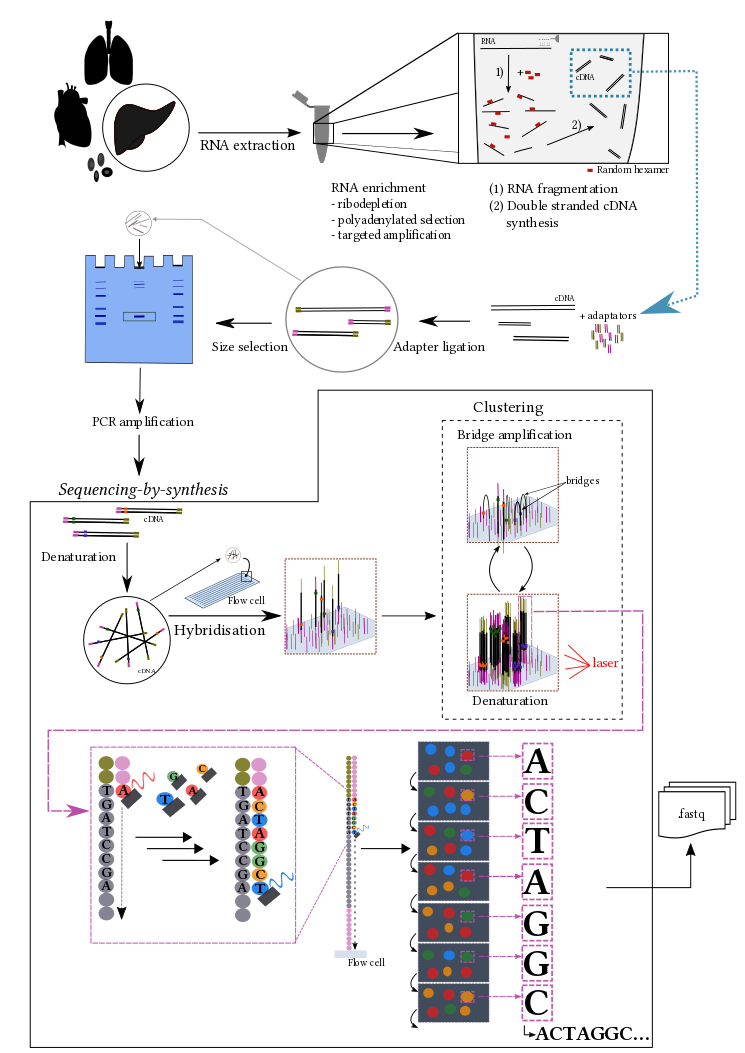
\includegraphics[scale=0.60]{introduction/IntroWorkflow.png}\centering
    \caption[Overview of a \Rnaseq\ workflow: library preparation
    and sequencing]{\label{fig:OverviewRnaseqPrepSeq}\textbf{Overview of
    a typical \Rnaseq\ workflow:
    library preparation and sequencing}}
\end{figure}

\NB Albeit the collection and the conservation of the samples prior to the
\gls{RNA} extraction most definitely affects the final estimations,
I will let aside these steps from my review.

\subsubsection{Library preparation}

While there are sequencing technologies that can directly sequence \glspl{RNA}
(see \mycite{rnaDirectSeq}), most of the technologies handle only \gls{DNA}.
Hence, the first step of a typical \Rnaseq\ workflow is the preparation of
\gls{cDNA} libraries from the starting material. This step and the sequencing
itself are the most platform dependent parts of the overall protocol.
Indeed, contingently on to the sequencing principle they rely,
the sequencers need the libraries to be fixed and loaded differently.

\minisec{\gls{RNA} extraction}
There are many methods to extract \glspl{RNA} from the primary samples and they
are commonly standardised. Indeed, regarding the type of biological samples,
the \glspl{RNA} of interest, the aim of the  study and the sequencing platform
used, there is one (or more) available commercial kit. These are designed in
a way to not interfere
with any of the later steps of the library preparation or with the sequencing
itself.

Without surprise, the choice of one kit (and hereby method of extraction)
over another can impact the final \Rnaseq\ data. The main difference between
the most widespread methods being the quantity of non-mature \glspl{RNA}
(\ie\ with longer intronic regions) detected whereby kit has been used.
However, the relative gene expression levels are similar from one extraction
protocol to the other. \mycite{RNAextraction}


\minisec{\gls{RNA} enrichment}

After extracting the \gls{RNA} from the cells or tissues,
the next step is to enrich the content of the samples with the \glspl{RNA}
of interest (\ie\ the concentration of the \glspl{RNA} of interest is increased
either by specifically selecting it or by removing other \glspl{RNA}). Indeed,
the \glspl{rRNA} are the most abundant type of \gls{RNA} in any cell. Even
though they amount for a very small part of the genome\footnote{For example,
\species{Homo sapiens}, there are 568 genes (<1\%) that are described as
\gls{rRNA} out of the 63,898 annotated genes of the ENSEMBL database
(\hg{38.p10} - \ens{89}).}, they represent by their number 70\% or more of
the total population of \gls{RNA} \mycite{biochbook}.
Although there are interests to study \glspl{rRNA} (\eg\ \mycite{rrnaStudy}),
\mRNAs\ studies are more
popular and they only constitute about 3 to 5\% of the whole \gls{RNA} population
\mycite{molBiolCell}. Other studies research even scarcer kinds of
\gls{RNA}.\footnote{Out of the 10,081 experiments tagged as \comp{``rna assay''}
and \comp{``sequencing assay''} within \gls{ArrayExpress}, 7,981 were also
tagged as \comp{``RNA-seq of coding RNA''}, 1,829 as \comp{``RNA-seq of
non coding RNA''} and 366 have both tags. 4 of them are only described as
\comp{``microRNA profiling by high-throughput sequencing''} --- Query date: 22
June 2017.}

There are typically three strategies to achieve \gls{RNA} enrichment:
either by polyA-selection, by ribodepletion or (more complex)
by targeted amplification. While these
approaches are insufficiently specific to select one particular kind of \gls{RNA}
or remove all \glspl{rRNA}, it eases and improves the downstream analyses.

\subminisec{PolyA-selection}
This strategy essentially targets the \mRNAs. It exploits the polyadenylated
tail at the 3' end of the \mRNAs\footnote{And a few other kinds of \gls{RNA},
\eg\ \glspl{lncRNA} \mycite{polyAlncRNA}} that is added
post-transcriptionally. In fact, magnetic beads supporting short
strings of thymine (oligo-dT) capture efficiently these \mRNAs\ while the others
are washed away \mycite{Mortazavi2008}.

This protocol is probably the most widespread one as it is the easiest and
cheapest to set up. A dataset produced following this protocol is known as
a \emph{polyA-selected} dataset.

\subminisec{Ribodepletion}
This strategy is preferred for the study of any \gls{ncRNA} or when researching
the interaction of \mRNAs\ with other \glspl{RNA} \mycite{ribodepletion}. This
strategy is in a way the reverse of the previous one as its also
uses magnetic beads, but this time to efficiently\footnote{ThermoFisher claims
that its RiboMinus protocol can remove till 99.99\% of the \glspl{rRNA}.}
target the unwanted \glspl{rRNA} as to remove from the sample.

The ribodepletion can also be achieved through ribonucleases. These enzymes
specifically digest \glspl{rRNA} and then \glspl{RNA} of interest can be retrieve
through size selection.

Datasets produced following a ribodepletion protocol are usually called
\emph{whole \gls{RNA}} or \emph{total \gls{RNA}} as a contrast to the
\emph{polyA-selected} ones.

\cite{castleData} created a total \gls{RNA} dataset but they use another
approach where they amplify \emph{every} other \gls{RNA} with the help of
specifically designed probes (see \cref{subsec:castlepresentation}). Hence,
the protocol they have used is closer to the following one.

\subminisec{Targeted amplification}
Targeted amplifications rely on primers that would be designed to target (or
avoid as for \cite{castleData}) specific sequence motifs of the genome. Most
studies based on this kind of approach are not referred as \Rnaseq\ studies, but
a name that is based on the studied \gls{RNA} type (\eg\ \gls{miRNA-Seq}) or
that emphasises the variation of the method (\eg\ Capture-Seq
\mycite{captureSeq}). Often, in comparison with a polyA-selected or ribodepleted
dataset, additional steps are required to prepare the libraries.


\minisec{RNA fragmentation}
Most of the sequencing platforms\footnote{As for the Illumina platforms that have
produced the transcriptomic datasets studied in this thesis.} require relatively
short (\ie\ 200 to 500 nt) length to sequence. Concomitantly, it also ensures
that the sampling along the \gls{RNA} is more uniform.
This fragmentation can be carry out via divalent cations hydrolysis or
nebullisation.

This step is performed on occasions after the \gls{cDNA} synthesis
(see next section). In those case, the \gls{cDNA} are fragmented mostly
by digestion with DNase I or by sonication.

\minisec{Double-stranded cDNA synthesis}
The \gls{RNA} molecules are used as a template for a retro-transcription
involving oligo-dTs or \emph{random} hexamer primers, respectively only
for polyA-selected datasets or any dataset (polyA-selected included).
The set of \emph{random} hexamer has been designed to cover the whole
transcriptome. Unfortunately, these \emph{random} hexamer primers have been
proven to actually lack full randomness \mycite{notSoRandom}.

At the end of the most common protocol, the order of synthesis of each \gls{cDNA}
strands is lost, \ie\ it is impossible to distinguish which of the \gls{cDNA}
strands has the same sequence than the original \gls{RNA}. Several techniques,
called \emph{strand-specific}, have been developed to compensate for this
(\mycite{strandSpecific}, \mycite{strandSpe}).

\minisec{Adapter ligation, PCR amplification and size selection}
After generating blunt edges by restriction digest of the \glspl{cDNA}, adapters
(small known sequences of oligonucleotides) are ligated to their both ends.
These adapters are constituted from several parts. A subset of them are ensuring
later the hybridisation of the \glspl{cDNA} with the flow
cells\footnote{\gls{flow}: see \cref{subsub:HybridClustAmp}.} (based on sequence
complimentary) and another set of them
are sequence binding sites that are used as primers for the following cluster
amplification step occurring \latin{in situ}. These adapters are also used to
introduce additional motifs such as indexes.

The next two steps can be interchanged regarding the amount of starting material
at disposition. All the molecules are amplified by \gls{PCR} before (or after)
a size-selection is performed (per gel electrophoresis) to extract
length-complying fragments (about 200 to 500 bp) to the sequencer machine
requirements\footnote{Indeed, the previous fragmentation step creates a great
length range of fragments.}.

Unfortunately, the size-selection means that any
transcript with an original length below the threshold used for the
selection will be missed\footnote{There is no problem for the greater length
as statistically they will present fragments that will be in the correct range.}.
For example, \glspl{miRNA} are shorter than the general requirement of Illumina
sequencers. Alternative protocols are addressing this issue
\mycite{smallRNAprotocol}.

\minisec{An example of alternative preparation strategy}
Along with the targeted, the strand-specific and small \glspl{RNA} protocols,
there are a few other variations to this typical protocol to handle other concerns.
For example, it is occasionally necessary to sequence simultaneously (in a single
run) multiple samples. This can be motivated by practical reasons
(to lower the experimental costs or hasten the overall processing time)
\mycite{multiplexCheaper} or critical to the experimental design as a way to
experimentally handle the \emph{batch effects}\footnote{Batch effect: see
\cref{subsub:BatchEffect}} \mycite{multiplexBatchEffect}. However, it is
crucial to later extricate the several pooled samples from each other as a
requirement to many downstream analyses.

\emph{Multiplexed} protocols easily achieve
the distinction between the multiple samples as they incorporate \emph{barcodes}
before ligating the adapters. These barcodes are also small sequences of
nucleotides and each sample has its own unique associated
barcode. In practice, each sample is prepared separately with the added extra
step (before the adapters ligation) where the barcode is incorporated, then all
the samples are pooled together before the next step that consists to hybridise
the \glspl{cDNA} to the flow cell.

Other extra steps occur just after the sequencing and before any other data
analysis: all the reads\footnote{Reads : see \cref{subsub:sequencing}} are
separated in files based on their barcodes and the barcode, along with the
adapters, is trimmed from all the reads.

The main inconvenient of the multiplexing protocol is that the original sequenced
length of the \glspl{cDNA} are then shorter as the barcodes are also (and have
to) be sequenced as well.

\subsubsection[Clustering: Hybridisation and Bridge amplification]{Clustering:
Hybridisation and Bridge amplification \mycite{IlluminaYoutube}}
\label{subsub:HybridClustAmp}

Once the libraries are ready, they are loaded onto a \emph{flow cell}\footnote{%
\emph{Flow cells} are the support of Illumina sequencing. They enable the
parallelisation of the sequencing of millions of \gls{DNA} fragments together
which are kept spatially separated in clusters. This was allowed with the advent
and optimisation of supported Chemistry. Each flow cell is a glass slide with
lanes. Each lane is coated with two short nucleotide sequences. One of these
oligonucleotides is complementary to a region comprised in the ligated adapters.}.

The clustering step comprises two phases: hybridisation and bridge amplification
of the \gls{cDNA} fragments.

\minisec{Hybridisation}

The double-strand \glspl{cDNA} are denatured and then each fragment randomly
hybridises across the flow cell surface with one of its small oligonucleotides.
These are used as primers for polymerases which create a first complimentary
strand to the hybridised \gls{DNA} fragments. The new double-strand molecule is
denatured and the original first template is washed away.

\minisec{Bridge amplification}
The strands then folds over and their (second) adapter hybridises with a
complimentary oligonucleotide sequence of the flow cell and thus creating a
bridge. The flow cell complimentary fragment is then used as the primer for a new
strand. The new double-stranded \gls{DNA} is then denatured (which
dismantles the bridge). Each of the two tethered molecules creates a new
bridge by hybridisation which are the templates for a new strand each.
This process happens many times and simultaneously for millions of fragments.
It creates clusters of clonal amplification of the original fragments of
the library. After the bridge amplification, the reverse strands are cleaved
and washed away. The 3' end primers are also blocked to avoid any unwanted
priming.

\subsubsection{Sequencing-by-synthesis}
\label{subsub:sequencing}

Illumina sequencers propose two sequencing approaches: single-end and paired-end.
The difference is that in \emph{single-end sequencing}\footnote{Chronologically
the oldest method}, the sequencing begins at one (and only one) of the fragment
ends and progresses towards the second. Whereas in \emph{paired-end sequencing},
once the first end has been sequenced (as in the single-end approach), after a
single new bridge replication, the other end of the original fragment is
sequenced as well. Hence, in paired-end, the sequencing occurs at \emph{both}
ends of each original fragment. This has been allowed by a small change in
the original single-end adpters \mycite{pairedEndAdapters}.

Though more expensive and more challenging to programmatically handle,
the paired-end approach produces more information and hence facilitates
the detection of genomic rearrangements (as indels or inversions) and
repetitive sequence elements.
It also allows an easier distinction between isoforms of a same gene and provides
greater support to the novel transcripts (new isoform or new gene) and fusion
genes\footnote{A \gls{fusionG} is a gene that is the product of the fusion of
parts of two different genes.}.

In both cases, the sequencing process is the same. It is an Illumina proprietary
process and it is called \emph{Sequencing-by-Synthesis} \mycite{seqBySynth}.
It uses the \gls{DNA} replication mechanism with modified \dNTPs.
It relies on the step-by-step incorporation of
reversible fluorescent tagged \dNTPs\ who are protected at
their 3'end to block any further elongation.
The product of this synthesis is called a \emph{read} and it supports the base
calling.

The sequencing occurs simultaneously on every identical fragment
of every cluster of the flow cell.
It begins with the hybridisation of a complimentary 5' primer onto the 3' biding
site of the tethered \gls{DNA} template. This primer is then extended by
replication to create a new read. Next, the sequencing cycle (described below)
repeats itself several times.

The \emph{sequencing cycle} starts with the addition of one complimentary
fluorescent \dNTP\ to the new growing read and, since the \dNTPs\ are blocked at
their 3' end, the replication process stops. Afterwards, all the unlinked
\dNTPs\ are washed away. Then, the clusters are excited by a light source
and as each
\dNTPs\ has a fluorescent tag with its own characteristic wave-length, the
signal that they emit back will allow to \emph{call} (\ie\ identify) what is the
new nucleotide that each cluster has incorporated. The signal intensity, along to
its wave-length are recorded (both of them are needed for the base calling
process for the base call itself and its associated accuracy). Finally,
the fluorescent tags and the 3' caps are cleaved
and washed away so a new cycle can happen.
The number of cycles determines the final length of the reads.

Unfortunately, as the sequencing proceeds, the error rate of the sequencers
increases. This is due to the incomplete removal of the fluorescent signal which
increases the background noise and thus reduces the signal-to-noise ratio.

Once the programmed read length is achieved (typically between 25 to 200 nt),
the reads are washed away (after denaturation).

\NB The below steps are specific to the \emph{paired-end} protocol.

Then, after introduction of a new primer, the first index is sequenced
following the same sequencing cycle.
Once completed, the index read is washed off and the 3' end primer is deprotected.
Then, the \gls{DNA} fragment bends over and hybridises to a complimentary
oligonucleotide at the surface of the flow cell.
Next, the second index is sequenced and its product read washed away,
a single new bridge replication follows.
The new double-stranded \gls{DNA} fragment is denatured and the 3' primers are
protected before the forward strand is cleaved and washed away.
Finally, the reverse strand is sequenced following the previously described
sequencing cycle. Once the same number of sequencing cycles than the forward
strand is reached, the read product of the reverse strand is washed away.

\subsubsection{From analogous input to digital output}

At the end of the sequencing process, the set of images (one per sequencing cycle)
is produced. While it is possible to work with the images themselves, in most
cases, the sequencing facilities will perform the base calling and provide the
end-user with text files. In single-end sequencing, there is one file per sample.
In paired-end sequencing, the reads are separated based on their associated
indexes into two ordered files: all the reads from the forward strands (one end)
are grouped in one file, and the ones from the reverse strands (other end)
in another.

These files are usually distributed in \fastq\ format
\mycite{fastqFormat} which record for each cluster (read) a unique identifier,
a nucleotide sequence and a \gls{Phred} quality score for each base of the
sequence. A few optional information can also be provided (\eg\
the position of the read on the \gls{flow} (See \cref{sec:fastq_format} for
a random read example).

The \gls{Phred} quality score ($Q$) measures the accuracy of the identification
of the nucleobase to which it refers. These score are set by the base calling
program and are defined as $Q = -10\log_{10}(P)$ with $P$ the probability of
the base being called wrongly. There are several possible encoding formats
(See \cref{sec:PhredScore}).

\subsubsection{Data analysis}

From the reconstruction of the
transcriptome to the normalisation of expression in each sample, the various
steps may be addressed through a number of different algorithmic approaches.
Often, the choice of a method at one stage implies a more limited number of
alternatives from which to pick at later points in the pipeline. Actually,
the choice is frequently driven by the kind of downstream analyses planned for
the study. More than the practical format of the data for these, it is the
assumptions and the correction methods used upstream that are critical for a
rigorous investigation and, later, for an accurate interpretation of the results.
%Hence, \Rnaseq\ data analysis pipeline are often designed in the chronological
%order of its steps than reversely.

\Cref{fig:pipelineTrans} present an example of the overall \latin{in silico}
process of raw \Rnaseq\ data. It summarises the steps and highlights the tools
I used to process the data within this thesis.

Before any downstream analysis, for each read, the genomic region (or
\emph{locus}) from which it has been originally expressed need to be identified.
Indeed, \Rnaseq\ main objective is to quantify the expression of genomic
\emph{features}\footnote{These genomic features could be genes, isoforms,
exons, novel genes, \dots\
In short, any genomic region with an annotated function.}. In other words,
the transcriptome needs to be reconstruct from the short reads and annotated
(\ie\ identify which features have been expressed in each library).

Two main different strategies (see further `Reconstruction strategies' segment)
manage to accomplish this identification step. Independently of the
approach, this step is the most challenging and time consuming
of the workflow. Tools, that tackle the reconstruction, usually provide a
number of tunable heuristic parameters (\eg\ maximum number of allowed mismatches
or indels per read before discarding a possible identification\footnote{Indeed,
many reads will have many identifications, these reads are defined as
\emph{ambiguous reads}.})
to speed up the task.
Unfortunately, as on Illumina platforms, the base calling accuracy decreases
along the read length, this may lead to an information loss \mycite{TrimRNAseq}.
To prevent informative reads to be discarded, it is opportune to perform a quality
check of the raw data prior to the identification step. Thus, reads with a drop of
accuracy in their 3'end may be shortened (\ie\ trimmed) and rescued for the next
reconstruction step. Similarly, low quality reads may be discarded hence
lowering the complexity
of the reconstruction task and hasten its accomplishment.

\minisec{Quality check, trimming and filtering}\label{minisec:trim}

The quality assessment allows to remove any read (or part of it) that would
increase the complexity of the reconstruction step or skew the downstream analyses.

It is wise to discard uninformative reads, \ie\
reads with a low sequence complexity (\eg\ poly-T or poly-A tails) or with
uncalled base (N). Indeed, these reads will hamper the processing time as they
usually map to several parts of the genome while also decreasing the accuracy of
the global gene expression estimations.

For similar reasons, it is judicious to remove reads with a low overall quality
score\footnote{It may vary based on the complete set of reads to analyse.}.

It is also prudent to check and remove any read that may map to possible
contamination sources\footnote{For example, for eukaryotes, by aligning (see next
segment) every read to the \species{Escherichia coli} genome}).
Indeed, as these reads are ambiguous, it is safer
to discard them than skew the expression estimations.

Finally, as a number of tools (mappers in particular) only accept reads
with an unique length, the purity-length balance requires optimisation.
Indeed, the trimming has to compromise between
an approach too lenient (where many unfit reads are discarded
by the mappers at a later step) and
a too stringent one (where too little reads are left for a pertinent analyses or
where shorter reads increase the overall complexity and therefore hinder
the mapping both on time and accuracy \mycite{Trimwisely}).

\NB Generally, after the sequencer calls the reads, a first trimming removes
all the adaptors and barcodes needed by the sequencing protocols. Thus,
in principle, they are not to be found in the ``raw data''.
However, to avert any latter contingency, a research against
a list of the most common adaptors and an over-representation assessment of small
sequences (\emph{k-mers}\footnote{\emph{k-mer}: In the present context, all
possible subsequences of length
\emph{k} of a \emph{read}.}) at each end of the reads is good practice.


\minisec{Reconstruction strategies}

Two main approaches can be used for the very computationally expensive step of
identification. I will present them in a decreasing order of complexity:
the \latin{de novo} assembly of the reads and then the Reads alignment approach
(to a genome reference or a transcriptome one).

Regardless of the approaches, the reconstructed transcriptome is usually reported
as a \emph{SAM} file \mycite{SAMformat} (or one of its derivative format either
\emph{BAM} or more recently \emph{CRAM}).

\begin{figure}
    \includegraphics[scale=0.60]{introduction/MappingStrategies_cropped.pdf}\centering
    \caption[Overview of main reconstruction strategies for
    \Rnaseq\ transcriptome]{\label{fig:OverviewRnaseqMapping}\textbf{Overview of main
    reconstruction strategies for a \Rnaseq\ transcriptome}}
\end{figure}


\subminisec{\latin{de novo} Assembly}
This approach is favoured when the reference genome of the species of interest
is unavailable or of poor quality
(\eg\ many non-model organisms) or inadequate (\eg\ cancer samples)
for the samples of interest. However, if a reference already exists this strategy
is avoided to the utmost.

It allows the unbiased discovery of novel
exon-exon junctions \mycite{deBruijn}. As none of the datasets I use in this
thesis has been reconstructed through this approach, I briefly summarise
the main points below as more in-depth reviews cover this strategy
\mycite{denovoReview}.

In \latin{de novo} assembly, the reconstruction of the transcriptome happens
with the construction of the longest possible \emph{contigs} (\ie\ contiguously
expressed regions) based on sets of overlapping reads. Short length reads add
to the overall complexity of this approach. While paired-end reads may help to
solve a number of genomic regions, lowly expressed or repetitive regions remain
challenging to determine. There are several algorithmic approaches for \latin{de
novo} transcriptome assembly \mycite{algorithmsDenovo},
though the most prevalent one is the de Bruijn representation \mycite{deBruijn}.


\subminisec{Read alignment}
This approach exploits prior knowledge. The reads are aligned to a reference to
hasten the reconstruction process. The reference may be a genome or a
transcriptome (provided that a good annotation is available).

\subsubminisec{Genome reference}
Aligning to the genome allows to discover new genes or isoforms. However, it
requires a splice-aware algorithms, \ie\ they need to align the
reads across the splice-junctions (which is possible but non-trivial).
As illustrated in \Cref{fig:OverviewRnaseqMapping} --- Genome alignment part,
the reads might span a number of discontinued regions of the reference.
While on one hand, aligning to the genome avoids \emph{multiple mapping
issues}\footnote{Due to sequence similarity, a same read or subpart of a read
may be attributed to a number of different loci in the genome. As it is
impossible to directly attribute the read to its original locus of expression,
distribution models have to be pondered to avoid unnecessary skewness while
the quantification step.} for a same exon. Indeed, irrespectively of the number
of a gene isoforms including an exon, the sequence of this exon is transcribed
only once in the reference. However, this also implies that, for correct
quantifications of the different isoforms, the genome needs to provide the
coordinates for the isoforms and that an accurate quantification at isoform levels
requires further analysis.


\subsubminisec{Transcriptome reference}
Using a transcriptome as reference instead of a genome reduces the complexity
of the aligning step due to the lack of intronic sequences. However, it also
limits the potential downstream analyses, \eg\ any new (or unannotated) gene
or isoform will be missed. This approach is the easiest, but a pre-existing
accurate and well-annotated gene models is required. The third part of the
\Cref{fig:OverviewRnaseqMapping} shows in fact that this approach is simpler
to the previous one as a direct alignment of the reads is done against the
transcriptome of reference. This enables to quantify accurately the expression
of gene isoforms, provided that the gene model is correct and the reads may be
attributed unambiguously to a single isoform for each gene.


To mitigate between very computational greedy approaches and more constraining
ones, several tools complementary use the previous strategies.

\subminisec{Hybrid approach between \latin{de novo} and alignment}
There are tools like \soft{TopHat2}\footnote{\soft{TopHat} ---
\href{https://ccb.jhu.edu/software/tophat/index.shtml}%
{https://ccb.jhu.edu/software/tophat/index.shtml}} (2.0.12) \mycite{tophat2}
(which has been used to reconstruct all the
transcriptomes involved in this thesis --- see \Cref{ch:datasets}),
that uses an hybrid approach between a reference alignment and a \latin{de novo}
assembly. As a first (but optional) step, \soft{TopHat2} tries to contiguously
align the reads with \soft{Bowtie}\footnote{\soft{Bowtie} ---
\href{http://bowtie-bio.sourceforge.net/index.shtml}%
{http://bowtie-bio.sourceforge.net/index.shtml}} \mycite{Bowtie}
to the reference transcriptome when this one is provided. Then
(or alternatively as a first step), the unmapped reads are aligned to the
reference genome. The intention in these alignment steps is to identify and
localise the exons, which may eventually span over splicing junctions and be
connected through spliced alignment. Then, \soft{TopHat2} builds a database of
possible exon-exon splice junctions from the set of mapped reads and then split
the remaining unmapped (or aligned with a low score) reads in order to find
possible new split events via a seed-and-extend approach. Potential new events
are considered when smaller segments, that are matching exactly the reference
in their good quality score regions, are also overlapping a splice junction
reported in the newly created database.

The smaller segments
have to match exactly for their regions with good quality score with the reference
and have overlaps (for an user defined length) with a splice junction.
These segment sections are called seed.
Any read with a seed is then checked for a
complete alignment to the exons on both side of the junction.

In the case of paired-end data, each read is first processed separately. Although,
they are a valuable resource in a final evaluation phase, where with additional
information sources, they help to determinate among the many possibilities which
are the most credible ones.


\minisec{Quantification of \emph{features}}

With \Rnaseq\ data, the typical next step after mapping the reads to the
reference is to quantify the expression of the feature\footnote{E.g.\ genes,
isoforms, exons, spicing events, \ldots}
of interest. In fact, while genotyping, heredity
studies and other genetic focused studies are in principle possible, the usual
main focus is centred on expression\footnote{For example, instead of reporting
a specific \gls{SNP}, in an \Rnaseq\ study, the core interest is more usually
about the specific allelic expression.}. Moreover, most of the \Rnaseq\ studies
lack to provide the sequence depth and coverage for such studies.
Genome assays are by far better for those.

Several tools and algorithmic approaches are available. Within this thesis, I
use two popular tools, \soft{HTSeq-count}\footnote{\soft{HTSeq-count} ---
\href{http://www-huber.embl.de/HTSeq/doc/index.html\#}%
{http://www-huber.embl.de/HTSeq/doc/index.html\#}} (0.6.1p1)
\mycite{htseq} and
\soft{Cufflinks}\footnote{\soft{Cufflinks} ---
\href{http://cole-trapnell-lab.github.io/cufflinks/manual/}%
{http://cole-trapnell-lab.github.io/cufflinks/manual/}} (2.2.1)
\mycite{cufflinks},
which are both compatible with \soft{TopHat2} but rely on different concepts.

\TK{review about the quantification tools}

\subminisec{HTSeq-count}
This

\subminisec{Cufflinks}



\minisec{Normalisation}



\rew{Angela:
Alignment to the genome results in a set of one or more genomic coordinates for
each aligned read which may or may not span exon junctions. By itself this
information is of limited use so alignments can be further matched to known
annotated features (for example by searching for overlaps between aligned reads
and genes) or they can be used to build gene models de novo. One of the earliest
and most well known programs to achieve the latter is a software application
called Cufflinks [146]. In this program the authors have implemented an algorithm
which tries to find the smallest possible set of transcripts that explains all
observed (aligned) read or read pairs (henceforth in this section referred to
as fragments). As in the de novo assembly approach described above, the fragments
are used to find islands of expression. The problem of assembly is then to
construct a directed acyclic graph in which fragments are nodes and pairs of
nodes are connected if the fragments overlap with one another and if they do not
imply splice junctions which cannot be present simultaneously in the same
transcript (i.e. if the aligned reads are not incompatible, Figure 1.7). Assembly
with Cufflinks is done independently for each island.
Finally, Cufflinks finds the minimum number of partitions into chains of the
graph by implementing a proof of a theorem for the decomposition of partially
ordered sets known as Dilworth’s theorem. This set of minimum number of paths
however may not be unique as in the example in Figure 1.8. In order to “phase”
distant exons together Cufflinks chooses the path that minimises the total cost
obtained by weighting each graph edge between nodes x and y with a cost C(x, y)
= − log(1 − |φx − φy |), where φx and φy are the percent-spliced-in metrics
computed for x and y by dividing the number of alignments compatible with x or y
by the total number of fragments overlapping x or y and normalising for the
length of x or y.
The method employed by Cufflinks requires high coverage (high read overlap) to
create good gene models, otherwise lowly expressed transcripts will be broken
into pieces. Still, at low coverage this method is more sensitive than the de
novo assemblers of the previous sections [134]. One other caveat of this approach
is that paths are maximally extended as in the example of Figure 1.7, making it
impossible to detect some instances of alternative transcript start and end
sites. Finally, Cufflinks finds the minimum set of transcripts that explains the data.
Choosing the simplest model over a more complex one when both models are equally
valid is an application of Occam’s Razor. However, while Occam’s Razor is of great
use for the development of theoretical models, its adoption for arbitrating
between models in biology is controversial since the result of evolution is not
necessarily optimal [157].}



\subsection{Proteome exploration with Mass spectrometry}


\begin{comment}
\subsection{Proteomics}
    \subsubsection{Main technologies}
    \subsubsection{Mass sprectrometry}

\end{comment}

\section{Big studies, big data and Reproducibility}



\subsection{Reproducibility issues // experimental design}
    \subsubsection{Batch effect}\label{subsub:BatchEffect}
    Batch effect: \mycite{batchEffect}

    \begin{itemize}
            \item{Different samples}
            \item{Technology: wet lab but also software: Rupgrade, \ldots}
            \item{missing meta-data}
        \end{itemize}
    \subsection{Main concerns}
        \subsubsection{Detection}
        \subsubsection{Quantification}
    \subsection{Consistency through biological layers}

\mycite{reviewRNAseqBestpractice}
\subsection{Co-studies on Transcriptomics and Proteomics in the literature}
\subsection{EBI Expression Atlas or how integrating independent datasets }




\section{Reproducibility vs. Repeatability}


\section{Experimental design}
\subsection{Technical replicates}
\subsection{Biological replicates}
pourquoi c'est important




\section{discussion or conclusion}


\Rnaseq\ as \Dnaseq\ needs many corrections as to prevent biases in the downstream
analysis. However, due to the dynamic component of the transcriptome
contrarily to the genome, while it is possible to apply the corrections in
\Dnaseq\ and then analyse the data \mycite{dnaseqCorr},
in \Rnaseq, corrections are already part of
the analysis and requires often as much skills than flair. It is possible that
future protocols will overcome this issue.


\section{Aims of the thesis}

One main focus of my work for this thesis was to appraise the
consistency of findings that have been enlightened in normal Human tissues by
individual large scale transcriptomics and, more recently, large-scale
proteomics studies.

While the amount of data to process and integrate can be challenging,
paradoxically the data available to draw statistically significant conclusions
is often still too sparse. However, we do have enough to provide at least a
qualitative assessment of the consistency and evaluate the feasibility of a
quantitative assessment in general, if not, realise a quantitative integration
for a few key tissues.

\section{Achievements}
\begin{itemize}
    \item First time so many datasets have been reprocessed together with the
        same annotation and hence comparison are better (y'a le truc de chez Burges,
        mais ils se sont concentré sur une petite partie des genes)
    \item surtout comparison of Gtex and Uhlen (aussi approfondi)
    \item reprocessing of all the proteome untargeted in human
    \item comparison entre protein expression and 2 datasets (meilleur que le
        science report dans le sens où il y a pas de polémique
    \item siteweb//application de visualisaiton de la comparison
    \item liste croisé de tissues specifique et house keeping à travers datasets
        transcriptomic et protoemic
    \item attempt de normalisation basée sur les housekeepings
\end{itemize}

\chapter{Available high-throughput normal human datasets}\label{ch:datasets}

\begin{comment}
\setlength{\epigraphwidth}{0.8\textwidth}%0.57
\setlength{\epigraphrule}{0pt}%0.1
\epigraphhead[70]{%
\epigraph{Data! Data! Data! I can’t make bricks without clay!}{Sherlock Homes\\
(Sir Arthur Conan Doyle)}}
\end{comment}


In the past few years, many laboratories have studied the expression
of genes within normal humans at the transcriptome and at
the proteome levels by taking advantage of high-throughput techniques
(\eg\ \citet{Krupp2012,VTpaper,ramskoldan:2009,Uhlen2014,%
Uhlen2015,UhlenGastro,GTExTranscript,PeptideAtlas,PandeyData,KusterData}).
In this chapter, I review the openly available (for research) data
I use within my thesis
and explain how they have been reprocessed.
Besides the results I report in the subsequent chapters,
the present chapter also provides the basis for work
I have co-authored\footfullcite{Wright-2016}.

Unless otherwise stated, all the computational processing of the \Rnaseq\ part
described here have been performed by myself under the supervision of
\alvis. I also received general feedback from \mar,
\johan\ and \nuno. The proteome data has been processed by \james.


\section{Introduction}

Every dataset with which I have worked fits three main criteria.
Firstly, they comprise normal (\ie\ reported as disease-free) human samples
from at least three different tissue types.
Secondly, gene expression
quantifications are based on \Rnaseq\ for the transcriptome and on label-free \ms\
for the proteome\footnote{These
technologies are non-targeted high-throughput and
allow one, in theory, to study the whole
repertoire of \glspl{RNA} or proteins in a sample.}.
Finally, the \emph{raw} data is openly available and reusable\footnote{%
In this context, \emph{reusable} means that the data can be processed
as accurately by third-party researchers than the original authors,
and this without the need to access additional information
that have been not openly released}.


In the next section, I first describe the \Rnaseq\ and the \ms\ data I use
in my thesis; then I detail how these data have been processed to be
employed in the next chapters for various analyses that explore the transcriptome,
the proteome and finally, the comparison and integration of these two
biological layers.


\section{Transcriptome RNA-Seq studies}\label{sec:rnaseq-data}

During the data selection process,
I had to disregard a few studies as the raw data was not fitting
the reusability criterion \mycite{Burge,Pan2008-di}.
Many times I came across studies with ambiguous encoding
format for the raw data such
as the \ArrayExpress{E-GEOD-41637} dataset~\mycite{Burge}.
Despite my best efforts,
I was unable to resolve this issue
by contacting the respective authors.
\citet{Burge} (\ArrayExpress{E-GEOD-41637}) is one example of study
that I unfortunately had to dismiss.

I describe hereinafter the five transcriptomic datasets I used
in the chronological order of their first public release.
\Cref{tab:Trans5DF} summarises the main characteristics of these datasets.

\begin{sidewaystable}
           \centering
           \caption[General description of the 5 transcriptomic datasets
           (\Rnaseq) used for this study]{\label{tab:Trans5DF}\textbf{General
           description of the five transcriptomic datasets (\Rnaseq) used for this
           study}\\\footnotesize{Illumina Body Map (IBM) has no \enquote{regular}
           technical replicates as the \enquote{replicates} are the product of
           different protocols, thus are unfit to estimate the specific noise of
           either protocol (single-end or paired-end).
           \NB\ The protocols used for \Gtex\ and Castle datasets are not the same:
           \Gtex\ is following the most common ribodepletion protocol, while
           Castle is based on  a targeted amplification protocol.\\
           %\mynormalcheckmark\ indicates that the dataset presents the
           %characteristic, and \\(\mynormalcheckmark) that one (or more) of the
           %required criteria of the characteristic is lacking.\\
           }}
       \begin{tabular}{@{}cccccccccc@{}}
       \toprule
       \multicolumn{1}{c|}
           {\multirow{2}{*}{ArrayExpress ID}} &
            \multicolumn{1}{c|}{\multirow{2}{*}{Data ID}} &
            \multicolumn{2}{c|}{\begin{tabular}[c]{@{}c@{}}Library\\Preparation\end{tabular}} &
            \multicolumn{2}{c|}{Sequencing} &
            \multicolumn{2}{c|}{Replicates} &
            \multicolumn{1}{c|}{\multirow{2}{*}{\begin{tabular}[c]{@{}c@{}}Number of\\Tissue\\
                    Types\end{tabular}}} &
            \multirow{2}{*}{\begin{tabular}[c]{@{}c@{}}Multi-sampling\\ from the \\ same
            individual\end{tabular}} \\
            \cmidrule(lr){3-8}
            \multicolumn{1}{c|}{} & \multicolumn{1}{c|}{} &
            \multicolumn{1}{c|}{\begin{tabular}[c]{@{}c@{}}Total\\ RNA\end{tabular}} &
            \multicolumn{1}{c|}{\begin{tabular}[c]{@{}c@{}}PolyA\\ selected\end{tabular}} &
            \multicolumn{1}{c|}{\begin{tabular}[c]{@{}c@{}}Single\\ end\end{tabular}} &
            \multicolumn{1}{c|}{\begin{tabular}[c]{@{}c@{}}Paired\\ end\end{tabular}} &
            \multicolumn{1}{c|}{Biological} & \multicolumn{1}{c|}{Technical} &
            \multicolumn{1}{c|}{} &  \\
       \midrule
       E-MTAB-305 & Castle & \mycheckmark\ &  & \mycheckmark\ &  &  &  & 11 &  \\
       E-GEOD-30352 & Brawand &  & \mycheckmark\ & \mycheckmark\  &  &
           \mycheckmark\  &  & 8 &  \\
       E-MTAB-513 & IBM &  & \mycheckmark\ & \mycheckmark\ & \mycheckmark\ &  &
           (\mycheckmark) & 16 &  \\
       E-MTAB-2836 \footnotesize{(and E-MTAB-1733)}& Uhlén &  & \mycheckmark\ &
           & \mycheckmark\ & \mycheckmark\  & \mycheckmark\  & 32 &  \\
       E-MTAB-2919 & Gtex (v4)  &  & \mycheckmark\ &  & \mycheckmark\ &
           \mycheckmark\ &  & 54 & \mycheckmark\\
       \bottomrule
       \multicolumn{10}{p{.8\textwidth}}{\raggedright\
           \mynormalcheckmark\ indicates that the dataset presents the
           characteristic, and \\(\mynormalcheckmark) that one (or more) of the
           required criteria of the characteristic is lacking.}
      \end{tabular}
\end{sidewaystable}

\subsection{Castle et al.\ dataset}\label{subsec:castlepresentation}
\vspace*{-0.1in}
\citet{castleData} released this dataset along with their study:
\paper{\citetitle{castleData}}.
The authors were interested in exploring the whole RNA repertoire
with sequencing-based technology and they primarily focused their study
on the non-coding part.

Purchased \gls{RNA} extracts were used to create multiple-donors pooled
samples for 11 tissues from which total \gls{RNA} libraries were prepared
following a total transcriptomic protocol
where nonribosomal \gls{RNA} transcripts are
amplified specifically by \gls{PCR}~\mycite{Armour:2009}.

For each library (tissue), an average of 50 million sequence reads were sequenced
using an Illumina Genome Analyser-II sequencer (single-end).
The original reads were trimmed to 28 \gls{nt}
before being released through EMBL archives (\ENA{ERP000257}
and \ArrayExpress{E-MTAB-305}).

Despite several limitations, such as the lack of replicates, the old technology and
the short reads,
I have included this dataset for two main reasons.
Firstly, it is the oldest available
\Rnaseq\ data I found that was performed on normal human tissues.
Thus, the congruence of results for this dataset with the following ones
gives a rough idea on the extent of \Rnaseq\ datasets
that may be integrated together.
Secondly, as \Rnaseq\ studies are prepared mainly with polyA-selected protocols
nowadays, I was interested in gauging how the library preparation
protocols --- and the presence of \glspl{ncRNA} --- can affect the
quantifications and then any final observation.


\subsection{Brawand et al.\ dataset}\label{subsec:brawandpresentation}
\vspace*{-0.2in}
In the article entitled~\paper{\citetitle{VTpaper}},
\citet{VTpaper} focused their interest on the
evolution of the mammalian transcriptomes\footnote{While there were existing
studies on the matter, the sequencing approach was then creating new perspectives.}.

They collected 6 organs from 10 different vertebrates:
9 mammalians (including human) and a bird. There are no technical replicates,
but  two biological replicates per tissue:
one male and one female for every tissue except the testis (two males).
The 131 libraries (including 23 for \species{Homo sapiens}) were prepared with
a polyA-selected protocol.
Hence, they are largely enriched in \pcgs.

An average of 3.2 billion 76 \gls{bp}-long single-end reads were generated per sample
using an Illumina Genome Analyser IIx (single-end) and they released them
through \gls{GEO} (accession number: GSE30352).
I personally retrieved the human data from
\ArrayExpress{E-GEOD-30352}\footnote{ArrayExpress routinely was importing
datasets from \gls{GEO} on a weekly basis until very recently.
While not automatically, \gls{GEO} data are still included in \egxa.}.


\subsection{Illumina Body Map 2.0 (IBM)}\label{subsec:ibmpresentation}
\vspace*{-0.2in}
This dataset, created in 2010, has been released in
2011\footnote{See~\citetitle{ibmEnsembl} -~\cite{ibmEnsembl}} by Illumina
mostly to advertise its most recent technology improvement at that time:
the paired-end sequencing. Actually, until then, all the sequencing was done
from only one end of the \gls{DNA} or \gls{cDNA} fragments. From that
date, most of the following transcriptome studies based on \Rnaseq\ use
paired-end sequencing.

The dataset covers 16 tissues (one donor per tissue) and
the libraries were prepared following a polyA-selected
and are enriched in protein coding genes.

Although each sample has been sequenced twice and despite having in principle
\emph{technical} replicates, these are not ``regular'' technical replicates.
\emph{Technical} replicates, by contrast to \emph{biological} replicates,
usually imply that their processing uses the same sample source and protocols.
Thus, the error and noise due to a specific technique could be determined.
Here, however, each tissue has been sequenced once with a single-end protocol
and once with a paired-end one to compare their ability to discriminate between
\gls{mRNA} isoforms.
Indeed, Illumina's main incentive to develop its paired-end
technology was to improve the accurate identification of spliced \glspl{mRNA}.

The sequencing was performed with an Illumina HiSeq 2000, and the reads were
released through \ArrayExpress{E-MTAB-503} (\ENA{ERP000546}),
from where I have retrieved both the single-end and paired-end mono-tissue samples
(the original dataset includes raw data files for mixtures
that have been created with the tissue samples).

Despite the lack of biological replicates,
it was for an extended time
the most extensive freely available \Rnaseq\ dataset of human tissues.
Hence, it has been referenced many times
(\eg\ \citet{Asmann2012-in,ibmrelatedpaper,Smith2012-jw,Derrien2012-ej,%
Florea2013-in,tophat2,Kechavarzi2014-oi,Zhao2014-xj,Pasquali2014-zj,Corpas2014-ej,%
Petryszak2014-kj,Brown2015-co,Janes2015-wn,%
De_Simone2016-fb,Kern2016-dv,Iwakiri2016-sr,Yao2017-gj,Akers2018-cf})
in the literature since its release.
In fact, this dataset is the most viewed one in \gls{ArrayExpress}
(with 68,020 views on 31 May 2018 ---
the second most viewed dataset (46,247 views)
being \ArrayExpress{E-MTAB-62}\mycite{Lukk2010-op}).

\subsection{Uhlén et al.\ dataset}\label{subsec:uhlenPresentation}
\vspace*{-0.1in}
Uhlén et al.\ have created the
\hFo{Human Protein Atlas}{https://www.proteinatlas.org/}
(often referred as \glsxtrshort{HPA} in the literature).
This atlas revolves mostly around the spatial
distribution of the proteins through the human body.
Using diverse approaches and techniques, including \Rnaseq,
they first released \Rnaseq\ data for 27 normal tissues
as part of their study:~\paper{\citetitle{Uhlen2014}}%
~\mycite{Uhlen2014}.
Later, they extended the dataset with new samples and 5 new
tissues. The latest version was published within~\paper{\citetitle{Uhlen2015}}%
~\mycite{Uhlen2015} in \textit{Science}.

For each of the 32 tissues, there are (at least two) biological replicates.
With a few exceptions, the tissues have both male and female donors.
Many of the tissues present also technical replicates.
The total set comprises 200 samples,
which have been picked by pathologists
based on the screening of frozen biopsy samples.

The polyA-selected libraries were paired-end sequenced
with an Illumina HiSeq 2000 or 2500.
I first started to work with the early version of this dataset
(\ArrayExpress{E-MTAB-1733} --- 171 samples for 27 tissues),
and then I upgraded my work with the extended more recent version
(\ArrayExpress{E-MTAB-2836}).

At the preparation time of this thesis, this normal human dataset is the
most comprehensive, freely and publicly available dataset:
either regarding the number of tissues (see \Cref{tab:Trans5DF})
or the number of samples (see \Cref{tab:Lib5DF}).
Therefore, its growing number of references is unsurprising.

\subsection{GTEx dataset}\label{subsec:gtexPresentation}
\vspace*{-0.1in}
The Genotype-Tissue Expression (\gls{GTEx}) project is funded by the \gls{NIH}
Common Fund and aims to establish, in its authors' own words,
\textquote{a resource database and associated tissue bank for the study of the
relationship between genetic variation and gene expression
and other molecular phenotypes in multiple reference tissues}.
The project was first introduced in~\citet{GTEx2013}. It aims to quickly collect
various tissues from postmortem donors for genotype-tissue expression analyses
(notably \gls{eQTL} studies, which study the function of \glspl{SNP}
in the modulation of \gls{RNA} expression).
The results of the
analyses are released through the \hFo{\Gtex\ portal}{https://gtexportal.org}.

As the project is quite ambitious and the collection
and sequencing of the samples spreads over a long period of time,
several intermediate data \enquote{\emph{freezes}} have been
released\footnote{Many groups are involved in collecting, producing or processing
the data. To ease the communication and work coordination,
many time points are used to reference each a specific state (version)
of the data. Each version of the data is called a \emph{freeze}.}.
My analyses include samples up to the fourth release of the pilot phase (v4).
This release covers 54 tissues/cell types (53 normal and 1 tumoral)
collected on from individuals for a total of 3,276 samples.

The \Rnaseq\ libraries were prepared following a polyA-selected protocols
and have been paired-end sequenced on an Illumina HiSeq 2000/2500.
There is an average of 80 million reads per sample.

For privacy reasons, the raw data is available only through controlled access via
\dbGaP{phs000424.v4.p1} (access number specific to the version of the data I used
in my study).
Unfortunately, this translates to a slow access time to the raw data.

\section[Proteome Mass Spectrometry bottom-down studies]%
{Proteome Mass Spectrometry bottom-down studies \quad}\label{sec:ProteoData}

As mentioned earlier,
the proteomic data have been selected and handled by \jyoti\ and \james.

Until recently, compared to the transcriptome, the proteome world
was lacking in normal human tissues expression quantification
experiments. In fact, while there were human protein maps available
(\eg\ the \hFo{Human Protein Atlas}{https://www.proteinatlas.org}), these
are mostly reporting the spatial expression of proteins (as they are based
on immunohistochemistry or other means of identification) than quantifying
their (non-targeted) abundance in each tissue.

In 2014, two independent groups of authors~\mycite{PandeyData,KusterData}
published (in \textit{Nature},
issue 7502) their own \textquote{\emph{draft of the human proteome}}
based on the study of tissues with \ms. These two datasets complement a previous
smaller one that was publicly released but was never the object of a publication.

Hereinafter, I present these three datasets that I use in my thesis.
See \Crefp{fig:pipelineProt}{A} for a short summary.

\subsection{Pandey Lab dataset}

The Pandey Lab~\mycite{PandeyData} created the
\hFo{Human Proteome Map}{http://www.humanproteomemap.org} which
they released alongside~\paper{\citetitle{PandeyData}} in \emph{Nature}.

For their study, they processed 30 kinds of histological normal human
tissues and cell line samples (17 adult tissues, 7 foetal tissues and 6
haematopoietic cell types).
Each sample was created from pooling samples of three
individuals (generally two males and one female).

Their proteomic libraries were prepared with a label-free method to quantify
as many proteins as possible.
The samples were fractionated to protein level through \gls{SDS-PAGE},
and then at peptide level after trypsin digestion by \gls{RPLC}
to create 85 experimental samples.
Finally, state-of-art \gls{MS/MS} protocols
(with high-resolution and high accuracy
\glspl{FTMS} Thermo Scientific \orbi\ instruments)
was used to generate about 25 million of (\gls{HCD})
high-resolution mass spectra which account for 2,212 \gls{LC-MS/MS} profiles.
The raw spectra were retrieved from ProteomeXchange via the repository
\Pride{PXD000561}.

While the authors' effort to generate technical high quality raw data was highly
appraised by the scientific community, their processing
(identification and quantification) methods were heavily
criticised (see~\citet{Ezkurdia2014-qx,Deutsch2015}).
Thus, for this thesis I have relied only on
quantifications provided by \james\ who reprocessed the raw spectra.

\subsection{Kuster dataset}

In their approach of the human proteome map, the Kuster Lab~\mycite{KusterData}
combined newly generated \gls{LC-MS/MS} spectrum data (about 40\% of their
complete working set) with already publicly available data
(either from their colleagues or accessible through repositories
--- for the remaining 60\%).
They reprocessed
the whole collection of spectra to maximise proteome coverage
and make it available through their own repository:
\hFo{ProteomicsDB}{https://www.proteomicsdb.org/}.

The subset of data considered in my thesis is also
known as the [protein] Human BodyMap which is the part that the Kuster lab
primary generated for their own study. They collected 48 experiments covering 36
tissues (adult and foetal) and cell lines. After \gls{LDS-PAGE} fractionation and
digestion into peptides with trypsin, they processed the samples with
\gls{LC-MS/MS} to create 1,087 profiles.  Overall, that represents about
14 million of \gls{HCD}/\gls{CID} spectra from Thermo Scientific instruments
(including an \orbi).
This specific raw data subpart was downloaded from \Proteomicsdb{PRDB000042}.

\subsection{Cutler dataset}\label{subsec:cutler}

This dataset was generated prior to the \pandey\ and the \kuster\
data as it was released in 2011 through
\hFo{PeptideAtlas}{http://www.peptideatlas.org/}~\mycite{PeptideAtlas},
IDs: [PAe001768 --- PAe001778].

It was created by Paul Cutler at Roche Pharmaceuticals.
It comprises 10 different tissues (and one sample per tissue) that after trypsin
digestion, were analysed through Thermo Scientific \gls{LTQ}-\orbi.
In total, there are 1,618 \gls{CID} profiles which accounts for 13 million raw
\gls{CID} spectra from a \gls{LTQ}-\orbi\ instrument.

While this dataset was never published on its own, it has been used in different
studies (\eg~\cite{KusterData}).
The raw files were accessed and downloaded from \Proteomicsdb{PRDB000012}.


\section{Consistent processing pipelines}

The authors of these five transcriptomic and three proteomic studies have,
in most cases,
released the quantification of the expression values either directly
(\eg~\cite{Krupp2012}) or upon requests (\eg~\cite{PandeyData}).
Third-parties also distribute
quantification for these studies either retrieved from the original studies,
such as \hFoCi{BioGPS}{http://biogps.org/}{BioGPS1} or
\hFoCi{Harmonizome}{https://amp.pharm.mssm.edu/Harmonizome}{Harmonizome},
or after reprocessing the raw data as the \egxa~\mycite{EBIgxa} does.

To primarily reduce for avoidable technical variability,
and despite readily available quantifications for most of the
datasets, I only used data reprocessed from raw files by myself or \nuno\
(\gtex\ dataset) for the transcriptomic data and by \james\
for the proteomic data as already mentioned.

In fact, each study has been originally processed with different protocols,
\eg\ \gtex{}~\mycite{GTExTranscript} and \castle{}~\mycite{Krupp2012}.
While the \egxa\ reprocesses raw data through the same
methods and has nowadays quantification for most of the aforementioned
datasets (it is still lacking the \castle\ \etal\ one.),
these were still the products of different protocols when I started my work.
Indeed, the datasets were processed with different versions of
reference (Human genome build and annotation) and tools.

Intuitively, we expect that different processing protocols produce
different results.
As I started to work with \Rnaseq\ data,
I noticed many potential analysis variables that impact
at various levels the resulting gene expression values.
Indeed, many of these have been
reported in the literature since then; in fact,
annotation versions~\mycite{annotationDiff},
contamination (from viruses or bacteria \gls{DNA})~\mycite{contaminationRNAseq},
quality controls (and subsequent reads filtering choices)~\mycite{qualityRNAseq},
mapping and quantifications pipelines~\mycite{Fonseca2014}
have considerable effects on the final quantification. Lastly, normalisation
methods also greatly impact the final expression figures~\mycite{Dillies2013,%
normSigCancerHelp}. For all these reasons,
I decided to  reprocess all transcriptomic datasets with the same exact protocol
as the first step of my study.
Recently, \citet{Danielsson2015-cn} compare results based on prepublished data and
reprocessed ones and conclude that using a single processing pipeline ensures better results.

Likewise, there are various tools and many parameters for each processing step
needed to quantify the proteomic data
that may impact the final expression values~\mycite{Aebersold2011-av}.
For example, various search engines allow detecting
different sets of peptides~\mycite{Griss2016}.
\citet{Mackay2015-zl} has reviewed and analysed the impact
of many of these variables more specifically for label-free proteomics,
such as the effect of \gls{FDR}, protein inference tools or normalisation methods.
Therefore, the three datasets were reprocessed uniformly
from the raw spectra up to the normalisation of the protein expression values.

\subsection{RNA-Seq raw data processing}

As presented in \Cref{sub:RNAseqworflow}, there are many steps from the raw data
files to the quantification matrices on which this thesis' analyses are based.
\Cref{fig:pipelineTrans} presents a general overview of the \Rnaseq\ processing
protocol I used.

\begin{figure}
    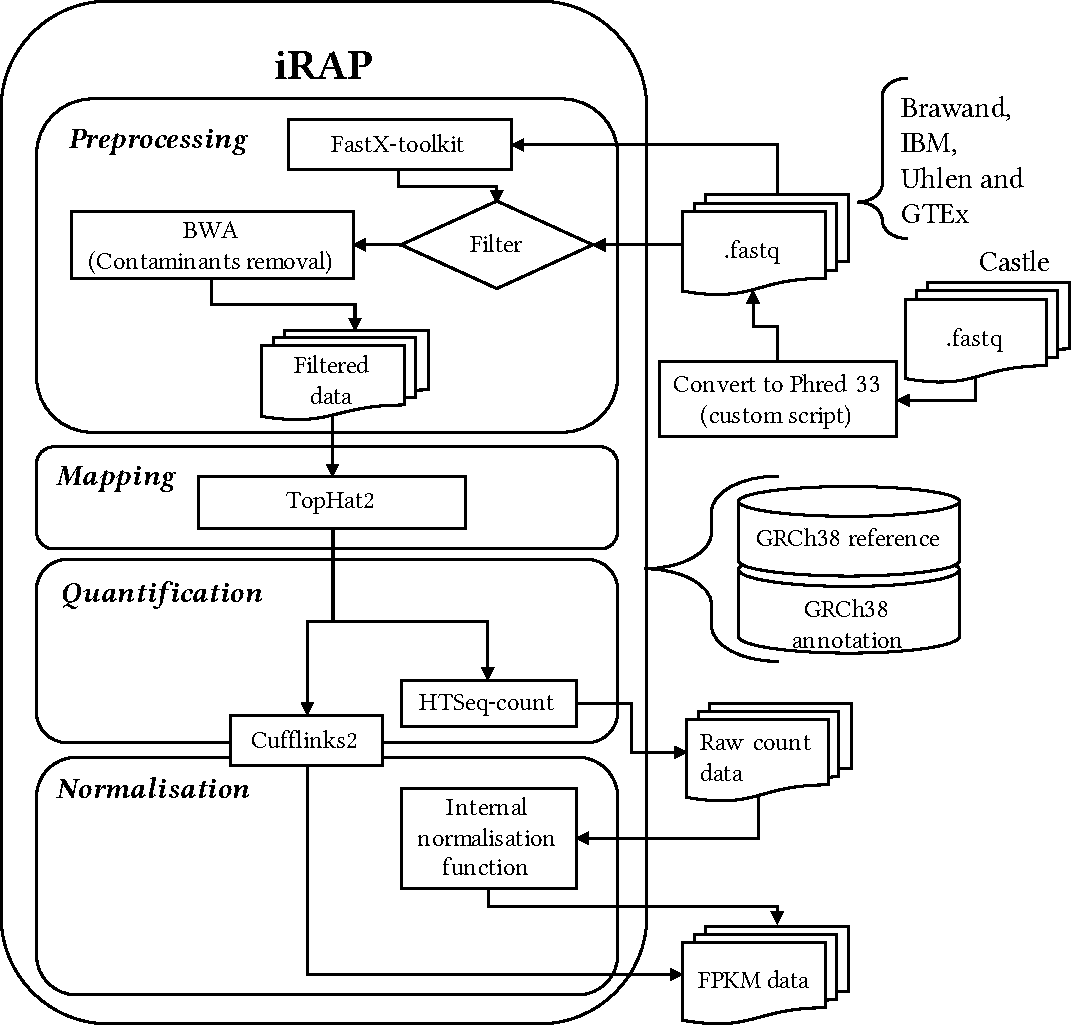
\includegraphics[scale=0.75]{datasets/pipelineTrans1.pdf}\centering
    \caption[General steps for processing the transcriptomic
    data]{\label{fig:pipelineTrans}\textbf{General steps for processing the
    transcriptome.} The pipeline \irap\ integrates
    all the tools needed for the state-of-art
    processing of \Rnaseq\ data. The quality of the reads is checked and they
    are trimmed if needed. After removal of possible contaminant reads (such as
    \species{E. coli}), the reads
    are aligned with \toph. The gene expression is then quantified with two
    different approaches: based on the aggregation of isomers for each gene or
    simply based on the number of aligned fragment on the gene locus defined in
    the reference. \cuffl\ provides directly \FPKM\ values. \htseq\ provides
    raw counts which were normalised by an \irap\ function into \FPKM.}
\end{figure}

I downloaded and entirely processed four of the transcriptomic datasets
myself (\castle, \vt, \ibm\ and \uhlen\ data) and
\nuno\ retrieved and processed the \gtex\ dataset\footnote{As
the \Gtex\ data is involved in many projects within the \EBI\
and due to its huge amount of files (number and  size --- see \Cref{tab:Lib5DF}),
it was agreed that this would be processed centrally by one person and then
redistributed to all the other interested parties. \nuno\ had this
tremendous task.}.
In this thesis,
I present results computed on the quantification of these
five datasets which have been processed through the same identical pipeline.

\begin{table}
\centering
\caption[Technical description of the 5 transcriptomic datasets]{%
\label{tab:Lib5DF}\textbf{Technical description of the five transcriptomic
    datasets}\\\footnotesize{I processed all the datasets except the one in
    \textit{\color{darkgray}italic}.\\
    For the Brawand dataset, I only included and processed the \species{Homo sapiens} part.}}
\begin{tabular}{@{}cccccc@{}}
\toprule
Dataset & \begin{tabular}[c]{@{}c@{}}Participant\\number\end{tabular} &
\begin{tabular}[c]{@{}c@{}}Library\\number\end{tabular} &
\begin{tabular}[c]{@{}c@{}}File\\number\end{tabular} &
\begin{tabular}[c]{@{}c@{}}Total size of\\the fastq\\raw files (GB) \end{tabular}&
    \begin{tabular}[c]{@{}c@{}}Mean number of\\biologic samples per\\tissues
    [min;max]\end{tabular} \\
\midrule
Castle        & 10    & 11    & 11    & 58    & 10 (mixture)    \\
Brawand       & 18    & 21    & 23    & 111   & 2.8  [2;3]      \\
{\small Illumina Body Map} & 16    & 36    & 48    & 1,004  & 1 \\
Uhlén         & 122   & 200   & 400   & 1,851  & 3.81    [2;11] \\
    \textit{\color{darkgray}\Gtex\ (v4)}  &
    \textit{\color{darkgray}551}  & \textit{\color{darkgray}3,276}  &
    \textit{\color{darkgray}6,552}  &
    \textit{\color{darkgray}$\sim$ 50,000}  & \textit{\color{darkgray}60.67 [4;214]}\\
\bottomrule
\end{tabular}
\end{table}

\subsubsection{Data retrieval and preparation}

I retrieved the human raw data of each dataset from \gls{ArrayExpress} and
\gls{ENA} through their identifier (see \crefp{sec:rnaseq-data}). After we
received our access approval, \nuno\ retrieved \Gtex\ data from
\gls{dbGaP}.

While most of the raw files can be used as they are, an additional step is
needed for the \castle\ files. Indeed these files are using an older
\fastq\ format that is non-compliant to the most accurate and recent tools used
for this thesis.
As it is a simple matter of changing the quality score scale
(see \cref{sec:PhredScore}),
I converted these files to \gls{Phred}$+33$ \fastq\ files with a
\emph{\gls{Perl}} script (see~\Cref{code:fastq}).

\subsubsection{Genome and annotation reference}

I collected and processed the datasets through an extended period of time.
Hence, for a subset of them,
I produced many intermediate sets of results based on the \hg{37.p12}
(and later \hg{37.p13}) human reference genome and the latest available
\gls{Ensembl} gene set annotation (73, 74 or 75) at that time.
In fact, the quality of each new annotation update is
generally greater than its predecessor\footnote{Although,
it is not unusual to have gene or transcript additions based on new studies
that are then removed (or fused to another) in a later version.
}.

As the \gtex\ data was processed with \hg{38.p1} and \ens{76}, that led me
to reprocess all the other four \Rnaseq\ datasets for the sake of consistency and
to avoid more biases~\mycite{h38vsh37}. Thus, unless indicated
otherwise, the results presented in the current work are
based on the \hg{38.p1} human genome reference and the \ens{76} gene set annotation.


\subsubsection{Data processing}

In the early stages of my research, I was processing each of the different steps
sequentially and semi-manually with the help of custom made scripts. While the
\EBI\ \gls{cluster} greatly facilitated the handling of the numerous files,
the task remained quite tedious.
Additionally,
the scripts I wrote would need a fair amount of work to achieve general
reproducibility on other platforms.

Fortunately, \nuno\ developed
an \enquote{integrated RNA-seq analysis Pipeline}:
\softFoCi{\irap}{https://nunofonseca.github.io/irap/}{Fonseca2014-si}.
This tool allows the automation of the typical
state-of-the-art and optimised workflow to study
\Rnaseq. It takes full advantages of the capacities provided by computer clusters.
Thus, I switched from my original set of scripts to \irap\
to improve my workflow without changing any step or parameter.

Besides the usual input files (raw \Rnaseq\ files and genome/annotation
references), \irap\ needs a configuration file that precisely describes the
dataset (its design and technical features) and, if needed, specific parameters
to use.
To provide full reproducibility,
each version of \irap\ is shipped with
its own set of third-party version-defined tools and default parameters.
Thus, apart from remarkably speeding up the data processing,
\irap\ also ensures the protocol integrity
across the five transcriptomic datasets I use
in my thesis regardless of who runs the pipeline.

Each of the transcriptomic datasets is the product of the same version of
the \irap\ pipeline (development version 0.6.3b) and set of parameters. As the
default parameters of \irap\ are tuned for human Illumina paired-end data,
I only have to define a few of them. Hence, the quality and contamination checks,
and the filtering and trimming of the reads are done following the default options
of \irap.

\minisec{Quality assessment, trimming and filtering}
\irap\ uses internally
\softFo{FastX toolkit}{http://hannonlab.cshl.edu/fastx\_toolkit/} (0.0.13)
to perform the
assessment and the trimming. The usual uninformative and ambiguous reads
(see \Crefu{subsub:trim})
have been discarded as were any with an overall quality score below
a threshold of 10.

As reported in the \Crefu{subsub:sequencing}, as the base calling progresses,
the quality of the call decreases.
On another note, some tools (mappers in particular) need
all the reads to be trimmed to the same length. \irap\ optimises the compromise
between the purity and the length of the reads to avoid more errors or
biases due to smaller reads~\mycite{Trimwisely} by trimming at most 15\% of the
original length while discarding more reads if necessary to maximise the length.

Reads that could be assigned to a likely contamination source, here
\species{Escherichia coli} (as I work with \species{Homo sapiens}),
are also discarded. A non-splice aware mapper,
\softFo{Bowtie}{http://bowtie-bio.sourceforge.net/}~(1.1.1)~\mycite{Bowtie}
maps all the reads to the
contaminant genome and all the reads mapping perfectly and unambiguously are
discarded.

\minisec{Mapping}
I mapped the reads to the genome (\hg{38.p1})
and the transcriptome (\ens{76} gene set annotation)
with \irap's (0.6.3b) proposed default splice-aware mapper
\hFo{\toph}{https://ccb.jhu.edu/software/tophat/index.shtml}
(2.0.12)~\mycite{tophat2}
with its set of default predefined arguments.
Indeed, \toph\ can handle reads from many organisms
by fine-tuning the parameters (\eg\ number of mismatches or indels to tolerate),
but the default parameters are adjusted for normal human.

\minisec{Quantification and Normalisation}
While \Rnaseq\ can be used to identify (and discover) \gls{RNA}
isoforms, I have focused my thesis on the gene level expression. Indeed, current
annotations and knowledge are still lacking in the reasons and
external conditions that impact the expression of a specific isoform over the
others. In addition, criticisms have been raised on the accuracy of distinction
between them~\mycite{tamaraRNA,ernestRNA}. Normalising gene expression
presents more challenges than specific transcript expression,
for instance the definition of the gene length may be different
from one lab to another.

In the framework of this thesis,
when I have to use a gene length for a computation,
I use the identical gene length definition as found in
\irap\ and \egxa.
Thus, as shown on \Cref{fig:Genelength-collapsedExons} the gene
length is defined as the sum of the lengths of all its \emph{collapsed} exons.

\begin{figure}
    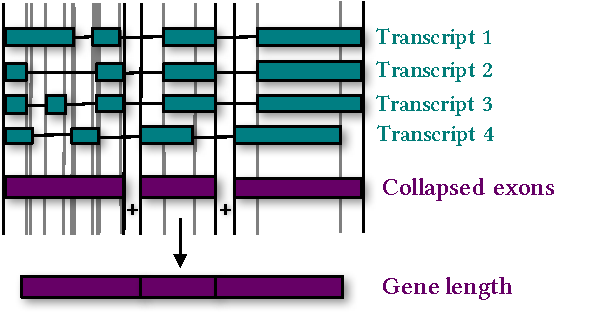
\includegraphics[scale=0.8]{datasets/collapsedExonsLinLib.pdf}\centering
        \caption[Gene length is equal to the sum of the lengths of all its collapsed
        exons]{\label{fig:Genelength-collapsedExons}\textbf{Gene length is equal
        to the sum of the lengths of all its collapsed exons.} Though,
        this method lacks  complete accuracy, it provides a sufficient estimation
        of the gene length for an efficient normalisation regarding the length bias.
        The coordinates for the 5' and 3' ends of each exon is extracted from
        the annotation and they are collapsed together. This \emph{gene length}
        is unaffected by incorrect attribution of a fragment to a
        specific transcript when there are many possible options.}
    \end{figure}

As mentioned in \Crefu{subsub:norm}, I used two different popular tools based on
different strategies to estimate
gene expression levels:
\hFo{\cuffl}{https://cole-trapnell-lab.github.io/cufflinks/manual/}
(2.2.1)~\mycite{cufflinks}
and \hFo{\htseq}{https://htseq.readthedocs.io/}
(0.6.1p1)~\mycite{htseq} (with the \texttt{intersection non-empty} mode).
These tools are also integrated in \irap.

For \cuffl, I used the mode where the multi-mapped reads are probabilistically
assigned depending on the coverage of each mapped locus. In addition,
\cuffl\ provides normalised gene expression levels by aggregating their
corresponding normalised isoform expression levels. \cuffl\ uses the
\cref{eq:rpkm-fx} to normalise isoform expression levels. The length of the
isoforms are extracted from the reference.

On the other hand, \htseq\ provides only \emph{raw} counts for the feature of
interest. \irap\ provides an internal \FPKM\ normalisation function that
is an implementation of the \cref{eq:rpkm-fx}. As I requested \htseq\ to work at
gene level, this formula requires gene lengths which are computed with the
aforementioned method.

All the configuration files I created for this thesis may be found at
\addressToirapConfFiles.

As the paired-end set of the \ibm\ data was presenting an overall better
quality than its single-end counterpart,
I only include \ibm{}'s paired-end data for the remaining of the thesis.

\subsection{MS data processing}

After retrieval of the data from \gls{Pride} and \gls{Proteomicsdb},
\james\ reprocessed the three proteome \ms-based datasets.
\Cref{fig:pipelineProt} illustrates the pipeline that processed the three
datasets in a consistent and optimal manner. I summarise this protocol
in \Crefp{fig:pipelineProt}{}
and in the following \cref{subsub:spectralProcessing,subsub:seqDBseeking,%
subsub:spectralIDDBsearch,subsub:resultsFiltering}.
See~\citet{Wright-2016,Weisser2016-pipeline} for more details.

  \begin{sidewaysfigure}
      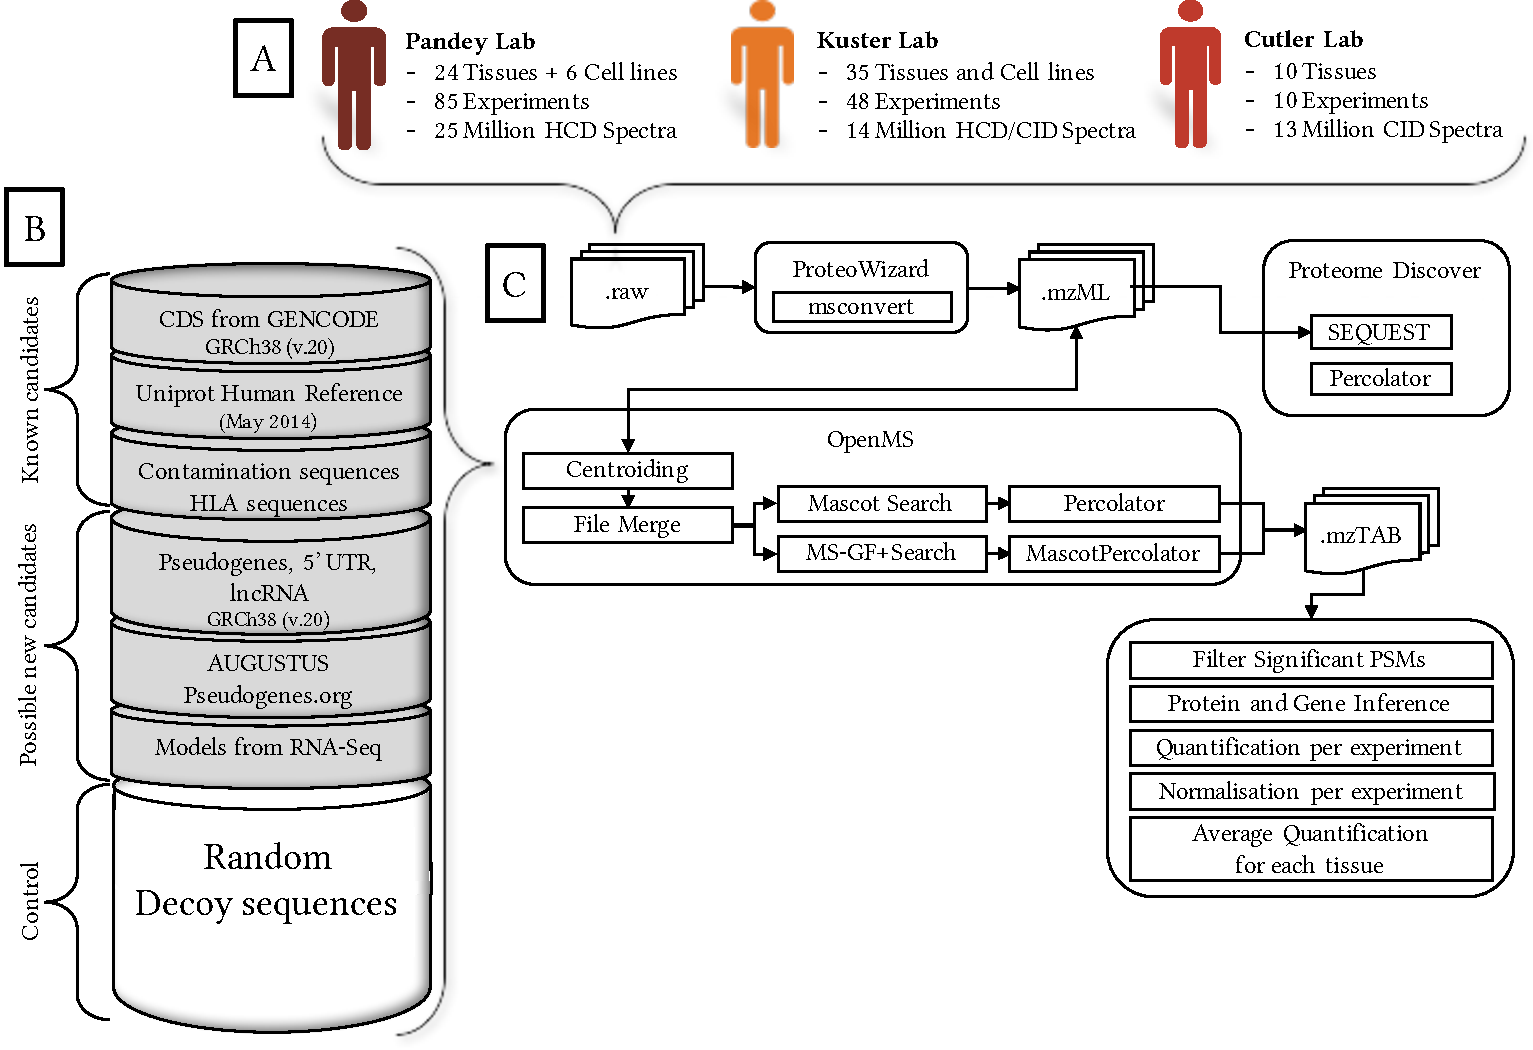
\includegraphics[scale=0.75]{datasets/pipelineMS-2.pdf}\centering
      \caption[General steps for processing the proteome
      data]{\label{fig:pipelineProt}\textbf{General steps for processing the
      proteome.} [Adaptation of courtesy materials from \james].\\
      (\textbf{A}) The three datasets have been processed through the
      same pipeline. I only use their normal tissues samples and I also discard
      the cell lines. (\textbf{B}) Extensive sources of protein sequences were
      used for the search database, including prediction of novel proteins.
      Contamination and decoy sequences were also included to allow for \gls{FDR}
      estimation. (\textbf{C}) State of the art workflow was used to process the
      \ms\ data from raw files.
      This workflow combines multiple \ms\ search engines and
      post-search evaluation tools. Results were filtered by peptide length,
      \gls{FDR}, \gls{PEP} and agreement between the multiple search algorithms.
      \\\NB\ There is no relation between the real size of
      the database parts and their representation.}
  \end{sidewaysfigure}

\subsubsection{Spectral processing}\label{subsub:spectralProcessing}

The \soft{msconvert} module of \softFull{ProteoWizard}%
{http://proteowizard.sourceforge.net/}{ProteomeWizard}{v3.0.6485}
converted all the files to the standard format mzML.\@
\softCi{TOPP}{Topp} from
\softFull{OpenMS}{https://www.openms.de/}{openMS2016}{pre-v2.0 development build},
processed the raw spectra. Notably, \soft{PeakPickerHiRes} which centroids them
and \soft{FileMerger} that merges the ones from the same fractionated experiments.

\subsubsection{Sequence database creation and searching preparation}%
\label{subsub:seqDBseeking}

The target sequence database is a critical element of the \ms\ pipeline and thus,
\james\ has carefully designed it.
It combines six different parts, three based on
known protein sequences and three other covering possible new protein candidates.

The known sources include the complete human \hg{38} (v.20) \gls{CDS} translated
sequences from \gls{GENCODE}; the human reference proteome from
\gls{Uniprot}\footnote{%
\gls{Uniprot} --- \Href{http://www.uniprot.org/}}~\mycite{UniProt2017}
(in its May 2014 version); common contamination protein
sequences\footnote{Contamination sequences ---
\Href{http://maxquant.org/contaminants.zip}}
and \gls{HLA} sequences\footnote{\gls{HLA} sequences ---
\Href{https://www.ebi.ac.uk/ipd/imgt/hla/download.html}}.

The sources for potential
novel proteins included a selection of non-coding gene sequences (including
pseudogenes, \gls{lncRNA} and untranslated regions) from \gls{GENCODE}
\hg{38} (v.20); prediction of novel sequences with
\softFoCi{\mbox{AUGUSTUS}}{http://bioinf.uni-greifswald.de/augustus/}{Stanke2004};
a set of two-consensus predictions (December 2013)
from \softFoCi{Pseudogene.org}{http://pseudogene.org/}{pseudogenesOrg}
and three-frame translated \Rnaseq\ transcript sequences.
These translated sequences include models
built on \ibm\ by \gls{Ensembl} and by the Kellis lab in addition with
models built on different \gls{ENCODE} cell lines by Caltech and CSHL\@.
%Precautions were taken with the handling of the overlapping regions
%and with the sequence three-frame translations.

\softFo{Mimic}{https://github.com/percolator/mimic} generated the randomised
decoy sequences (equal sizes of the target database sequences).
The different databases were then merged together.
It is represented on \Cref{fig:pipelineProt}{\footnotesize B}

To account for the isobaric peptides, all isoleucine (I) residues were
converted to leucine (L) before the search and then after the search all leucine
(L) residues were converted to (J)\footnote{As J is one of the letter
from the Latin alphabet that do not map to any amino acid.}
to avoid later misconceptions.
In summary, the known coding portion of the tryptic peptides sequences represents
787,587 peptides and the novel portion provides an additional 4,211,835 peptides.

%\NB\ For each peptide sequence, there is a unique identifier,
%an associated source database
%and, when available, the corresponding gene locus.

\subsubsection{Spectral identification and database search pipeline}%
\label{subsub:spectralIDDBsearch}

\Cref{fig:pipelineProt}{\footnotesize C} describes the overall workflow used by
\james\ to quantify the protein abundance in each tissue. As mentioned in
\Cref{seg:moreAlgoisbetter}, workflows involving several algorithms produce
better results. \soft{Mascot} Server~(v~2.4--- Matrix Science)~cluster produced
a first search on the mzML files submitted through \soft{MascotAdapterOnline}
(part of \soft{TOPP}). In parallel, \james\ also used  \soft{MS-GF~$+$~Search},
which involves the run of \soft{MS-GF~$+$}~(v. 10089)~\mycite{Kim2014-nj}.
\soft{MascotPercolator}~(v~2.08)~\mycite{Brosch2009-xq,Wright2012-od}
optimised and rescored the results from \soft{Mascot} and
\soft{msgf2pin/Percolator} (v~2.08\textminus1)~\mycite{Granholm2014-cw} optimised
the results from \soft{MS-GF~$+$}.
Finally, \soft{SEQUEST}~\mycite{Eng1994-eq} and
\soft{Percolator}~\mycite{Spivak2009-zd} performed a search in a
\soft{Proteome Discoverer}~(v 1.4 --- Thermo Scientific) workflow.

The different workflows used common stringent parameters for all the database
searches:
the precursor tolerance was set to 10 \gls{ppm};
fragment tolerance for \gls{HCD} spectra to $0.02$ \gls{Da} and
to $0.5$ \gls{Da} for \gls{CID} spectra;
the allowed missed cleavages were limited to $3$;
several amino acid modifications were
also used for the research (see~\citet{Wright-2016}).

The search results were converted into mzTab formatted files and uploaded along
with the mzML spectra and FASTA search database to \Pride{PXD002967}.

\subsubsection{Results processing and filtering}\label{subsub:resultsFiltering}

Custom Perl scripts parsed, merged and filtered the results of each search engine
so that every \gls{PSM} had the same identification in at least two of the three
search engines.
In each case, the least confident \gls{PEP} (\ie\ the highest) was retained.

The \glspl{PSM} were then filtered to only keep matches to the three following
criteria:
\gls{q-value} less than or equal to $0.01$ (\ie\ 1\% \gls{FDR});
% $\leq 0.01$
a \gls{PEP} inferior or equal to 0.05 and
a peptide length superior or equal to 7 amino acids.
\glspl{PSM} matching contaminant or decoy sequences were also removed.

The resulting list of peptides was then used to infer the proteins with
a simple approach.
Protein clusters are created based on the common matching non-null set of peptides,
\ie\ each protein cluster has at least one unique peptide.
Then, the \gls{GENCODE} \gls{CDS} and \gls{Uniprot} accession were mapped back to
\gls{Ensembl} identifiers.
The genes that were matching at least 3 unique peptides were kept for the
remaining of the analysis while the others were discarded. Protein clusters
matching several gene identifiers or failing the \emph{unique peptide} rule were
discarded. (The list of the discarded clusters is different for each of the
proteome datasets.)

The quantification (and normalisation) of the retained proteins were computed
with the Top3~(\gls{IBAQ}) approach for each experiment.
When there were more than one experiments per tissue, the final quantification
values are the average across all the experiments of each tissue.

Compared to the original \pandey\ study, fewer proteins were quantified, but
the results are congruent to other previous studies on the range of detection
and quantification of \gls{LC-MS/MS}. The quantifications were released along
our paper~\mycite{Wright-2016} and the reanalysis of the \pandey\ data was
also released through \egxa\ under the accession: E\textminus{}PROT\textminus{}1.

\section{Discussion and Conclusion}

In this chapter, I introduced the five transcriptomic and three proteomic normal
human tissues datasets on which I based my thesis.
I described how both the transcriptomic and the proteomic datasets have been
reprocessed from raw files with state-of-the-art unified pipelines
which are also using the same genome build and annotation references in the
final processed version.

As mentioned before,
I have produced a subset of the transcriptomic datasets
with the previous human reference genome~(\hg{37}) and
three different \gls{Ensembl} gene set annotations (73, 74 and 75).
I have run many of the analyses of \Cref{ch:expression,ch:Transcriptomics} on
these data.
While the results may vary for individual genes,
the overall outcomes are congruent hence
supporting the robustness of the findings presented in this thesis.
In addition, the products of these pipelines (either for the \Rnaseq\ or the \ms\
data) are in agreement with the original studies findings ---
except for~\citet{PandeyData}.

While we are in the era of \emph{data deluge} and \emph{big data},
the number of tissue overlaps for independent normal human studies is surprisingly small
--- see \Crefp{fig:VennStudiesT}.
Most of these datasets have been (and will be) referenced through
many papers for comparison (or as control) purposes;
hence, it is essential to assess the soundness of these practices by assessing
the consistency between these datasets.


\chapter{About expression visualisation, correlation and clustering}
%\chapter{More quality checks and data preparation}
\label{ch:expression}

\begin{comment}
\setlength{\epigraphwidth}{\textwidth}%0.6
\setlength{\epigraphrule}{0pt}%0.1
\epigraphhead[70]{%
\epigraph{[..] 80\% of the data analysis task is spent on cleaning and
understanding the data.}{\cite{Dasu2003-bg}}%
}
\end{comment}

As a first step towards the meta-analyses\footnote{Across transcriptomes,
across proteomes and then across transcriptomes/proteomes.},
I have opted for a semi-empirical approach to determine
a consensus set of methods and parameters on each individual study
before applying them across all the datasets in the further chapters.
This strategy has also allowed me
to estimate the data overall quality per dataset and to tidy them appropriately.

I report quality checks in \Cref{ch:datasets}
that happened before the processing of the data.
Those quality assessments are rather technical\footnote{Is it true signal
or noise?
Are all the nucleotides called?
Is it a true identification or a \gls{FDR}?~\ldots}.
In the present chapter, I describe post-processing quality (or sanity) checks
that examine higher (and fuzzier) aspects, \eg:
%\KOMAoptions{parskip=never}
\begin{itemize}[topsep=0pt,nosep]
    \item Possible outliers in the data
    \item Systematic and unsystematic \emph{batch effect} within each study
    \item Adequacy of data, concepts and statistical models
\end{itemize}
%\KOMAoptions{parskip=half*}
Even if every aspect may not be addressed or corrected the
final results and their interpretations are more solid.

\section{Visualisation of expression data}

Visualising the data first is a very effective method towards adequate analyses
and more pertinent results by uncovering
the detection of underlying structures and possible unwanted artefacts.

\subsection{Distribution plots}\label{subsec:distribPlot}

In the literature, the distribution of expression values are frequently
visualised on a log-scale ($\log_{2}(x)$).
\Cref{fig:distribPlot} and~\Cref{fig:distribPlot_noLog2} illustrate how
this scaling improves the readability of the figure.
Furthermore, the log-scale allows to transform count data to continuous
while smoothing the global distribution shape towards a normal distribution.
Thus, another advantage of this transformation is to conform the data
to many ready available statistical models.

\NB\ Whenever removing the null values is harmful statistically
or for correct interpretation,
I have added a common \emph{pseudocount} (equals to $1$)
to overcome the lack of definition of $\log_{2}(0)$.

\Cref{fig:distribPlot} shows that all \gls{RNA} samples present a similar
profile on this $\log_{2}(x+1)$ scale:
a pic near $0$ for the lowly (and not expressed genes) and a long-trailing tail.
The bulk of the expressed genes on this scale is below $6$ (\ie\ below 63 \FPKM).
Besides, in \Cref{fig:densityUhlen_log2}, we can observe that the general expression
of the pancreas is shifted towards the left in comparison of the other tissue.
This is probably an artefact as this shift is absent in the other pancreas
tissue samples of other transcriptomic datasets.

Aside from the \pandey\ data (\cref{fig:densityPandey_log2}),
the expression of the proteins is more heterogeneous
(in particular \cutler\ data, see \cref{fig:densityCutler_log2}).
This is concordant to the more disparate and various techniques involved in
the proteomic sample preparation (see \cref{subsec:ProtSampPrep}).


\begin{figure}
    \centering
    \begin{subfigure}[b]{0.35\textwidth}
        \centering \includegraphics[width=\textwidth]{expressed/density_Log2/castle.pdf}
        \caption{Castle}\label{fig:densityCastle_log2}
    \end{subfigure}%
~%
    \begin{subfigure}[b]{0.35\textwidth}
        \centering \includegraphics[width=\textwidth]{expressed/density_Log2/vt.pdf}
        \caption{Brawand}\label{fig:densityBrawand_log2}
    \end{subfigure}

    \begin{subfigure}[b]{0.35\textwidth}
        \centering \includegraphics[width=\textwidth]{expressed/density_Log2/ibm.pdf}
        \caption{Illumina Body Map}\label{fig:densityIBM_log2}
    \end{subfigure}%
~%
    \begin{subfigure}[b]{0.35\textwidth}
        \centering \includegraphics[width=\textwidth]{expressed/density_Log2/uhlen.pdf}
        \caption{Uhlen}\label{fig:densityUhlen_log2}
    \end{subfigure}

    \begin{subfigure}[b]{0.35\textwidth}
        \centering \includegraphics[width=\textwidth]{expressed/density_Log2/gtex.pdf}
        \caption{Gtex}\label{fig:densityGtex_log2}
    \end{subfigure}%
~%
    \begin{subfigure}[b]{0.35\textwidth}
        \centering \includegraphics[width=\textwidth]{expressed/density_Log2/cutler.pdf}
        \caption{Cutler}\label{fig:densityCutler_log2}
    \end{subfigure}

    \begin{subfigure}[b]{0.35\textwidth}
        \centering \includegraphics[width=\textwidth]{expressed/density_Log2/kuster.pdf}
        \caption{Kuster}\label{fig:densityKuster_log2}
    \end{subfigure}%
~%
    \begin{subfigure}[b]{0.35\textwidth}
        \centering \includegraphics[width=\textwidth]{expressed/density_Log2/pandey.pdf}
        \caption{Pandey}\label{fig:densityPandey_log2}
    \end{subfigure}
    \caption{Profile of expression across the transcriptome (protein coding
    genes only) and proteome datasets}\label{fig:distribPlot}
\end{figure}

\subsection{Scatter plots}

\cite{anscombe} created four datasets (see \Cref{fig:Anscombe})
which share similar descriptive statistics to show the importance
of data visualisation even through a simple scatter plot.
He demonstrated that checking the datasets graphically with scatter plots
allows to quickly detect outliers and roughly estimate
the relationship between two variables.
Even a non-linear but strong relationship is promptly highlighted
(\eg\ top right corner of~\cref{fig:Anscombe}).

\begin{figure}
    \centering
    \begin{subfigure}[b]{0.48\textwidth}
        \centering 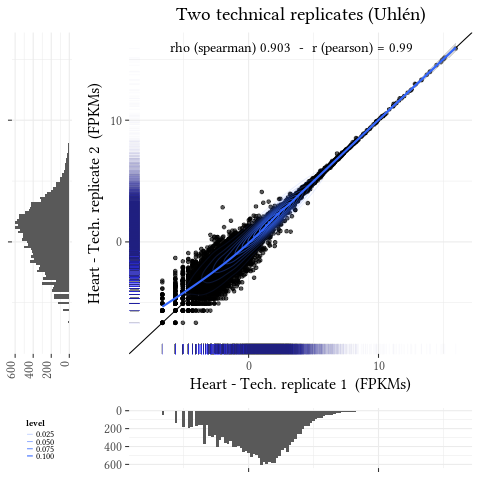
\includegraphics[width=\textwidth]{expressed/RepTechscat_heart.pdf}
        \caption{Technical replicates (Heart)}\label{fig:scatTechRep}
    \end{subfigure}~%
    \begin{subfigure}[b]{0.48\textwidth}
    \centering 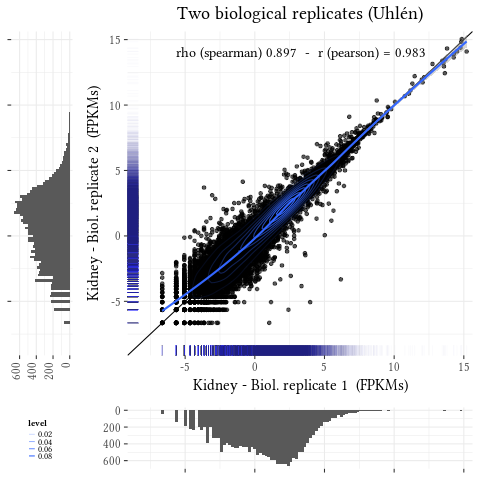
\includegraphics[width=\textwidth]{expressed/RepBiolscat_kidney.pdf}
        \caption{Biological replicates (Kidney)}\label{fig:scatBiolRep}
    \end{subfigure}
    \caption{Examples of scatter plot for replicates from \uhlen\
    (transcriptome)}\label{fig:scatEg}
\end{figure}

\Cref{fig:scatTechRep} illustrates how very lowly expressed \gls{RNA}
diverge even in technical replicates.
Biological replicates, within a same dataset,
may present very close profiles though with a greater spread
as showed in \Cref{fig:scatBiolRep}.


\section{Main statistical approaches}

Due to the general normal distribution shape of the gene expression levels,
I computed correlation coefficients to assess the similarity of the replicates
intra and inter studies.

\subsection{Correlation}
%Cum hoc ergo propter hoc

Correlation coefficients are a measure of the statistic dependence between two
continuous variables\footnote{In the context of this study: either expression
levels of a given gene across samples/tissues or expression levels of all genes
\emph{between} two samples or tissues} (\eg\
$X$ and $Y$) and always ranges within $[-1,1]$ (see also \cref{sec:CorrMore}).

The correlation coefficient is computed by pairwise comparing observations
between the two variable. Most implementation methods
will manage an unbalanced number of observations by excluding the incomplete pairs.
To ease the interpretation I preferred to filter the data \latin{a priori}
myself; I only kept expression values \emph{effectively observed}
in all the datasets (see~\cref{sec:ExpressedOrNot}).

Among the several methods available to compute the correlation coefficient,
I tried both the Spearman and the Pearson correlations
(see respectively \cref{subsec:SpearmanCor} and \cref{subsec:PearsonCor}).

\begin{table}[]
\centering
\caption{Correlation coefficients between \Rnaseq\ replicates}
\label{tab:repCorr}
\begin{tabular}{@{}cccc@{}}
\toprule
Tissue & Replicates type & Pearson Correlation & Spearman Correlation \\ \midrule
\vt\ & Biological & 0.90 $[$0.45;1$]$ & 0.93 $[$0.80;0.99$]$ \\
\gtex\ & Biological &  0.75 $[$0;1$]$ & 0.93 $[$0.06;0.99$]$ \\
\uhlen\ & Biological & 0.81 $[$0.15;1$]$  &
0.95 $[$0.70;0.99$]$ \\
       & Technical & 0.99 $[$0.68;1$]$ & 0.99 $[$0.92;1$]$\\
\bottomrule
\end{tabular}
\end{table}

\Cref{tab:repCorr} presents the Pearson and Spearman correlation coefficients
for the technical replicates for \uhlen\ study and
the biological replicates within \vt, \gtex\ and \uhlen\ studies.
Averagely the correlation coefficients are high either for the technical or
the biological replicates.
Technical replicates present higher Pearson correlations,
while biological replicates have higher Spearman correlations.
\gtex\ study presents the same average correlation coefficients but extreme range.
This may be explained by great strong batch effect as the samples were collected
and sequenced at different time by different laboratories.

\subsection{Clustering analysis}

As we know the tissue type for each sample of each dataset,
we may debate that supervised analyses can be more informative.
However, they would involve proper corrections for batch effects and
other technical biases for each dataset.
This is challenging as that often requires more knowledge than the available one
through the repositories.
In \Cref{ch:datasets}, we have seen it is also unwise to rely solely on the
normalised data provided by the original authors\footnote{Eventual bias
corrections in \Rnaseq\ vary according to planed downstream analyses and
proteomic data is hard to handle and two processing pipelines may rather give
quite different results (see~\Cref{ch:proteomics}).}.

To assess the consistency of the quantification across the different datasets,
in particular for \Rnaseq,
I picked a widely used and unsupervised method for gene expression studies:
a clustering analysis.
This method uncovers possible hidden
structures within the data, therefore,
it is well designed for exploratory studies.
I can thus confirm if samples are more alike either due to their
biological or their study origins.

In general, we expect biology to be a better predictor when we only consider
data from either transcriptome or proteome. Even more so, if the
identification technology and the quantification workflows are
consistent. Yet, a technical predictor can not be excluded straightforwardly.
Indeed, most transcripts (in particular \mRNAs) are expressed in many tissues
and two random tissues share about 60 to 90\% of their pool of
\mRNAs~\mycite{ramskoldan:2009,UhlenGastro}.
Coincidentally, on the proteome side,~\cite{PandeyData}
estimate that 75\% of the mass of a cell is due to ubiquitous proteins and
\cite{KusterData} estimate that about 10,000
to 12,000 proteins are ubiquitously detected, which represent about 60 to 75\%
of the proteins that they identified per tissue. Thus, if the variation of
expression are too subtle from one tissue to another, a strong sample collection
or data processing bias may hide any relevant biological signal.

There are many available approaches and algorithms for clustering analysis.
I~chose a (bottom-up) \emph{hierarchical} clustering (a.k.a.\
\emph{connectivity-based} clustering).

This sort of clustering is broadly used in gene expression studies as it is
embryologically\footnote{Or evolutionary, when different species are compared}
pertinent\footnote{The whole organism develops from
an original single cell.}. The data is portioned in an extensive hierarchy:
each cluster merges with another at a certain distance.
In practice, each sample starts in its own cluster and then
by iteration, each cluster is merged with its nearest one.
The method has two parameters: the distance and the linkage method.
Debate is still going on how to pick these parameters (for more details
see~\mycite{Jaskowiak2014}).

The distance measures the dissimilarity between two samples and one common
approach is to calculate the subtraction result of
the correlation coefficient from $1$ (hence, a greater similarity between the two
samples means a smaller distance). As previously, I have also used both Spearman
and Pearson correlation methods.

The linkage parameter specifies which part of each cluster is used as reference
for computing the distance between the clusters. There are many methods and after
trying several, I have arbitrary selected the one that divides the most accurately
the samples by their tissue source across the different datasets.
In fact, I noticed that the Ward's method~\mycite{Ward1963}
was the best for this task and was outperforming the complete-linkage method.
Indeed, this later method was used in~\mycite{Uhlen2014}
(first release of the \uhlen\ dataset) where
the original authors have to discard a few samples as they were clustering
incoherently in regards of their biological nature.
However, the Ward's method allows to conserve all the samples for the analysis
as long as another bias source is corrected (see \cref{subsec:mito}).


\section{Reducing obvious bias sources}

Many non-trivial methods correct for the skewness presents in
\Rnaseq\ and \ms-based proteome global expression distributions
and for other possible bias sources.
However, it may be complex to assess the biological relevance of those corrections.
Hence, while it may be better to correct for every bias in principle,
in the context of this thesis, this is a smaller concern as I am interested into
consistent traits across the datasets that may be consolidated into a reference.
Nonetheless, prior to the analysis and while its early stages,
I found a few easily avertible biases that I describe hereinafter.


\subsection{Mitochondria issue}\label{subsec:mito}

Gene expression levels of mitochondria can report very useful information,
\eg\ the stress level of a cell in a single cell experiment~\mycite{Ilicic2016}.
However, it is unwise to keep them for a bulk analysis, particularly when
comparing different biological sources.
Indeed, it is very hard to properly normalise their expression.
It involves knowing the amount of mitochondria in the studied samples.
I have decided to remove them from the analysis as they skew anything relying
on correlation.
In fact, there are always mitochondrial genes among the highest expressed genes
and they usually dominate manifolds the expression of the other genes.

Removing the 37 mitochondrial genes from the bulk of expressed genes
(above 10,000 protein coding genes) produces more defined clusters as showed on
\Cref{fig:MitoNomito} (see also \Cref{ExpGenePcoding1_withMito} in comparison
of \Cref{ExpGenePcoding1}).

\begin{figure}
    \centering
    \begin{subfigure}[b]{0.79\textwidth}
        \centering
        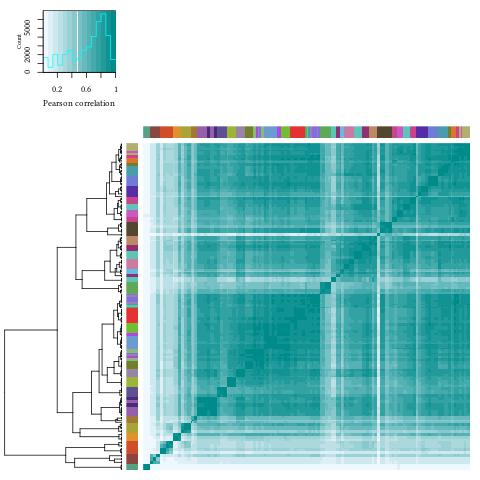
\includegraphics[width=\textwidth]{expressed/Uhlen_noLog_mito_htseq.jpeg}
        \caption{With the 37 mitochondrial genes}\label{fig:withMito}
    \end{subfigure}

    \begin{subfigure}[b]{0.79\textwidth}
        \centering
        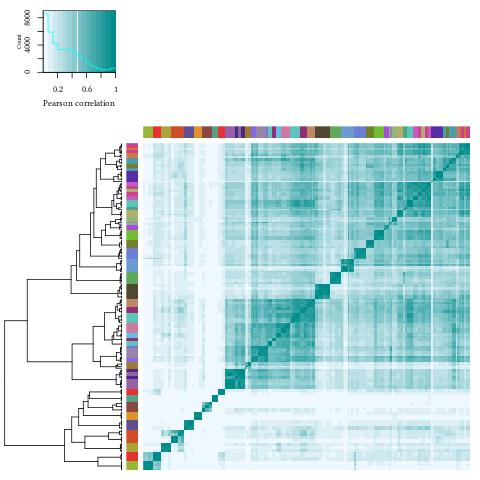
\includegraphics[width=\textwidth]{%
            expressed/Uhlen_noLog_NoMito_htseqPearson.jpeg}
        \caption{Without the mitochondrial genes}\label{fig:NoMito}
    \end{subfigure}
    \caption[Clustering of the biological samples of \uhlen\
    dataset based on the Pearson correlation]{\label{fig:MitoNomito}\textbf{Clustering
    of the biological samples of \uhlen\ dataset based on the Pearson correlation}
    --- all expressed genes are included.}
\end{figure}


\subsection{Protein coding genes}\label{subsec:protcodingOnly}
I have focused my analyses on the \mRNAs\ (\ie\ \glspl{RNA} that have a
biotype described as \emph{protein coding} in \ens{76}).

In addition of the obvious reason to match with the proteomic data,
most of the transcriptomic data is the produce of poly-A selected protocols
(see \cref{msec:polyA}).
Thus, aside of the \mRNAs, all the other \glspl{RNA} are off-target
and, for many of them,
their expression levels estimations may be highly imprecise.



\subsection{Expressed or not expressed}
\label{sec:ExpressedOrNot}

While it can seem as a trivial concept and might be overlook, whether a specific
molecule is expressed --- or not --- in a given condition, can actually have
an extensive impact on the results of the analyses, particularly when integrating
proteome and transcriptome together.

For example, the Pearson correlation coefficient is very
sensitive to outliers and null values. If for both samples, a vast number of
null values are recorded, this will lead to a greater similarity.
Hence, it is important that the data used for the analysis is meaningful in
its whole, \ie\ a null value has still to be an observation and translates
a lack of expression (and not a lack of observation).

\begin{figure}[!htbp]
    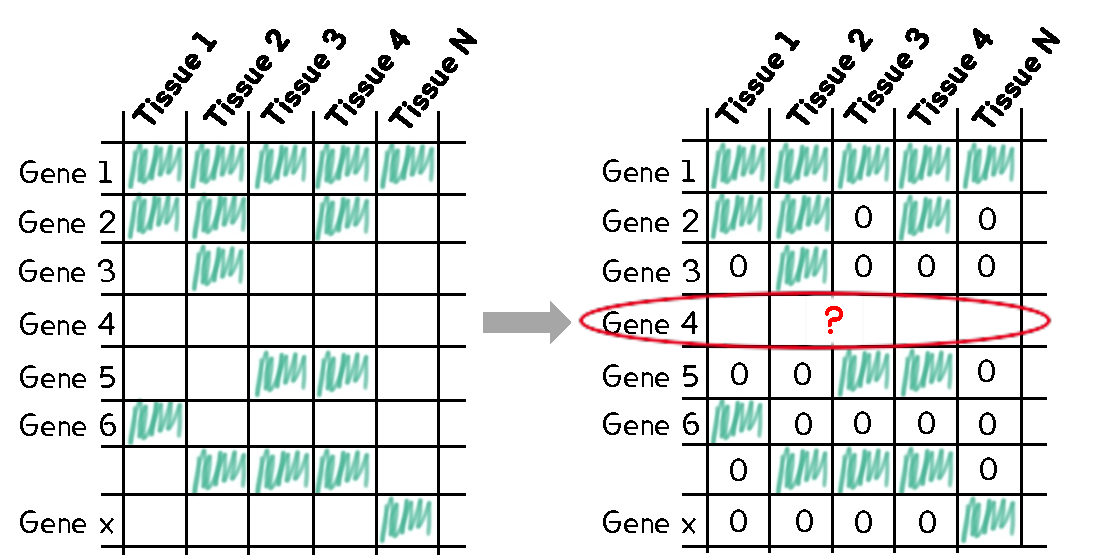
\includegraphics[scale=0.7]{expressed/expressedNotExp.pdf}\centering
      \caption[Expressed or not: several cases illustrated]
      {\label{fig:DefineExpression}\textbf{Expressed or not: several cases
      illustrated.}\smallbreak{} Genes as \emph{gene 1} are unequivocal: they have been
      detected in all the different tissues. Genes that have been quantified in
      \emph{some} of the conditions are, in principle, detectable with the
      protocol of sampling and quantification used for the assay.
      For these genes, when no signal is collected, I assume this is a true $0$.
      The genes without any quantification
      in any tissue, \eg\ gene 4, are discarded from the remaining analysis as
      I can't state
      either there are truly absent from the biological sample or it has to due
      to the protocol at use; they are \emph{undefined}. The same approach is used
      for the transcriptome and the proteome.}
\end{figure}

\subsubsection{The undefined}%\KOMAoptions{parskip=false}
\label{subsec:ExpressedOrNot-undefined}
If a protein or transcript is never found in any of the samples of a dataset,
then I considered that we can not determine if the protein or transcript was
either truly not expressed or, for any reason, was not capture while the library
preparation or the identification/quantification steps. Hence, those are
excluded from the analyses as I can not resolve precisely if this is a
technical artefact or a biological truth. This case is illustrate by the row
circled in red in~\cref{fig:DefineExpression}.

\subsubsection{Expression in a dataset}
\label{subsec:ExpressedOrNot--expDataset}
By contrast, if a protein or a transcript is expressed in some samples of the
dataset, then, whenever no expression was recorded in the other
samples, I consider that the expression of the considered macromolecule is truly
null for those samples.

\subsubsection{Expression within a sample}
Due to the technical (and biological) differences between proteomics and
transcriptomics, I use different thresholds to define the expression of a protein
or a transcript.

\minisec{Expressed protein}
On the proteomic side, I consider that a protein is expressed if it has been
identified and quantified. In other words, if the expression value of a protein
is greater than zero in a sample, I consider it as expressed.

\minisec{Expressed transcript}\KOMAoptions{parskip=half*}\label{subsubsec:exprTrans}
It is a bit more complex on the transcriptomic side as we have to account for
technical noise, but we can also expect \enquote{translational noise}~\mycite{rnaseq-2009},
\mycite{lowNoiseLimit}.
While we can empirically evaluate it for each \Rnaseq\
dataset~\mycite{ramskoldan:2009},
there is a widespread threshold used in the literature:
1 \gls{FPKM} (or \gls{RPKM}).
In fact,~\citet{Hebenstreit:2011} showed in their study
\paper{\citetitle{Hebenstreit:2011}},
that to be detected and quantified as a protein,
a \mRNA\ should at least present an expression equals to 1 \gls{RPKM}.

Hence, I have used this threshold to run (at least once) all the analyses.
As an important part of my thesis focuses on
the comparison of proteomic and transcriptomic data (see \Cref{ch:Integration}),
I have run all the analyses at least with this threshold of $1$ \gls{FPKM}.

It may worth mentioning that I have also redone parts of the analyses without
any threshold (\ie\ I use then the same definition for the \mRNAs\ than for the
proteins) or with a threshold of $5$ \glspl{FPKM}\footnote{While this threshold
may be found in the literature, it remains rather arbitrary.}.

\subsubsection{Limitation of the study}
While I may have compared the list of
undefined, expressed and unexpressed molecules
the bulk of the analyses has been done on the common expressed genes across
the datasets.

In other words, if a \mRNA\ --- or protein --- is not expressed in at least
one sample in \emph{every and each} of the datasets used for the analyses,
I then exclude it.

\subsection{Averaging tissue expression}

Finally, to avoid unnecessary skewness in the meta-analysis due to
the biological replicates unbalance across the datasets (see \cref{sec:expDesign}),
I computed a \emph{\enquote{virtual} reference} for each tissue
for the datasets that present more than one biological sample per tissue,
\ie\ \vt, \uhlen\ and \gtex\ datasets.
Indeed, \castle, \cutler, \kuster\ and \pandey\ datasets present by design only
one measure of expression per gene per tissue.

Thus, for each tissue of \vt, \uhlen\ and \gtex\ datasets, I compute gene
expression levels by taking the median value of each gene across all the
biological replicates of that tissue.

\textbf{Notes:}
\KOMAoptions{parskip=never}
\begin{itemize}[topsep=0pt,nosep]
        \item For \ibm\ dataset, I discard the single-end sequenced samples.
        \item The \uhlen\ dataset has required an extra \emph{prior} step to
            the averaging of the biological replicates
            for some of the tissues as they present technical replicates.
            For these, I have first averaged the gene expression levels
            for each subject-tissue pairs before computing
            the gene expression level medians of each tissue.
        \item On the other hand, the \gtex\ dataset has required another
            \emph{post} step after the averaging of the biological replicates.
            Indeed, in \gtex, the samples are described based on their
            body site sources while the other datasets describe their samples
            only based on their tissue origin.
            Thus, while there is only \tissue{Heart} samples in \castle, \vt,
            \ibm, \uhlen, \cutler, \kuster\ and \pandey,
            \gtex\ has samples from the \tissue{left ventricle of the Heart}
            and from the \tissue{Atrial appendage of the Heart}.
            For this case and other similar ones,
            I have average the virtual reference of the body sites in \gtex\
            that I have appraised as relevant for comparison with tissues found
            in the other datasets.
%see more for esophagus in next chapter.
\end{itemize}
\KOMAoptions{parskip=half*}

\section{Discussion}

In this chapter, I quickly review many fine points that
may be (and often are) overlooked.
While it may be perceived as nitpicking,
these details have critical impact on the results of the analyses
I perform and more gravely on their interpretations\footnote{%
For more, see~\paper{\citetitle{Kratz2014}}~\mycite{Kratz2014}
and the included references.}.

Aside the datasets selection criteria,
this phase is by far the most subjective one of the whole thesis.
Hence, to avoid excessive \emph{data massaging\footnote{I.e.\ data cleaning.}}
and possible cognitive biases,
I have formulated the aforementioned filtering rules
that are important but simple.

Overall, I am quite conservative and I have preferred to keep more data
without any strong rationale to discard them.
Therefore, there are sharper filters and samples exclusion options that
may easily improve the results I present in this thesis.

For example, in my many exchanges with the community,
I was repetitively asked about the inclusion of all the \gtex\ dataset samples
related to \tissue{Oesophagus} for the averaging step.
Indeed, while two of the three body sites present great similarities
to \tissue{Oesophagus} samples of the \uhlen\ dataset,
the last body site expression is very dissimilar.
Thus, excluding this body site will significantly improve
the overall correlation of \gtex\ and \uhlen\ \tissue{Oesophagus}.



\chapter{Gene Expression in normal human tissues across RNA-Seq studies}
\label{ch:Transcriptomics}

\vspace*{0.7in}

To pave the way towards
a generalised baseline expression reference for the normal human,
in this chapter, I assess the similarity
of the tissues sourced from different \Rnaseq\ studies and
the general profiles of their expressed genes.
When I started this project in 2013,
little was known on either the robustness or
the shortcomings and pitfalls of \Rnaseq\ and
its related processing.
Since then, several studies were published assessing \Rnaseq\
robustness\footnote{See \Cref{sec:TranssCoop}: \nameref{sec:TranssCoop}}.
A few present a closely related scope to my own investigations, thus
whenever relevant,
I introduce and discuss my results in relation to the published ones.

In the first part of this chapter,
I introduce the working datasets on which
I then base my analyses to appraise the congruence of the gene expression profiles
across the transcriptome studies (described in \Cref{ch:datasets}).
In the third and final part of the chapter,
I dissect the different components that
may contribute the most to (and thus explain)
the overly biological strong correlations that are observed between the studies.

All the work presented in this chapter was performed by myself under the
supervision of \alvis.
I received invaluable advise and help from my discussions with \nuno.
I also received general feedback and comments from \mar, \johan, \sarah, \gos\
and \wolfgang.
\clearpage

\derivativeWork{}
\begin{itemize}[topsep=0pt,nosep]
    \item \fullcite{EBIgxa}
    \item (short talk) Quantitative Genomics 2015 --- Integration of
        independent human RNA-seq datasets: a feasibility study
    \item (poster) ECCB 2014 --- A feasibility study:
        Integration of independent RNAseq datasets
    \item (invited short talk) GM$^2$ 2013 --- Baseline Gene expression Atlas
    \item (flash talk) CSAMA 2013 --- How quantitative is RNA-seq?
\end{itemize}
\clearpage

In the past years,
\Rnaseq\ rapidly gained popularity
for gene expression studies
due to a broader dynamic range than previous technologies
and the promise to enable quantitative profiling\footnote{%
Prior high-throughput technology microarray assays are very prone
to batch effects and are semiquantitative \mycite{lee:2006}.
}.
However, \Rnaseq\ studies had shown variation in their conclusions. \mycite{seqcmaqc}
At that time,
it appeared that
\Rnaseq\ might share at least partially the problems encountered
with microarray assays.
In fact, \emph{batch effects} restrain the use of direct approaches
for the comparison of independent microarray data,
and the resulting insights are usually limited \mycite{Walsh2015-nf,Rung2013-ul,Lazar2013-lj}.

\section{Working sets}

While many approaches exist,
I usually consider the most conservative routes,
\ie\ I rather exclude part of the data to infer conclusions than
keep wider datasets and more partial, biased or ambiguous results.
Thus, I identified the identical core of
explored tissues and expressed genes across the studies.
From this base, I created more robust working sets for my meta-analyses.

Through this chapter, I use two working sets:
\begin{itemize}[topsep=0pt,nosep]
    \item \setOne: 4 tissues --- 12,268 genes across the 5 \Rnaseq\ studies, and
    \item \setTwo: 23 tissues --- 17,551 genes across 2 of these studies.
\end{itemize}

The following \cref{subsec:transtissueOverlap,subsec:transGeneOverlap}
illustrate the construction of these sets.

\subsection{Tissue overlaps across the available normal human RNA-Seq studies \quad}%
\label{subsec:transtissueOverlap}
\vspace*{-5mm}
\Cref{fig:VennStudiesT} presents the tissue overlap between the five datasets.
All datasets share at least four tissues:
\heart, \kidney, \liver\ and \testis.
This 4-tissue set is the base of one working set.

The greatest number of shared tissues is
between the two most recent studies:
\uhlen\ and \gtex.
They constitute the base of a second 23-tissue working set.
This set includes
\Adipose, \Adrenal, \Bladder, \Cortex, \hcolon, \Esophagus,
\Fallopian, \heart, \kidney, \liver, \lung, \Ovary, \Pancreas, \Prostate,
\salivary, \skeletal, \skin, \intestine, \spleen, \stomach, \testis,
\thyroid\ and \uterus.

\begin{figure}[!htbp]
\includegraphics[scale=0.45]{transcriptomics/TransVennTissue.pdf}\centering
\caption[Distribution of unique and shared tissues between the
transcriptomic datasets]
{\label{fig:VennStudiesT}\textbf{Distribution of unique and shared tissues
between the transcriptomic datasets.} The five datasets share four
common tissues: \heart, \kidney, \liver\ and \testis.
The most prominent overlap of tissues (23) is between \uhlen\ and \gtex.
These two sets of tissues are the primary focus of the transcriptomic part of the
study.}
\end{figure}

\subsection{Common measured genes for each of the common tissues sets\quad}%
\label{subsec:transGeneOverlap}
\vspace*{-7mm}
As shown in \Crefp{tab:Trans5DF}{},
many of the transcriptomic datasets I use have been produced through
polyA-selected library protocols.
Hence,
to avoid unnecessary biases\footnote{See
\Cref{subsec:protcodingOnly}: \nameref{subsec:protcodingOnly}.}
I have limited most of my analyses to genes with an annotated biotype as
\emph{\pc} (in \ens{76}),
\ie\ I specially filtered out all the other genes even if they were observed.

\begin{figure}[!hptb]
    \includegraphics[scale=0.46]{transcriptomics/PcodingGenesExpressed1_4tissues.pdf}\centering
    \caption[Unique and shared \pcgs\ expressed
    in the 4 common tissues (≥1 \FPKM)]{\label{fig:ExpGenePcoding1}\textbf{Unique
    and shared \pcgs\ expressed ≥ 1 \FPKM\ in the four common tissues
    across the five studies.}}
\end{figure}

\begin{figure}[!hptb]
    \includegraphics[scale=0.43]{transcriptomics/vennTissue23_1protcodgenes.pdf}\centering
    \caption[Unique and shared \pcgs\ expressed
    in the 23 common tissues (≥1 \FPKM)]%
    {\label{fig:ExpGenePcoding1_t23}\textbf{Unique
    and shared \pcgs\ expressed ≥ 1 FPKM in the twenty-three common tissues
    of \uhlen\ and \gtex\ studies.}}
\end{figure}

The Venn diagram presented in \Cref{fig:ExpGenePcoding1} only includes protein
genes that are observed\footnote{See
\Cref{sec:ExpressedOrNot}: \nameref{sec:ExpressedOrNot}.}
at least once at 1 \FPKM\ for one of the four shared tissues.
The bulk of expressed genes at this threshold is common
to all five datasets.
While each study presents a tiny portion of genes
that are unique,
overall most genes are detected in at least two studies.
The most considerable contingent of shared gene expression is observed
between \uhlen\ and \gtex.

\Cref{fig:ExpGenePcoding1_t23} presents a similar Venn diagram
while focusing on the twenty-three shared tissue set
between \uhlen\ and \gtex\ studies.
The unique genes to each study are negligible compared to the bulk.
They represent less than 0.03\% of the measured genes in each of the studies
(0.026\% for \uhlen; 0.016\% for \gtex).
\begin{comment}
    Gtex:   462/17551 hence 0.02632329\%
    Uhlen:  281/17551 hence 0.01601048\%
\end{comment}

I analysed all the other subgroups of genes
(\ie\ unique to each study or shared only between two to four datasets)
for any functional annotation enrichment.
Neither the \gls{gsea} or the \gls{goa} provided any conclusive result.

\section{Prevalence of biological signal over technical variabilities at
tissue-level}
\label{sec:Trans_ReproExpresTissue}

As I show in \Cref{ch:expression},
the expression levels of biological replicates (\ie\ identical tissue samples)
are highly correlated within the same study
and allow to group the samples based on their biological source.
Thus, clustering the samples across studies offers a quick assessment of
the underlying driving forces for the observed gene expression levels.
A clustering by study means that the technical variabilities are stronger
than any biological expression signature
(which is a recurrent observation with microarray studies
due to their stronger batch effects \mycite{Sudmant2015-zt}).
On the other hand,
an interstudy sample clustering by tissue implies that \Rnaseq\ measurements
demonstrate a good (biological) signal over (technical) noise ratio.
In other words,
and as shown on the following heatmaps \Cref{fig:noMitoNoRep4T,fig:noMitoNoRep23T},
\Rnaseq\ is less prone to batch effects and more robust than
microarray assays~\mycite{Taminau2014-hr,Walsh2015-nf}.

\Cref{fig:noMitoNoRep4T} and \Cref{fig:noMitoNoRep23T}
are the respective heatmaps of the hierarchical clustering
of the \treps{}\footnote{\glsxtrlong{TREP}. See \Cref{subsec:averagedTissue}:
\nameref{subsec:averagedTissue}.}
for the four shared tissues across the five datasets and the
twenty-three shared tissues between \uhlen\ and \gtex\ studies.
The heatmaps are based on clustering (Ward's method linkage \mycite{Ward1963})
the \treps\ Pearson correlation coefficients
(\pcgs\ expressed at least at 1 \FPKM\
and with the exclusion of mitochondrial genes).

In \Cref{fig:noMitoNoRep4T},
each cluster concurs to a tissue.
The clustering highlights a greater biological similarity of the \treps\
due to their sampling origins than any possible
technical similarity due to library preparation or processing variations.
We may object that
the very different gene expression (and levels) in
\Heart, \Kidney, \Liver\ and \Testis\
\mycite{ramskoldan:2009,Lukk2010-op,Danielsson2015-cn,Sudmant2015-zt,GTExTranscript,Uhlen2015}
may drive this untypical result
and other (less differentiated) tissues may exhibit mitigated ones.
\Cref{fig:noMitoNoRep23T} confirms that the biological origin of the tissues
is the dominant criterion for the clustering of the \treps.
Even if there are a few mixtures of \treps,
the majority of them cluster by tissue.
Moreover, in many cases, the mixture occurs in close biologically related tissues,
\eg\ \fallopian\ and \Ovary. Alternatively, there is also \salivary\
with \Esophagus\ and \Stomach\ \treps.
\Cref{fig:noMitoRep4T} and \Cref{fig:noMitoRep23T}
present heatmaps for the same tissues and studies,
but where every available sample is included\footnote{I.e.\
A few tissues in some studies have more than one sample.
These are either biological or technical (or both) replicates.}
(see also \Crefu{sec:rnaseq-data} and \Crefu{tab:repCorr}).
These two supplementary figures also support that
the biological signal is overly stronger than the technical variations.

\begin{figure}[!htpb]
    \includegraphics[scale=0.84]{transcriptomics/heatmap4TnoMitonoRep_1.pdf}\centering
    \caption[Heatmap of the 4 common tissues across the 5 studies]%
    {\label{fig:noMitoNoRep4T}\textbf{Heatmap of the four common tissues
    across the five studies.}\\All \pcgs\ (except the mitochondrial
    ones) at least expressed at 1 \FPKM\ are included.\\All the
    different \treps\ cluster by tissue of origin
    (instead for example by studies).}
\end{figure}

\begin{figure}[!htpb]
    \includegraphics[scale=0.84]{transcriptomics/heatmap23TnoMitonoRep_1.pdf}\centering
    \caption[Heatmap of 23 common tissues between Uhlén and GTEx studies]%
    {\label{fig:noMitoNoRep23T}%
    \textbf{Heatmap of twenty-three common tissues between Uhlén and GTEx studies.}
    All \pcgs\ (≥ 1 FPKM with the exclusion of the mitochondrial
    genes) are included.\\Most \treps\ cluster by tissues except for a few exceptions:
    There is a mixture of the \tissue{Fallopian tube}
    and \tissue{Ovary} \treps.
    In addition, \tissue{Salivary gland} \treps\ is more correlated to
    \tissue{Esophagus} or \tissue{Stomach} regarding the original study.
    \tissue{Bladder} \treps\ seem to cluster randomly with the others.
    However, these \treps\ are in singleton groups.}
\end{figure}

\Cref{fig:SamedistribPearsCorr} shows the distribution of the Pearson correlation
coefficients for the pairs of identical tissue profiles (\treps)
sourced from the different studies
for both of the working datasets \setOne\ and \setTwo.
Most of the Pearson correlations are above 0.5\footnote{Indeed,
there are two exceptions: the
correlation between the \Testis\ \treps\ of \castle\ and \vt\ (0.42)
for the 4-tissues working set and
\Salivary\ \treps\ of \uhlen\ and \gtex\ (0.2)
for the 23-tissues working set.}
even with the lack of any batch effect correction.
The median correlation for the four common tissues across the five datasets is
about 0.7 and 0.84 for the twenty-three tissues between \uhlen\ and \gtex\ studies.
As I mentioned in \Cref{ch:expression},
Pearson correlations are easier to understand, interpret
and then be used as predictors
while Spearman correlations are more robust and thus better fitted for interstudy
comparisons.
See \Crefu{subsec:PearsonVsSpearman}.
Results are even better with Spearman Correlation:
the averages are respectively 0.49 for the 4-tissues sets
and 0.9 for the 23-tissues set and
the median correlations are 0.88 and 0.93.

\label{seg:betterTreps}
Both the Pearson\footnote{Despite one major outlier in the second
working set (\tissue{Salivary gland} --- Pearson correlation: 0.2)} and the
Spearman correlation coefficients for the more exhaustive 23-tissues working set
\setTwo,
comprising the two most recent studies,
are higher than the observed correlation for the 4-tissues working set.
Three main reasons may explain this situation:
\begin{itemize}[topsep=0pt,nosep]
    \item In addition to using paired-end sequencing,
        the library preparation protocols were better established
        for these two studies;
    \item The instrument used for the sequencing were
        from the same series (HiSeq~2000 and HiSeq~2500); and
    \item These studies present a higher number of replicates per tissue.
\end{itemize}

\begin{figure}[!htpb]
    \includegraphics[scale=0.55]%
{transcriptomics/TransPearsonDistributionIdenticalOnly.pdf}\centering
\caption[Distribution of the correlation of same tissue pairs for the 4 and 23
tissues working sets.]{\label{fig:SamedistribPearsCorr}\textbf{Distribution
of the Pearson correlation of same tissues pairs for the four and
the twenty-three tissues working sets.}
In general, the Pearson correlations are high when we are
\emph{directly} comparing \treps\ from different studies.\\
The same-tissue pairs in 23-tissues working set (\setTwo) present
a higher median correlation ($0.85$)
and narrower distribution than
in the 4-tissues working set (\setOne) (median$ = 0.74$).
However, \setTwo\ displays one outlier with
a very low Pearson correlation ($0.2$: \salivary\ tissue.).
Sampling, processing issues or biological reasons
may just as well explain this outlier.}
\end{figure}

\Cref{fig:distribCorr} presents the different pairs of tissues across the
datasets in addition to the same tissue pairs.
The pairs comprising different tissues are very lowly correlated in general.

\NB\ In few cases of the 23-tissues working set,
high correlations are also observed for different-tissues pairs
(\eg\ \Fallopian\ and \Uterus\ from \gtex\ study)
(see also \Cref{fig:noMitoNoRep23T}).
It is rather hard to decipher if this may be due to a technical issue
(\eg\ at the collection or library preparation stage)
or because these tissues are biologically very close.

\section{Possible driving force of the closer intratissue rather intrastudy
similarity}

Since \Rnaseq\ allows distinguishing the shared biological origin
of most \treps\ across different studies,
the question then arises as to what is driving these strong interstudy
correlations.

As discussed in \Cref{ch:expression}\footnote{See \Cref{sec:ExpressedOrNot}:
\nameref{sec:ExpressedOrNot}},
correlation coefficients measure the dependence between (here) two tissue profiles (\treps)
and are subject to outliers and the skewness of the distributions.
As I have excluded the \emph{undefined}\footnote{I.e.\
\emph{unobserved} --- See also
\Cref{subsec:ExpressedOrNot-undefined}: \nameref{subsec:ExpressedOrNot-undefined}}
genes from the analyses,
the high correlations have another rationale than spurious null values.
Thus, the next intuitive step is to test
whether a particular subset of the genes may drive the correlation coefficients,
\ie\ are the highest, the most variable or another group of genes
the underlying reasons of the strong correlations.

\subsection{Highest expressed genes}

The notion of highest expressed genes may be trivial,
but it depends on the normalisation method.
\Cref{ch:background} presents how all \Rnaseq\ values are inherently relative
to the observed genes and the normalisation assumptions.
Thus, from a same unnormalised (\ie\ \emph{raw count}) sample,
depending on the chosen normalisation
(see \Cref{subsub:norm}:~\nameref{subsub:norm}),
gene expression values and their final ranked order may be very different.
To avoid many biases though,
I have processed the data with consistent methods and annotation
and excluded selected sets of
genes\footnote{See \Cref{sec:bias_sources}:~\nameref{sec:bias_sources}}.
Incidentally, if I pick another normalisation than \FPKM\footnote{See
\Cref{eq:rpkm-fx}},
the exclusion filters may impact a different set of genes.

To test the highest expressed genes influence on correlation,
I chose to visualise its trend as a function of expression value thresholds.
Thus, for \Cref{fig:CorHighExp4T} and \Cref{fig:CorHighExp23T},
I computed correlations of genes that are expressed above a cut-off
for each possible corresponding tissue pair of both working datasets \setOne\ and \setTwo.
The cut-off is a range (with step 10) of possible values (integers) of gene expression.

\begin{sidewaysfigure}[!htpb]
%\begin{figure}[!htpb]
    \centering
    \begin{subfigure}[b]{0.48\textwidth}\centering
        \includegraphics[width=\textwidth]{transcriptomics/HeartEvolHighExp4P-1.png}
        \caption{Heart}\label{fig:CorHighExpHeart4T}
    \end{subfigure}%
~%
    \begin{subfigure}[b]{0.48\textwidth}\centering
        \includegraphics[width=\textwidth]{transcriptomics/KidneyEvolHighExp4P-1.png}
        \caption{Kidney}\label{fig:CorHighExpKidney4T}
    \end{subfigure}

    \begin{subfigure}[b]{0.48\textwidth}\centering
        \includegraphics[width=\textwidth]{transcriptomics/LiverEvolHighExp4P-1.png}
        \caption{Liver}\label{fig:CorHighExpLiver4T}
    \end{subfigure}%
~%
    \begin{subfigure}[b]{0.48\textwidth}\centering
        \includegraphics[width=\textwidth]{transcriptomics/TestisEvolHighExp4P-1.png}
        \caption{Testis}\label{fig:CorHighExpTestis4T}
    \end{subfigure}
    \caption[Pearson correlation coefficient evolution based on the expression
    levels of the genes considered for each of the 4 common tissues]{%
\label{fig:CorHighExp4T}\textbf{Pearson correlation coefficient evolution
    based on the expression levels of the genes considered for each of the four
    common tissues across the five studies.}}
%\end{figure}
\end{sidewaysfigure}

For the 4-tissues working set \setOne\ (\Cref{fig:CorHighExp4T}),
except for very few pairs, the highest correlations correspond to
the lowest cut-off of 1 \FPKM\@.
In fact, the same tissue \trep\ correlation coefficients
are increasing as the expression cut-off is lowered
(the calculations involve then more genes).
Here below, the few exceptions grouped by tissue:
\begin{eqlist}[\eqliststarinit\def\makelabel#1{\bfseries#1}\labelsep1em]
\item[Heart] \uhlen{}-\gtex\ pair
\item[Kidney] \uhlen{}-\gtex, \castle{}-\uhlen\ and \castle{}-\gtex\ pairs,
\item[Liver]  \vt{}-\ibm, \ibm{}-\uhlen\ and \ibm{}-\uhlen\ pairs;
\item[Testis] \ibm{}-\uhlen, \vt{}-\gtex, \vt{}-\uhlen\ and \uhlen{}-\gtex\ pairs
\end{eqlist}

In the context of the 23-tissues working set (\setTwo) (\Cref{fig:CorHighExp23T}),
many more tissue pairs present very high correlation for subsets of their highly
expressed genes, \ie\ \skeletal, \Thyroid, \Cortex, \Uterus, \Kidney.
Unfortunately, these specific examples are insufficient
to derive any consensual threshold for future work.
Moreover,
for any similar tissue pair of \setTwo,
considering every \pcg\ expressed at least at 1 \FPKM\ is usually
far better than selecting any highly expressed genes subset
(except for \kidney).

\begin{figure}[!htpb]
    \includegraphics[scale=0.8]{transcriptomics/T23EvolHighExp23P.pdf}\centering
    \caption[Pearson correlation coefficient trend based on the expression
    levels of the genes considered for each of the 23 common tissues]{%
\label{fig:CorHighExp23T}\textbf{Pearson correlation coefficient trend based
on the expression levels of the genes considered
for each of the twenty-three common tissues between \uhlen\ and \gtex.}
Almost only the complete set of common expressed \pcgs\ of each tissue gives
the highest correlations.}
\end{figure}

The highest cut-offs present many anticorrelations.
These are mathematical artefacts.
They involve very few genes
and as such the correlations are more sensitive to any change
(see \Cref{sec:whyAnticor}).

As the interstudy Spearman correlations of same tissue pairs
are higher than the Pearson ones,
I have tried to ponder for the possible difference in the expression magnitude
across the studies\footnote{Due to particular batch effects in each study}
while the highest expressed \pc\ may have similar ranks
for a given tissue.
Thus, I have explored the ratio of the common most top expressed
genes across the studies to the number of genes considered
(see \Cref{sec:overlapHighExp}).
The general trend of the overlap ratio follows a random one.
Indeed, only the top highest \pcgs\ in each tissue
present high overlap ratios between the studies.
All the other \pcg\ ranks are indistinguishable from any random ordering.

\begin{comment}
While a study of the highly expressed \pcgs\ is interesting,
its ability on explaining the underlying reasons
of the strong interstudy tissue correlations seems limited at best
or even inadequate.
\end{comment}

Together, these results indicate
that the highest expressed genes are unable to explain
the intratissue/interstudy high correlations.
Thus, I have considered other candidates
such as the most variable genes.


\subsection{Most variable genes}
As correlations translate the relationship strength,
similar gene expression variation patterns for the tissues
across the independent studies can also explain the strong correlations.
Moreover, other things being equal,
Pearson correlations are higher
when the observations are more (rather than less) variable.
This effect is often referred as
the \emph{restricted range}.~\mycite{CorrelationImpactingFactors}

There are several available estimators to describe the gene expression variability,
\eg\ the standard deviation~(sd) the variance~($sd^2$) or the coefficient of
variation~($\frac{sd}{mean}$).
I only report here the results based on the coefficients of variation.

The \gls{cv} allows assessing
the dispersion of the gene expression values
across the tissues within each dataset.
As it contextualises the values to the mean,
it is a more straightforward estimator to interpret than
the standard variance itself,
in particular for interstudy comparisons.

\begin{comment}
Visualising the \gls{cv} distribution of
gene expression for the working set \setOne\ (see \Cref{fig:HistCV4T})
allows determining whether they are similar across the five transcriptomic studies
or that inferring conclusions requires more cautions.
\end{comment}
As depicted in \Cref{fig:HistCV4T} (and \Cref{fig:HistCV23T}),
the distribution of gene expression \cvs\ presents a similar pattern
across the five studies of \setOne,
and it suggests that extra steps to infer conclusions are non-compulsory here.

\begin{figure}[!htpb]
    \captionsetup{singlelinecheck=off}
    \includegraphics[scale=0.75]{transcriptomics/distributionCV_4commonTissues.pdf}%
    \centering
    \caption[Coefficients of variation across the 5 studies for the set of common
expressed genes and tissues]{\label{fig:HistCV4T}\textbf{Distribution of the
\cvs\ (cv) across \setOne\ (common set of expressed \pcgs\
across the four common tissues):
\{\Heart, \Kidney, \Liver, \Testis\}
across the five studies.}\\
The coefficients of variation (\gls{cv}) of the \pcgs\ (12,268) of the four tissues
present the same bimodal distribution profile across the five studies.
\\These profiles present two peaks: at $0.5$ and $2$.\\
After more investigation, it appears that
the genes with a \gls{cv} lesser than or equal to $0.5$ have
a similar expression profile to a left-truncated version of
the complete gene set ones (due to the $1$ \FPKM\ cut-off)
as in \Cref{fig:distribPlot}.
On the other hand, the \pcgs\ with a coefficient of variation
equal to or greater than $1.5$ have two kinds of distinct profiles:
{\small
\begin{itemize}[topsep=0pt,nosep,leftmargin=95pt,listparindent=5pt]
    \item The gene expression is low across the four tissues, and
        it is above the cut-off of $1$ \FPKM\ only once; or
    \item The gene expression is specifically high for one single tissue
        regarding the three others.
\end{itemize}
}}
\end{figure}

\begin{figure}[!htbp]
    \includegraphics[scale=0.75]{transcriptomics/distributionCV_23commonTissues.pdf}\centering
    \caption[Coefficients of variation across \setTwo\ 2 studies and their set
    of common genes across the 23 tissues]{\label{fig:HistCV23T}\textbf{Distribution
    of the \cvs\ across \setTwo.}
    The bimodal distribution is more unbalanced than in \Cref{fig:HistCV4T}.
    Indeed, as more tissues are included for the calculation of the \cvs,
    the second peak is found around $5$.
    This peak has a smaller amplitude than the peaks at $2$ in \Cref{fig:HistCV23T}.
    There are still many genes that have a \cv\ around $2$.
    However, the overall distribution of the higher \cvs\ is smoother than
    for \setOne.
    Hence, most genes present a similar profile of expression through the various
    tissues.}
\end{figure}

The five datasets present two peaks.
One at 0.5 which characterises genes
that are quite invariant in their expression across the four tissues within each
dataset.
Another subset of genes forms peak for the \cvs\ equal to 2.
These last group of genes are the most variable ones in each dataset.
While there is some overlap of the most variable genes
between the five datasets,
it is only partial (see further \Cref{fig:cvEvol5DF}).


\Cref{fig:HistCV23T} highlights that most genes seem to have roughly the same
expression profile across many tissues.

A simple approach to test if the commonly most variable genes
are the driving force of the correlation is
to study the difference of their correlation with
the remaining set of considered \pcgs.
If the most variable \pcgs\ are driving the correlation,
then their group has to present higher correlations than the second set.

After ranking the \pcgs\ in decreasing order of their \cv\ within each study,
I select the intersection of genes in the first quarter across them
to create the set of most variable genes $S_{most~Variable}$.
The remaining genes are constituting the second group $S_{remaining}$\footnote{%
$S_{remaining} = $ \setOne{}$- S_{most~Variable}$}.
For both of these gene groups, $S_{most~Variable}$ and $S_{remaining}$,
I calculate the coefficients of correlation for all possible tissue couples.

\begin{figure}[!htpb]
    \includegraphics[scale=0.70]%
    {transcriptomics/TransPearsonDistributionIdenticalDifferentHighestCVgenes.pdf}%
    \centering
    \caption[Comparison between the most variable genes with all the other ones]%
    {\label{fig:test_mostvaribleVSevery}\textbf{Comparison between
    the most variable \pcgs\ with the remaining genes in \setOne\ set.}
    For both the most variable group $S_{most~Variable}$
    and the remaining one ($S_{remaining}$) of \pcgs,
    the correlations between identical interstudy tissues are greater
    than any correlation between different (even intrastudy) tissues.
    The distribution of the intertissue correlations for $S_{most~Variable}$
    shows that these genes are showing a tissue signature
    while they lack an interstudy linear relationship for same tissue
    couples.}
\end{figure}

\Cref{fig:test_mostvaribleVSevery} summarises this analysis.
It shows the Pearson correlation distribution
for these two groups of \pcgs\ in \setOne.
One-sided \Welchttest\footnote{See \Cref{mini:ttest}.}
allows rejecting the null hypothesis $H_0$ at 95\% of confidence.
The mean of the %(Pearson and Spearman)
correlation coefficients
calculated with the common most variable \pcgs\ is significantly greater than
the ones calculated with the remaining set of \setOne\ genes\footnote{Though,
a two-sided \Welchttest\ compels to accept the $H_0$ hypothesis:\\
the two populations of coefficients correlation are not significantly different
(\pvalue{= 0.06594}).}.

For Pearson correlation:
$mean_{most~Variable}=0.76$ and $mean_{remaining}=0.68$
(\pvalue{= 0.03295}).
Thus, the common \pcgs\ with the highest \cv\
discriminate better between the identical and different tissues.

However, for both groups,
$S_{most~Variable}$ and $S_{remaining}$,
the \treps\ across the studies cluster mostly by tissue rather than
original study.
See and compare \Cref{fig:heatmapMost25pVariable,fig:ReverseheatmapMost25pVariable}.
These supplementary figures respectively present
the heatmaps (with clusterings) of the tissues
based on their Spearman correlation for the most variable (\cv) \pcgs\
and all other remaining genes of \setOne.
The \treps\ cluster mainly by their original tissue.
In fact, the only exception is that
\castle\ tissues cluster primarily by study
once I exclude the most variable genes.

To avoid any oversight due to the arbitrarily chosen number (first quarter)
of the most variable genes,
I have also studied the course of the intersection size of the common genes
across the five studies
as a function of the number of \setOne\ genes that I consider.
\Cref{fig:overlapConcept} illustrates my general approach.
After ordering the genes by decreasing order of their \cv\
within each of the datasets comprised in \setOne,
I have calculated the size of overlap for each rank (\ie\ from 1 to 12,268)
between the five datasets.
To help with the interpretation,
I finally divide the previous figure by the rank.

\begin{figure}[!htpb]
    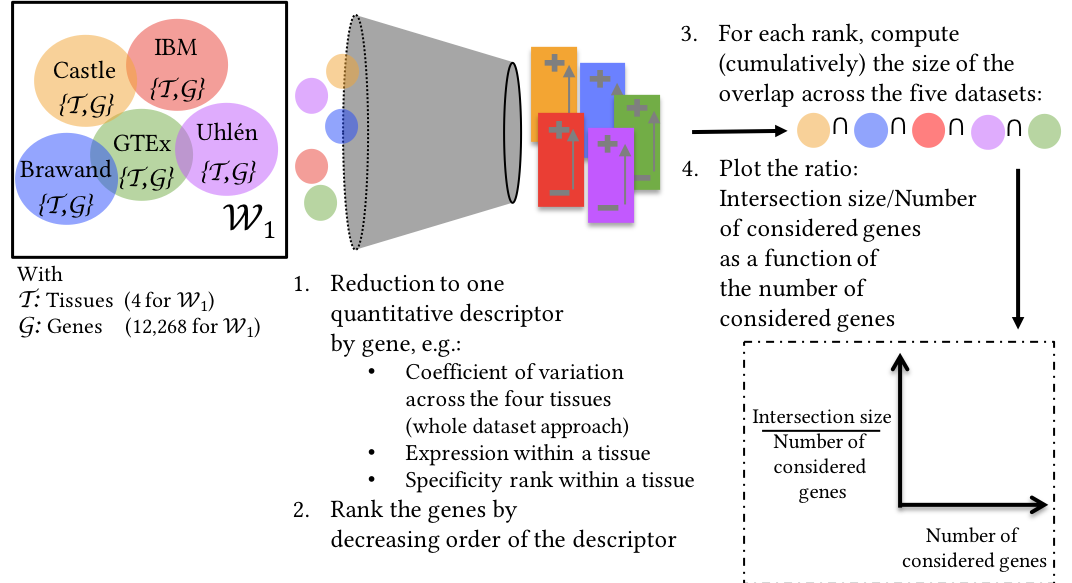
\includegraphics[scale=0.9]{transcriptomics/ConceptOverlap.png}\centering
    \caption[Overview for the comparison of the genes across the five
    studies based on a ranked descriptor 5 studies]{\label{fig:overlapConcept}%
    \textbf{Overview for the comparison of the genes across the five
    studies based on a ranked descriptor.}
    The first step applies individually to each of the studies
    within the working dataset (\ie\ here \setOne).
    It consists in extracting a single value per gene
    (\eg\ a statistic or any other quantitative descriptor)
    either for the entire \emph{d}ataset (referred thereafter as \emph{D-approach}) or
    for each \emph{t}issue in each dataset (referred as \emph{T-approach}).
    The next steps include
    computing (cumulatively) the intersection size number for each rank
    and plotting this number divided by the rank
    in function of the number of considered genes (\ie\ rank).}
\end{figure}

\Cref{fig:cvEvol5DF} presents the result.
Many of the most variable genes are commonly present in the top tier of the
five studies, though they have different individual rank.
Indeed, there is a strong growth for about the first 1,250 genes that then
settles a plateau which increases toward the final ratio ($1$).
Using the first quarter of the most variables genes as a cut-off appears
to be an acceptable threshold
as it comprises the primal growth and part of the plateau.

\begin{figure}[!ht]
    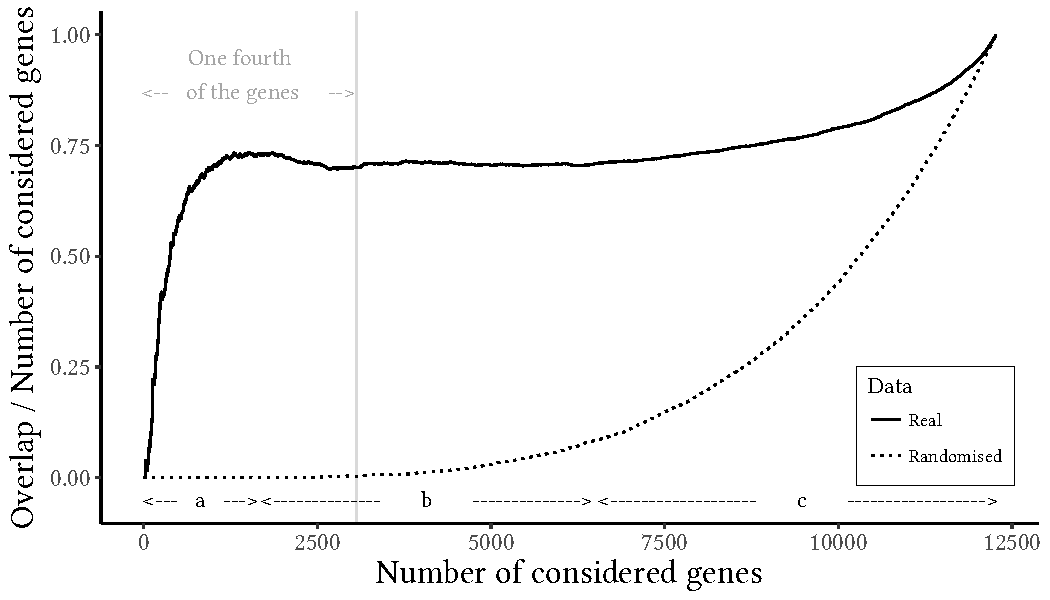
\includegraphics[scale=0.9]{transcriptomics/CVevolCumul5DF_line-abc.pdf}\centering
    \caption[Intersection size of \setOne\ genes (ranked by cv)]%
    {\label{fig:cvEvol5DF}\textbf{Intersection size course
    of \setOne\ genes (based on their coefficient of variation rank
    in each of the five studies).}
    There are three main parts.
    There is an initial strong growth (a)
    %followed by a short plateau (b)
    %before a slight decrease (c)
    which then settles a plateau (b).
    Eventually, the ratio increases slowly again
    until reaching the expected ratio of $1$ once all the genes from \setOne\
    are included (c).
    The first quarter of the genes covers (a) and a part of (b).
    Apart from (a),
    the overlap of shared genes between the five datasets when ranked on their
    coefficient of variation is above 70\%.
    The sigmoid curve (dashed line) is based on randomised data
    where permutations break the original order of the genes. (All the gene
    expressions levels within each dataset are permuted while the pattern of
    expression across the tissues is conserved. This operation is performed 10,000 times.
    The dashed line is a summary of all these permutations).
    There is a significant dissimilarity between the real and the randomised data.}
\end{figure}

\begin{figure}[!ht]
    \captionsetup{singlelinecheck=off}
    \includegraphics[scale=0.75]{transcriptomics/CVevolCumul2DF_line-abc.pdf}\centering
    \caption[Intersection size of \setTwo\ genes (ranked by cv)]%
    {\label{fig:cvEvol2DF}\textbf{Intersection size course
    of \setTwo\ genes (based on their coefficient of variation rank
    in each of the two studies).}
    Globally, there are two parts: one initial strong growth (a) and
    a second part (b) where the curve shifts shallowly towards
    the expected final ratio of 1.
    While the number of genes involved in \setTwo\ is higher than in \setOne,
    the ratio of common genes that are the twentieth most variable in each study
    is above 75\%.
    There are three main reasons that may explain this improved result compared
    to \Cref{fig:cvEvol5DF}.
    {\small
    \begin{itemize}[topsep=0pt,nosep,leftmargin=95pt,listparindent=5pt]
       \item \setTwo\ involves a smaller degree (\ie\ number of studies)
           than \setOne\ (respectively 2 and 5).
           Hence, bigger intersection sizes are easier to occur.
       \item As previously mentioned, \gtex\ and \uhlen\ studies provide probably
           more accurate \treps\ than the other studies (see~\vref{seg:betterTreps}).
       \item The greater number of tissues induces a wider range of \cvs,
           which allows picking up genes with more subtle variations.
   \end{itemize}}
    }
\end{figure}

\begin{comment}
If the previous analysis was to include
only the first 1,250 most variable genes
the results of \Cref{fig:heatmapMost25pVariable} may be even greater.
However, the dissimilarities highlighted by \Cref{fig:ReverseheatmapMost25pVariable}
would also be greater.
\end{comment}

In conclusion, while the most variable genes have a significant influence
on the strong and biologically meaningful correlations,
there must be other gene categories contributing.

One main drawback when considering the most variable genes is
the descriptor summarises the genes across all the tissues.
So,
the results may significantly vary
depending on the composition of the working set,
and this analysis may need to be rerun.

\subsection{Genes with tissue-specific (TS) expression}\label{sub:TisSpeGene}

Another good candidate to drive higher correlations
between identical tissue interstudy \treps\ than intrastudy different ones
are the genes that have an expression profile
that varies according to the tissues.
As reported before,
most \mRNAs\ are expressed in every tissue~\mycite{ramskoldan:2009}
(see also~\cite{Uhlen2015,GTExTranscript} for other examples) and
their expression is relatively invariant across the tissues (\Cref{fig:HistCV4T}).
Moreover,
many of the most variable genes
have a regular gene expression across the different tissues
aside one or two where the expression is notably higher globally
(see \Cref{fig:expressionMostvariableG}).
Thus,
considering genes with a \gls{TS} expression
seems a reasonable approach to explain the high correlations.

The definition of tissue specificity is unclear and
varies from one study to another (see also~\cite{Santos2015-rj}).
\cite{Liang2006-mk} define \emph{tissue specificity}
only for genes expressed solely in one tissue,
and then \emph{tissue selectivity} for genes expressed in more than one tissue
with an expression enriched in one or a subset of tissues.
Other studies have a broader definition of tissue specificity.
They identify genes above a given threshold of tissue selectivity (or enrichment)
as tissue-specific genes.
See for examples~\cite{Uhlen2014,Jiang2016-sv}.
In this second case,
genes with a single-tissue expression are an extreme case of \gls{TS} genes.

Within this thesis, I use the second definition,
\ie\ I consider genes as \gls{TS}
as long as they display a higher tissue selectivity than a preset threshold,
regardless how many tissues express them.
Indeed, every study present a subset of genes
that are expressed above 1\FPKM\
in a sole tissue (see \Cref{fig:breadthGenesP1}).
However, the decreasing number of these genes
when increasing the number of considered tissues highlights
the arbitrary relativity introduced by the study design.

Even for the second definition only,
there are many methods to characterise genes tissue-specificity in the literature.
See~\cite{Cavalli2011-bo,Xiao2010-mz,Karthik2016-mu,Kim2017-dz,Kryuchkova-Mostacci2017-mk,Kadota2006-eb,Yu2006-ha,Martinez2008-bm}
for some examples.
There are also databases that record previously identified \gls{TS} genes,
for normal conditions,
\eg\ \WebFoCi{TiGER}{http://bioinfo.wilmer.jhu.edu/tiger/}{tiger} or
\WebFoCi{TiSGeD}{http://bioinf.xmu.edu.cn:8080/databases/TiSGeD/index.html}{Xiao2010-mz}
and more specialised ones, \eg\ for cancer
\WebFoCi{TissGDB}{https://bioinfo.uth.edu/TissGDB/index.html}{Kim2017-dz}.

Amongst all the possible approaches to characterise the \gls{TS} \pcgs,
I detail three that I used in the following subsections.
First, I have queried \gls{TIGER} to capitalise on previous knowledge.
Then, to derive the \gls{TS} genes directly from \setOne\ and \setTwo,
I have used a commonly accepted method described in the literature,
that uses the gene expression \emph{fold change} ratio across the tissues.
Finally, I have diverted a robust method to detect outliers,
\ie\ the Hampel's test \mycite{Hampel1974},
to identify genes which present an unusual expression level in a single tissue.
In fact, as gene tissue selectivity and tissue specificity definitions are
relative to a context,
if the later changes,
the genes attributes may change as well
(\eg\ one gene that is unspecific in \setTwo\ may be \heart{}-specific in \setOne).


\subsubsection{Use of prior knowledge: TiGER database}\label{subsub:Tiger}

\gls{TIGER}~\mycite{tiger} reports \gls{TS} genes for thirty independent tissues
(based on \glspl{EST} experiments).

After retrieving the list of genes for all reported tissues,
I have mapped the \gls{Refseq} identifiers provided by \gls{TIGER}
to \gls{Ensembl} gene identifiers (\hg{38}, \ens{76}).
Then, I removed all duplicates due to the identifier translation within each tissue,
and I also filtered out all the genes identifiers that
I found in more than one tissue:
\gls{TIGER} lists a subset of the same genes in many tissues,
but the modification in the annotation may also explain part of the
repetitive genes.
Thus, for each tissue,
I have a list of identifiers that are specific to that tissue only.

\begin{figure}[!ht]
    \includegraphics[scale=0.85]{transcriptomics/Tiger5DF4Tissues.pdf}\centering
    \caption[Expression heatmap of the four tissues across the five datasets based on
    TiGER]{\label{fig:TigerGenes}\textbf{Expression heatmap of the four tissues
    across the five datasets based on \gls{TIGER} information.}
    This heatmap illustrates three subsets of genes:
    genes for which real expression data confirm their \gls{TIGER} definition;
    genes lacking to show any \gls{TS} profile in their expression data; and
    genes with mismatching tissue specificity between \gls{TIGER}
    definition and the expression data.
    The colorbar above the heatmap is representing the tissue
    for which \gls{TIGER} annotates the genes (presented as columns) as \gls{TS}
    (red for \Heart, green for \kidney, light orange for \liver\ and blue for \testis).
    %{\small
    %    \begin{itemize}[topsep=0pt,nosep,leftmargin=15pt,listparindent=5pt]
    %    \item Genes for which real expression data confirm
    %        their \gls{TIGER} definition.
    %    \item Genes lacking to show \gls{TS} profile in the expression data.
    %    \item Genes with mismatching tissue specificity between \gls{TIGER}
    %        definition and the expression data.
    %\end{itemize}
    %}
    \gls{TIGER} definitions may be quite accurate or not
    %(at least for \Rnaseq\ expression data).
    A substantial set of genes with available \gls{TIGER} definition is missing
    from the heatmap as their expression profile is overly similar across
    tissues and studies.
    Besides, I had to filter out genes with \gls{TIGER} duplicated definitions
    in independent tissues.
    Hence, it is challenging
    to predict which definitions are accurate \latin{a priori}.
    }
\end{figure}

\Cref{fig:TigerGenes} is an expression heatmap based on
a (partial) subset of \pcgs\
that are present in this final list of translated \gls{TIGER} genes.
There are three main types of genes.
The largest group comprises the genes with a corroborating profile
between the \gls{TIGER} definition and the real data.
Then, a second smaller group encompasses genes
listed as \gls{TS} in \gls{TIGER},
but lack to demonstrate expression specificity
towards any tissue in the real data.
Finally, the third group includes a very tiny subset of genes which
are more specific to another tissue than the initially stated one.

Without any additional knowledge,
it is difficult to predict which \gls{TIGER}
definitions will be confirmed (or not) by expression data.
Remarkably, most of the genes present the same trends
through the tissues within each of the studies regardless of their category.
Once again, \castle\ expression data is exhibiting
the only few observed discrepancies\footnote{Reminder:
the \gls{FPKM} quantification (used here) is sensitive
to the number of identified genes (see \Cref{eq:rpkm-fx}~\vref{eq:rpkm-fx})
and \castle\ study identifies and quantifies many more \glspl{RNA} than the
other studies as it uses a whole \RNA\ protocol
while the others are using polyA-enrichment (see \Cref{ch:datasets}).}.

\subsubsection{Fold change method}\label{subsub:TisSpeGeneMethodPerso}

As~\cite{DESeq2} noted the most common approach to detecting
a gene expression difference between two conditions is
to study the expression fold change (FC) ratio between these conditions.
This approach is inappropriate for direct use
with differential study\footnote{I.e.\ treated (diseased)
versus control samples comparison study.}
designs for many reasons and
needs corrections~\mycite{Anders2010-vq,DESeq2,Soneson2013-pd,edgeR}.
However, this method is still broadly present in the literature,
especially for studies other than differential gene expression analyses.
As examples, see~\cite{Uhlen2015,Zhu2016-xo,Yu2015-uh}.
Besides, \egxa\ \mycite{EBIgxa} relies on this method to select the genes
it displays as the most specific for \emph{baseline} studies\footnote{In
contrast with differential gene studies,
the baseline studies focus on
depicting the expression landscape of each covered condition
instead of focusing on the gene expression through these conditions.}.

There are also a few variations
on how to compute this ratio (see~\cite{Zhu2016-xo,Uhlen2015}).
In this thesis,
I compute the FC ratio by dividing the expression
of each gene in a given tissue
by the maximum expression of this gene across all the other tissues of that study
in the working set.
Studies usually pick arbitrary cut-offs to characterise the specific genes.
\cite{Uhlen2015} uses $2$ and $5$ cut-offs
to determine \emph{enriched} and \emph{enhanced} tissue genes.
\cite{Zhu2016-xo} set their cut-off at $2$ to characterise \gls{TS} protein-coding
and noncoding transcripts.
However,
I avoid arbitrary cut-offs, and
I use the FC ratio to rank the \pcgs\ of my working datasets according
to their specificity within each tissue:
higher FC ratios indicate genes with higher specificity.
I then assess the consistency of the tissue specificity of the genes through the
various studies.
For that, I have followed the \emph{T-approach} overviewed in \Cref{fig:overlapConcept}.

\begin{figure}[!ht]
    \includegraphics[scale=0.8]{transcriptomics/mostSpe4TP1.pdf}\centering
    \caption[Intersection size curve of \setOne\ genes based on their FC ratio
    rank in each tissue across the five studies]{\label{fig:mostSpe4T}\textbf{Intersection
    size curve of \setOne\ genes based on their specificity (FC ratio rank)
    in each tissue across the five studies.}
    One-fortieth of \setOne\ \pcgs,
    when ranked by specificity in \heart, \kidney\ and \liver,
    are commonly shared between the five studies.
    For \testis, the shared amount of genes reaches more than one-tenth of \setOne\
    whole set of genes.
    Compared to the most variable genes (\Cref{fig:cvEvol5DF}:
    \nameref{fig:cvEvol5DF}),
    the most specific genes seem to be more consistent across the studies.
    }
\end{figure}

\Cref{fig:mostSpe4T} presents the shifts in the intersection size curves of the
four tissues of \setOne.
The most specific genes in each tissue of \setOne\ are shared between the
five studies.
Indeed, the slopes are very sharp before reaching a peak and dropping as sharply
for the first fortieth genes in \heart, \kidney\ and \liver.
The intersection of the most specific genes is even greater for \testis\ as
it concerns more than a tenth of \setOne\ genes.

\begin{figure}[!ht]
    \includegraphics[scale=0.75]{transcriptomics/mostSpe23TP1.pdf}\centering
    \caption[Intersection size curve of \setTwo\ genes based on their FC ratio
    rank in each tissue across the two studies]{\label{fig:mostSpe23T}\textbf{Intersection
    size curve of \setTwo\ genes based on their specificity (FC ratio rank)
    in each of the twenty-three tissues across the two studies.}
    }
\end{figure}

Thus, the \gls{TS} genes are also contributing to provide a stronger
biological signal over the technological noise.

\subsubsection{Hampel's test: detection of \emph{untypical} expression}\label{subsub:Hampel}

Much interlaboratory or interstudy research in the literature use the Hampel's test,
\eg~\cite{LinsingerHampel,Lewczuk2006-wq,Rocke1983-qa,Apfalter1999-ca}.
In fact, the Hampel's test is a robust method
for detecting outliers~\mycite{Davies1993-nv,Pearson2002-im}
in data that are identically and independently distributed (i.i.d.)~\mycite{Liu2004-kf},
while easy to implement and use~\mycite{LinsingerHampel}.
This method uses the median, the \gls{MAD} and a cut-off to define the outliers.

For this thesis, I have derived this test to identify conditions (\ie\ tissues)
where the gene expression is \emph{untypical}.
I rely on the two facts that
most genes are expressed everywhere \mycite{ramskoldan:2009,Uhlen2015,GTExTranscript}
(see also \Cref{fig:breadthGenesP1}),
and they mostly present a limited variation in their expression
through the various tissues (see \Cref{fig:HistCV4T,fig:HistCV23T}).
Thus, when the expression of the gene is untypical
(\ie\ an outlier to the average profile of that gene expression across the many tissues),
it denotes a tissue specificity.
Besides,
this test allows detecting genes that are over- or under-expressed in specific tissues.
(Whereas the other methods are only detecting the overexpressed genes.)

After implementing the method (see \cref{algo:hampel})
with a (widespread) cut-off of $5.2$, % (which assumes a normal-like distribution),
I have applied it to the whole original datasets and \setTwo.
\setOne\ comprises too few tissues to allow detecting \emph{untypical} expression.
Overall, there are always more than 60\% of congruence between the genes tagged
as untypical in a specific tissue for the whole dataset
and the subset of twenty-three tissue.
The proportion of agreement between the partial and whole datasets increases,
even more, when I filter the results to keep only the genes that are recurrently
picked for both \uhlen\ and \gtex\ data.
Thus, though known as a robust method,
the Hampel test outcomes are still dependent on the set of considered tissues.

\begin{figure}[!ht]
    \includegraphics[scale=1]{transcriptomics/hampel5DF4Tissues.pdf}\centering
    \caption[Expression of the genes picked with Hampel method]{\label{fig:hampelExp}%
    \textbf{Expression of the genes picked consistently with the Hampel method
    in each study solely in one tissue.}}
\end{figure}

\Cref{fig:hampelExp} regroups the genes that the Hampel test detects
as outliers for the five studies for their four shared tissues.
All corresponding-tissue \treps\ present similar patterns of expression
regardless of their original study,
although the \castle\ \treps\ have overly lower expression than the others.
Other filters may improve the results:
\eg\ selecting genes with higher expression or
increasing the cut-off above $5.2$ in selected tissues.

\subsection{Uhlén categories}\label{sub:UhlenGeneCat}

Put together the results from the previous sections seem to describe that
the strong correlations are driven by different categories of genes.

Uhlén laboratory papers \mycite{Uhlen2014,Uhlen2015,Uhlen:2016},
use different categories of genes to describe the normal human transcriptome.
As their classification changes between these related papers,
I have redefined a classification based on them
(presented in \Cref{tab:UhlenCat})
before applying it to \setOne\ and \setTwo\ (\Cref{tab:UhlenCategoriesProtCoding}).

\begin{table}[!htpb]
\centering
\caption[Gene classification]{\textbf{Gene classification}\label{tab:UhlenCat}\\
\footnotesize{adaptation of \uhlen\ \etal\ classification~\mycite{Uhlen2014,Uhlen2015,Uhlen:2016}}}
\begin{tabular}{@{}ll@{}}
\toprule
Category        & Definition                                                                                           \\ \midrule
Not detected    & Never detected above 0 FPKM                                                                    \\
Not expressed   & Never detected above 1 FPKM                                                                    \\
Mixed high      & Expressed in a subset of tissues and always $\geq 10$ FPKMs                                     \\
Mixed Low       & Expressed in a subset of tissues and always $< 10$ FPKMs                                 \\
Ubiquitous High & Expressed in all the tissues and always $\geq$ 10 FPKMs                                         \\
Ubiquitous Low  & Expressed in all the tissues and always $< 10$ FPKMs                                     \\
Group enhanced  & Expressed in a subset of tissues with an expression $\geq 5*mean_{all~the~tissues}$             \\
Tissue enhanced & Expressed in a single tissue with an expression $\geq 5*mean_{all~the~tissues}$                 \\
Tissue enriched & Expressed in a single tissue with an expression $\geq 5*Max_{all~the~other~tissues}$ \\ \bottomrule
\end{tabular}
\end{table}

\Cref{tab:UhlenCategoriesProtCoding} shows that for many of these categories,
the number of shared \pcgs\ is high between the different studies of the
two working datasets.

\pagestyle{plain}
\begin{landscape}
\begin{table}[]
\centering
\caption[Uhlén et al.\ gene categories]{\label{tab:UhlenCategoriesProtCoding}%
\textbf{Uhlén et al.\ gene categories}\\
\footnotesize{Apart the undetected genes and the ones expressed below 1 \FPKM,
a gene may be referenced in several categories.}}

%\begin{tabular}{@{}lllllllllll@{}}
\begin{tabular}{@{}ccccccccccc@{}}
\toprule
\multicolumn{2}{c}{\multirow{2}{*}{\begin{tabular}[c]{@{}c@{}}\ens{76}
    \\($\sim$22,500 protein\\coding genes) \end{tabular}}} &
\multirow{2}{*}{\begin{tabular}[c]{@{}c@{}}\\Not\\detected\end{tabular}} &
\multirow{3}{*}{\begin{tabular}[c]{@{}c@{}}Not expressed\\ at 1 \gls{FPKM}\\
    cut-off\end{tabular}} &
\multicolumn{2}{c}{Mixed expression} &
\multicolumn{2}{c}{Ubiquitous expression} &
\multirow{2}{*}{\begin{tabular}[c]{@{}c@{}}\\Group \\Enhanced\end{tabular}} &
    \multirow{2}{*}{\begin{tabular}[c]{@{}c@{}}\\Tissue\\ Enhanced\end{tabular}} &
        \multirow{2}{*}{\begin{tabular}[c]{@{}c@{}}\\Tissue\\ Enriched\end{tabular}} \\
    \cmidrule(lr){5-8}
\multicolumn{2}{c}{}
    &  &  &
    \begin{tabular}[c]{@{}c@{}}Low\\ (\textless\ 10 \gls{FPKM})\end{tabular} &
        \begin{tabular}[c]{@{}c@{}}High\\ (≥ 10 \gls{FPKM})\end{tabular} &
            \begin{tabular}[c]{@{}c@{}}Low\\ (\textless\ 10 \gls{FPKM})\end{tabular} &
    \begin{tabular}[c]{@{}c@{}}High\\ (≥ 10 FPKM)\end{tabular} &  &  &  \\
        \midrule
        \multicolumn{1}{c}{%
        \multirow{6}{*}{\rotatebox[origin=c]{90}{\parbox[c]{3cm}{\centering Whole
        dataset}}}} &
        Castle & 3,403 & 3,268 & 8,773 & 1,033  &
        1,399  & 634   & 11   & 3,664   & 1,975 \\
        \multicolumn{1}{c}{} & Brawand & 2,964 & 3,095 &
        8,034 & 1,788  & 1,760 & 958   & 0  &
        2,729  & 2,548 \\
        \multicolumn{1}{c}{} & IBM & 2,693 & 2,605  &
        7,325  & 1,406  & 1,135 & 858  & 322 &
        5,248  & 2,453  \\
        \multicolumn{1}{c}{} & Uhlén & 2,662 & 1,747 &
        5,769 & 1,053  & 456 & 406  & 2,511  &
        5,201  & 2,333  \\
        \multicolumn{1}{c}{} & GTEx & 2,197  & 1,886  &
        5,556  & 1,117 & 687  & 698  & 3,859  &
        4,356  & 1,919 \\ \cmidrule(l){2-11}
        \multicolumn{1}{c}{} & Consensus & 2,197 & 486  &
        1,749  & 221  & 33  & 161  & 0  & 677  &
        \begin{tabular}[c]{@{}c@{}}531 $[$518$]$\end{tabular} \\
            %\multicolumn{1}{c}{} & \footnotesize{without Gtex} &
            %\footnotesize{2,413} & \footnotesize{638} & \footnotesize{2,152} &
            %\footnotesize{286} & \footnotesize{63}  & \footnotesize{179} &
            %\footnotesize{0}  & \footnotesize{814} &  \footnotesize{587}  \\
            \midrule
\multirow{6}{*}{\rotatebox[origin=c]{90}{\parbox[c]{3.5cm}{\centering Common\\
4 tissues\\ Working datasets}}} &
Castle & 19,066 & 2,994 & 8,589 & 1,513 &
2,994 & 1094 & --- & --- & 2,185 \\
& Brawand & 19,505  & 2,962  & 8,626  & 2,228
& 2,962  & 1251 & --- & --- & 3,672  \\
& IBM & 19,776  & 2,989 & 8,534 & 1,954 &
2,989  & 1212  & --- & --- & 2,824  \\
& Uhlén & 19,807 & 2,917 & 8,367 & 2,227 &
2,917  & 1190  & --- & --- & 3,730  \\
& GTEx & 20,272 & 3,870 & 8,988  & 2,312 &
3,870  & 1427  & --- & --- & 3,554  \\
\cmidrule(l){2-11}
& Consensus & 1,973 & 550 & 3,351 & 649 &
550  & 439 & --- & --- & 1,412  \\
%& \footnotesize{without Gtex} & \footnotesize{2,413}  & \footnotesize{2,186}  &
%\footnotesize{3538}  & \footnotesize{639}  & \footnotesize{576}  &
%\footnotesize{439}  & \footnotesize{---} & \footnotesize{---} & \footnotesize{1,462}
\midrule
\multirow{3}{*}{\rotatebox[origin=c]{90}{\parbox[c]{1.7cm}{\centering Common\\ 23
tissues\\ Working datasets}}} & Uhlén & 2,662  & 1,970  &
6,160 & 1,135 & 594  & 427 & 1,285 &
5,776 & 2,518 \\
& GTEx & 2,197 & 2,258 & 6,966  & 1,540 &
1,822  & 997 & 1,048 & 5,496  & 2,460 \\
\cmidrule(l){2-11}
& Consensus & 2,197 & 1,544 & 4,936 & 791 &
423 & 417 & 558 & 4,223 & 1,885 \\
\bottomrule
\end{tabular}
\end{table}
\end{landscape}
\pagestyle{scrheadings}


\subsection{Curated sets}\label{subsec:Trans_curatedSets}
\Pcgs\ that were characterised consistently
as any of the aforementioned categories across the five datasets of \setOne\
or the two of \setTwo\
are provided as supplementary data.


\section{Discussion}\label{sec:Trans_discussion}

In this chapter,
I have directly combined and compared
the most extensive number to date of~\Rnaseq\ transcriptome
of normal human tissues together.
From them,
I have constructed two working datasets of \pcgs.
The first one (\setOne) comprises four tissues
and 12,268 shared genes
extracted from five independent studies
(\cite{Krupp2012,VTpaper,Uhlen2015,GTExTranscript} and \ibm)
and the second one (\setTwo) comprises twenty-three tissues
and 17,554 shared genes
from two studies (\cite{Uhlen2015,GTExTranscript}).
Clustering analyses (and \Welchttest) of these two sets
confirm that \Rnaseq\ technical noise is
lower that relevant biological signals present in the data.
Indeed,~\cite{Sudmant2015-zt,Danielsson2015-cn,Yu2015-uh} and~\cite{Uhlen:2016}
also observe that interstudy corresponding tissues pairs are more related than
intrastudy non-corresponding tissue ones
(average correlation for corresponding tissue-pairs $r=0.75$, $\rho=0.88$;
average for non-corresponding tissue-pairs $r=0.20$, $\rho=0.75$).
In an attempt to inspect possible underlying forces for the close \treps\
similarities across the studies,
I have considered different attributes and groups of genes:
\emph{highest expressed}, \emph{most variable}, \emph{most specific}.
The top highest expressed genes show a very small (if any) impact on
the interstudy tissue expression profile strong correlations.
The most variables and most specific genes have a real contribution even though
their importance may be relative compared to the whole set of expressed genes.
As the definition of \gls{TS} genes is very variable from one study to another
(see \cref{sub:TisSpeGene}),
I have relaid on three methods to pick them.
For one of the method,
I have extracted from an existent resources
\WebCi{TiGER}{http://bioinfo.wilmer.jhu.edu/tiger/}{tiger},
the list of \gls{TS} genes that I have then update to the more recent annotation
I use within my thesis.
Mining the experimental data with this updated list highlights
the need of cautiousness when dealing with older resources.
While the congruence of the three methods is partial,
the \gls{TS} genes show distinct expression profiles across tissues
that are rather consistent through the different studies.
Finally, through a classification inspired
by Uhlén et al.\ \mycite{Uhlen2014,Uhlen2015,Uhlen:2016}
and which considers together the breadth, the level and the specificity of expression,
I have explored the congruence of the genes categories across the studies.

Concomitantly, other research groups have published similar studies
since I started this project.
However, at the time of writing this thesis,
all the other studies (including the aforementioned ones)
were still based on the human genome built \hg{37} (or hg19),
while I am using the more recent \hg{38} one.
Moreover, these studies either have different focus, aims,
approaches or more limited scopes.
Thus, my work expands or completes theirs on different points.
\begin{itemize}[topsep=0pt,nosep]
%Feb 2016 -Uhlén
\item\fullcite{Uhlen:2016} In this review paper,
the authors present the results of~\cite{Yu2015-uh} and~\cite{Danielsson2015-cn}
that I discuss there below.
They also compare the \gtex\ released data~\mycite{Bahcall2015-mh,GTEx_Consortium2015-si,Gibson2015-wh}
to their own~(\uhlen\ data~\mycite{Uhlen2014,Uhlen2015}).
As they rely on other studies to confirm many findings,
their comparison of these two studies is
limited to the examination of
the proportion of genes in each category of their simplified classification
for (only) nineteen tissues.
We reach the same conclusions:
overall, there are significant overlaps across the datasets for each of the
categories (\enquote{Expressed in all}, \enquote{Not detected},
\enquote{Tissue enriched}, \enquote{Group enriched}, \enquote{Enhanced} and
\enquote{Mixed}).
%December2015 -Burge
\item\fullcite{Sudmant2015-zt}
The authors focus on interspecies, intertissue and interstudy comparisons.
The major issue of the study is its use of \gls{TMM} as gene expression unit.
\gls{TMM} normalisation has the assumption that
genes have a stable expression across the conditions.
They, however, limit their scope to very specific orthologs
since they explore \Rnaseq\ expression data across species, tissues and studies.
They also confirm that with \Rnaseq\ expression profiling,
the interstudy technical variation is generally lower than
the intrastudy biological one, \ie\
interstudy homologous tissues of the same species are usually
closer in similarity than intrastudy different tissues of the same species
(or matched tissues of different species).
They found that interstudy comparisons are more variable for \species{human}
than other species.
They finally note that this kind of meta-analysis is dependent on
the choice of tissues to be studied.
%June2015 - Yu
\item\fullcite{Yu2015-uh} integrate \uhlen\ \etal\ data~\mycite{Uhlen2014}
with \gls{CAGE} peak expression data from the \gls{FANTOM5}
consortium~\mycite{FANTOM5-cage}.
Overall, their analyses are very similar to the ones I have presented in this
chapter.
In fact, we reach similar conclusions as well:
\begin{itemize}[nosep,topsep=0pt]
\item Overall gene expression is comparable through their two datasets.
\item Tissue expression signatures are independent of the data set (and profiling method).
\item Global comparison of ubiquitously expressed and \gls{TS} genes are comparable
    across the two studies
\item They compare the two datasets at gene levels because of the lack of accuracy
    of the current \Rnaseq\ protocols and algorithms and focus on the \pcgs\
    as the level of agreement between the two studies is low
    (which they attribute to the polyA-selected protocol of \uhlen\ \etal\ data).
\end{itemize}
Besides the choice of the original studies,
the few differences are (1) the version of the annotation
(they use the previous human genome built (\hg{37})) and
(2) their more simplified classification for ubiquitous and \gls{TS} genes.
They are also more lenient to assess the congruence (\eg\ expressed in all tissues
in one dataset and 95\% of the tissues in the other datasets is considered as
concordant).
Strikingly, they also find a discrepancy with \salivary\ compared to the other tissues
as I have noticed myself\footnote{\salivary\
is the only tissue for which \uhlen\ and \gtex\ show a Pearson correlation coefficient
$r<0.65$.}
%March2015
\item\fullcite{Danielsson2015-cn} cover three different tissues
(\brain{}\footnote{Either \cortex\ or \hypothalamus}, \heart, \kidney)
extracted from five projects (\cite{Burge,VTpaper,Uhlen2015,Krupp2012} and \ibm).
Their study is limited to
the comparison of precomputed to uniformly reprocessed data.
They are exploring experimental factors of variation and possible correction strategies.
They reveal that original precomputed data have considerable study-specific biases.
Their results on interstudy tissue similarities are superficial.
One of their most \enquote{fine-grained} results is the very low number of shared
genes amongst the hundred most expressed genes
for the three tissues across their five datasets.
%June2015 - SciRep-Zhu
%\item\fullcite{Zhu2016-xo}
%June2015 -Santos
\item\fullcite{Santos2015-rj} focus on the congruence of gene---tissue association
through different types of expression data (transcriptome and proteome)
and resources.
They report that most genes are either expressed in every
considered tissue or in small subsets in their constructed working dataset.
They also find that tissue specificity global trends are similar,
even if there are many discrepancies of gene presence for a same tissue
across the original datasets.
They have integrated together five tissues
(\heart, \kidney, \liver, \nervous\ and \intestine)
from five transcriptome datasets that they use \enquote{as-is}\footnote{%
In fact, even for their follow-up paper \mycite{Palasca2018-fh}
where they reprocess all the \Rnaseq\ data
for \species{mouse}, \species{rat}, \species{pig},
they do not mention any improvement made on the \species{human} \Rnaseq\
data (either in the results or methods and data).},
before refining a complementary set that comprises only the three highest-quality
datasets: \WebFoCi{UniGene database}{https://www.ncbi.nlm.nih.gov/unigene}%
{Wheeler2003-dv,unigeneNcbi}, \uhlen\ \etal\ data (HPA \Rnaseq)~\mycite{Uhlen2014,Uhlen2015}
and \castle\ \etal\ (\Rnaseq\ atlas)~\mycite{Krupp2012} for which they provide
association data for 14,722 genes.
They forsake the exploration of gene expression by correlations
but examine the tissue association enrichment
through the gene expression fold change.
The main issue with their transcriptomic study is their
assumption that higher expression\footnote{\FPKM\ values are directly
used as score for true presence and selectivity to a tissue} means
more robust gene---tissue association
which may often be translated (but wrongly) to a greater tissue-specificity.
%Sep2017
\item\fullcite{Wang2017-hc} (unreviewed paper) have used
subsets of \gtex\ and \tcga\ raw data that they have quantified \mRNAs\ at
transcript levels with \hg{37} (hg19).
They have corrected for the study effect with \softCi{ComBat}{Johnson2007-xh}
and have released the normalised data to the community.\\
\NB\ \egxa\ provides more recent versions of the \gtex\ and \tcga\
(as a part of the \pcawg\ project) data.
%Sept.2014
\item\fullcite{seqcmaqc} have found that relative expression measurements
by \Rnaseq\ are accurate and reproducible across sites.
The authors also showed that the overlap of identified and characterised genes
is imperfect (~91\%)
even when the design includes
the same two well-characterised reference RNA samples across all sites.
Also,
this specific design prevents inferring how the biological signal
may compare to the individual variations and the possible noise introduced
by collection, storage and extraction protocols.
\item Several papers (\cite{Khang2015-qt,ruvseqComQN,Rau2014-va})
    explore the reliability of \Rnaseq\ in the context of
    \gls{DGEA} that I will not discuss.
\item\cite{Zhuo2016-qi} explore the stable expressed genes across multiple
    (24) \Rnaseq\ studies for \species{Arabidopsis}
    which is why I will not discuss it further.
\end{itemize}

Unsurprisingly,
updating the human genome version from \hg{37} to \hg{38}
for the reconstruction
step\footnote{See \Cref{subsec:reconstruction}: \nameref{subsec:reconstruction}}
enhances the results significantly.

Besides, as my analyses were incorporating more studies,
the results improved greatly
(in particular with the inclusion of \uhlen\ and \gtex\ studies).
Indeed, as I focalise my analyses on the common set of genes across the studies,
I remove the most interstudy variant genes, and
I bias the analyses towards the genes
for which \Rnaseq\ is more robust to quantify their expression profiles.
Hence, it may be interesting to relax the filters by including genes
that are found in any two or more datasets as a follow-up study.


\section{Conclusion}

While the expression levels are hard to translate directly from one study
to another~\mycite{Yu2015-uh,Santos2015-rj},
many facts have been confirmed in this thesis and the studies mentioned before:\begin{itemize}[nosep,topsep=0pt]
        \item Tissues are clustering preferably with corresponding
            (or closely biologically related) tissues even across studies
            rather than clustering with different tissues from the same study
            (\ie\ biological signal $>>>$ technical noise due to \Rnaseq\ protocols).
        \item More recent transcriptome studies are more congruent than previous ones.
        \item \testis\ presents the highest number of \gls{TS} \pcgs\
            (see \Cref{fig:UniqExprPC1}).
            It also presents the most variety of expressed \pcgs\ ($≥1$ \FPKM)
            \castle, \brawand, \ibm\ and \uhlen\ studies.
            (This extend to \gtex\ study if all detected genes (\ie\ above 0 \FPKM)
            are considered.)
        \item \liver\ has the most robust \gls{TS} \pcgs,
            which may be explained by greater knowledge
            and better annotation than the other tissues.
        \item Most genes are expressed everywhere (ubiquitous) and
          a smaller proportion of them are expressed in a very limited set of tissues.
        \item Well-differentiated tissues have specific expression profiles
            that allow using processed data \enquote{as-is} for rough comparisons
            such as sample swap checks
            or quality controls, \eg\ \salivary\ in \uhlen\ \etal\ data which
            presents low correlation with
            \gtex\ data (see \Crefp{fig:SamedistribPearsCorr}{}) and with
            FANTOM5 data~\mycite{Yu2015-uh}.
        \item Annotations have an essential effect on the final results.
              Thus, we ought to keep whenever possible the resources up-to-date.
\end{itemize}

In addition,
put together the results seem to indicate that
gene expression profiles are comparable from one study to another even though
it is challenging to describe them for particular given genes.
Also, single distinct gene attributes have a reduced effect on the correlations.
The equivalent gene expression tissue profiles across the studies
are probably due to additive effects from every (or almost) expressed gene.
This is rather concerning as many studies (\eg{}~\cite{Sudmant2015-zt})
use normalisation methods explicitly developed for \glsxtrfull{DGEA}
for other kinds of analyses (similar to this chapter analyses).


Thus, there is an evident need for more multi-tissue studies
with biological replicates to refine and complete these findings.
New strategies, notably normalisation methods, have to be also developed
to allow the easy reuse of uniformly processed and quantified data by
the community.
%\cite{Roca2017-zi} have developed a new normalisation method in an attempt
%to provide a potential alternative solution.
Ideally, the final aim should be to provide a general human transcriptome build
as it already exists for the genome.
Finally, as long as the annotations are redefined and refined,
it~also~means~that~periodic~resources~reprocessing~may~be~inevitable.


\chapter{Human MS-based Protein expression landscape}\label{ch:proteomics}

\setlength{\epigraphwidth}{0.7\textwidth}
    \setlength{\epigraphrule}{0pt}
    \epigraphhead[5]{%
    %\epigraph{\emph{On m'a enseigné que la voie du progrès
    %n'était ni rapide ni facile.}}{Marie Curie}
    \epigraph{\emph{I was taught that the way of progress is
    neither swift nor easy.}}{Marie Curie}
}

After exploring the high-throughput human transcriptomic studies
in \Cref{ch:Transcriptomics}
and before integrating them with proteomic data in \Cref{ch:Integration},
I present in this chapter the comparison of
the three proteomic datasets introduced in \Cref{ch:datasets}.
\citet{Ezkurdia2014-qx,Deutsch2015} have partially reviewed these data.
However, we have reprocessed them starting from the raw data
for this thesis.
In this context, reassessing the quantified processed proteomic data
before any integration is pertinent.

The work presented in this chapter was done in collaboration with \james\
who has implemented the new protein quantification method
(presented in \Cref{sec:NewQuantProt}).
I have received general feedback from \alvis, \mar,
\sarah\ and Faranak Ghahreman.
A manuscript describing part of this chapter's work
and the one presented in \Cref{ch:Integration} is being prepared.

\section{An~overall~fragmented~and~disparate~universe~to~explore}

As I have described in \Cref{ch:background},
proteins present a wide range of physicochemical properties
(see \Cref{sec:bio} and \Cref{sec:aa})
and are challenging to identify and quantify
in high-throughput studies (see \Cref{sec:exploreProtMS}).
Thus, it comes as no real surprise that
while the use of \ms\ for proteomics has been developing since the 1980s~\mycite{BiomolBio},
the first notable attempts to draft the human proteome occurred only recently
in 2014~\mycite{PandeyData,KusterData},
or that the oldest (unpublished) available multi-tissue \cutler\ dataset is from 2010
(see \Cref{subsec:cutler}).
To this date,
\cutler Lab, \kuster\ Lab and \pandey\ Lab datasets are the only ones
that explore concurrently several nondiseased human tissues.
See \Cref{sec:ProteoData} for more details and
the processing pipeline designed and implemented by \james\ to handle them.

As presented in \Cref{fig:VennDiagProt3},
they share four tissues: \heart, \lung, \ovary\ and \pancreas.
The protein overlap of this four-tissues set between these three datasets
is rather narrow as shown in \Cref{fig:VennProtComm}.
The \cutler\ Lab dataset is the most limiting factor;
\pandey\ Lab and \kuster\ Lab datasets share over twice as many proteins
that they share with \cutler\ (3,338 instead of 1,384).
The number of shared proteins between \pandey\ Lab and \kuster\ Lab data rise to 4,172
when all their fourteen common tissues are considered.

\begin{figure}[!htpb]
    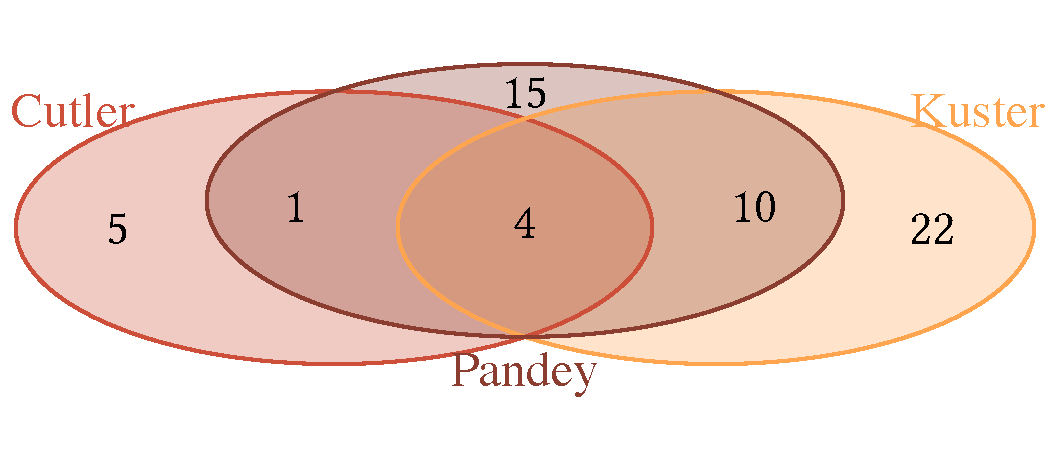
\includegraphics[scale=0.71]{proteomics/VennDiagProtCond.pdf}\centering
    \vspace{-5mm}
    \caption[Distribution of unique shared tissues between
    the 3 MS-based proteomic studies]{\label{fig:VennDiagProt3}\textbf{Distribution
    of unique and shared tissues between the three MS-based proteomic studies.}
    The three datasets share together: \heart, \lung, \ovary\ and \pancreas.
    The two most recent studies share fourteen tissues in total;
    the additional ten tissues are: \adrenal, \hcolon, \gallbladder,
    \oesophagus, \kidney, \liver, \placenta, \prostate, \rectum\ and \testis.}
\end{figure}
%\vspace{1cm}
\begin{figure}[!htpb]
    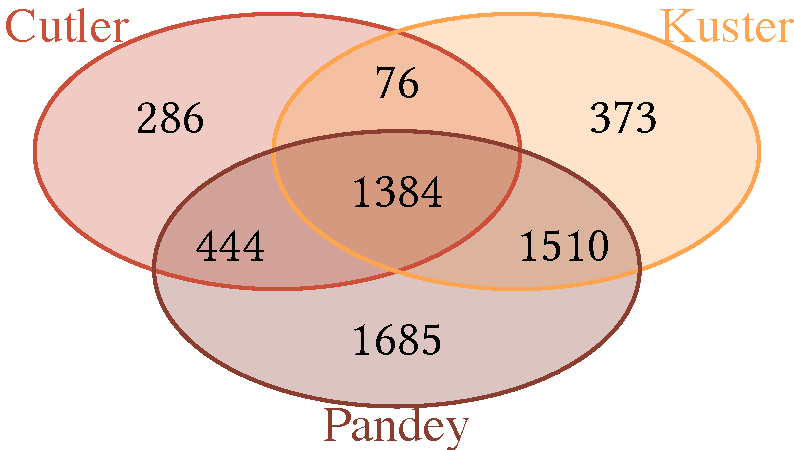
\includegraphics[scale=0.75]{proteomics/VennDiagProtFor4T.pdf}\centering
    \vspace{-5mm}
    \caption[Proteins overlap between the common tissues of
    the 3 proteomic studies]{\label{fig:VennProtComm}\textbf{Proteins
    overlap between the common four tissues of the three proteomic studies.}
    Unique and shared proteins detected and quantified
    across the three \ms\ studies for their four shared tissues:
    \heart, \lung, \ovary\ and \pancreas.}
\end{figure}
\clearpage
\subsection{High-throughput MS proteomic data has high detection variability}

\Cref{fig:barplot3Dvennprot}
illustrates the number of proteins identified in each of these four tissues.
The colours indicate in which dataset (or group of datasets)
the proteins have been identified.
See \Cref{fig:protbkdownT} for each set precise numbers.

\begin{figure}[!htbp]
    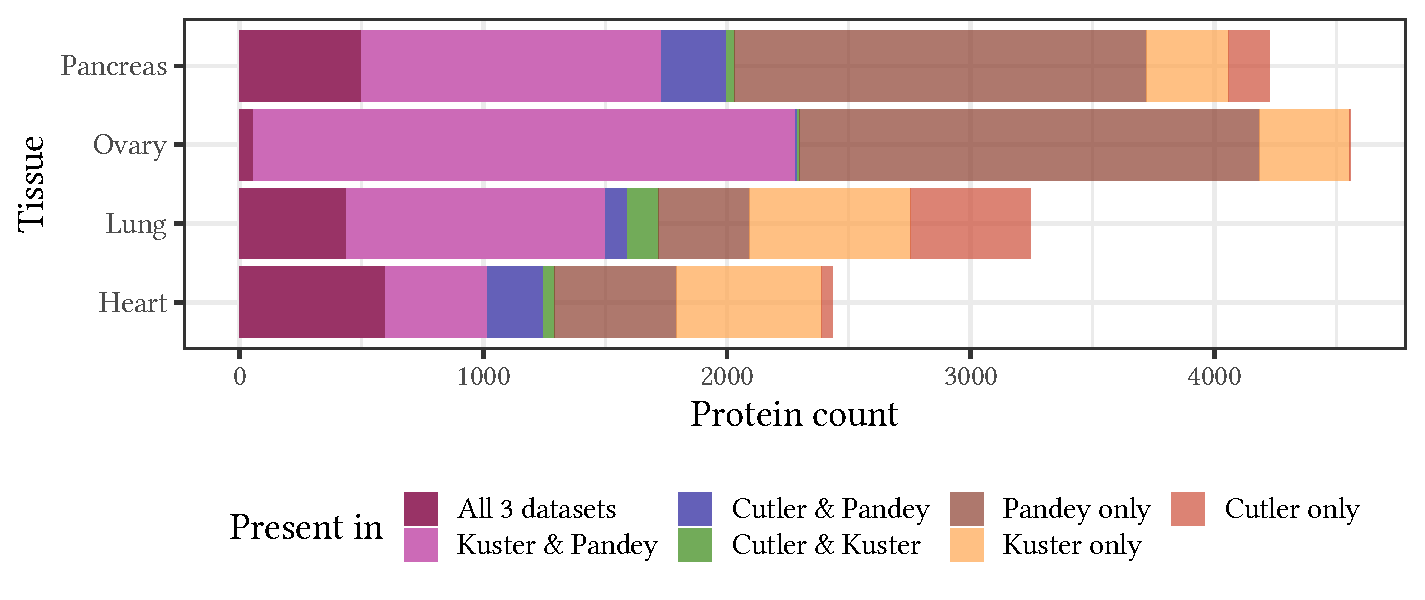
\includegraphics[scale=0.65]{proteomics/barplotVenn3Dprot.pdf}\centering
    \vspace{-3mm}
    \caption[Identified proteins across the 4 shared tissues for the 3 datasets]%
    {\label{fig:barplot3Dvennprot}\textbf{Number of identified
    proteins in each of the four common tissues for the three proteomic data.}
    Proteins found in more than one dataset are most likely true (in
    red, light and darker green or purple --- the most validated ones in red
    as they are found in all three datasets).
    See \Cref{fig:protbkdownT} for the precise numbers in each set.}
\end{figure}

The tissue with the highest number of identified proteins,
regardless of which dataset,
is the \ovary.

The highest number of proteins identified in all three datasets at once (600)
is in the \heart.
The other tissues have
the \emph{Kuster and Pandey} set as
their largest protein group formed by more than one dataset.

The largest set of identified proteins in \pancreas\
and the second one in \ovary\ are proteins only found in \pandey\ Lab dataset
(\emph{Pandey only}).
As shown in \Cref{fig:distribProtUniq3D},
our pipeline has identified the highest number of proteins in the \pandey\  Lab dataset.
Thus, it is coherent that \pandey\ Lab proteins represent a large part of
the identified proteins in each tissue (either as \emph{Pandey only} set or
in agreement with the other datasets:
\emph{All 3 datasets}, \emph{Kuster \& Pandey} or \emph{Cutler \& Pandey}).
More surprising is that the \cutler\ dataset comprises a respectable amount of
proteins in \lung\ that are missing in the other two.
A few of these proteins (82) are missing altogether,
but a subset of them (410) is still found
in (at least) another tissue of the other datasets.

\begin{figure}[!htpb]
    \includegraphics[scale=0.8]{proteomics/ProteinUniqueDistribPerdatasets.pdf}\centering
    \caption[Distribution of the proteins per tissue]{\label{fig:distribProtUniq3D}%
    \textbf{Distribution of the proteins per tissue across the three datasets.}
    \cutler\ Lab dataset has the smallest and \pandey\ Lab the highest number of proteins
    per tissue.
    Coloured in red are the proteins that have uniquely been identified
    in one tissue (or cell type) in each dataset;
    in turquoise are proteins that have been identified in several samples
    of the dataset.}
\end{figure}

While proteins found in more than one dataset are more likely true positives,
it is impossible to exclude without risks the ones
that are identified in one dataset only.
Whether an identified protein in one dataset is
an artefact (\ie\ false positive) or a miss (false negative) in the other datasets
is a challenging question;
the diversified nature of proteins involves
many sample preparation and simplification methods
(see \Cref{subsec:ProtSampPrep,subsec:simpleProt}).



%\vspace{-0.5cm}

\subsection{About half of the identified proteins are found in the same tissue
in different datasets}\label{subsec:halfProtConfirmed}

As shown in \Cref{fig:barplot3Dvennprot,fig:protbkdownT,fig:protbkdownT10more},
besides a few exceptions (\oesophagus, \gall\ and \testis),
more than half of the proteins are identified in the same tissue
in more than one dataset.
Three proteins are found in every tissue of every dataset:
\protein{ALB},  \protein{KRT9}, \protein{KRT10}.
This number rises to forty when only the \pandey\ Lab and the \kuster\ Lab data
are considered (see \Cref{tab:ubiProt2D}).
I have also investigated tissue-specific (\gls{TS}) proteins
(in red in \Cref{fig:distribProtUniq3D})
that are also identified in more than one dataset.
While the three datasets lacked to identify any \gls{TS} protein at once,
\pandey\ Lab and \kuster\ Lab datasets share a few (44 across eight tissues)
--- see \Cref{tab:comTSprot} for the complete list.
\begin{comment}
twelve for \kidney, nine for \placenta, seven for \pancreas,
five for \adrenal\ and \liver, four for \testis,
and one for \prostate\ and \rectum.
\end{comment}

\gls{TS} proteins are more difficult to confirm
through different datasets,
but one needs to be careful with the ubiquitous proteins as well.
The latter may be present in the samples due to contamination:
none of the three ubiquitous proteins
(\protein{ALB},  \protein{KRT9} and \protein{KRT10})
is detected in \heart\ by the
\hFo{Human Protein Atlas}{https://www.proteinatlas.org/}~\mycite{Uhlen2015}
while they are found in epithelial cells.
One hypothesis is that contamination occurred when sampling from the donor.

Lists for ubiquitous and \gls{TS} proteins of each dataset separately
and across the three (when consistent) are given as digital supporting data.

\vspace{-3mm}

\subsection{Technical variability prevails over biological signal:
intrastudy correlations of different tissues are globally stronger than
same-tissue interstudy correlations.}\label{subsec:protTechVarHigh}


After defining the (1,384) protein set that is consistently detected
in the four common tissues of the three datasets,
I have assessed how consistent is
their expression quantification across tissues and studies.

\begin{figure}[!htbp]
    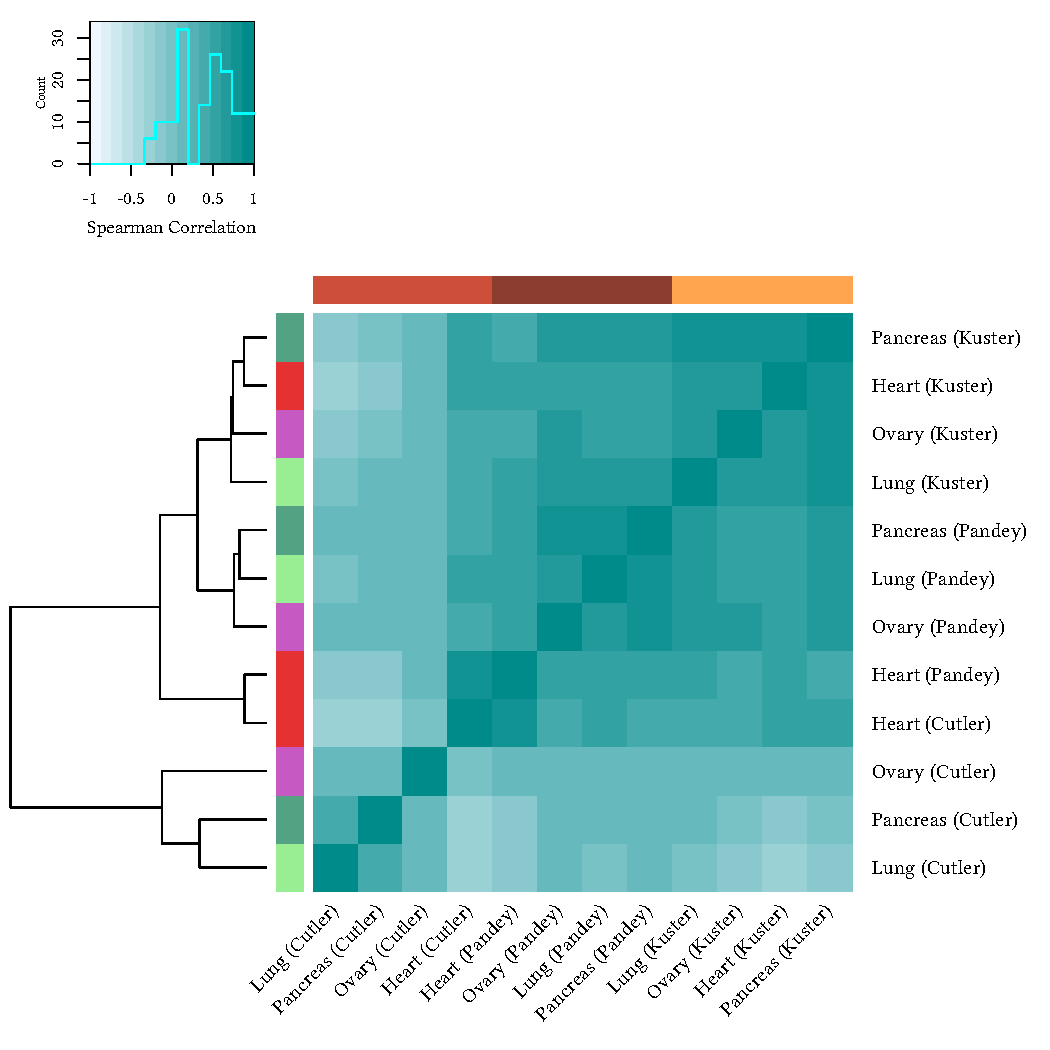
\includegraphics[scale=0.9]{proteomics/heatmap3DproteinSpearman.pdf}\centering
    \caption[Heatmap of the four common tissues between the three proteome
    datasets]{\label{fig:prot3Dheatmap}\textbf{Heatmap of the four common tissues
    between the three proteome datasets} based on
    the pairwise Spearman correlations clustering of 1,384 proteins expression levels.
    Only \heart\ from \cutler\ Lab and \pandey\ Lab have a stronger intratissue correlation
    than an intrastudy one.
    Both for \pandey\ Lab and \cutler\ Lab,
    \pancreas\ and \lung\ are more correlated to each other and their pair to \ovary.
    The heatmap (\Cref{fig:prot3DheatmapPears})
    based on Pearson correlation instead prompts globally identical observations.
    See also \Cref{fig:scat3DheartCutlerPandey} that shows (as a scatterplot)
    the relationship for \Heart\ between \pandey\ Lab and \cutler\ Lab, and then,
    \Cref{fig:scat2DPlacentaKusterPandey} between
    \pandey\ Lab and \kuster\ Lab.
    }
\end{figure}

Following a similar approach to \Crefp{fig:noMitoNoRep4T},
I cluster the twelve proteomic \treps\footnote{See~\Vref{def:trep} for \treps\ definition.}.
I have used Ward's method to link the \treps\ based on their similarity that
I have computed by substracting from 1 the pairwise Spearman correlation
of the expression levels of the 1,384 common proteins.
As shown in \Cref{fig:prot3Dheatmap},
the technical variability overcomes the biological signal
as the proteomic \treps\ cluster according to their original laboratory/study
rather than their biological source,
except for \cutler\ Lab and \pandey\ Lab \heart.
However,
\cutler\ Lab and \pandey\ Lab share the same organisation of their remaining tissues:
\pancreas\ and \lung\ are the most correlated,
and their pair is in turn most correlated to \ovary.
\kuster\ Lab \treps\ display the greatest amount of study bias
(probably due to stronger batch effects --- see \Cref{sub:BatchEffect}).

Removing the proteins translated from the mitochondrial genes slightly
improves the results
but excluding the three ubiquitous (likely contaminants) proteins, presented
in \Cref{subsec:halfProtConfirmed},
is impactless.

Because of the limited number of proteins included in this analysis,
it is unwise to draw definite conclusions
except that there is an extensive need for new quantification normalisation methods
that can help with protein expression meta-analyses
and as for now one has to be very cautious when comparing proteome samples.

I attempted to expand this analysis by comparing the fourteen common tissues
of \pandey\ Lab and \kuster\ Lab datasets,
but the results are as inconclusive
(see \Cref{fig:prot2DheatmapT14,fig:prot2DheatmapPearson}).

\section{New quantification method}\label{sec:NewQuantProt}

In this thesis context where I aim to integrate
the \mRNA\ expression levels to the protein ones
(presented in \Cref{ch:Integration}),
I have developed a new method to infer and quantify the proteins
with the help of \james.

Our original processing workflow (detailed in \Cref{subsec:msDataProcess})
intends to provide a reliable protein quantification.
Our method seems more rigorous than \citet{PandeyData} original paper;
\citet{Ezkurdia2014-qx} challenge the correctness of their quantification
by highlighting the disputable presence of \glspl{OR} in many tissues.
On the other hand, our workflow lacks to detect or quantify any possible \gls{OR}
in the \pandey\ Lab data.
The left part of \Cref{fig:newQuantProtMeth} summarises
our first method of quantification.

\begin{figure}[!htbp]
    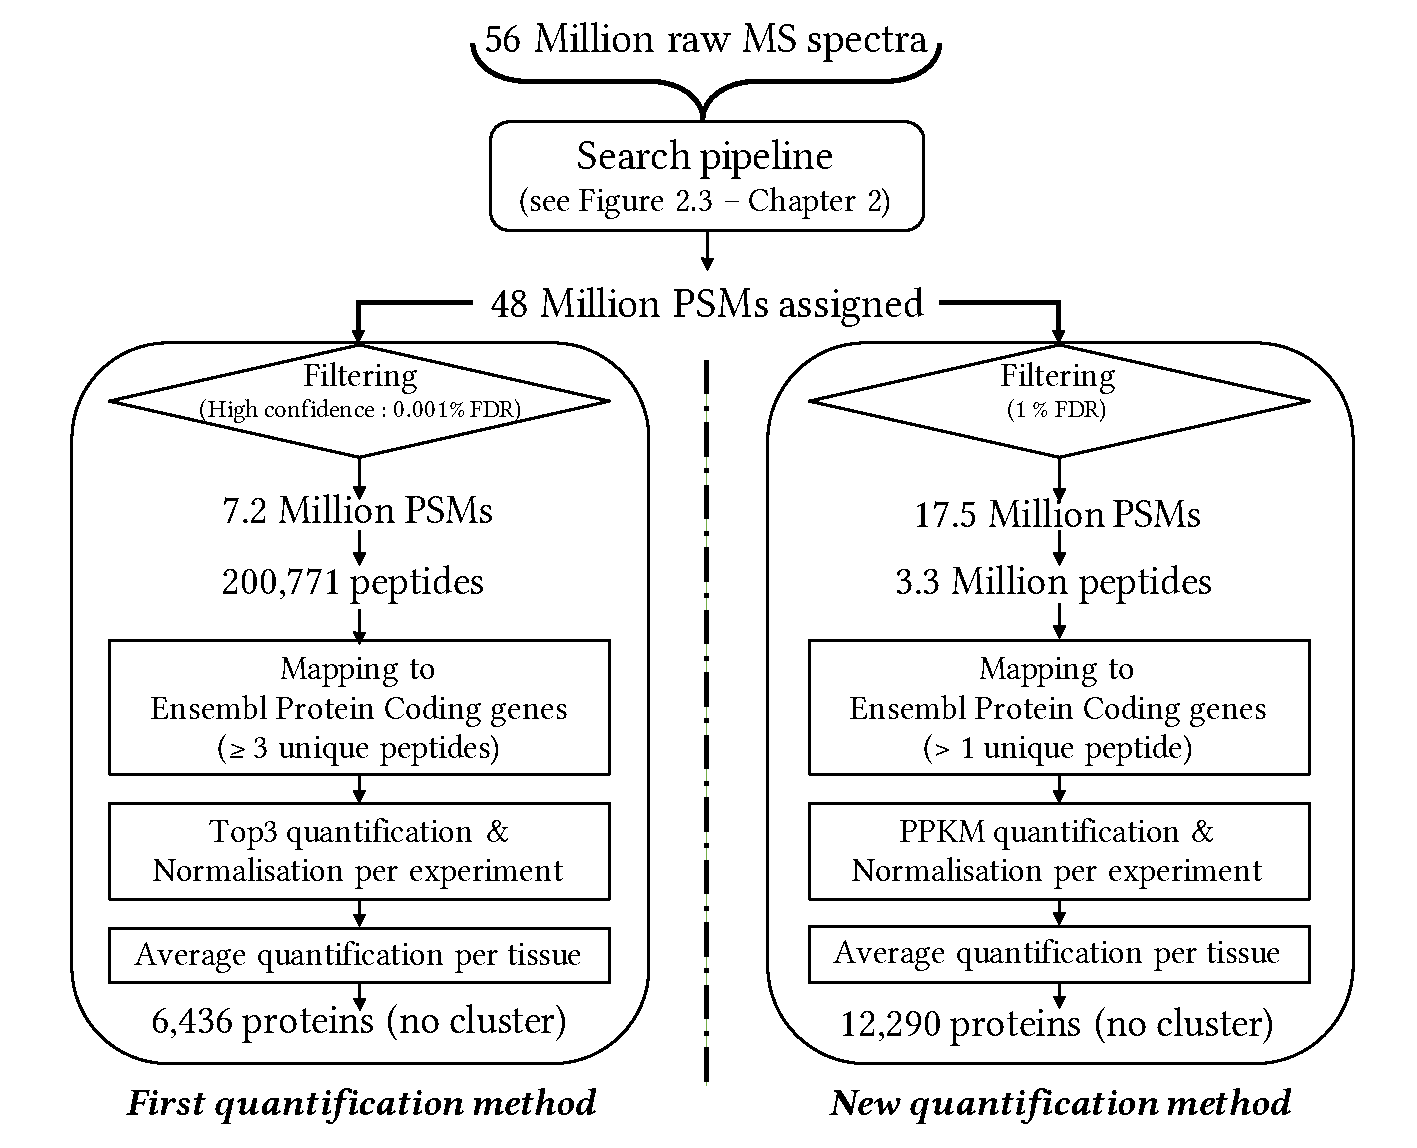
\includegraphics[scale=0.7]{proteomics/quantificationQ1Q2.pdf}\centering
    \caption[Two quantification methods for Pandey Lab data]{\label{fig:newQuantProtMeth}\textbf{Two
    quantification methods for Pandey Lab data.}
    For both approaches, the search pipeline assigning \psms\ remains identical
    (see \Cref{subsec:msDataProcess}).
    The first quantification method,
    which follows a robust inference method
    involving at least three unique peptides,
    relies on the intensity of the three most intense unique peptides.
    The new quantification method that I have devised
    allows more relaxed inference parameters
    as it also uses the non-unique peptides for the quantification.
    See \Cref{eq:PPKM},
    which is similar to \Vref{eq:rpkm-fx}.
    After averaging per tissue and removing the clusters,
    the number of quantified proteins with the new method
    is close to twice the number provided by the first described method.
    The new quantification method was designed
    for the analyses in \Cref{ch:Integration} in particular;
    this is why the filtering is also less strict than for the first quantification method
    since my main focus is the integration of the proteomic data
    with the \Rnaseq\ data.
    Clusters are protein groups that can be mapped to
    more than one \gls{Ensembl} gene identifier.
    Note that the final proteins numbers include only the fifteen tissues
    used for the integration in the following \Cref{ch:Integration}.
    }
\end{figure}

While probably more accurate,
our first quantification is also more stringent than the original one.
Thus, the total number of quantified proteins is more limited.
The requirement of three unique peptides to identify and quantify the proteins
appears to me as the obvious main limiting factor of our method.
As presented in \Cref{ch:background},
the protein quantification relies on
\psms\ identification (see \Cref{subsub:peptideID})
and the chosen approach to infer the proteins (see \Cref{subsec:proteinInference}).
Our first method infers proteins from sets that comprise at least three unique peptides.
The quantification relies on a Top3 approach~\mycite{Silva-Top3}.
It uses the three \emph{unique} most expressed peptides of a protein
to estimate its overall expression
(see \Cref{eq:Top3} (\vref{eq:Top3}) and \Cref{subsubsec:protQuantLB}).

\begin{minipage}{\textwidth}
\begin{equation}
    \tag{Top3 \gls{IBAQ}}\label{eq:Top3}
    \hat{\mu}_{ij}=\frac{\sum \text{Intensity of Top 3 unique peptides} _{ij}}{\text{Total Intensity in experiment } j}
    \raisetag{3\normalbaselineskip}
\end{equation}

where:{\small
\begin{itemize}[topsep=0pt,nosep]
    \item $\hat{\mu}_{ij}$ is the normalised expression for the protein $i$ in experiment $j$ (normalised \gls{PSM}),
    \item $\sum \text{Intensity of Top 3 unique peptides} _{ij}$ is
        the sum of the intensity of the three most intense unique peptides
        of the protein $i$ (mapped to its gene definition $G_i$),
    \item $\text{Total Intensity in experiment } j$ is the total sum of the intensity of all
the peptides identified in the experiment $j$.
\end{itemize}
}
\end{minipage}

The new method I have devised uses both the unique and
the \emph{degenerate} (\ie\ non-unique) peptides
for the quantification step.
It allocates the degenerate peptides
in proportion to the distribution of unique peptides per protein
following a similar approach to \cuffl\ for \Rnaseq\ data (see \Cref{minisec:Cufflinks}).
As three unique peptides are no longer required for the quantification,
it allows relaxing the inference parameters to two unique peptides
(in order to still avoid \emph{one-hit wonders}, see \Cref{subsec:proteinInference}).
The new quantification follows a similar approach to the \RPKM\ normalisation ---
see \Cref{eq:rpkm-fx}.
Protein expression levels are expressed in \glspl{PPKM},
which stands for \glspl{PSM} Per Kilobase of gene per Million.

As shown in \Cref{eq:PPKM},
this method counts the number of \psms\
that can be mapped to the corresponding \gls{Ensembl} gene identifier of a protein.
Then, this raw count is normalised by dividing it
by the product of the longest transcript length and the total number of \psms\
assigned in that experiment;
the result is finally multiplied by a factor ($10^6$) to facilitate reading.
Using the longest \emph{transcript} length
instead of the longest protein isomer allows avoiding issues due to
annotation differences between gene and protein levels
in the analyses of the following \Cref{ch:Integration}.

\james\ has implemented this new method and provided me
\PPKM\ quantifications for the \pandey\ Lab data.

\begin{minipage}{\textwidth}
\begin{equation}\label{eq:PPKM}
    \tag{PPKM definition}
    \hat{\mu}_{ij} = \frac{\text{Number of \psms\ matching } G_i \cdot10^{-6}}{\ell_{G_i}\cdot\sum \text{\psms}_j}
\end{equation}

where:{\small
\begin{itemize}[topsep=0pt,nosep]
    \item $\hat{\mu}_{ij}$ is the normalised expression of the protein $i$
        in the experiment $j$,
    \item $\text{Number of \psms\ matching } G_i$ is the number of \psms\ mapped
        to the definition of the gene $G_i$ that corresponds to the protein $i$,
    \item $\ell_{G_i}$ is the length of the longest transcript of the gene $G_i$,
%\text{Longest transcript length for } G_i$
    \item $\sum \text{\psms}_j$ is the total number of \psms\ identified in
the experiment $j$.
\end{itemize}
}
\end{minipage}

Although smaller,
another limiting factor is the filtering threshold of the selected \psms\
to be inferred in proteins.
We have chosen a conservative (and state-of-the-art) threshold prior to
the first quantification filtering
and a less strict one for the new method.
As my aim is to compare and integrate proteomic and transcriptomic data together,
an increased number of false positives among the identified proteins
(see \Cref{subsub:peptideID}) is not a real issue.

\begin{figure}[!htbp]
    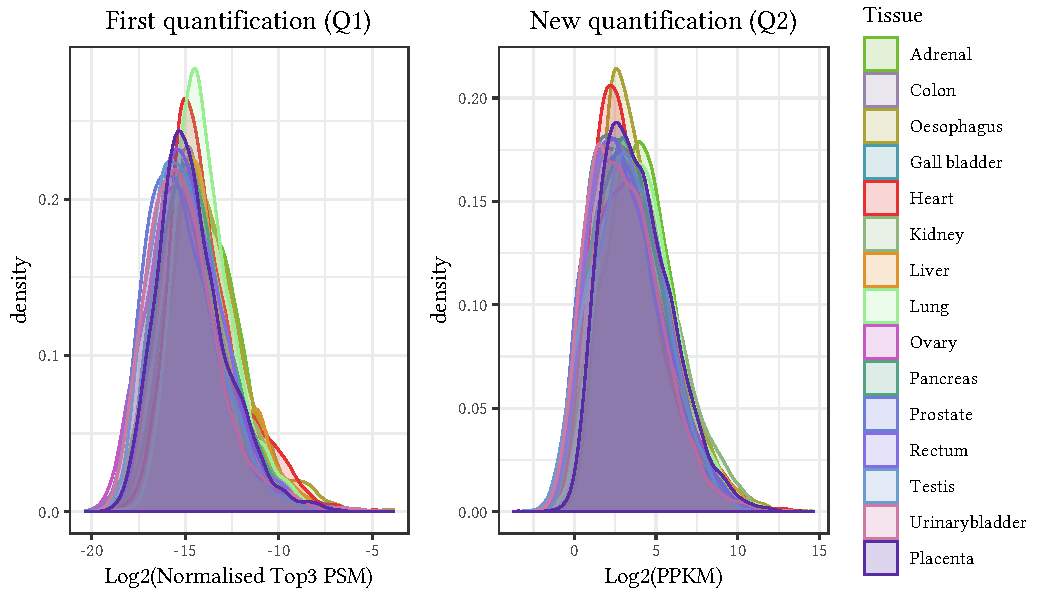
\includegraphics[scale=0.7]{proteomics/distribPandeyQ1Q2.pdf}\centering
    \vspace{-2mm}
    \caption[Pandey Lab data protein expression distribution
    with two quantification methods]{\label{fig:pandeyDistribQ1Q2}\textbf{Distribution
    of the protein expression levels with two different methods.}
    On the left, the protein expression levels distribution for the adult
    tissues of the \pandey\ Lab data with our first quantification method
    (described in \Cref{subsec:msDataProcess}).
    This figure is similar to \Cref{fig:distribProt}(c) but without the fetal tissues.
    On the right are the protein expression levels of the same tissues that
    have been computed with the new quantification method.
    The overall shape of the density plots is very similar between the two approaches.
    }
\end{figure}

Before moving on to the integration of the proteomic and transcriptomic data
in the next chapter,
I have carried out a few comparisons
between the first and the new quantification methods.
As shown in \Cref{fig:pandeyDistribQ1Q2},
the densities of distribution of protein expression levels per tissues
have similar shapes between the two methods.

\Cref{fig:pandeyQ1Q2comp} presents the number of quantified proteins per tissue.
The new method allows quantifying for some tissues
up to more than twice the number quantified by the first method.
This proportion is consistent with the total number of proteins identified
across the fifteen adult tissues
by the first method (6,436)
and the new one (12,290).

\begin{figure}[!ht]
    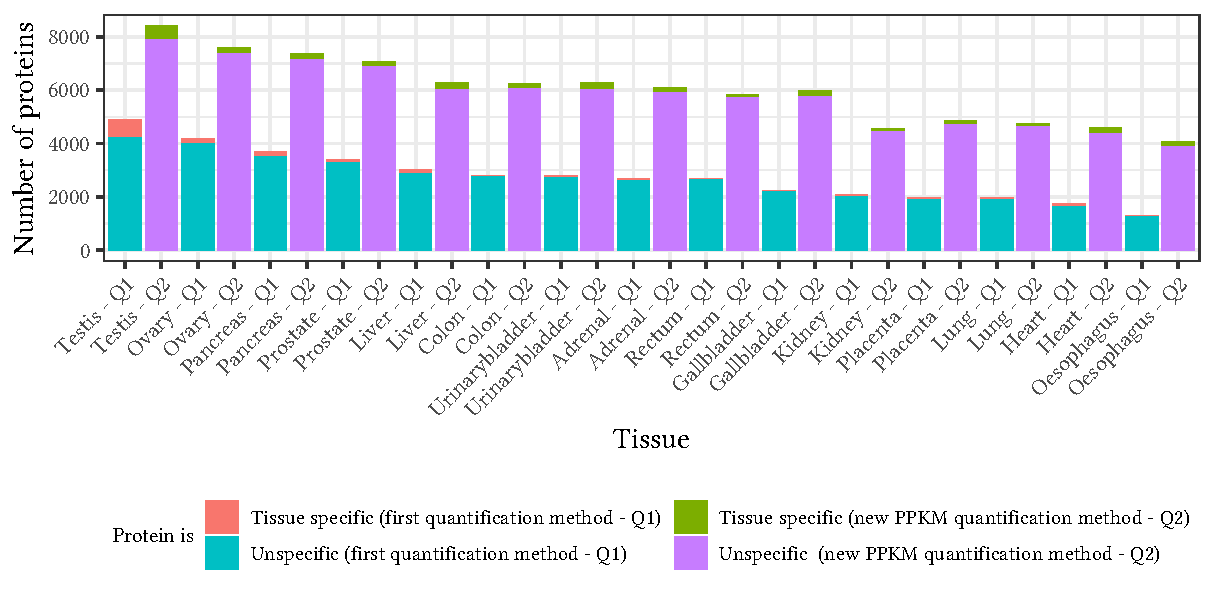
\includegraphics[scale=0.82]{proteomics/compDistribQ1Q2pandey.pdf}\centering
    \vspace{-3.5mm}
    \caption[Comparison of the impact of the quantification method on the
    protein distribution per tissue for Pandey Lab data]{\label{fig:pandeyQ1Q2comp}\textbf{Comparison of
    the impact of the quantification method on the protein distribution per tissue
    for the Pandey Lab data.}
    This figure partly reproduces the \emph{Pandey Lab} part
    of \Cref{fig:distribProtUniq3D}.
    Indeed, the turquoise/red $Q1$ bars are the adult tissues of the \pandey\ Lab data
    quantified with the first quantification method
    (described in \Cref{fig:distribProtUniq3D}).
    The purple/green bars $Q2$ bars are their equivalent
    for the new quantification method.
    The new method allows a considerable increase of
    the identified and quantified proteins number,
    sometimes more than twice as many than the first quantification.
    On the other hand, the rank orders of the total and unique protein numbers per tissue
    are quite similar between the two methods.
    }
\end{figure}

I have also checked the presence of \gls{OR} in the \pandey\ Lab data
with the new quantification method;
only two \glspl{OR} are present:
\protein{OR1M1} in \Kidney\ and \protein{OR13C4} in \Liver.
Their presence may be artefactual, or it may be an issue with the annotation.
Indeed, while these two proteins are missing from all tissues
--- either at \RNA\ or protein levels
--- in \WebFoCi{The Human Protein Atlas}{https://www.proteinatlas.org/}{Uhlen2015},
their \mRNAs\ are present
in the \emph{Baseline expression} of \WebFoCi{\egxa}{https://www.ebi.ac.uk/gxa/}{EBIgxa}
in the human \textit{Chloroid plexus} at 10 post-conception weeks
(HDBR developing brain --- \ArrayExpress{E-MTAB-4840})
and in one sheep \testis\ sample (\ArrayExpress{E-MTAB-3838}).
In addition, \protein{OR1M1} seems to be expressed in the \textit{Blood} of
the green monkey (\species{Chlorocebus sabaeus} --- \ArrayExpress{E-MTAB-4404}).
Both proteins are also found to be up or down regulated at transcript level
in different tumoral samples (\emph{Differential expression} tab of \egxa).
See also the digital supporting data.


%\FloatBarrier

\section{Discussion and Conclusion}

In this chapter, I have reviewed the reprocessed human proteome data
presented in \Cref{ch:datasets},
includes \citet{PandeyData,KusterData}.
Currently, state-of-art bottom-up label-free \ms\ proteomics captures
human tissues expression as a fragmented and disparate universe.
Our processing pipeline (see \Cref{subsec:msDataProcess})
appears more reliable than some of the original authors'.
The original \pandey\ Lab data was disputably quantifying \glspl{OR} in many tissues
\mycite{Ezkurdia2014-qx}.
No trace of \glspl{OR} was found in any of our reprocessed data.\\
\vspace{-\baselineskip}

Nonetheless, the technical variability is overall stronger
than any biological interstudy signal even for similar tissues.
Besides, across the different tissues,
about half of the proteins are consistently observed in the same tissues at least in two datasets.

Even when limited to the protein identification only,
the general lack of repeatability and reproducibility
has been well reported and described
for technical and biological replicates in \ms\ proteomics
(\eg\ \citet{Tu2014-yj,Tabb2010-ro}).
\citet{Canterbury2014-oi} report that
the intra-assay variation between two technical replicates for complex mixtures
can be at least 50\%;
different runs of the same sample or experiment are often produced to raise
the interstudy results repeatability and confidence.\\
\vspace{-\baselineskip}

While there is a definite need for new \ms\ protocols and quantification methods
for baseline expression\footnote{Normalisation methods for differential expression
analysis are usually unsuited for baseline expression studies.
See \citet{Valikangas2018-yj} for possible differential expression quantification
methods.} to correct the extreme variability
and ease the integration of proteomics data from different studies,
I have devised a new quantification method inspired by the \Rnaseq\ ones and
which was implemented by \james.
This new approach (\gls{PPKM}) quantifies
about twice as many proteins than the first one (Top3~\mycite{Silva-Top3}) we used.
\citet{Nesvizhskii2003-ls} propose a method that seems alike,
but their method apportions the degenerate peptides
among all corresponding proteins to estimate their presence likelihood in an experiment.
They focus on the identification while the quantification remains overlooked.

Previously, \citet{Liu2014-xr} had compiled a list of 627 \gls{TS} and
1,093 housekeeping proteins
from the expression data released originally by \citet{PandeyData}.
The data processing has a significant impact on protein identification;
in our first version of \pandey\ Lab data,
I have found 534 housekeeping (ubiquitous) proteins and 1,491 \gls{TS} proteins,
and for the \PPKM\ quantification: 2,057 ubiquitous and 2,640 \gls{TS} proteins.
I provide as digital supporting data the list of the \gls{TS} and
ubiquitous proteins.


%\chapter{Additional}


These will be put at different places in the previous chapters.

\begin{figure}
    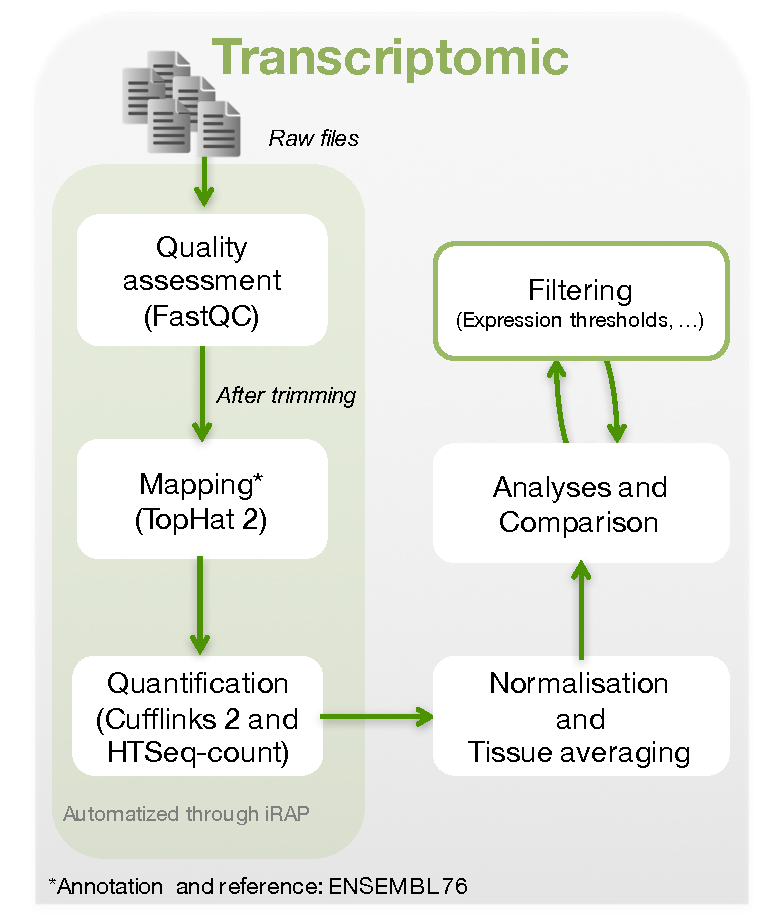
\includegraphics[scale=0.75]{additional/pipelineTrans.pdf}\centering
    \caption[General steps for processing the transcriptomic
    data]{\label{fig:pipelineTrans}\textbf{General steps for processing the
    transcriptome} [TK]}
\end{figure}

\begin{figure}
    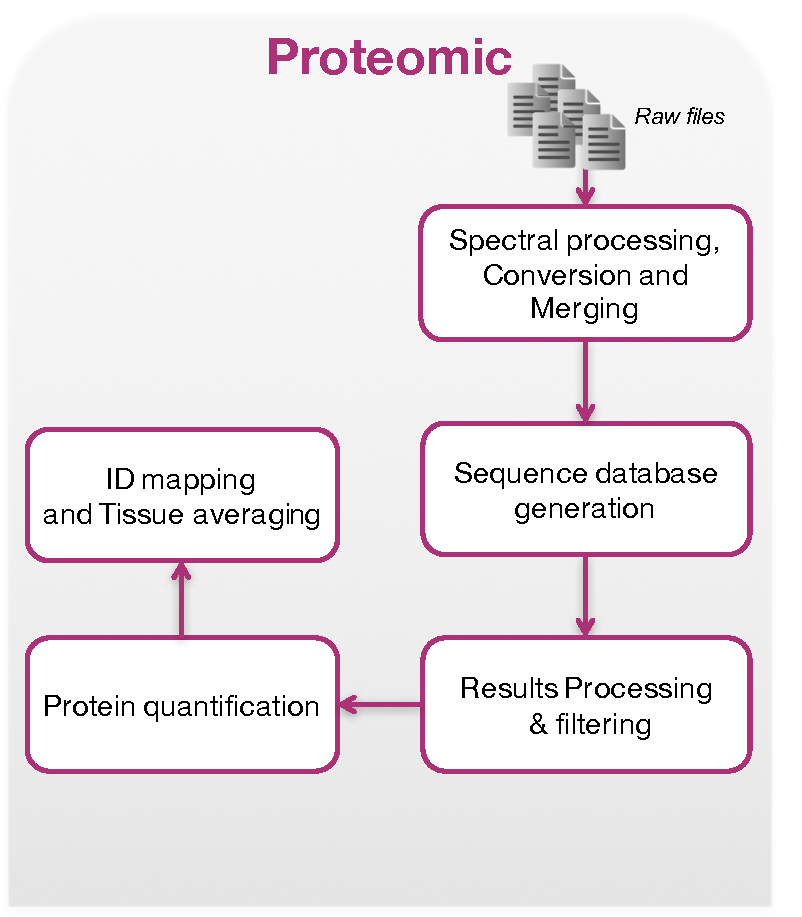
\includegraphics[scale=0.75]{additional/pipelineProteins.pdf}\centering
    \caption[General steps for processing the proteome
    data]{\label{fig:pipelineProt}\textbf{General steps for processing the
    proteome} [TK] }
\end{figure}




\chapter{Integration of Transcriptomic with Proteomic data}\label{ch:Integration}
\setlength{\epigraphwidth}{0.8\textwidth}
\setlength{\epigraphrule}{0pt}
\epigraphhead[5]{%
\epigraph{\emph{Scientists like ripping problems apart, collecting as much data as possible\\
and then assembling the parts back together to make a decision.}}{Shirley M. Tilghman}
}

\vspace{2cm}
After assessing the similarity of the human gene expression profiles
across various tissues
at transcriptomic level (with \Rnaseq\ studies in \Cref{ch:Transcriptomics})
and proteomic level (with \emph{bottom-up} \ms\ studies in \Cref{ch:proteomics}),
my next step is to examine how these gene expression profiles
compare between these two different biological layers.\mybr\

One major aim of this study is to assess
how the correlations between the transcriptome and proteome
described in the literature, mostly measured in cells,
hold at the tissue level.
Moreover, good correlations may potentially lead to
the development of new strategies.
These may use the expression levels of \mRNA\ as proxies
to estimate protein expression,
which is generally difficult to measure directly (see \Cref{sec:exploreProtMS}).\mybr\

I have performed the integration and all the analyses presented in this chapter
under the supervision of \alvis\ and \jyoti.
A manuscript describing this work
and the new method of protein quantification, presented in \Cref{sec:NewQuantProt},
is in preparation.\mybr\

A few closely related studies~\mycite{SciRep2016,Franks2017-bp,Wang2019-ut} have
been published while I was working on
the integration of the non-diseased human transcriptome and proteome.
As their analyses rely on the same data sets (\ie\ \uhlen, \gtex, \pandey\ Lab data)
that I include in my work,
I describe and discuss together my results and theirs
whenever relevant.\mybr\

\clearpage
\derivativeWork{}
\begin{itemize}[topsep=0pt,nosep]
    \item (poster) CSHL  Biology of Genomes 2015 --- A feasibility study:
        Integration of independent human \Rnaseq\ and proteomic datasets
    \item (submitted paper) Mitra P. Barzine, K\={a}rlis Freivalds, James Wemright et al. (2020).
        Using Deep Learning to Extrapolate Protein Expression Measurements.
    \item (submitted paper) Andrew F. Jarnuczak; Hanna Najgebauer; Mitra Barzine;
        Deepti J. Kundu; Fatemeh Ghavidel; Yasset Perez-Riverol; Irene Papatheodorou; Alvis Brazma;
        Juan Antonio Vizcaíno An integrated landscape of protein expression in human cancer
    \item (talk) \gtex\ meeting 2017 --- A. Brazma Correlating transcriptome
        and proteome in human tissues
    \item (poster) HUPO 2018 --- Jarnuczak \etal\ An integrated atlas of
        protein expression in human cancer derived from publicly available
    \item (poster) ECCB 2018 --- Viksna \etal\ An integrated approach
        to missing data imputation in quantitative proteomics experiments
    \item (poster) RECOMB 2018 --- Viksna \etal\ Deep learning
        for protein abundance prediction using Gene Ontology and RNA abundance information
\end{itemize}

\clearpage\

%\vspace{-1cm}

An on-going debate in the literature is
whether good correlations of expression levels prevail
between \mRNAs\ and proteins \mycite{Uhlen:2016}.
The implicit assumption of a proportional relationship is persisting
as the many remaining technological limitations prevent
rigorous testing \mycite{Vogel2012-sq}.
To date, the existence or concentration of a given \mRNA\ transcript
is usually insufficient to ensure detection of the protein in a sample.\mybr\

On the one hand,
\citet{Ramakrishnan2009-lv} report that
\mRNAs\ abundance are roughly sufficient to predict
the protein presence or absence from a sample and
\citet{Vogel2010-ux} that
\mRNA\ level estimations and sequence features are enough to predict
two-thirds of the human protein abundance variation.\mybr\

On the other hand,
the literature fails to report any high correlation
between the transcriptome and the proteome for any organism.
Previous investigations found low or no correlation
between the measured expression profiles of the \mRNAs\ and
proteins in human~\mycite{Anderson1997-le,Chen2002-ob,Tian2004-hh,Pascal2008-gh,%
Gry2009-zv,Lundberg2010-gk},
other mammals~\mycite{Ghazalpour2011-nb},
and across many other species~\mycite{Gygi1999-fl,Maier2009-pb,Maier2011-tz,%
Yeung2011-sl,Palmblad2013-ji,Freiberg2016-fu}.\mybr\

In their encompassing reference experiment,
Schwanhäusser \etal{}~\mycite{schwanhausserglobal:2011,Schwanhausser2013-et}
present rather moderate correlations ($r^2≤0.41,\ie~r<0.64$)
and highlight that \mRNA\ levels explain only about 40\% of protein variations
they have observed.\mybr\

Other studies have explored the \mRNAs\ and proteins relationship in answer
to stimuli~\mycite{Marguerat2012-sn}
or with an increased focus to post-transcriptional regulations
(including degradation rates)~\mycite{Jovanovic2015-wv}.
While many other regulatory processes may occur
(\eg\ translation rates),
post-transcriptional modifications and technical noise
are (still) perceived as the probable primary sources
of \mRNA/protein concentration discrepancies~\mycite{Vogel2012-sq,Plotkin2010-ug}.\mybr\

Joint studies of transcriptome and proteome have already helped to highlight
links between genotype and phenotype~\mycite{Vogel2012-sq}.
However, the mitigated results reported above may explain
the focus shift of many subsequent studies.
While previous efforts were about linking the actual expression levels,
more recent studies primarily have mostly compared qualitative attributes
of given proteins and related \mRNAs{}.
Examples include the comparison of
the presence or absence of \mRNAs\ and their proteins
in specific conditions or tissues~\mycite{Santos2015-rj,Freiberg2016-fu,Uhlen2015}
or the comparison of their differential expression profiles
across identical sets of conditions~\mycite{Varemo2015-uk}.\mybr\

All (or almost all) aforementioned studies have turned to cells
for their joint analyses of transcriptome and proteome.
In contrast,
the analyses and integration I present in this chapter are
based on tissue studies.\mybr\

%\vspace{-2mm}
\section{Data~and~principal~analytical~approaches}\label{sec:IntegrationData}
%\vspace{-4mm}
Since the human proteome drafts~\mycite{PandeyData,KusterData} in 2014,
we have an unparalleled availability of large-scale tissue studies
both at the transcriptomic and proteomic layers to explore and integrate together
(see \Cref{ch:datasets}).
While these data are independent
(collected from various individuals, prepared,
and characterised by different laboratories),
their combined study may help
to shed light on the relationship
between the transcriptome and proteome at the tissue level.
Using different sources for the transcriptome and proteome
increases the overall technical noise,
but it may also help to highlight relevant biological signals (as
they need to be stronger than the noise and batch effects to be captured).\mybr\

In \Cref{ch:Transcriptomics}, I show that
the transcriptome \Rnaseq\ datasets present high interstudy tissue correlations
(median value for Pearson: $r_{\setOneMath}=0.75$; $r_{\setTwoMath}=0.85$ ---
Spearman: $\rho_{\setOneMath}=0.88$; $\rho_{\setTwoMath}=0.93$).
For this chapter analyses,
I only consider the datasets with the highest similarity
(highest correlations)
that incidentally comprise the greatest number of tissues
and are the two most recent studies,
\ie\ \dataset{Uhlén \etal}~\mycite{Uhlen2015}
and \gtex{}~\mycite{GTExTranscript} data.\mybr\

To compensate for the shortfalls in the study design implied
by the reuse of published data\footnote{%
Independent data also means
different collection and sampling processing methods and
lack of information on the samples population background.},
I use both \uhlen\ \etal\ and \gtex\ data
to filter out \mRNAs\ with high interstudy variability for identical tissues.
Whether this variability is technical or biological is irrelevant;
in both cases,
interpreting the relationship
between a highly variable \mRNAs\ and its protein from another dataset
remains hard to interpret.
For these \mRNAs,
it is impossible to explain the observed variability
between the two transcriptomic datasets.
Indeed, any result is subject to the transcriptomic dataset chosen
for the comparison with the proteomic one.
Furthermore, the comparison of the two transcriptomic data may give a reference,
\ie\ an ideal case scenario, for the proteomic/transcriptomic one.\mybr\

On the other hand,
as shown in \Cref{subsec:protTechVarHigh},
the technical variability prevails over
the biological signal of same-tissue samples
for the available high-throughput proteomics.
With the current technological state,
different tissues from the same proteomic study are more likely
to present a higher correlation
than the same tissues from two different studies.\mybr\

To avoid an overly restricted protein set for the following analyses,
I only include one proteomic study: \pandey\ Lab~\mycite{PandeyData}.
All its samples have been run through the same \ms\ platform and
with the same protocol.
Moreover, it presents more homogeneous protein distributions
(see \Cref{fig:distribProt} and \Cref{fig:pandeyDistribQ1Q2}) and
quantifies more proteins per tissue (\Cref{fig:distribProtUniq3D})
than the two other datasets.
Since a current major limitation of bottom-up \ms\ proteomic studies
is the possible lack of detection of proteins for various reasons
(see \Cref{subsec:simpleProt}),
the higher number of detected proteins in \pandey\ Lab data suggests that
this dataset has a higher quality than the two others.\mybr\

%Many strategies are recommended to increase the depth of the coverage
%(\eg\ \mycite{Zhang2014,Eriksson2007-si,Koziol2013-si}).
%Put together, these facts suggest that
%the \pandey\ Lab data has a higher quality than the two other datasets.
%\vspace{-0.5mm}

Though I include one proteomic dataset only,
as the literature reports that
the proteome is more conserved than the transcriptome
(across individuals and species)~\mycite{Laurent2010-rg,Liu2016-re},
this data collection ought to provide
a crude estimate of the extent of observations
that hold from cell to tissue level.\mybr\

This chapter integrates and analyses the matching pairs of \mRNA/proteins
of the common set of tissues between \pandey\ Lab
and the two transcriptomic datasets.\mybr\

\subsection{Overlapping set of tissues for the three datasets}

\begin{figure}[!htbp]
    \includegraphics[scale=0.69]{integration/PandeyGtexUhlen_tissuesVennm.pdf}
    \centering
    \caption[Number of shared and unique tissues between the proteomic
    dataset from Pandey Lab and the transcriptomic datasets (Uhlén \etal\ and
    Gtex)]{\label{fig:VennTissuePandeyGtexUhlen}\textbf{Number of shared and unique
    tissues between the proteomic (Pandey Lab) and the
    transcriptomic (Uhlén \etal\ and GTEx) data.} %The twelve common tissues of
    %the three datasets are
    %\tissue{Adrenal gland}, \tissue{Bladder}, \tissue{Colon}, \tissue{Oesophagus},
    %\tissue{Heart}, \tissue{Kidney}, \tissue{Liver}, \tissue{Lung}, \tissue{Ovary},
    %\tissue{Pancreas}, \tissue{Prostate} and \tissue{Testis}. The three added
    %tissue between \dataset{Uhlén \etal} and \dataset{Pandey Lab} are
    %\tissue{Gall bladder}, \tissue{Placenta} and \tissue{Rectum}. The added tissue
    %between \dataset{GTEx} and \dataset{Pandey Lab} is the \tissue{Frontal
    %cortex}.
    }
\end{figure}

All analyses include the twelve tissues shared between the three
datasets (\adrenal, \Bladder{}\footnote{May also
be referred to as \tissue{Urinary Bladder}},
\hColon, \Oesophagus, \Heart,
\Kidney, \Liver, \Lung, \Ovary, \Pancreas,
\Prostate\ and \Testis).\mybr\

In a few cases, I have also extended the analyses
to three additional tissues (\ie\ \Gall, \Placenta\ and \Rectum)
by including the \uhlen\ \etal\ data on the transcriptomic side only.\mybr\

\subsection{Matching pairs of mRNAs and proteins}
To avoid unnecessary biases (described in \Cref{sec:bias_sources}),
I only consider the \mRNAs\
(\ie\ \glspl{RNA} with a \emph{protein-coding} biotype --- \ens{76})
for the following analyses.
Moreover, since missing data is common for proteomics~\mycite{Lazar2016-oe},
only proteins that are detected in each dataset
in at least one of the included tissues
are considered for further analyses.\mybr\

Besides,
while in the transcriptomics studies
biological replicates of each tissue have been processed
as individual \Rnaseq\ libraries,
in the proteomic one,
the biological replicates have been pooled per tissue before any \ms\ profiling.
Thus, to prevent an unbalanced number of samples biasing
the integration analyses (see \Cref{ch:expression}),
I use \enquote{virtual references},
\ie\ \treps\footnote{\trep{}: \glsdesc{TREP}}
that I computed for each tissue
by taking the median values of each gene
across the biological replicates
(see \Cref{subsec:averagedTissue}).\mybr\

As exposed in \Cref{ch:datasets,ch:proteomics},
all the proteomic quantifications have been provided by \james.\mybr\

The first quantification follows state-of-the-art practices
with stringent parameters (described in \Cref{subsec:msDataProcess})
since accurate protein identification is paramount
for reliable proteome exploration.
The protein levels are given in \glspl{PSM}.
\Cref{fig:PGU_vennQ1} presents
the genes overlap across twelve shared tissues
between the \pandey\ Lab's proteins quantified through this first method
and \uhlen\ \etal{}'s and \gtex{}'s \mRNAs\ quantified
with \htseq\ (see \Cref{subsubsec:RnaseqDataProc}).
\Cref{fig:PU_vennQ1} is the same analysis across the fifteen shared tissues
between \pandey\ Lab and \uhlen\ \etal\ data.\mybr\
\vspace{5mm}

\begin{figure}[!htb]
    \includegraphics[scale=0.65]{integration/PandeyGtexUhlen_mRNAprotQ1Vennm.pdf}\centering
    \caption[Distribution of the unique and shared proteins/mRNAs for the three datasets
    across twelve tissues]{%
    \label{fig:PGU_vennQ1}\textbf{Distribution of the unique and shared proteins
    of Pandey Lab data and mRNAs from Uhlén \textit{et al.} and GTEx ones across
    their twelve shared tissues.}
    There are 6,357 matching gene products between the three datasets.
    Only 5 proteins have apparently no matching partners
    in the \uhlen\ \etal\ or \gtex\ data.}
\end{figure}


\begin{figure}[!htb]
    \includegraphics[scale=0.65]{integration/PandeyUhlen_mRNAprotQ1Vennm.pdf}\centering
    \caption[Distribution of the unique and shared proteins/mRNAs for Pandey Lab
    and Uhlén \textit{et al.} across fifteen tissues.]{%
    \label{fig:PU_vennQ1}\textbf{Distribution of the unique and shared proteins/mRNAs
    for Pandey Lab and Uhlén \textit{et al.} across their fifteen shared tissues.}
    The number of matching pairs (6,428) and proteins that lack a counterpart in
    the transcriptomic data (8) are similar regardless of how many different
    transcriptomic data is included (see \Cref{fig:PGU_vennQ1}).}
\end{figure}

This first proteomic quantification is following robust guidelines,
and both figures show that
almost all the genes with an observed protein
also have an observed \mRNA{}.
However, only about 32\% of the quantified \mRNAs\
in the \uhlen\ \etal\ and \gtex\ data
have a corresponding protein detected in the \pandey\ Lab data.\mybr\

Once I learned more about the bioinformatic challenges of bottom-up proteomics
(described in \Cref{sec:bioinfProt}),
I chose to be more flexible with the identification and quantification methods
to increase the number of proteins included in my analyses.
As I aim to integrate independent proteomics with transcriptomics,
I mostly focus on robust expression between the two biological layers
since discrepancies in this study context are hard to interpret.
While artefacts may persist,
further analyses with targeted proteomics (see \Cref{sec:exploreProtMS})
can help prune or validate the results.\mybr\

I have drawn on \Rnaseq\ transcriptomic approaches to devise
a new quantification method, which is described in \Cref{sec:NewQuantProt}
and implemented by \james.
The method takes advantage of the \emph{degenerate} peptides\footnote{%
See \Cref{subsec:proteinInference}.}
that are distributed across possible protein parents
in proportion to their \emph{unique} peptides.
The method produces normalised values of the protein expression levels
(whose unit is the \gls{PPKM}, \ie\ \glspl{PSM} Per Kilobase of gene per Million).\mybr\

As shown in \Cref{fig:PGU_venQ3,fig:PU_vennQ3},
while the number of quantified proteins
with our new method
covers about 62\% of \uhlen\ \etal{}'s and \gtex{}'s quantified \mRNAs,
the number of proteins for which no \mRNA\ was detected
in the transcriptomic data remains marginal.\mybr\

\begin{figure}[!htpb]
    \includegraphics[scale=0.65]{integration/PandeyGtexUhlen_mRNAprotQ3Vennm.pdf}\centering
    \caption[Distribution of the unique and shared proteins/mRNAs
    across the three datasets and twelve tissues
    (new protein quantification method)]{\label{fig:PGU_venQ3}%
    \textbf{Distribution of the unique and shared proteins/mRNAs
    across twelve shared tissues} between  Pandey Lab
    (\textbf{new quantification method}),
    Uhlén \etal\ and GTEx data.}
\end{figure}

\begin{figure}[!htpb]
    \includegraphics[scale=0.65]{integration/PandeyUhlen_mRNAprotQ3Vennm.pdf}\centering
    \caption[Distribution of the unique and shared proteins/mRNAs
    ahlcross fifteen tissues between Pandey Lab (new quantification method)
    and Uhlén \textit{et al.} data]{\label{fig:PU_vennQ3}\textbf{Distribution of the
    unique and shared proteins/mRNAs across fifteen tissues between
    the Pandey Lab (new quantification method)
    and Uhlén \etal\ data.}}
\end{figure}

Whether it reflects the biological reality or
is solely due to \Rnaseq\ technology being more sensitive than
bottom-up \ms\ alone,
current techniques detect more individual \mRNAs\ than proteins
as confirmed by \Cref{fig:UniqExprPC1,fig:distribProtUniq3D}.
Thus, it may be surprising that
a few proteins lack a match in the transcriptome data.
Several possible explanations exist.\mybr\

Artefacts or technical issues are the most likely.
For example, the annotation might miss
the matching \glspl{RNA} definitions
or defines them with another biotype than \emph{protein-coding}\footnote{%
E.g.\ \gene{XXyac-YRM2039.2} annotated as \textit{unprocessed pseudogene}
and now known as \gene{WASH1} since \ens{77}~(October 2014) or
\gene{TRAJ61} which is annotated as \gene{TR J} \textit{gene}.%
}.
Or, peptides and \mRNA\ reads may be assigned to different gene IDs.
Alternatively, the \mRNAs\ are present in the sample,
but the library preparation has missed their capture
(see \Cref{subsec:libPrep}).
Or even, the presence of proteins in the sample is a false positive
or the result of contamination.\mybr\

However, biological processes might also explain the mismatches.
One example is the case of \mRNAs\ with short half-lives
while their proteins are very stable.
Another possible explanation is that
the original location of the proteins is different
from the tissue in which they were detected
(like hormones or cytokines).\mybr\

Lastly, as the transcriptomic and proteomic samples are independently sourced,
a protein may be specific to an individual or a population.
This last hypothesis is the most unlikely
as there are several biological replicates on the transcriptomic side.
A mixture of the previous causes is also plausible.\mybr\

\begin{figure}[!htbp]
     \includegraphics[scale=0.85]{integration/overviewDatasets1.pdf}\centering
     \vspace{-3mm}
     \caption[Overview of different datasets combination]{%
     \label{fig:setsOverview}\textbf{Overview of different studied datasets
     combinations.}}
\end{figure}

I exclude the unmatched proteins and \mRNAs\ from further analyses.
\Cref{tab:protNoTrans} provides the unmatched protein lists
for the \ens{76} annotation.\mybr\

Unless otherwise stated, to avoid issues exposed in \Cref{subsec:mito},
I also remove all the proteins and \mRNAs\ of the mitochondrial genome
from the subsequent analyses.\mybr\

Note that \Cref{fig:setsOverview} presents
an overview of the various datasets combinations presented
in \Cref{fig:PGU_vennQ1,fig:PU_vennQ1,%fig:VennTissuePandeyGtexUhlen,
fig:PGU_venQ3,fig:PU_vennQ3}.\mybr\

\subsection{Tissue-centric and gene-centric approaches}

\begin{figure}[!htpb]
    \includegraphics[scale=0.85]{integration/VisualExplaination-Lin.pdf}\centering
    %\vspace{-3mm}
    \caption[Summary of the expression comparison approaches between
    the transcriptome and proteome]{\label{fig:visualexp}\textbf{Approaches
    summary of the expression comparison between the transcriptome and proteome.}
    \emph{Tissue-centric} analyses focus on
    how the transcriptome and proteome relate to each other within the same tissue.
    \emph{Gene-centric} analyses study for each gene how its \mRNA\ expression
    levels across all (or a subset of) the tissues may relate to
    the quantified expression levels of its corresponding protein.
    }
\end{figure}

\Cref{fig:visualexp} summarises the two analytical approaches I use
to compare transcriptomic and proteomic data.
The \emph{tissue-centric} approach compares for each tissue
the global expression of its transcriptomic landscape to its proteomic one.
In contrast,
the \emph{gene-centric} approach compares for each gene
its expression levels in \mRNA\ and protein across all the tissues.
\afterpage{\clearpage\sectionmark{Fair correlations between independent proteomics and transcriptomics}}

Confusion can arise
when integrating proteomics and transcriptomics.
Hence, it is essential
to define the taken approach clearly~\mycite{Liu2016-re}.\mybr\

\section{Fair correlations between independently sourced proteomics~%
and~transcriptomics~of~human~tissues~}\label{subsec:IntegrationGoodCorrProtTrans}
\sectionmark{Fair correlations between independent proteomics and transcriptomics}
\vspace{-2mm}

For the first tissue-centric analysis,
I assess for each tissue the relationship between
the expression of its proteome and transcriptome
through the correlation of the protein expression values
with their corresponding \mRNA\ ones.\mybr\

After scaling with $\log_2(x+1)$,
I compare proteomic and transcriptomic \treps\
from identical and random tissue pairs,
which are similar and roughly correspond to Gaussian distributions
as illustrated by \Cref{fig:distribTrans,fig:pandeyDistribQ1Q2}.\mybr\

\Cref{fig:TestSig} presents the correlation distribution range
of transcriptomic and proteomic \treps\ from identical and random pairs of tissues,
both with Spearman and Pearson correlation methods
(see \Cref{sec:CorrMore}).\mybr\

Although transcriptomics and proteomics have independent sources,
the Spearman correlations of the same tissues \treps\ are equivalent to
correlations in cell studies~\mycite{Lundberg2010-gk,schwanhausserglobal:2011}
where the same sample provides \mRNAs\ and proteins.
Regardless of the protein quantification method
(Top3~\mycite{Silva-Top3} or \PPKM{} ---~\vref{eq:PPKM}),
the median Spearman correlation coefficients are above $0.5$
for matched proteomic and transcriptomic \treps\
(also referred to as \emph{same-tissue pairs}).
The unscaled data presents identical outcomes
(see \Cref{tab:pvalueCorrSP} and \Cref{fig:TestSigUnlog}).\mybr\

The Pearson correlation is closer to the literature
for our new \PPKM\ quantification
than for the Top3 quantification.
The \PPKM\ Pearson correlation averages
above $0.5$ $[$min:~$0.38$~(\Oesophagus)\;; max:~$0.61$~(\Liver)$]$
(and is within $[$min:~$0.45$~(\Oesophagus)\;; max:~$0.67$~(\Liver)$]$
for the untransformed data).\mybr\

\begin{figure}[!htbp]
    \includegraphics[scale=0.8]{integration/DFtestlog2.pdf}\centering
    \vspace{-4mm}
    \caption[Distribution of Pearson and Spearman correlation coefficients
    for same-tissue proteomic and transcriptomic pairs
    versus random tissue pairs]{\label{fig:TestSig}\textbf{Distribution of
    Pearson and Spearman correlation coefficients
    for same-tissue proteomic and transcriptomic pairs versus random tissue
    pairs ($\log_2$-scaled data).} Depending on the protein quantification method,
    there are two types of distribution ranges for the Pearson correlations.
    Top3 quantification method provides a lower correlation ($\text{mean} \approx 0.11$).
    The \PPKM\ method (\Cref{sec:NewQuantProt}) produces higher correlations
    ($\text{mean} \approx 0.5$).
    All the Spearman correlation ranges between same-tissue proteomic and
    transcriptomic \treps\ are quite similar,
    regardless of the method quantifying the proteins.
    The median of Spearman correlation is $0.52$.
    With the Top3 quantification (\ie\ pink countered boxes --- Top3 x HTSeq),
    two outliers are noticeable, and they are common to the three comparisons,
    Pandey x Uhlén (12 tissues and 15 tissues) and Pandey x GTEx (12 tissues):
    the lowest Spearman correlation is \Oesophagus\ ($\rho=0.39$)
    and the highest \liver\ ($\rho=0.62$).
    Both for the Pearson and Spearman correlations,
    even when the correlations are very low,
    same-tissue pairs always have higher correlations than
    different (random) tissues pairs
    (all p-values computed with Welch t-test <0.05 --- see \Cref{tab:pvalueCorrSP}).
    Thus, even the lowest same-tissue correlations are significant.
    The green boxplots, comparing the two transcriptomic datasets,
    are only represented for reference purposes.}
\end{figure}

\begin{figure}[!htbp]
    \includegraphics[scale=0.75]{integration/Kidney_scattplot_Q3_T15.pdf}\centering
    \caption[Scatterplot of protein (Pandey Lab data --- PPKM quantification)
    and mRNA (Uhlén \etal) expression for Kidney]
    {\label{fig:ScatKid}\textbf{Scatterplot of
    protein (Pandey Lab --- PPKM quantification) and mRNAs (Uhlén \textit{et al.})
    expression for Kidney.}
    Each point of this scatterplot represents a gene;
    it has the $\log_2$-transformed expression value
    of the corresponding \uhlen\ \etal\ \mRNA\ (\FPKM) on the x-axis and
    the $\log_2$-transformed expression value of
    the \pandey\ Lab protein (\PPKM) on the y-axis.
    Most of the \mRNA/protein pairs are distributed in an area
    that can be fitted by a linear function with a positive slope,
    which indicates a high correlation between \mRNAs\ and proteins expression
    levels.
    However, genes with lower expressed \mRNAs\ have
    a less associated expression between their protein and \mRNA,
    in particular, \mRNAs\ that are expressed
    below $1$ \FPKM\ (\ie\ below $0$ on the x-axis).
    On the other side, genes with the highest expressed \mRNAs\ may present
    a saturation effect (\Cref{subsec:simpleProt})
    in the quantification of the protein expression.
    The highest expressed protein is \protein{\gls{HBB}}
    (\ie\ Hemoglobin Subunit Beta), which is also found in
    the five highest expressed proteins in all the other tissues.
    Possibly, its presence is due to remaining erythrocytes in the samples.
    On the outer parts of the scatterplot,
    there are the respective distribution densities of the proteins and the \mRNAs.
    Whilst the correlation calculation includes every pair of \mRNA\ and protein,
    the plot excludes any pair with an unexpressed \mRNA\ or protein to optimise the visualisation.
    \Cref{fig:scatplotAll} presents an overview of the other tissue scatterplots.
    }
\end{figure}

As tissue proteomic samples can present high correlation
without being related in any manner
(see \Cref{ch:proteomics,fig:scat2DAdrenalPancreasKuster}),
a Welch t-test~\mycite{Welch1951-sj} allows
assessing the significance of the correlation for the same-tissue pairs
by comparison to random tissue pairs.
The one-sided \Welchttest\footnote{See \Cref{mini:ttest}}
allows rejecting the null hypothesis $H_0$
(the means of the correlation coefficients for same-tissues pairs
are identical or lower to random tissues pairs).
Irrespective of the protein quantification or computational methods,
all the same-tissue pairs correlations are significant
(p-value $<5.10^{-5}$, except for Pearson correlation with Top3 quantification
where p-value $<0.05$ --- see \Cref{tab:pvalueCorrSP}).\mybr\

The previous correlation distribution
may imply a modest relationship between
these independent proteomics and transcriptomics,
but the same-tissue pairs scatterplots (\eg\ \Cref{fig:ScatKid})
show tighter links than first suggested.
Besides, these scatterplots share a coarse profile
despite the wide correlation ranges.\mybr\

\Cref{fig:ScatKid} illustrates the comparison of expression for \kidney\
between transcriptomics (\uhlen\ \etal) on the x-axis
and proteomics (\pandey\ Lab --- \PPKM) on the y-axis.
\Kidney's correlation coefficients stand in the middle of the range
regardless of the considered studies,
protein quantification or correlation methods involved in the comparison.\mybr\

%To optimise the visualisation,
%I removed the pairs with a null member
%(either for the \mRNA\ or protein)
%while I keep them for the correlation calculation.


A linear function with a positive slope (not drawn) can fit the bulk of the points.
Indeed, the expression of most \mRNAs\ and proteins in a tissue
are highly associated
with the exception of the lowest ($<1$ \FPKM) and
a number of the highest measured \mRNAs{}.\mybr\

Besides the mismatching sampling sources,
other possible explanations for the observed divergences are
technical limitations (such as protein saturation effect, see \Cref{subsec:simpleProt}),
translational noise (see \Cref{subsubsec:exprTrans})
or a consequent half-life difference between the \mRNA\ and its protein.\mybr\

Although the number of genes
presenting lowly associated levels of \mRNA/protein expression is rather limited,
it is enough to impair the Pearson and Spearman correlation coefficients.\mybr\

Systematic exclusion of lowly associated pairs of \mRNAs\ and proteins
is impractical and arguable
as they are inconsistent from one tissue to another.\label{memo:dispersedGenes}
Case-by-case treatment will be necessary.\mybr\

Removing the lowly expressed \mRNAs\ ($<1$ \FPKM) only marginally changes
the correlation coefficients,
\eg\ for \kidney,
when considering the \PPKM\ quantification for the proteins,
the Pearson correlation
increases from $0.56$ to $0.58$,
while the Spearman correlation is relatively unchanged
($0.51$ instead of $0.52$).
There are similar changes observed
when considering the more conservative Top3 protein quantification.
The Pearson correlation $r=0.18$ increases to $0.21$.
The Spearman correlation remains unchanged ($\rho=0.52$).\mybr\

Both transcriptomic studies (\uhlen\ \etal\ or \gtex)
providing equivalent results,
I describe for most of the following analyses the data combination
that provides the greatest number of tissues and genes to study,
\ie\ the fifteen-tissue set between \uhlen\ \etal\ and \pandey\ Lab data
quantified with the \PPKM\ method.\mybr\

\vspace{-1mm}
The other combinations
(provided in \Cref{ch:SupplIntegration} or electronic format)
may diverge for individual genes through the various combinations,
but the general trends are identical.\mybr\
\vspace{-1mm}

I focus on Pearson correlation over Spearman correlation
in the following parts
since the results for the \PPKM\ quantification are globally similar for both.\mybr\

\subsection{Mixed biological signal between the proteome and transcriptome
across the tissues}
%\vspace{-8mm}
\begin{figure}[!hb]
    \includegraphics[scale=0.85]{integration/orderedHeatmapQ3Pearson1.pdf}\centering
    \vspace{-2mm}
    \caption[Heatmap based on the Pearson correlation between protein and mRNAs
    expression (alphabetically ordered tissue)]{\label{fig:orderedHeatmapPearson}%
    \textbf{Heatmap based on the Pearson correlation between protein and mRNAs
    expression (alphabetically ordered tissue).}
    Correlations for same tissue pairs (diagonal) are highlighted in
    yellow when the highest observed correlations are between the matching proteomics
    and transcriptomics pairs; in dark pink, when the proteomics correlates
    the best with the matching transcriptomics.
    When other higher correlations are observed for a tissue proteomics or transcriptomics
    they are in given grey.}
\end{figure}

As shown in \Cref{fig:orderedHeatmapPearson},
for nine tissues (in yellow) transcriptomic and proteomic expressions correlate
better in matching tissues.
For four other tissues (\hColon, \Lung, \Oesophagus\ and \Urinarybladder\
--- in dark pink),
only the proteomics correlate the best with the matching transcriptomics,
while the transcriptomics correlates better with other proteomics tissues.
The remaining two tissues have their proteomics correlating
as much (\eg\ \Gall) to other tissues or more to transcriptomics
from other tissues (\Rectum).\mybr\

While the different correlation methods lead to similar result trends,
individual differences persist.
In a few cases, \eg\ \heart,
these slight differences may considerably change
the relative correlation ranking order of the \treps{}.\mybr\

In the following sections,
I explore several avenues to identify possible factors
that influence the association strength
between the proteome and transcriptome.\mybr\

I first study the effect of tissue composition (in proteins and \mRNAs)
on the correlations.
I begin with the assessment of the impact of the proteins and \mRNAs\
that are found in one tissue only,
before looking into the tissue-specific (\gls{TS}) proteins and \mRNAs{}.\mybr\

Then, in a more quantitative approach,
I examine more closely how the \mRNA\ expression profiles relate
to their respective protein ones.\mybr\

\subsection{Influence of the expression breadth on the tissue %
\texorpdfstring{\MakeLowercase{m}RNAs/proteins}{mRNAs/proteins} correlation}

In \Cref{ch:proteomics},
I have shown that
the protein expression of both different tissues and same-tissue pairs
are sharing a similar correlation range
(see \Cref{fig:scat2DAdrenalPandeyPancreasKuster}).
In this context,
genes expressed in a small number of tissues
(both as a protein and \mRNA)
can have a significant impact on the correlation
and may explain the mitigated results.\mybr\

The expression breadth of a gene is
the number of tissues and cell lines within which the gene is expressed.
\Cref{fig:expressionBreadth} allows visualising
the distribution of the expression breadth of the \mRNAs\ (\uhlen\ \etal)
and the proteins (\pandey\ Lab data) across their fifteen common tissues.
In the following sections,
I can refer to a (\gls{TS}) gene as a \emph{unique gene}
when it is only expressed in a single tissue.\mybr\

\Cref{fig:protBreadth} shows that
the distribution of the protein expression breadth is bimodal.
Either due to technical limitations or biological reasons,
proteins detected in a sole tissue form
the most numerous class and represent 20 \% of the overall number.
Proteins expressed in all tissues are the second most numerous class (about $~$ 16 \%);
the third largest class (12 \%) comprises the proteins expressed in two tissues.\mybr\

On the other hand,
almost all \mRNAs\ are expressed in every tissue (\Cref{fig:mRNAbreadth0}).
One hypothesis is that \mRNAs\ levels have to exceed a sufficient threshold
for their proteins to be detected.
Thus, I also studied the effect of
two additional minimum expression thresholds for the \mRNAs\
on the expression breadth.\mybr\

The two new expression breadth profiles are more alike
to the proteomic one.
As shown in \Cref{fig:mRNAbreadth1},
the number of transcripts only found in one tissue increases
at the widespread $1$ \FPKM\ threshold,
which roughly equates to one \gls{RNA} in the cell~\mycite{Mortazavi2008,Hebenstreit:2011}.\mybr\

The expression breadth profile of the \mRNAs\ expressed at or above $5$ \FPKM\
present a similar bimodal distribution (\Cref{fig:mRNAbreadth5}) to the protein one.
While arbitrary, $5$ \FPKM\ is a threshold commonly found
in the literature~\mycite{Uhlen2015,oneDominant,Chen2018-ln}.\mybr\

\begin{figure}[!htb]
    \begin{subfigure}[h]{0.53\textwidth}
    \captionsetup{margin=0.6cm,justification=centering}
        \centering \includegraphics[width=\textwidth]{integration/breadthProtQ3--15.pdf}
        \caption{Protein~expression~breadth (\PPKM~quantification)}\label{fig:protBreadth}
    \end{subfigure}
    \begin{subfigure}[h]{0.53\textwidth}
    \captionsetup{margin=0.6cm,justification=centering}
        \centering \includegraphics[width=\textwidth]{integration/breadthmRNAQ3--15.pdf}
        \caption{mRNA~expression~breadth\\(> 0 \FPKM)}\label{fig:mRNAbreadth0}
    \end{subfigure}
    \vspace{2.5mm}

    \begin{subfigure}[b]{0.53\textwidth}
    \captionsetup{margin=0.6cm,justification=centering}
        \centering \includegraphics[width=\textwidth]{integration/breadthmRNAQ3--1501.pdf}
        \caption{mRNA~expression~breadth\\(≥1 \FPKM)}\label{fig:mRNAbreadth1}
    \end{subfigure}
    \begin{subfigure}[b]{0.53\textwidth}
    \captionsetup{margin=0.6cm,justification=centering}
        \centering \includegraphics[width=\textwidth]{integration/breadthmRNAQ3--1505.pdf}
        \caption{mRNA~expression~breadth\\(≥5 \FPKM)}\label{fig:mRNAbreadth5}
    \end{subfigure}
    \vspace{-6mm}
    \caption[Expression breadth of the proteins and mRNAs]{\label{fig:expressionBreadth}%
    \textbf{Expression breadth of the proteins and mRNAs.}
    The expression breadth of the proteins has a bimodal distribution.
    Many proteins are detected either in a single tissue or in all of them.
    Almost every \mRNA\ is detected in every tissue.
    Their breadth becomes bimodal when their expression threshold
    is increased to $5$ \FPKM{}.
    To ease the general visualisation,
    I have omitted to plot the \mRNAs\
    for which the expression remains below the threshold for all tissues
    (\ie\ expression breadth=0 for the considered threshold).
    }
\end{figure}

\Cref{fig:UniqueFeatureQ3T15} displays the fraction of unique genes
(\ie\ only expressed in a single tissue)
detected as a protein or an \mRNA\ at a considered threshold for each tissue as
the analysis is seeking a possible link between
the number of uniquely detected genes
and the correlation strength between the proteomic and transcriptomic \treps{}.
Hence, these fractions are computed by dividing
the number of unique genes (proteins or \mRNAs) of each tissue
by the total amount of uniquely detected genes across all tissues.
The tissues are ordered by increasing order of their fraction.\mybr\

\begin{figure}[!htb]
    \includegraphics[scale=0.78]{integration/uniqueFeatureQ3T15a.pdf}\centering
    \vspace{-5mm}
    \caption[Unique proteins or mRNAs fractions across tissues]{\label{fig:UniqueFeatureQ3T15}
    \textbf{Unique proteins or mRNAs fractions across tissues.}
    }
\end{figure}

Although their proportion varies from one tissue to another,
all fifteen tissues have proteins
that are specifically detected in each tissue solely,
as shown in the top plot in \Cref{fig:UniqueFeatureQ3T15}.
In contrast, unique \mRNAs\ are detected in a more limited number of tissues
(see the three bottom plots of \Cref{fig:UniqueFeatureQ3T15}).
Besides, the unique proteins are more evenly distributed
between the fifteen tissues than the unique \mRNAs.\mybr\

Except for \Testis\ and \Liver,
which are consistently expressing the highest number of uniquely detected genes,
the other tissues fail to present any similarity
between the available proteomic and transcriptomic data.\mybr\

\Liver\ is the most correlated tissue (\Cref{fig:orderedHeatmapPearson})
and comprises the second-highest number of unique genes.
\Testis\ is the third-best correlated tissue
despite having the highest fractions of unique proteins and \mRNAs\
regardless of any threshold.
It may be tempting to hypothesise that the number of unique genes
relate to correlation levels,
but the other tissues fail to show any relationship
between the number of unique \mRNAs\ and proteins they expressed
and the strength of the correlations.\mybr\

Put together, these results suggest that
the number of proteins and \mRNAs{} uniquely expressed in these tissues
play a minor role at best in the \mRNA/protein correlation computed for each tissue.
The lack of relation between the proteomic and transcriptomic observations
is confirmed by a more refined analysis of the expression breadth.\mybr\

\begin{figure}[!htb]
    \includegraphics[scale=0.75]{integration/coloredSharedbreadthProtQ3--15.pdf}\centering
    \vspace{-4mm}
    \caption[Comparison of proteins expression breadth to
    corresponding mRNA breadth]{\label{fig:SharedBreadthProtQ3}%
    \textbf{Comparison of proteins expression breadth to their corresponding mRNA.}
    The proteins' expression breadth (\Cref{fig:protBreadth})
    is coloured according to
    their corresponding \mRNA\ expression breadth at $5$ \FPKM\
    (\Cref{fig:mRNAbreadth5}).
    About one-fifth of the uniquely detected proteins have
    their corresponding \mRNA\ identically expressed once at or above 5 \FPKM{}.
    The number of proteins classified as \emph{Identical} decreases significantly
    through other breadths until it raises again from thirteen tissues
    to reach about one-third of the ubiquitous proteins.
    Proteins and \mRNAs\ with mismatching expression breadth are split into
    several categories.
    Proteins and \mRNAs\ that are both detected within four to twelve tissues
    are described as \emph{Mixed}.
    If the expression breadths of the remaining pairs are close (± $2$),
    they are identified as \emph{Similar} otherwise as \emph{Different}.
    Finally, many genes detected at least once as a protein have
    an \mRNA\ expression that never reaches $5$ \FPKM{} (\emph{Expression < $5$ \FPKM}).
    }
\end{figure}

\Cref{fig:SharedBreadthProtQ3} shows that the expression breadth
of \mRNAs\ (expressed ≥ $5$ \FPKM\ or even smaller threshold) concurs
in very few cases to their corresponding protein breadth.
Thus, the \mRNA\ expression breadth is insufficient
to predict the expression breadth of the corresponding protein.
Even for the two extreme cases
where the protein is unique to a tissue or ubiquitous (found in all fifteen tissues),
there are differences between the expression breadths of the \mRNA\ and the protein
of the same gene.\mybr\

All the expression breadth analyses of the transcriptome rely on expression levels.
However, \Cref{ch:Transcriptomics} underlines that
high \mRNA\ expression levels are unrelated
to high interstudy correlation of same-tissue pairs
while \gls{TS} \mRNAs\ present a rather strong relation with it.
For this reason, the following analysis examines
the relationship between \gls{TS} \mRNAs\ and \gls{TS} proteins.\mybr\


\subsection{Tissue-specific \texorpdfstring{\MakeLowercase{m}RNAs}{mRNAs} %
have significant overlap with tissue-specific proteins}\label{sec:TSprotMrna}

Unlike \mRNAs,
many proteins are only expressed in one unique tissue.
These are the ones I refer to as \gls{TS} proteins in the remainder of this thesis.\mybr\

To enable the comparison of these \gls{TS} proteins with possible transcript partners,
I first need to define a set of \gls{TS} \mRNAs{}.
To find the latter, I choose the $n$ \mRNAs\ most specific to a tissue
based on the \nameref{subsub:TisSpeGeneMethodPerso} (\Cref{subsub:TisSpeGeneMethodPerso})
where $n$ is the number of \gls{TS} proteins of that tissue.
Then, as detailed in \Cref{fig:RankSpe},
I examine for each tissue the overlap between its $n$ \gls{TS} proteins
with its $n$ \mRNAs\ with the highest tissue-specific ranks.
\Cref{fig:ExJacquard} illustrates the \heart\ example.\mybr\

\begin{figure}[!htb]
    \includegraphics[scale=0.59]{integration/TissueSpeDeter1b.pdf}\centering
    \vspace{-3mm}
    \caption[Determination process of the specific mRNAs]{%
    \label{fig:RankSpe}\textbf{Overview of the comparison of the TS proteins
    and TS mRNAs.}
    \gls{TS} proteins are the $n$ proteins only expressed in one tissue.
    Once the \mRNAs\ have been sorted
    by decreasing order of their relative specificity to a given tissue,
    the first $n$ \mRNAs\ identities are compared
    to the ones of the $n$ \gls{TS} proteins present in the same tissue.
    %Jaccard's similarity coefficients and their significance (p-values)
    %are computed to allow
    %a global assessment of the proteome and transcriptome relationship
    %across all the tissues simultaneously.
    }
\end{figure}

\begin{figure}[!htbp]
\includegraphics[scale=0.63]{integration/overlapRatioPUQ15Q3Heart.pdf}\centering
\vspace{-3mm}
    \caption[Example of overlap of TS proteins and TS mRNAs for Heart]{%
    \label{fig:ExJacquard}\textbf{Example of overlap of \gls{TS} proteins
    and \gls{TS} \mRNAs.}}
\end{figure}

Each tissue has a different number of \gls{TS} proteins.
I thus refine this analysis
by computing Jaccard similarity coefficients
(or Jaccard indices)~\mycite{Jaccard1901-ei,Lin2008-fc},
see \Cref{eq:Jaccard}.
The Jaccard indices allow assessing
the relationship between \gls{TS} proteins and \mRNAs\
across all the tissues at the same time
and ease the result interpretation in contrast to the raw overlap numbers.\mybr\

\begin{minipage}{\textwidth}
    The Jaccard index is computed as follow:
\begin{equation}
    \tag{Jaccard similarity coefficient}\label{eq:Jaccard}
    \begin{split}
        J(x_{1},x_{2}) & = \frac{\left | x_{1}\cap  x_{2}\right |}%
                                {\left | x_{1}\cup  x_{2}\right |}\\
                       & = \frac{\left | x_{1}\cap  x_{2}\right |}%
                                {\left | x_{1} \right | + \left | x_{2} \right |%
                                - \left | x_{1}\cap  x_{2}\right |}\\
    \end{split}
    \raisetag{6cm}
\end{equation}

When applied specifically to \Cref{fig:RankSpe}, we get:
$J(\tikzcircle[Tan,fill={rgb,255:red,195; green,160;blue,153}]{4pt},%
\tikzcircle[DarkOrchid,fill={rgb,255:red,215; green,145; blue,254}]{4pt}) = \frac{k}{2n-k}$,\\
with $n$ the number of proteins (\tikzcircle[Tan,fill={rgb,255:red,195; green,160;blue,153}]{4pt})
that are only found in a given tissue and
$k$ is the number of common genes between
these $n$ unique proteins
%(\tikzcircle[Tan,fill={rgb,255:red,195; green,160;blue,153}]{4pt})
and the $n$ most specific \mRNAs\ of the tissue
(\tikzcircle[DarkOrchid,fill={rgb,255:red,215; green,145; blue,254}]{4pt}).
\end{minipage}

\vspace{3mm}
To measure the Jaccard indices significance,
I use the hypergeometric test~\mycite{Field2012-au}
(see \Cref{sec:hypergeometricTest}).
In the current analysis,
I consider as success when a \gls{TS} \mRNA\ is among the $n$ \gls{TS} proteins
and test if the number of observed successes is greater than
the expected number for random sampling.\mybr\

\vspace{3mm}
The Jaccard indices for all pairs of the fifteen shared tissues
between the \pandey\ Lab (\PPKM\ quantification) and \uhlen\ \etal\
are summarised in \Cref{fig:JaccardIndexes},
while~\Cref{fig:JaccardPvalues} displays
their respective p-values (hypergeometric test).\mybr\

\begin{figure}[!ht]
    \includegraphics[scale=1]{integration/overlapRatioPUQ15Q3.pdf}\centering
    %\vspace{-3mm}
    \caption[Heatmap of Jaccard indices across 15 tissues]{%
\label{fig:JaccardIndexes}\label{fig:RatioJac}\textbf{Heatmap of Jaccard indices
across the common fifteen tissues between Uhlén \textit{et al.} and Pandey Lab data.}
For each tissue, the \gls{TS} proteins are the proteins
(quantified with \PPKM\ method) that are expressed only in that tissue.
The \gls{TS} \mRNAs\ are the \mRNAs\ with the highest specific coefficients
in that tissue.}
\end{figure}

\begin{figure}[!ht]
    \includegraphics[scale=1]{integration/overlapRatioPvalPUQ15Q3.pdf}\centering
    %\vspace{-3mm}
    \caption[p-values associated with the Jaccard indices]{%
\label{fig:JaccardPvalues}\label{fig:pJacquard}%
    \textbf{p-values associated with the Jaccard indices} of \Cref{fig:JaccardIndexes}.
    These p-values have been computed with the hypergeometric test.}
    \vspace{-3mm}
\end{figure}

%\vspace{4mm}
I have rerun these analyses with different sets of parameters
and I have consistently observed statistically significant overlaps
except in rare cases,
which include the comparison of \gls{TS} genes for \Bladder\
between \pandey\ Lab (\PPKM\ quantification) and \uhlen\ \etal\ (\htseq)
based on the fifteen-tissue set and where the \gls{TS} \mRNAs\ are selected
with the fold change method.
Overall, the Jaccard indices remain within the same ranges
for different sets of parameters.\mybr\

If ranked by their Jaccard indices,
several tissues fall within a range similar to their correlation coefficient,
while others not --- as shown by \Cref{fig:compCorJind}.
For instance, \Liver, \Testis\ and \Pancreas\ have high ranks
and \Bladder\ and \Gallbladder\ low ones
for both their correlation and their Jaccard indices.
On the other hand,
\Kidney\ ranks first for the Jaccard index,
but only reaches the seventh rank for Pearson correlation.
While the \Rectum\ has the smallest Jaccard index
and thus ranks last (\ie\ fifteenth),
it gets ranking number nine for Pearson correlation.
These results suggest that
\gls{TS} proteins and \gls{TS} \mRNAs\ are unrelated to
the tissue correlation levels.\mybr\

%\vspace{4mm}
Overall, the above direct approaches
(based on the gene expression breadth across tissues and their tissue-specificity)
fail to show a prominent (if any) contribution or association
to the correlation levels between the proteome and transcriptome.
These are most likely resulting
from multiple subtle similarities
based on identical differential expression
within many clusters of the proteins and \mRNAs{}.\mybr\

%\vspace{4mm}
Given the unsuccess of direct approaches built on uniquely detected genes,
I next examine whether or not an indirect method may be more appropriate.
For this new analysis,
I build hierarchical cluster trees that try to translate
the tissues' expression \enquote{closeness} or differentiation distances.
Then, I compare the proteins' and transcripts' trees.\mybr\

\FloatBarrier\

\vspace{-8mm}
\subsection{Proteins and mRNAs tissue trees present partial concordant results\quad}
\vspace{-5mm}

As presented in \Cref{subsec:clusteringPres},
a hierarchical clustering analysis requires
a linkage method and
a distance between each element that is included in the analysis.\mybr\

I have built the tree of each dataset by linking the tissues
with Ward's method~\mycite{Ward1963} like in the previous analyses.\mybr\

I have performed an initial analysis that
used the tissue correlations for the distance,
but it did not highlight any similarity
between the proteomics and transcriptomics trees of hierarchical clusters.\mybr\

The distance used in the following analysis reflects
the difference in composition of gene populations expressed by the tissues.
It is based on the Jaccard index (see \Cref{eq:Jaccard}) of the tissues
where I only consider genes (proteins or \mRNAs)
that are detected in two tissues strictly.\mybr\

Making the hypothesis that
the closeness of two tissues increases with the number of genes they share,
I compute the distance between two tissues, $t_1$ and $t_2$
using the following formula:
$\text{distance}(t_1,t_2)= 1 - J(t_{1},t_{2})$.

Note that for this analysis,
I present the results for \pandey\ Lab (\PPKM\ quantification) and \uhlen\ \etal\
for their fifteen shared tissues as for the other analyses,
but I also present and compare with the \gtex\ data and their twelve shared tissues.\mybr\

\Cref{fig:separateTree} shows the hierarchical clustering of the fifteen tissues
for \pandey\ Lab (\PPKM\ quantification)
and \uhlen\ \etal\ (≥ $5$ \FPKM)  studies.\mybr\

%\vspace{-4mm}
\begin{figure}[!htp]
    \begin{subfigure}[b]{0.53\textwidth}
        \captionsetup{margin=0.6cm,justification=centering}
        \centering \includegraphics[width=\textwidth]{integration/TissuePairsQ3T15PandeyJind.pdf}
        \caption{Pandey Lab tissues\\(PPKM quantification)}\label{fig:treePandeyQ3T15}
    \end{subfigure}%
    \begin{subfigure}[b]{0.53\textwidth}
        \captionsetup{margin=0.6cm,justification=centering}
        \centering \includegraphics[width=\textwidth]{integration/TissuePairsQ3T15UhlenCut5Jind.pdf}
        \caption{Uhlén \etal\ tissues\\(≥5 FPKM)}\label{fig:treeUhlenQ3T15cuth5}
    \end{subfigure}
    \vspace{-3mm}
    \caption[Tissues hierachical clustering for Pandey Lab and Uhlén \etal\ data]{\label{fig:separateTree}%
    \textbf{Hierarchical clustering for the fifteen tissues of
    Pandey Lab and Uhlén \textit{et al.} studies.}
    }
\end{figure}

Both \pandey\ Lab and \uhlen\ \etal\ trees,
respectively \Cref{fig:treePandeyQ3T15,fig:treeUhlenQ3T15cuth5}
display the same four pairs of tissues the most closely related:
\Rectum\ and \hColon, \Placenta\ and \Lung, \Liver\ and \Kidney,
and \Testis\ and \Ovary.\mybr\

Comparing more than two hierarchical trees for possible finding congruence
is cumbersome manually;
thus, methods exist to create consensus trees~\mycite{Felsenstein2004-dv}.
The methods can be strict or create a consensus based on the majority.
Since there is a maximum of three trees (one for each dataset)
to compare at a time,
all the consensus trees within this thesis are strict,
\ie\ all the trees must be in agreement on a hierarchical organisation
for the consensus tree to include it.
I use one of the possible implementations of these methods
from the \textbf{\textsf{R}} package
\softCi{ape \normalfont{(v5.2)}}{Paradis2019-ue}.\mybr\

%\vspace{-3mm}
\begin{figure}[!htp]
    \begin{subfigure}[t]{0.53\textwidth}
        \captionsetup{margin=0.6cm}
        \centering \includegraphics[width=\textwidth]{integration/TissuePairsQ3T15Jind.pdf}
        %\vspace{2mm}
        \caption{Consensus tree of the fifteen shared tissues between Pandey Lab
        and Uhlén \etal\ (≥ $5$ FPKM) data}\label{fig:consensus2D15TQ3}
    \end{subfigure}~%
    \begin{subfigure}[t]{0.53\textwidth}
        \captionsetup{margin=0.6cm}
        \centering \includegraphics[width=\textwidth]{integration/TissuePairsQ3T123DFconsensus05Jind.pdf}
        %\vspace{-2mm}
        \caption{Consensus tree of the twelve shared tissues
        between Pandey Lab data and
        Uhlén \etal\ and GTEx data (≥ $5$ FPKM)}\label{fig:consensusTree05}
    \end{subfigure}
    \vspace{-3mm}
    \caption[Tissues hierachical clustering for Pandey Lab and Uhlén \etal\ data]{\label{fig:consensusTrees}%
    \textbf{Consensus of the hierarchical clustering of the tissues across the different studies.}
    }
\end{figure}

\Cref{fig:consensusTrees} shows two consensus trees.
\Cref{fig:consensus2D15TQ3} is the consensus tree built on
the previous trees of \pandey\ Lab and \uhlen\ \etal\ fifteen shared tissues.
The tree groups are clearly featured.
To assay if these groups may still be found beyond these two datasets,
I extend the analysis with the \gtex\ data.\mybr\

\Cref{fig:consensusTree05} relies on the set of twelve shared tissues between
\pandey\ Lab data (quantified by the \PPKM\ method)
and the two transcriptomic datasets (≥ $5$ \FPKM): \uhlen\ \etal\ and \gtex\ data.
Compared to \Cref{fig:consensus2D15TQ3},
only two tissue-sets are consistently observed
as most closely related: \Liver\ and \Kidney, and \Testis\ and \Ovary.\mybr\

Note that the results seem unaffected by the protein quantification method
as \PPKM\ and Top3 methods give identical results.
However, the threshold,
above which the \mRNAs\ are considered,
influences the analysis' outcomes.
As very few \mRNAs\ are found uniquely in two tissues at $0$ \FPKM,
this threshold is insufficient
to identify any hierarchical organisation in the transcriptomic data.
Increasing the threshold,
for instance to $1$ \FPKM,
allows exposing clusters of tissues, \eg\ \Liver\ and \Kidney{}.

However, different thresholds can also highlight different tissue clusters,
including \Rectum\ and \hColon\ at $5$ \FPKM\
or \Pancreas\ and \Gall{} at $1$ \FPKM{}.
The influence of the thresholds on the results suggests that
genes have their expression levels varying
depending on their tissue context.\mybr\

In summary,
even indirect analyses based on the proteins and \mRNAs\ breadth expression
have some degree of similarity in their results
and seem to partially capture a biological signal.\mybr\

Further more in-depth (direct or indirect) analyses
may clarify the relationship between the proteome and transcriptome.
For example, equivalent correlation levels between specific gene groups
(gene co-expression correlation) may be highlighted
for each tissue at both biological layers.
However, this kind of analysis requiring a case-by-case approach
will greatly benefit from
well-established and proven \mRNA\ and protein expression baselines
for each tissue.\mybr\

The following section \Cref{sec:GenesCorRNAProt} analyses precisely
whether genes have comparable expression profiles
as a protein than as an \mRNA{}.\mybr\
\vspace{-2.5mm}

\section{Wide~correlation~range~for~protein/mRNA~pairs}\label{sec:GenesCorRNAProt}
\vspace{-3mm}
As previously reported, %(on p.~\pageref{memo:dispersedGenes}),
the expression levels of \mRNA/protein pairs can present
a tight relationship in one tissue
while being seemingly unrelated in another.
The first gene-centric analysis explores for each gene
the relationship between the expression levels of its \mRNAs\ and proteins
across all available tissues.
This analysis helps one to determine
whether any intrinsic trend structures the gene expression
or if it is only subject to the environment.\mybr\

\Cref{fig:GeneProtCor} displays the Pearson correlation
between the matching pairs of \mRNAs\ from \uhlen\ \etal\
and the proteins from \pandey\ Lab (quantified with the \PPKM\ method)
across their fifteen common tissues.
The observed levels of correlation (in pink) are higher
than the expected levels computed by random permutation
(the grey line is showing the average of 10,000 permutations).\mybr\

\begin{figure}[!htb]
    \includegraphics[scale=0.9]{integration/PearsonLog2correlationRankedGenes3-15meanPermut.pdf}\centering
    \vspace{-3mm}
    \caption[Pearson correlation coefficients of gene expression levels
    between studies in descending order]%
    {\label{fig:GeneProtCor}\textbf{Pearson correlation of gene expression levels
    between studies across the shared tissues in descending order.}
    For each \mRNA\ and its corresponding protein,
    I have computed their Pearson correlation (in pink)
    across the fifteen common tissues
    between \pandey\ Lab (\PPKM) and \uhlen\ \etal\ data
    and then ordered them in decreasing order.
    The x-axis shows the rank of each pair
    and the y-axis its correlation coefficient
    (computed with $\log_2(\text{level}+1)$).
    The grey line represents the mean of the 10,000 randomisations
    (by pair composition permutation).
    The permutation confirms that the observed correlation coefficients are
    significantly higher than expected by chance.
    The green line serves as the most \emph{ideal} comparison case:
    it represents the Pearson correlation of \mRNAs\ pairs
    between \uhlen\ \etal\ and \gtex\ data.
    }
    \vspace{-1em}
\end{figure}

I also compare the Pearson correlation of the matching \mRNAs/protein pairs
with the ones (in green) of the \mRNAs{}/\mRNAs\ pairs
from \uhlen\ \etal\ and \gtex\ data
to provide more context.
About two-thirds of the genes (8,550) present a strong correlation
($r>0.8$)
between the \mRNA\ expression levels of \uhlen\ \etal\ and \gtex\ data,
but only about 6\% (775) of the \mRNA/proteins pairs are above this limit
(in dark blue).\mybr\

\begin{figure}[!htbp]
    \begin{subfigure}[h]{0.49\textwidth}
        \captionsetup{oneside,margin={0.8cm,0cm},justification=centering,skip=-2pt}
        \centering \includegraphics[width=\textwidth]{integration/antiCorrelated.pdf}
        \caption{Anticorrelated}\label{fig:caseAnticor}
    \end{subfigure}~%
    \begin{subfigure}[h]{0.49\textwidth}
        \captionsetup{oneside,margin={0.8cm,0cm},justification=centering,skip=-2pt}
        \centering \includegraphics[width=\textwidth]{integration/negUnCorrelated.pdf}
        \caption{Uncorrelated}\label{fig:caseUncor}
    \end{subfigure}
    \vspace{1mm}

    \begin{subfigure}[h]{0.49\textwidth}
        \captionsetup{oneside,margin={0.8cm,0cm},justification=centering,skip=-2pt}
        \centering \includegraphics[width=\textwidth]{integration/wellCorrelated.pdf}
        \caption{Well correlated}\label{fig:caseFairlyCor}
    \end{subfigure}~%
    \begin{subfigure}[h]{0.49\textwidth}
        \captionsetup{oneside,margin={0.8cm,0cm},justification=centering,skip=-2pt}
        \centering \includegraphics[width=\textwidth]{integration/HighlyCorrelated.pdf}
        \caption{Highly correlated}\label{fig:caseHighlyCor}
    \end{subfigure}
    \vspace{-2mm}
    \caption[Different cases of correlation for protein/mRNA pairs]%
    {\label{fig:caseGene}\textbf{Different cases of correlation for
    protein/mRNA pairs.}
    The scatterplots show the expression of the genes
    as \mRNA\ in \uhlen\ \etal\ data on the x-axis and
    as a protein in \pandey\ Lab data on the y-axis
    across their common fifteen tissues.
    \Cref{fig:caseAnticor} shows that \gene{SSR3} apparently
    has a protein expression anticorrelated to its \mRNA{}'s one:
    when the \mRNA\ expression is low (\eg\ \Pancreas, \Liver),
    the protein expression is high
    and when the \mRNA\ expression is high (\eg\ \Adrenal, \Prostate),
    the protein expression is low.
    \Cref{fig:caseUncor} features \gene{COL2A1} and for which protein expression
    is observed for many tissues (\eg\ \Oesophagus, \Kidney, \Pancreas)
    while no or very low \mRNA\ expression has been captured.
    \Cref{fig:caseFairlyCor} shows that \gene{TPM2} is expressed in all tissues
    and the expression of the protein is well correlated to the \mRNA{}'s one.
    \Cref{fig:caseHighlyCor} shows that \gene{HGD} has
    highly correlated protein and \mRNA\ expression when found in a tissue.
    Note that true perfect correlation can be observed for pairs
    where both \mRNA\ and protein are tissue-specific (TS).
    }
\end{figure}

The Pearson correlation between the \mRNA/protein pairs ranges rather widely
from $1$ (for 32 pairs,
which are detected as \mRNA\ and protein in the same single tissue only)
to below $-0.5$ (for 105 pairs,
with $r=-0.83$ for the  most anticorrelated one).\mybr\

A closer look at both extremes (\Cref{fig:caseGene})
reveals several possible relationship profiles
between the expression of the \mRNAs\ and proteins.
The negatively correlated genes can present
overall anticorrelated (\Cref{fig:caseAnticor})
or rather unrelated (\Cref{fig:caseUncor}) expression levels
of \mRNAs\ and proteins.
On the other end,
the highest correlated genes present genes
with a tissue-specific (\gls{TS}) protein or
whose \mRNA\ and protein expression levels are tightly related
(\Cref{fig:caseHighlyCor,fig:caseFairlyCor}).\mybr\

I only present herein (and in the following sections)
the set of results based on the Pearson correlation of the gene expression levels
between the \pandey\ Lab data quantified with the \PPKM\ method
and \uhlen\ \etal\ data across their fifteen shared tissues
since the different sets share similar results trends.
Furthermore, this data combination provides the highest number of pairs
to be studied across the highest number of tissues.
It also allows continuity with the above tissue-centric analyses.
Complementary results
for Spearman correlation and sets that include \gtex\ data can be found
in digital format at \url{http://www.barzine.net/~mitra/thesis}.\mybr\

%\vspace{-3mm}

\subsection{TS~protein~enrichment~for~the~most~correlated~pairs}
\vspace{-5mm}

\begin{figure}[!ht]
    \includegraphics[scale=0.88]{integration/TSratioBasedOnPearsoncorrelationRankedGenes3-15SimulrowMeans.pdf}\centering
    \vspace{-3mm}
    \caption[TS proteins percentage as a function of
    the considered number of genes (ranked by Pearson correlation)]{\label{fig:Spe_Cor}%
    \textbf{TS proteins percent as a function of the considered
    number of genes (ranked by Pearson correlation).}
    Before being plotted,
    the genes are first ranked in decreasing order of Pearson correlation
    between the expression levels of the two considered datasets
    across their shared tissues.
    The top plot, which is a reproduction of \Cref{fig:GeneProtCor},
    is for interpretive convenience only.
    The two parts of the figure have corresponding x-axes.
    The x-axis of the top plot presents the rank associated with
    the Pearson correlation coefficients of the genes on the y-axis.
    The x-axis of the bottom plot represents
    %opt1
    %the number of genes in the set that includes all the genes up to
    %the considered rank on the top plot.
    %opt2
    the upper limit rank up to which are considered
    the genes (for the calculus).
    The lower limit rank is 1.
    The y-axis of the bottom plot displays the percentage \gls{TS} protein
    for a set of (ordered) genes.
    }
\end{figure}

Here,
I investigate the incidence of the \gls{TS} proteins
on the level of correlation between \mRNAs\ and their proteins.

I first compute for each gene the correlation between the expression levels
of \uhlen\ \etal\ data and \pandey\ Lab data.
Then, I organise the genes in a sequence\footnote{A sequence is an ordered set.}
by ranking them by decreasing order of correlation.
Thus, the first most correlated gene's rank is $1$.
Finally, for each rank $k$, I calculate the number of genes with \gls{TS} proteins
among the first $k$ ranks before converting it into percentage.\mybr\

\Vref{eq:SpeCor} presents the formula with which I compute
the percentage of \gls{TS} proteins.
\Cref{fig:Spe_Cor} illustrates the percentage of \gls{TS} proteins
for a given number of considered genes,
which have been ranked in decreasing order of Pearson correlation coefficients.
Similarly to \Cref{fig:GeneProtCor},
randomised protein/\mRNA\ pairs (average for 10,000 permutations) in grey
and \mRNA/\mRNA\ pairs (\uhlen\ \etal\ data and \gtex\ data) in green
are providing some context.\mybr\

The \gls{TS} protein percentage in pink is extremely high
for the highest range of observed correlation between the expression of
the \pandey\ Lab proteins (quantified with \PPKM) and
\uhlen\ \etal\ \mRNAs\ pairs
across their shared fifteen tissues.
The \gls{TS} protein percentage then decreases quickly
before finally increasing slowly for the lower range of correlation.
Thus, the genes identified as \gls{TS} proteins in \pandey\ Lab data enrich
the most correlated and most anticorrelated \mRNA/protein pairs clearly.
Most of the pairs have a Pearson correlation above 0.5,
although they show a wide range of Pearson correlation,
from $r= -0.77$ (for \gene{ZNF770}) to $r=1$ (for several genes).\mybr\

However,
the corresponding \mRNA/\mRNA\ pairs between \uhlen\ \etal\ and \gtex\ data
show a more evenly distribution of these genes
through the 10, 000 highest gene correlations after an initial peak.
The average of the 10,000 permutations (in grey) of the \pandey\ Lab
with the \uhlen\ \etal\ data also shows
an initial high \gls{TS} protein percentage that drops
to the global amount of \gls{TS} proteins among the complete set of shared genes.
Overall, \gls{TS} proteins represent about one-fifth of all the genes.\mybr\

\subsection{Gene expression profiles clue about biological and technical differences\quad}
\vspace{-6mm}
As mentioned previously,
either artefacts or biology may explain the observed low correlations.
It is rather difficult to identify
which artefacts are specifically impacting each protein/\mRNA\ pair
as there are many and can occur in combination.
However, two major technical sources of artefacts,
which have been reported,
are dispersion for the lowly expressed \mRNAs\ and
saturation for the highly expressed proteins.
See \Cref{sec:transExplo,sec:exploreProtMS} (from p.~\pageref{sec:transExplo})
for more details.\mybr\

\Cref{fig:CorImprovable} shows possible profiles of relationships
between the protein and \mRNA\ pairs.
Well-correlated pairs are in the grey area delimited by the green line.
For these genes, the expression levels of the protein observed in a tissue is
tightly related to the levels of the \mRNA{}.
Although the data have been sampled from different sources,
the stronger associations suggest a similar translation process across the tissues
and may also imply less post-translational modifications
that can hinder protein identification and quantification than for other genes.\mybr\

\begin{figure}[!htb]
    \includegraphics[scale=0.57]{integration/TissueCorInterp}\centering
    \vspace{-3mm}
    \caption[Possible mRNA/protein expression profiles
    due to biological reasons.]{\label{fig:CorImprovable}%
    \textbf{Possible mRNA/protein expression profiles due to biological reasons.}
    Genes with well-correlated transcriptomic and proteomic expression
    are found in the grey area delimited by the green line.
    The genes in the yellow area,
    \ie\ which present a high protein concentration and a low \mRNA\ concentration,
    may have stable proteins and \mRNAs\ with short half-lives.
    The genes in the blue area,
    which present a low protein concentration and high \mRNA\ concentration,
    may have a highly regulated translation,
    a protein challenging to capture with \ms\,
    or a misfit between the annotation definition of their \mRNA\ and protein.
    }
\end{figure}

Genes in the yellow area present a high protein concentration
and low \mRNA\ concentration.
One possible cause may be that these genes have stable proteins
and \mRNAs\ with short half-lives.
On the other hand,
genes in the blue area present a low protein concentration
high \mRNA\ concentration.
These latter genes may have a protein that is more challenging to capture
(either because of unsuited protocols as described in \Cref{sec:exploreProtMS}
or annotation misfits, \eg\ \gene{STAU2} as shown in \Cref{fig:stau2def}),
may forego through higher regulation through their translation
or may be actively exported outside of the tissue that synthesises them.
Anticorrelated genes are another category that will likely require
further analysis for a better overall understanding.
The observed anticorrelation between the proteins and \mRNAs\ expression
can be caused by various elements, which may include
tissue-dependent isomers (either for the \mRNA\ or protein) expression,
self-regulation or a variable secretion rate of the protein.\mybr\

At the time of writing,
the most accurate way to classify the protein/\mRNA\ pairs
remains empirical,
\ie\ human interpretation based on
the joint visualisation of protein and \mRNA\ expression
across the different tissues (and dataset combination).\mybr\

As empirical approaches are better designed
to examine a few genes of interest per study
than to give a broader view of the expression landscape,
in the next section I favour a more general strategy instead.
I study the three gene groups of interest highlighted above
with a \glsdesc{goa}~(see \Cref{sec:enrichmentAnalysis})
to find possible biological factors that may differentiate them.\mybr\

As the pairs with a \gls{TS} protein enrich both the most correlated
and the most anticorrelated genes,
I also choose to study them but separately,
and thus,
I remove them from the most correlated and anticorrelated gene lists.\mybr\

\vspace{-4mm}
\subsection{Distinct functional enrichment profiles
for pairs with a TS protein,
and for the best correlated and most anticorrelated ones}
\vspace{-2mm}

A \glsdesc{goa} (\gls{goa} --- see \Cref{sec:goaGeneralities})
uses gene ontologies that provide defined terms
covering the gene product (\ie\ \mRNA\ and protein) properties.
These terms are structured into categories,
which helps to assess whether a gene set is associated with
a biological process (BP), a molecular function (MF) or a cellular component (CC).
The three ontologies are included
in the \gls{BiocR} package \softCi{org.Hs.eg.db}{orghsegdb}
for analysis in \WebFoCi{\textsf{R}}{https://cran.r-project.org/}{coreR}.\mybr\

The enrichment computation requires
the comparison between the \gls{go} terms set associated
with each studied list of genes to a reference.
I consider three gene lists:
the three hundred best correlated and
the three hundred most anticorrelated protein/\mRNA\ pairs
and all the pairs (2,613) with a \gls{TS} protein.
As a reference, I use the 12, 921 matching protein/\mRNA\ pairs
between \pandey\ Lab (\gls{PPKM} quantification) and \uhlen\ \etal\ data.\mybr\

The \gls{BiocR} package \softCi{clusterProfiler \normalfont{(v3.12)}}{clusterProfiler}
provides a function \textsf{enrichGO},
which implements the \gls{goa} as the over-representation test
described by~\citet{Boyle2004-dh}
and handles all the required statistical testing
and (Benjamini and Hochberg~\mycite{Benjamini1995-nf}) correction.\mybr\

%\begin{landscape}
    \begin{sidewaysfigure}
        \includegraphics[scale=0.95]{integration/goea.pdf}\centering
        \vspace{-3mm}
        \caption[Enriched GO categories for the genes with a TS protein and
        the three hundred with the highest correlations
        and anticorrelationss]{\label{fig:goares}%
        \textbf{Enriched GO categories for the genes with a TS protein,
        the three hundred with the highest correlations and
        the three hundred with the highest anticorrelations.}
        The shared y-axis of the two parts includes the enriched GO categories
        (for any of the three groups).
        The left part of the figure shows
        a heatmap where all the included protein/\mRNA\ pairs (\ie\ 3,213)
        are sorted by their Pearson correlation on the x-axis and
        that each association of a pair with a \gls{go} category is marked.
        The right part shows the results of the BP \gls{goa} analysis
        with \soft{clusterProfiler} (reference: the complete set of 12,921 genes);
        the three groups are showed on the x-axis with their number of genes
        annotated in the considered ontology.
        For each dot, the size represents the ratio of pairs within each group
        contributing to each category enrichment,
        and the colour indicates their significance.
        }
    \end{sidewaysfigure}
%\end{landscape}


The lists of the best correlated pairs and
the ones with a \gls{TS} protein present distinctive enrichment profiles
through the three ontologies.
However, the most anticorrelated pairs list presents
an enrichment only for biological process (BP) terms.
All the individual enrichment \gls{go} analyses
along with the comparison of the enrichment for the CC and MF ontologies
are provided as digital supplementary material.\mybr\

\Cref{fig:goares} presents the results for
the comparison of the enrichment of the three considered gene lists
for the BP ontology.\mybr\

The left side of the figure is a heatmap
that marks the pairs' associations with the \gls{go} categories on the y-axis.
It includes all protein/\mRNA\ pairs of the three studied gene lists.
They are sorted on the x-axis in decreasing order of their Pearson correlation.\mybr\

These \gls{go} categories, shared between both sides of the figure,
combine the five most enriched categories
for each of the three lists (\gls{TS} proteins, best correlated
and most anticorrelated pairs).
The categories enrichment is provided by another \soft{clusterProfiler} function,
\textsf{compareCluster} (which internally invokes \textsf{enrichGO}),
which has also produced the right side plot.
No cross-enrichment of \gls{go} category exists between the three groups
(ensured by the \enquote{\textsf{includeAll=TRUE}} option).\mybr\

Notably, the \gls{go} categories associated with each gene list create
coherent groups of similar biological processes.
The genes with a \gls{TS} protein are enriched in terms for specific signalling,
either for its detection (\enquote{\textit{detection of chemical stimulus}},
\enquote{\textit{sensory perception of chemical stimulus}},
\enquote{\textit{sensory perception}}),
as a response to a signal (\enquote{\textit{G protein-coupled receptor signalling pathway}})
or as a regulation (\enquote{\textit{regulation of signalling receptor activity}}).\mybr\

Concurrently, genes with the best correlated \mRNA\ and protein pairs
of expression are associated with catabolic processes\footnote{%
Catabolic processes are an energy release source
and depend on molecules requiring to be break down~\mycite{molBiolCell}.},
and genes with the most anticorrelated pairs are related to
ribosomes and \glspl{ncRNA} regulation,
thus by extension to the translation and its regulation.\mybr\
%Cellular economics can easily rationalise the modulation
%of the catabolic processes
%with the concentration of their substrates only.
%As for the ribosomes and \glspl{ncRNA} regulation,
%recent studies~\mycite{Xue2015-tf,Genuth2018-az} report that
%they have a more important role than previously expected
%and can modulate the global landscape of expression.
%Isoform variation according to the tissues
%is also more plausible for these genes
%and can contribute as well.
%Furthermore,
%tighter quality controls and more complex maturation process
%may also induce variations in translation rate and yield,
%which may add to the observed differences between tissues.

The \gls{go} terms enrichment analysis with the CC ontology shows
that the best correlated genes are the most enriched
for the following categories:
the \enquote{\textit{postsynaptic membrane}},
\enquote{\textit{apical plasma membrane}},
\enquote{\textit{apical part of cell}},
\enquote{\textit{cluster of actin-based cell projections}},
\enquote{\textit{brush border}}
and the \enquote{\textit{cornfield envelope}}.\mybr\

On the other hand, the pairs presenting a \gls{TS} protein
show a slight enrichment for
\enquote{\textit{ion channel complex}},
\enquote{\textit{transmembrane transporter complex}},
\enquote{\textit{transporter complex}},
and \enquote{\textit{cation channel complex}}.
Whereas the categories associated with the \gls{TS} proteins
are more ubiquitous and can concern every cell type,
the enriched categories for the best correlated genes
are referring more specifically to subsets of cells.
The localisation of the best correlated pairs probably suffers
from their overall ubiquity.
Thus, the results for the best correlated genes are probably an artefact
of annotation
even though they comparatively rely on more genes.\mybr\

The enrichment analysis with the MF ontology
for the best correlated pairs points to different activities:
oxidoreductase, cofactor and transmembrane transporter or signalling activities
(\enquote{\textit{anion transmembrane transporter activity}},
\enquote{\textit{oxidoreductase activity, acting on CH-OH group of donors}},
\enquote{\textit{oxidoreductase activity, acting on the CH-OH group of donors
NAD or NADP as acceptor}},
\enquote{\textit{cofactor binding}},
and \enquote{\textit{coenzyme binding}}).\mybr\

The pairs with a \gls{TS} protein are also associated
transporter and signalling activities
(with the following five categories:
\enquote{\textit{transmembrane signalling receptor activity}},
\enquote{\textit{signalling receptor activity}},
\enquote{\textit{molecular transducer activity}},
\enquote{\textit{channel activity}},
and \enquote{\textit{passive transmembrane transporter activity}}).\mybr\

Put together, these results suggest that
when there is a high correlation or anticorrelation between an \mRNA\ and its protein,
biological processes play a more likely role than possible technical confounding.\mybr\

The anticorrelated pairs fail to present any enrichment
for a specific cell compartment or a molecular function.
Thus, it implies that
regardless of their localisation within the cell
or their chemical properties (which relate to their molecular function),
the bottom-up \ms\ studies manage to capture most of the proteins
with variable effectiveness.\mybr\

Nevertheless, bottom-up \ms\ studies favour some proteins,
and missing proteins are a primary source of ambiguities~\mycite{Poverennaya2017-vm}.
Hence, comparing the relative expression levels of proteins within a tissue
may lead to misinterpretations.
On the other hand, while it requires caution,
the relative expression levels of each protein across tissues
ought to provide biological insights.\mybr\

Finally, running all the gene-centric analyses presented above
with the other possible combinations of parameters
mentioned for the tissue-centric analyses
gives similar results.\mybr\

\vspace{-2mm}
\section{Discussion}
\vspace{-2mm}

In this chapter,
I describe the integration and comparison of independent large-scale
proteomic and transcriptomic expression datasets
of undiseased human tissues.
After assessing the range of correlation between the two biological layers,
I have tried to identify possible factors
that may influence the association
between the expression of the \mRNAs\ and proteins.
I have employed both tissue- and gene-centric approaches.\mybr\

Building on insights gained in previous chapters
(particularly \Cref{ch:Transcriptomics,ch:proteomics}),
I have restricted the integration study to
the three following independent sources:
\uhlen\ \etal{}~\mycite{Uhlen2015}
and \gtex~\mycite{GTExTranscript} data for the transcriptomics
and \pandey\ Lab data~\mycite{PandeyData} for the proteomics.
The three datasets share twelve tissues,
while the combined datasets based only on \uhlen\ \etal\ and \pandey\ Lab data
present three additional tissues.\mybr\

The above analyses provide
the comparison of \mRNA\ and protein expression across fifteen tissues
for 12, 921 pairs as they include \uhlen\ \etal\ data and \pandey\ Lab data
quantified with our \PPKM\ method (see \Cref{ch:proteomics}).
This new quantification allows encompassing about twice as many proteins
than with the standard state-of-art method (see \Cref{ch:datasets}),
which identifies 6,428 proteins only.\mybr\

The tissue-centric analyses show that
even independently sourced proteomics and transcriptomics of similar tissues
present fair correlation coefficients.
For instance, the range of Spearman correlation
($\rho_{\text{\Oesophagus}}=0.39$
$≤$ $\rho_i$ $≤$ $\rho_{\text{\liver}}=0.62$)
is consistent with the literature,
either published before or during this study (see examples further below).\mybr\

Besides, the new \PPKM\ quantification method for proteins
%introduced in \Cref{ch:proteomics},
provides similar Pearson correlation ranges
($r_{\text{\Oesophagus}}=0.38$ $≤$ $r_i$  $≤$ $r_{\text{\liver}}=0.61$)
to ones previously described for cell studies specifically designed
for the joint integration of \emph{same-sourced} proteomics and transcriptomics
(\eg, \citet{Marguerat2012-sn,schwanhausserglobal:2011,Schwanhausser2013-et,Li2014-ai}).\mybr\

Most remarkably,
all the same-tissue pairs of transcriptomic and proteomic
have a statistically significant correlation
despite the tissue proteomic expression profiles closeness.\mybr\

I have based my following considerations and discussion
on the Pearson correlation results
even though Spearman correlation is often used in the literature
when comparing independent sources of data.
The use of the Spearman method is regularly motivated
by the lack of data distribution normality.
As shown in \Cref{fig:pandeyDistribQ1Q2},
the \PPKM\ quantification produces protein expression levels
that share the same logit-normal profile of distribution
observed for the \mRNAs\ (see \Cref{ch:expression}),
thus allowing an appropriate use of the Pearson method.\mybr\

Next, I have considered several possible properties
that might be factors influencing the mixed correlation levels.
I have compared the expression breadth of the \mRNAs\ and the proteins
before comparing the most specific proteins and \mRNAs\ of each tissue
to one another.\mybr\

The \mRNAs\ and proteins expression breadths
(\ie\ the number of tissues within which an \mRNA\ or protein is expressed)
share the same overall shape for their distribution,
but are only partially concordant.
For example, at 5 \FPKM,
only about 26\% of the proteins that are expressed in one tissue
and about 40\% that are expressed in fifteen tissues have
an \mRNA\ with an identical breadth of expression.\mybr\

The analysis of expression breadth highlights noteworthy facts
--- including a few recently reported in the literature;
\testis\ displays the most unique and diverse expression
both at transcriptomic and proteomic levels
(see also \citet{Wang2019-ut,Zhang2015-yn});
\liver\ (the most correlated tissue) presents the second-highest number
of \mRNAs\ and proteins with a unique expression breadth.
Besides, when the expression breadth of a protein is unique,
the expression breadth of its related \mRNA\ is more likely to be unique
at the threshold of 1 or 5 \FPKM{} as well.
However, the expression breadth of \mRNAs\ gives no indication
of the proteins' one.\mybr\

Nonetheless, \mRNAs{}' and proteins' expression breadths convey
part of the biological signal consistently.
From the Jaccard indices of the proteins and \mRNAs\
solely expressed in two tissues,
I have built hierarchical trees,
and their consensus tree outlines
the \ovary{}/\testis{} and the \kidney{}/\liver{} clusters
at both proteomic and transcriptomic layers.\mybr\

I have then compared the \gls{TS} proteins with the \gls{TS} \mRNAs{}.
The overlaps between the $n$ \gls{TS} proteins (expressed in a single tissue only)
and the $n$ most \gls{TS} \mRNAs\ of each tissue are non-empty,
and except for one tissue (\urinarybladder),
statistically significant with an $\alpha$ level of $0.01$.
While most tissues have similar ranking trends for their overlaps of \gls{TS} genes
and correlation between their proteomics and transcriptomics,
either high levels (\eg\ \liver, \testis\ or \pancreas),
medium (\eg\ \prostate)
or low ones (\urinarybladder, \lung\ or \gallbladder),
other tissues have not.\mybr\

Regarding the gene-centric analyses,
they show that
about $6\%$ of the \mRNAs/proteins are highly correlated ($r≥0.8$),
about $18\%$ of them are well correlated ($0.8 > r ≥ 0.5$),
about $75\%$ of them are poorly correlated ($0.5 > r ≥ -0.5$), and
less than $1\%$ of the pairs are anticorrelated ($-0.5 > r ≥ -0.83$).\mybr\

A fourth of the genes included in this study have a \gls{TS} protein.
Most of them have a Pearson correlation above $0.5$, and
they considerably enrich the set of most correlated pairs of \mRNAs\ and proteins.
However, their correlation range remains rather wide ($-0.77 ≤ r≤ 1$).\mybr\

Finally, using a \gls{go} enrichment analysis,
I have investigated whether the three groups of \mRNA/protein pairs
(the ones with a \gls{TS} protein, the best correlated pairs
and the most anticorrelated ones) are related to
any biological or technical reason.\mybr\

While the most correlated pairs and the ones including a \gls{TS} protein
present an enrichment in biological process (BP),
molecular function (MF) and cellular component (CC) terms,
the anticorrelated pairs present an enrichment only in BP terms.
Overall, the most correlated \mRNA/protein pairs seem highly associated
with catabolic processes;
the pairs with a \gls{TS} protein are most likely involved
with specific signalling (its detection, transduction or answer)
and more concentrated in the transmembrane area.
The most anticorrelated pairs are enriched in regulation processes.\mybr\

On top of the true relationship between the expression of the \mRNAs\ and proteins,
correlations are dependent on the quantification of identified molecules.
In general,
while many biological reasons (\eg\ protein degradation)
can lead to midrange or low correlation levels,
other technical artefacts may also be at play:
saturation effect of more abundant proteins (see \Cref{subsec:simpleProt});
degenerate peptides (see \Cref{subsec:proteinInference});
quantification inconsistencies between methods;
platforms and studies~\mycite{Dapas2017-ui,Aebersold2018-jn};
annotation,
or other oft-neglected sources, \eg\ gene or isoform length.\mybr\

One example where the annotation might be at fault is
\gene{STAU2} (Pearson $r=-0.59$; Spearman $\rho=-0.65$),
which appears to be known to have different annotations
in the proteomic and transcriptomic communities.
Thus, \gene{STAU2}'s anticorrelation observed
between its \mRNA\ and protein expressions
might predominantly result from artefacts
rather than any biological cause.\mybr\

Normalisation methods for \Rnaseq\ require the genes or transcripts length
(see \Cref{subsub:norm}).
To keep congruity with the gene length
employed by \WebFoCi{\egxa}{https://www.ebi.ac.uk/gxa/home/}{EBIgxa},
I use the sum of the lengths of all its collapsed exons,
which is graciously provided by the metapipeline
\softFoCi{\irap}{https://nunofonseca.github.io/irap/}{Fonseca2014-si}.

Although, each gene has various \mRNA\ isoforms~\mycite{MarPhD}
and proteoforms~\mycite{Aebersold2018-jn}
I chose to perform all the analyses at gene-level expression
(see p.~\pageref{minisec:quantNorm})
due to the many existing criticisms about
current algorithms' accuracy with isoforms~\mycite{tamaraRNA,ernestRNA,Dapas2017-ui}.\mybr\

Yet, most genes present one dominant transcript~\mycite{oneDominant}.
One possible method to improve the \mRNA/protein correlations
is to identify the most dominant transcript isoform of each gene
and use their length for the normalisation.
This method ought to be rather easy to implement,
either with the help of resources like
\WebFoCi{APPRIS}{http://appris-tools.org/}{Rodriguez2018-fk}
or through a direct data analysis.
More generally,
besides improving current results,
(even partial) better identification of the \mRNAs\ and proteins isoforms
will most likely unveil still undetected divergences.\mybr\

In terms of the true relationship between the expression of \mRNAs\ and proteins,
it is imperative to remember that the proteome and the transcriptome I use
in the analyses are independently sourced and aggregated over several individuals.
Therefore, some genes displaying mixed correlation in this thesis may present
high correlation or anticorrelation in matched samples.
The most affected genes are the most sensitive ones
to inter-individual variation and batch effects.
On the other hand,
the highly correlated (or anticorrelated) pairs highlighted above
are more likely having a robust expression across individuals and time,
while being less subject to technical noise.\mybr\

Among the studies published during my thesis' works,
three are most notably pertinent to the integration and comparison analyses
I have outlined above.\mybr\

A first published comparison~\mycite{SciRep2016} of the expression data of
\gtex\ \mycite{GTExTranscript} and the \pandey\ Lab~\mycite{PandeyData}
provides weaker results than the above-presented ones
as the authors have based their complete study on data provided as-is
by the primary studies.
Overall, the range of Spearman correlation they present for the tissues
does not exceed $\rho=0.5$.
Additionally, this study also fails to show any functional enrichment
in their selection of matched pairs of \mRNA\ and protein.
Hence, although these primary data resources are useful
for others to appraise the presence of a given gene in a particular tissue,
more thorough uses need more considerations
and probably preliminary treatments.\mybr\

\citet{Franks2017-bp} integrate a subset of the \uhlen\ data included
in this chapter analyses
as they have extracted their transcriptomic data as-is from \citet{Uhlen2014}
to integrate it with the data they have reprocessed
from \pandey\ Lab data~\mycite{PandeyData} and \citet{KusterData}.
The study's primary aim is
to quantify the post-transcriptional regulation of the genes
through their translational efficiency.
To this end, they compute for each gene a \emph{\gls{PTR}}.
\glspl{PTR} ease the assessment of the gene expression variability
across their set of tissues.
This study underlines the utmost caution required
when one considers the transcriptome as a possible proxy for the proteome.
It also reminds that data quality and reliability are primary caveats
for possible analyses.
\citet{Franks2017-bp} also show that genes from the same set of \gls{go} terms
display similar \gls{rPTR} profile across tissues,
\ie\ they have higher and lower \gls{rPTR} in the same tissue sets.
This observation suggests concerted functional regulations.\mybr\

Overall, the results presented in this thesis
are confirmed and unsurprisingly improved by~\citet{Wang2019-ut}
since they have matching samples (same sources)
for the proteomics and transcriptomics.
Moreover, there are many biological replicates per tissue.
In that follow-up study, the authors have generated proteomics data\footnote{%
The proteomic data can be retrieved in
\Pride{\href{https://www.ebi.ac.uk/pride/archive/projects/PXD010154/}{PXD010154}}
---\\ \Href{https://www.ebi.ac.uk/pride/archive/projects/PXD010154}}
from the original samples they had used
to produce transcriptomic data\footnote{%
\ArrayExpress{\href{https://www.ebi.ac.uk/arrayexpress/experiments/E-MTAB-2836/}{E-MTAB-2836}}
--- \Href{https://www.ebi.ac.uk/arrayexpress/experiments/E-MTAB-2836/}.}
\mycite{Uhlen2015}, which I am using in this thesis, including this chapter.
While the (Spearman) correlation
between the transcriptome and proteome of each tissue
has a similar range globally,
the expression of an \mRNA\ and its protein across the tissues have
a positive correlation in
about 90\% of all cases and half of them are statistically significant.
They also report that there is
a core set of ubiquitously expressed pairs of \mRNA/protein
and that key differences between tissues are more characterised
by the level of expression of the molecules rather than their presence or absence.
When they compare the highest expressed proteins and \mRNAs,
they observe a limited overlap that, in my opinion,
further confirms that \gls{TS} genes are more pertinent for integration
than the highest expressed genes.
They observed that while disease-associated genes are expressed more globally,
G protein-coupled receptors are mostly restricted to specific tissues,
and are often identified drug targets.
Finally, the authors point out that part of the observed discrepancies
in the proteomic and transcriptomic expression
may be due to the difference in strategies of each community
on how to handle the degenerate peptides or multireads.
Our \PPKM\ quantification presented in \Cref{sec:NewQuantProt}
is one solution to this issue,
and it proves to improve the results,
particularly for the Pearson correlation.\mybr\

A companion study, by \citet{Eraslan2019-md}, reports that
\mRNA\ expression variation across a set of tissues is
a better predictor for protein levels than
considering all \mRNAs\ expression levels in a tissue.
The authors have thus computed a \glsfirst{PTR} for over 11,500 genes.
The study uses these \gls{PTR} to model and probe possible regulatory mechanisms.
However, while \citet{Franks2017-bp}'s \glspl{PTR} may be partially miscalculated
because of the independent sampling sources,
for \citet{Eraslan2019-md}, there might be an overfitting problem.
Further analyses based on other datasets are required
to ensure the reproducibility of these results.
They warn that for many genes,
\glspl{PTR} is only useful as a gauge of the protein abundance magnitude order.\mybr\

Considering the previous papers together with my results,
I have similar correlation levels for same-tissue pairs of
independent proteomics and transcriptomics
to the ones for matched samples (\ie\ collected from the same source)
as I have processed the raw data with consistency.\mybr\

Despite the many deployed efforts,
\eg\ \citet{Franks2017-bp,Eraslan2019-md},
it also seems that predicting protein levels directly from \mRNA\ levels
is still unlikely at the moment.
However, \gls{go} terms may be a useful help in appraising protein expression,
which has been further confirmed in a recent collaboration~$\lbrack$Barzine,
Freivalds, Wright et al. ---\cite{deepLearning2020}$\rbrack$.\mybr\

Additionally, past studies have demonstrated similar results to
the highest correlated pairs of \mRNA/protein
that are enriched with catabolic genes,
and the most anticorrelated ones that are enriched for regulatory processes.\mybr\

\citet{Vogel2010-ux} have observed the highest protein-per-mRNA ratios
for mammalian metabolic genes.
Several papers~\mycite{Vogel2012-sq,schwanhausserglobal:2011}
observe higher expression stability for
\glspl{RNA} and proteins related to mammalian metabolism
and a more rapid degradation tendency
for proteins involved in transcriptional regulation (and chromatin organisation).
Furthermore, organs appear to present
different metabolic profiles~\mycite{Berg2002-vo},
and, regardless of each individual's particulars
(\eg\ sex, alimentary diet, age, physical level),
the expression of many catabolic genes only varies according to the tissue.\mybr\

Accepting the premise that,
regardless of the tissue,
a similar sequence of regulatory steps apply to a gene
(from its transcription to possible post-translational modifications),
taken together the above facts suggest me that
the catabolic genes may have
a more straightforward modulation of their expression than the other genes.
In organic chemistry,
it is well-known that the more a molecule requires steps to be produced,
lesser is its yield (\ie\ final amount).
One possible way to test this hypothesis is to explore if
the amount of substrate can regulate these genes' expression levels.
An indirect approach can be
the comparison across tissues of the co-expression profiles of these catabolic genes
with others involved with the active or passive transport of the molecules
to be degraded (\eg\ transmembrane channel proteins).\mybr\

Another research avenue can be the exploration of possible links
between the tissue-specific (\gls{TS}) genes and the G protein-coupled receptors.\mybr\

\section{Conclusion}

Despite possible batch effects and technical noise,
a part of the biological signal is strong enough
to be consistently captured by the transcriptome and proteome
through direct and indirect analyses.\mybr\

At tissue level,
the independent transcriptomics and proteomics included in these analyses
give similar Spearman or Pearson correlation
to samples produced from the same biological sources.
The signal appears stronger for more homogeneous tissues, \eg\ \liver,
or which expression is more distinctive, \eg\ \testis{}.\mybr\

In any cases, a significant number of tissue-specific (\gls{TS}) genes
are consistently shared between proteome and transcriptome.
Besides, even indirect analyses,
such as hierarchical clustering trees
created with genes that are only shared by two tissues,
can highlight identical structures between the two biological layers.\mybr\

On the other hand, the gene-centric analyses have shown that
while only 24\% of the \mRNA/protein pairs are well correlated (r>$0.8$),
most (about 73\%) have a positive correlation for their expression.
While the highest correlated genes are enriched in \gls{TS} proteins,
many of them are expressed ubiquitously.\mybr\

The \gls{go} enrichment analysis on the pairs with a \gls{TS} protein
highlights that they are enriched for specific signalling,
the most correlated genes are enriched in catabolic processes and
the most anticorrelated ones in regulatory processes.\mybr\

Providing proper care and consistent processing,
one may use these independent resources as part of their study
to achieve lower but still significant results.\mybr\

Results can improve from better identification and quantification alone.
A possible approach can be the standardisation of annotations between communities.
Optimisation or new algorithmic strategies are other ones
as illustrated by our \PPKM\ quantification applied for this thesis' works.\mybr\

\chapter{Normalisation and integration of RNA-Seq in a baseline}
\label{sec:baseline}

Vivamus sagittis lacus vel augue laoreet rutrum faucibus dolor auctor. Donec ullamcorper nulla non metus auctor fringilla. Morbi leo risus, porta ac consectetur ac, vestibulum at eros.



\chapter{Concluding remarks}\label{ch:conclusion}

\setlength{\epigraphwidth}{0.49\textwidth}%0.57
    \setlength{\epigraphrule}{0pt}%0.1
    \epigraphhead[5]{%
    \epigraph{\emph{Has been done. Can be done. Must be done\ldots}}%
    {Fandarel \mycite{McCaffrey}}
}


At the time I started my doctorate,
an increasing number of gene expression datasets
assaying undiseased human tissues for \gls{RNA} expression were published.
In addition,
the first genome wide \ms{}-proteomics studies were performed soon after
and raw data made available.
My primary aim was to integrate and compare these data,
first, on \gls{RNA} level,
and second, to compare \gls{RNA} and protein expression.
I concluded that the published \gls{RNA} measurements were robust
and different datasets were highly consistent when processed uniformly.
I also found that correlation between \gls{RNA} and protein expression
was typically higher than 0.5,
though different groups of genes behaved differently and
correlation in some tissues was better than others.
Lately, the focus of \gls{RNA} gene expression studies
has been shifting towards single cell level,
however genome wide proteomics studies are still in their infancy.
Therefore, comparative studies of genome wide transcriptomics and proteomics data
on whole tissue level are of significant interest.


%\vspace{-2mm}
\section*{Summary}
%\vspace{-5mm}
In \Cref{ch:background},
I reviewed the biological, chemical and bioinformatic aspects and challenges
involved in expression studies based on the high-throughput technologies
of \Rnaseq\ for \mRNAs\ and \ms\ for proteins.\mybr\

Then in \Cref{ch:datasets},
I presented the five transcriptomic and three proteomics studies
that I have considered for this thesis.
I also described the pipelines with which I have processed them.
Since for each dataset the number and size of files are extremely large,
automation is paramount to ensure consistency and minimise errors.\mybr\

I detailed in \Cref{ch:expression} various data quality controls
and statistical approaches.
I also discussed possible biases and
how the contextual scope of the tissues and genes considered for analyses
can influence results.
To minimise errors due to context issues,
I limited most of my further investigations to
a common subset of tissues and expressed genes.
Normalisation methods are still inadequate
to treat mitochondria genes accurately.
Therefore, I chose to remove them from most analyses,
which led to better results
as it allowed me to integrate samples
that the original authors had to discard
because of their lack of congruency with the other samples of the same tissue.\mybr\

In \Cref{ch:Transcriptomics},
I integrated the five independent transcriptomic datasets and
showed that the biological signal dominates the technical noise.
All datasets have a higher interstudy correlation for the same tissues
than any intrastudy correlation for different tissues.
This trend is stronger for more recent studies.
I tested various criteria as possible driving forces
of the high interstudy tissue correlations.
I found that the most variable genes and tissue-specific (\gls{TS}) genes
are more robustly identified across studies
than the highest expressed ones.
Besides, I also noted that
the inclusion of external resources,
especially when outdated like \gls{TIGER}~\mycite{tiger},
requires caution.
Many listed genes are either wrongly attributed to a tissue
or lack to display any specificity and
many \gls{TS} genes highlighted by \Rnaseq\ are missing.
Overall, the integration has revealed that
genes present identical general profiles across the studies,
even though direct comparisons of independent data may be still impossible.
By repeatedly showing that
genes show a similar expression profile for a tissue across studies,
my analyses prompted the creation of the heatmap visualising expression data
and its associated widget for baseline expression data in
\hFoCi{EBI Expression Atlas}{https://www.ebi.ac.uk/gxa/home}{EBIgxa}.
Finally, I provided a core set of genes that are expressed
ubiquitously or as \gls{TS} consistently across all studies.\mybr\

The comparison of three available proteomic datasets
in \Cref{ch:proteomics} illustrates
the fragmentation and the disparity of the high-throughput \ms{}-based proteomics.
\ms\ detection variability induces considerable technological noise,
which explains
the intrastudy correlations I observed between different tissues are
higher than the interstudy correlation for the same tissues.
I provided curated sets of the \gls{TS} and ubiquitous detected proteins.
Finally, with the help of \james,
I have devised the \PPKM\ quantification method,
which quantifies more proteins by also accounting for degenerated peptides.\mybr\

\Cref{ch:Integration} reported
the integration of the independent proteomic and transcriptomic data.
Regardless of the quantification method,
I found similar Spearman correlation levels
for the included independent studies
to those typically observed in the literature
for same-sourced proteome and transcriptome source.
While proteomic standard state-of-art processing leads
to very low Pearson correlation: $0.04 ≤ r ≤ 0.28$,
our \PPKM\ quantification broadly improves this range ($0.38 ≤ r ≤ 0.61$).
Two tissues, \Testis\ and \Liver,
have exhibited distinct characteristics across the various analyses
that are supported by the literature.
\Testis\ has the most diverse and specific expression
at both transcriptomic and proteomic levels.
On the other hand, \Liver\ has the most robust expression across studies
and the highest correlation between its \mRNAs\ and proteins expression levels.
However, there are shared coherent gene signatures across tissues
between the proteome and transcriptome.
Furthermore, even indirect analyses can capture part of the biological signal.
The tissue specificity of proteins and \mRNAs{} are globally more relevant
than their expression levels.
In addition to the significant overlaps of \gls{TS} proteins
with the most \gls{TS} \mRNAs,
most genes with a \gls{TS} protein have
a high correlation between their \mRNA\ and protein expression across tissues.
\gls{go} analyses show distinct profiles for three gene lists of interest.
First, the genes with a \gls{TS} protein
are enriched for specific signalling,
including signal detection, response pathway and regulation.
Second, the genes with the highest correlations
between their \mRNA\ and protein expression
are enriched for catabolic processes.
Thirdly, the genes with the highest anticorrelation
between their \mRNA\ and protein expression
have shown enrichment for ribosome complexes and \glspl{ncRNA} regulation.
I provide (digitally) the complete set of \mRNA/protein pairs with their correlation
across the common set of tissues.
I also supply the list of overlapping \gls{TS} proteins and \mRNAs{}.\mybr\

\section*{Practical challenges}
Throughout this thesis' analyses,
I had to overcome many practical challenges.
While most of the difficulties encountered ordinarily pertain to Big data projects,
one unexpected issue was
the current global complexity state of the proteomic world.\mybr\

%\vspace{-3mm}
\subsection*{Proteomics: a hard field to grasp by newcomers}
\vspace{-6mm}
While constituting a technical obstacle,
the characterisation of proteins (or assimilated complexes)
is a strong interest for many fields
(\eg\ molecular biology, medicine, drug design, green chemistry).
As shown in \Cref{sec:exploreProtMS},
the physicochemical properties of the proteins make them
intrinsically complex to study,
which can partly explain the complexity of the theoretical approaches.
Understanding high-throughput proteomics requires many prerequisites.
However, there is a lack of a clearly identified entry-level document
reviewing the field from the bench to normalised protein levels.
The available teaching materials are mostly
practical or experimental oriented~\mycite{Zhang2013,Zhang2014,LCMSconsider} or
on particular steps, \eg\ protein inference~\mycite{He2016-yi}.
The scattered information hampers the ability of newcomers
to achieve a global vision of high-throughput proteomics.\mybr\

\subsection*{Big data Challenges}
\vspace{-6mm}
Big data is often characterised through, what was first defined by
\href{https://www.ibmbigdatahub.com/infographic/four-vs-big-data}{IBM}\footnote{%
\Href{https://www.ibmbigdatahub.com/infographic/four-vs-big-data}},
the \emph{4 V's}: volume, variety, veracity and velocity.
Each of them can entail issues at different project levels.\mybr\

\subsubsection*{Volume}
\vspace{-3mm}
The volume of files (see \Cref{tab:Lib5DF})
to handle and process just for the transcriptomics is overwhelming.
It requires appropriately dimensioned infrastructure
like in the \gls{EBI}, which can provide high-throughput computing.
It is in practice impossible to reproduce the complete work underlying
this thesis in a personal computer within a reasonable time.
Although (commercial) solutions are increasingly in use for academic projects,
dedicated storage, and high computing facilities ease the analyses considerably
and allow more in-depth testing.
Even if best practices are continuously refined for transcriptomics,
there are still many factors that can be improved and tuned.
Besides the raw data,
storage capacity is also required for the intermediate and final files.
Organising such a large amount of data was time-consuming and
challenging at times.\mybr\

\subsubsection*{Variety}
\vspace{-3mm}
The variety of the type of input data files is kept to a minimum
as the data was retrieved from public or academic repositories
that follow community guidelines\footnote{%
\href{https://www.ebi.ac.uk/ena}{ENA} for the sequencing data and
\href{http://www.proteomexchange.org}{ProteomeXchange} for \ms/\ms\ proteomics.
}.
Issues still ensued from the matching of samples or tissues across the studies.
For many tissues, I chose to mix several \enquote{body parts}
from the same tissue or organ
(\eg\ \enquote{Left Ventricle} and \enquote{Atrial Appendage} for \Heart) in \gtex\
to match them to the other studies' tissues.
Perhaps, in some case, one \enquote{body part} is perfectly matched
to the samples from another study
where the authors have only reported the tissue instead.
Hence, for these cases,
keeping only one of the \enquote{body parts}
would have been a better choice
if additional data had been available.\mybr\

Another source of variety that I have limited in the above work
is the diverse annotation versions.
Even when mapped to the same genome and annotation versions,
discrepancies persist between how transcriptomics and proteomics
are defined and assigned to the genes.
A possible improvement of the present work will be to use
the chromosome coordinates to which \mRNAs\ and proteins map
instead of using their gene identifiers.\mybr\

\subsubsection*{Veracity}
\vspace{-3mm}
With all possible tunable parameters for the raw data processing,
the data to be integrated can vary widely.
Although I have tried a limited number of combinations,
my study shows that the results' trend remains the same
regardless of the chosen settings.
Moreover, as the number of datasets I included in my analyses grows,
the results became increasingly more stable.
Many of them are also confirmed by the literature,
adding credibility and confidence to the findings,
especially considering the recent discussions on reproducibility crisis~\mycite{%
Morrison2014-hy,Glenn_Begley2015-fz,Goodman2016-ri,Fatovich2017-lo,
Coiera2018-vf,Lindner2018-qy}.
However, results for individual genes can vary from one set of settings to another one,
and need to be considered with more caution.\mybr\

\subsubsection*{Velocity}
\vspace{-3mm}
Finally, the velocity of new data availability
and the required preparation time
made the prospect of including all the latest studies in my analyses impractical.
Unfortunately, although new \gtex\ samples or other tissue studies
(\eg\ Oncobox Atlas of Normal Tissue Expression (ANTE)~\mycite{Suntsova2019-it})
kept being released,
I had to stop including them in my study.
Likewise, I ceased updating the genome and annotation
and settled for \hg{38.p1} and \ens{76}.\mybr\

\subsubsection*{My resolving approach}
\vspace{-3mm}
To minimise errors,
assure consistency and ease future reiterations or extension of these analyses,
I provide script files that can reproduce the whole study and its results.
I have also automated and structured the analyses through modular functions
as much as possible.
I have avoided any manual change and
have documented all the name change and sample pairings in the scripts.
I provide the necessary code to replicate all of the above (and complementary) results
as \href{https://github.com/barzine/BaselineAtlas/tree/thesis.}{supplementary
material}\footnote{\Href{https://github.com/barzine/BaselineAtlas/tree/thesis}}.\mybr\

I chose to develop the analyses with open-source software
around the programming language \WebFoCi{\textsf{R}}{https://cran.r-project.org}{coreR}.
See \Cref{sec:Rpackages} for the complete list of \textsf{R} packages
involved in this work.
This language provides statistical and visualisation functions
and is easily expanded through packages developed by the community.
While packages are allowing to easily built on previous work,
they can be highly interdependent and may evolve rapidly.
To draw from an extra package (or fix an identified bug),
a comprehensive and time-consuming update of the working environment
will often ensue.
In turn, I had also to update or rewrite my analyses' code on many occasions.
Furthermore, new software installations or updates are more complicated
for distributed computing facilities than on a personal computer.
Today, new solutions are developed to facilitate these tasks
(\eg\ \softCi{Packrat}{Rpackrat} that create isolated environment)
and, hopefully, this burden will be significantly lowered.\mybr\

Note that \nuno, who provided me with the quantification of the \gtex\ data,
and \james, who provided me with the proteomics ones,
have also both developed their processing pipelines with open-source software.
Hence, the entirety of the thesis can be repeated easily
(conditionally upon access to \gtex\ data and high-throughput computing facilities).\mybr\

\section*{Future works}
Many improvements are conceivable:\mybr\
%\vspace{-3mm}
\begin{itemize}[topsep=0pt,nosep]
        \item The inclusion of new samples and dataset of transcriptomics
            (preferably with biological replicates),
            \eg\ extend to the last version of \gtex\ and
            the ANTE dataset~\mycite{Suntsova2019-it}.
        \item Add the matching proteomics of \citet{Wang2019-ut}
            to the transcriptomic \uhlen\ data~\mycite{Uhlen2015}
            and then compare the results to the unmatched samples.
        \item Work on new models of annotation or
            build a consensus between the current transcriptomic and proteomic
            annotations.
            Today, it is difficult to determine for some genes
            if the observed anticorrelation or lack of correlation
            between the \mRNA\ and protein expression levels is due to the biology,
            batch effects or divergences between transcriptomic and
            proteomic annotations.
        \item Changing the quantification (parameters or methods)
            may also give better results.
\end{itemize}
%The potential for improvement due to quantification is appealing.\mybr\

\subsection*{New quantification proposal for baseline studies}
\vspace{-6mm}
Most normalised quantification methods are designed
for differential expression studies,
particularly in transcriptomics~\mycite{Dillies2013}.
Most of these methods are built with the premise
that only a limited number of genes present a differential expression across conditions
while most gene expressions remain unaffected by the context~\mycite{licomparing:2015}.
As a result, most normalisations are ill-suited
for comparing independent samples across multiple studies.
Two normalisation methods do not imply any preconception on the study design:
\gls{FPKM}~\mycite{Mortazavi2008,cufflinks} (see \Cref{subsub:norm}),
which I use in this thesis,
and TPM (Transcript per Million)\footnote{%
\FPKM\ is easily converted to TPM by scaling with a constant
to correct the sum of all values in a library to 1 million.
}~\mycite{Wagner2012-du}.
Both normalisation methods account for the global library size of each sample.
While the motivation is sound,
the quantification is thus contextual
to %which
how many
and how much \glspl{RNA} are detected.\mybr\

Previous efforts to improve the quantification have focused
on differential expression studies.
Synthetic spike-in molecules~\mycite{Jiang2011-ux}
ensure more reliable quality controls.
However, while theoretically plausible,
accurate absolute quantification for the whole dynamic expression range
has yet to be reached~\mycite{Jiang2011-ux,seqcmaqc,Hardwick2017-ib}.
Furthermore, spike-ins fail to permit the absolute quantification
of the other molecules in the sample.
Incidentally, \citet{Rudnick2014-ar} find that spike-in proteins and peptides
lack effectiveness for proteomic studies.
For proteomics, \citet{Wisniewski2014-kh} propose
to use the histone to create a \enquote{\emph{proteomic ruler}}.
They can assess through this proteomic ruler the amount of \gls{DNA}
in the sample, and thus, give an estimate on the cell number,
which provides some context to interpret the quantification of the proteins.
Histone genes are, however, ill-suited
for bulk \Rnaseq\ studies~\mycite{Zhao2018-rw}.\mybr\

I firmly believe that using internal standards chosen
within the naturally expressed population of the studied macromolecules
is more appropriate than any external additive.
I expect that giving each gene (RNA or protein) expression
as a ratio of the expression of a reference gene will be more robust.
It will free the expression
from the influence of the presence of quantification of any other gene
while it will still account for the difference of sequencing depth between samples.
Then, the next question is:
\enquote{Which gene (or set of genes) will possibly enable the best normalisation?}\mybr\

Through this thesis' various analyses,
I have highlighted genes that have a robust and ubiquitous expression
across all the studied tissues
both at transcriptomic and proteomic levels.
Moreover, many genes present high correlation coefficients
between the expression of their \mRNA\ and protein.
These genes are the best potential candidates as reference.
With \nuno, we have performed preliminary analyses
in this direction across other studies
to reduce the list of these candidates.\mybr\

However,
considering the best practices in analytical chemistry~\mycite{analyticalChem},
a set of standards that can cover the complete dynamic expression ranges
of the considered molecules
and adjust for the saturation effects,
may resolve the abundances better,
and thus, be better suited than a single reference.
On the other hand, studies focusing on a single tissue
may better benefit from a reference built on \gls{TS} genes.\mybr\

The recent development of single-cell transcriptomics
(scRNA-Seq)~\mycite{Chen2019-um},
and the probable feasibility of single cells proteomics~\mycite{Marx2019-cf},
may ease refining which genes are the most suitable as universal references,
or for specific conditions.\mybr\

\vspace{-4mm}
\subsection*{Ongoing implementation of an application}
\vspace{-5mm}
Integrating proteomics and transcriptomics remains laborious,
and results can be mixed.
Nonetheless,
even simple comparisons % of independent data
can help to improve our general knowledge
and current biological models.
For instance, in one of our papers % \citetitle{Wright-2016}
\mycite{Wright-2016},
we have confirmed the existence of putative proteins
by observing coverage of the genome both by transcriptomics and proteomics.\mybr\

To help further possible projects,
I am currently compiling the different analyses
into a set of interactive applications
that can replicate all the results and figures presented in this thesis
without requiring any programming skill as a prerequisite.
\Cref{fig:demoApp} covers \Cref{ch:expression}.\mybr\

\begin{figure}[!ht]
    \frame{\includegraphics[scale=0.30]{conclusion/demoApp.png}}\centering
    \vspace{-3mm}
    \caption[Application preview]{\label{fig:demoApp}\textbf{Preview of the
    application} developed with \textsf{R}
    and served through a shiny server~\mycite{shinyR}.}
\end{figure}

Once completed, one will be able to analyse and compare their own data
to the different datasets I have presented in this thesis.
Furthermore, I share all my code (including for the application)
under a creative commons license,
\WebFo{Attribution 4.0 International  (CC BY 4.0) \includegraphics[width=1em]{cc.pdf}%
\includegraphics[width=1em]{by.pdf}}{https://creativecommons.org/licenses/by/4.0}.
Anyone can thus use, adapt or build upon this work as they wish.\mybr\



%\backmatter\
\appendix\
%\clearpage
\phantomsection
\addcontentsline{toc}{part}{APPENDIX}
\part*{\Huge\bfseries\addfontfeature{LetterSpace=10}APPENDIX}
\label{sec:appendix}

\crefalias{section}{appsec}
\part*{\Huge\bfseries\addfontfeature{LetterSpace=10}APPENDIX}%\label{ch:appendix}
\addcontentsline{toc}{part}{APPENDIX}
\renewcommand\thechapter{\Alph{chapter}}
\begingroup

\chapter{Supplementary for Chapter 1}
\label{ch:SupplIntro}

\section{FASTQ format}\label{sec:fastq_format}

{\color[rgb]{0.447059,0.678431,0.274510}\verb!@ERR030856.1!}
{\color[rgb]{0.500000,0.500000,0.500000}\verb!HWI-BRUNOP16X_0001:1:1:2669:1073#0!}%
{\color[rgb]{1.000000,0.000000,0.000000}\verb!/1!}\\
\verb!AAAGGATTATGCAGANGTAGGGCGTGTNNNNNNNNNNNNNGGCTGGGGNNNNNNNNNNNNNNNNNNATNNNCTGACCANCTGAAGTATGTCANGCTGCCT!\\
{\color[rgb]{0.698039,0.145098,0.450980}+}\\
{\color[rgb]{0.000000,0.000000,0.555711}\verb!HHHHHHHIHHFFFFF#>>@>GGGFG###########################################################################!}\\
{\color[rgb]{0.447059,0.678431,0.274510}\verb!@ERR030856.2!}
{\color[rgb]{0.500000,0.500000,0.500000}\verb!HWI-BRUNOP16X_0001:1:1:4476:1072#0!}%
{\color[rgb]{1.000000,0.000000,0.000000}\verb!/1!}\\
\verb!GATAGATTATCAGAANGACAGTTACTTNNNNNNNNNNNNNGGGCACTTNNNNNNNNNNNNNNNNNNATNNNTCATAAGNNCTGTTGCCAAATNAGTGATA!\\
{\color[rgb]{0.698039,0.145098,0.450980}+}\\
{\color[rgb]{0.000000,0.000000,0.555711}\verb!HHHHHHHHHHDDDDD#@@AAGGGGG###########################################################################!}

{\footnotesize
Legende:\\
\quad{\color[rgb]{0.447059,0.678431,0.274510}\textbullet Read identifier}\\
\quad{\color[rgb]{0.500000,0.500000,0.500000}\textbullet Optional information (here flow cell lane:tile number:x:y:z)}\\
\quad{\color[rgb]{1.000000,0.000000,0.000000}\textbullet First member of pair (here) or single-end}\\
\quad\textbullet Nucleotide sequence of the read\\
\quad{\color[rgb]{0.698039,0.145098,0.450980}\textbullet Separator (+ or any string of character)}\\
\quad{\color[rgb]{0.000000,0.000000,0.555711}\textbullet Phred score (here Phred 33)}
}


\section{Phred score}\label{sec:PhredScore}

\begin{table}
\centering
\caption{Phred quality score to accuracy significance}
\label{PhredtoAccuracy}
\begin{tabular}{@{}lll@{}}
\toprule
\begin{tabular}[c]{@{}l@{}}Phred quality\\ score ($Q$)\end{tabular} & \begin{tabular}[c]{@{}l@{}}Probability of\\ incorrect\\ base call\end{tabular} & \begin{tabular}[c]{@{}l@{}}Base call\\ accuracy\end{tabular} \\ \midrule
10 & 1 in 10 & 90\% \\
20 & 1 in 100 & 99\% \\
30 & 1 in 1,000 & 99.9\% \\
40 & 1 in 10,000 & 99.99\% \\ \bottomrule
\end{tabular}
\end{table}

The \gls{Phred} quality score can be encoded in several standards.

\begin{verbatim}
SSSSSSSSSSSSSSSSSSSSSSSSSSSSSSSSSSSSSSSSS.....................................................
..........................XXXXXXXXXXXXXXXXXXXXXXXXXXXXXXXXXXXXXXXXXXXXXX......................
...............................IIIIIIIIIIIIIIIIIIIIIIIIIIIIIIIIIIIIIIIII......................
.................................JJJJJJJJJJJJJJJJJJJJJJJJJJJJJJJJJJJJJJJ......................
LLLLLLLLLLLLLLLLLLLLLLLLLLLLLLLLLLLLLLLLLL....................................................
!"#\$\%&'()*+,-./0123456789:;<=>?@ABCDEFGHIJKLMNOPQRSTUVWXYZ[\]^_`abcdefghijklmnopqrstuvwxyz{|}~
 |                         |    |        |                              |                     |
33                        59   64       73                            104                   126
 0........................26...31.......40
                          -5....0........9.............................40
                                0........9.............................40
                                   3.....9.............................40
 0........................26...31........41

S - Sanger        Phred+33,   cores des séquences brutes compris entre 0 et 40
X - Solexa        Phred+64, scores des séquences brutes compris entre -5 et 40
I - Illumina 1.3+ Phred+64,  scores des séquences brutes compris entre 0 et 40
J - Illumina 1.5+ Phred+64,  scores des séquences brutes compris entre 3 et 40
     avec 0=inutilisé, 1=inutilisé, 2=Indicateur de contrôle qualité de segment de séquence (en gras)
L - Illumina 1.8+ Phred+33,  scores des séquences brutes compris entre 0 et 41
\end{verbatim}

\begin{figure}
    \includegraphics[scale=0.60]{introduction/interestHtseq}\centering
    \caption[Overlap resolution effects for each \htseq\
    mode]{\label{fig:htseqMode}\textbf{Overlap resolution effects for each \htseq\
    mode.} Each mode resolves a number of overlap situations differently. The
    mode used in this thesis is the \texttt{intersection non-empty} mode. This
    specific mode resolves more situations than the two others. Hence, the loss
    of ambiguous reads is lesser in this mode. [Adaptated from HTseq
    documentation: \footnotesize{\href{http://www-huber.embl.de/HTSeq/doc/count.html}%
    {http://www-huber.embl.de/HTSeq/doc/count.html}}]}
\end{figure}



\begin{table}[]
\centering
\caption{\gls{FPKM} are unsuitable for differential expression analysis}
\label{tab:noFPKM4DEA}
\begin{tabular}{@{}lcccc@{}}
\toprule
\multicolumn{1}{l|}{} & \multicolumn{2}{c|}{Sample 1} & \multicolumn{2}{c}{Sample 2} \\ \midrule
\multicolumn{1}{l|}{} & \multicolumn{1}{c|}{raw counts} & \multicolumn{1}{c|}{normalised counts} & \multicolumn{1}{c|}{raw counts} & normalised counts \\ \midrule
\multicolumn{1}{l|}{$Gene_{1}$} & \multicolumn{1}{c|}{100} & \multicolumn{1}{c|}{0.010} & \multicolumn{1}{c|}{80} & 0.008 \\
\multicolumn{1}{l|}{$Gene_{2}$} & \multicolumn{1}{c|}{100} & \multicolumn{1}{c|}{0.010} & \multicolumn{1}{c|}{80} & 0.008 \\
\multicolumn{1}{c}{\ldots} & \ldots & \ldots & \ldots & \ldots \\
\multicolumn{1}{l|}{$Gene_{i}$} & \multicolumn{1}{c|}{100} & \multicolumn{1}{c|}{0.010} & \multicolumn{1}{c|}{80} & 0.008 \\
\multicolumn{1}{l|}{$Gene_{i+1}$} & \multicolumn{1}{c|}{0} & \multicolumn{1}{c|}{0} & \multicolumn{1}{c|}{2000} & 0.2 \\ \midrule
\begin{tabular}[c]{@{}l@{}}Total number\\ of fragments ($F$)\end{tabular} & 10,000 & 1 & 10,000 & 1 \\ \bottomrule
\end{tabular}
\end{table}

\chapter{Suppl\texorpdfstring{ementary}{.} material for Chap\texorpdfstring{ter}{.}
\getrefnumber{ch:datasets}}\label{ch:SupplData}
\chaptermark{Supplementary material for Chapter \getrefnumber{ch:datasets}}
\section{Castle et al. dataset}
\label{ch:castleData}

%%\begin{description}
\begin{eqlist}
    \item[Type] Transcriptome
    \item[Library collection] One sample per tissue (pool of multiple donors per tissue)
    \item[Library preparation] \gls{PCR} amplification with specific oligonucleotides\\(whole RNA)
    \item[Technology] Single-end
    \item[Apparatus] Illumina GA-II sequencer
\end{eqlist}
%%\end{description}

This dataset has been published along with the \paper{\citetitle{castleData}}
    by \citet*{castleData} who were interested to explore
    with sequencing-based technology the whole RNA repertoire. At that time, the common
    employed amplification methods were inadequate to study non-polyadenylated
    \glspl{RNA} which is the case of most of the \glspl{ncRNA}.

    They designed the amplification step to avoid the \glspl{RNA}
    smaller than 50 \gls{nt} in order to deplete their pools of long
    \glspl{rRNA} \ribo{$28$S}, \ribo{$18$S}, \ribo{$16$S},
    \ribo{$12$S}. Unfortunately, most mature \glspl{miRNA} are not caught
    either while \glspl{rRNA} such as \ribo{$5.8$S} and \ribo{$5$S} are
    still amplified.

    They found coding genes could be highly tissue-enriched, e.g. \gene{PRM$2$}
    in \tissue{Testis}.\\They focused their study on the non coding part essentially
    on \glspl{snoRNA},~\glspl{scaRNA},\\~\glspl{scRNA},~\glspl{tRNA} and mitochondrial
    \glspl{RNA}.\\
    They finally conclude that \glspl{ncRNA} have higher and more tissue-specific
    expression patterns than \glspl{mRNA}.

    They used multiple-donors pooled tissues samples (purchased as total \gls{RNA}
    from Ambion (Austin, USA)).
    They prepared the libraries following a whole transcriptomic protocol \citep{Armour:2009}:
    specific oligonucleotides are used to amplify by \gls{PCR} nonribosomal \gls{RNA}
    transcripts.

    They generated an average of 50 millions sequence reads per tissue
    using an Illumina GA-II sequencer. They trimmed their original reads
    (50 \gls{nt}
    and 36 \gls{nt}) to 28 \gls{nt} that they released through EMBL archives
    (\ENA{ERP000257} and \ArrayExpress{E-MTAB-305}).

    Despite several limitations (lack of replicates, old technology, small reads),
    I used this dataset for two main reasons. It is the oldest available \Rnaseq\
    data I found that was performed on Human normal tissues and it is comprising
    \glspl{ncRNA}.

%\clearpage

\section{Script to convert older format to FASTQ}%\texorpdfstring{\fastq}{FASTQ}}
\label{code:fastq}
Most tools only accept \fastq\ files as an input. Older datasets (\eg\ Castle)
need then to be converted.

\inputminted{pl}{app/scripts/fastq2phred33.pl}
\clearpage
\section{Brawand et al. dataset}
\label{ch:vtData}

%\begin{description}
\begin{eqlist}
    \item[Type] Transcriptome
    \item[Library collection] Biological replicates
    \item[Library preparation] PolyA-selected
    \item[Technology] Single-end sequencing
    \item[Apparatus]
\end{eqlist}
%\end{description}

In the corresponding article entitled \paper{\citetitle{VTpaper}},
 \citet{VTpaper}~collected 6 organs from 10 different vertebrates:
 9 mammalians (including Human) and a bird. They are focused on the
 evolution of the mammalian transcriptomes -- while there were existing studies
 on the matter, the sequencing approach was then creating new perspectives.
 They have biological replicates: one male
 and one female for the somatic tissue and two males for the testes samples.
 They used a
 polyA-selected protocol to prepare the libraries. Hence, the samples are largely
 enriched in protein coding genes.

 They generated an average of 3,2 billion reads of 76 base pairs per sample
 using an Illumina Genome Analyser IIx (single-end) and they released them
 through \gls{GEO} (accession number: GSE30352).
 I personally retrieved the data from
 \ArrayExpress{E-GEOD-30352}\footnote{ArrayExpress routinely imports
 datasets from \gls{GEO} on a weekly basis.}.


\clearpage

\chapter{Illumina Body map dataset}
\label{ch:IBMData}

%\begin{description}
\begin{eqlist}
    \item[Type] Transcriptome
    \item[Library collection] ``Technical'' replicates (sequencing methodology)
    \item[Library preparation] PolyA-selected
    \item[Technology] Paired-end (and single-end) sequencing
    \item[Apparatus]
\end{eqlist}
%\end{description}

This dataset has been first created by Illumina mostly to advertise its most
recent technology improvement at that time: the paired-end sequencing.  Until
then, all the sequencing was done from only one end of the \gls{DNA} (or
\gls{cDNA}) fragments. With a tweak in the library preparation protocol, Illumina
introduced the paired-end sequencing which present many improvements over the
previous protocol (single-end). One particular enhancement, the detection of
rearrangements, allows the detection of gene fusions and novel splicing isoforms.


This dataset has been first created in 2010 and released in
2011\footnote{See: \citetitle{ibmEnsembl} - \cite{ibmEnsembl}} by Illumina
mostly to advertise its most recent technology improvement at that time:
the paired-end sequencing.
Until then, all the sequencing was done from only one end of the \gls{DNA} (or
\gls{cDNA}) fragments. With a simple change in the library preparation protocol,
Illumina introduced the paired-end sequencing which present many improvements
over the previous protocol (single-end). One particular enhancement, the
detection of rearrangements, allows the detection of gene fusions and
novel splicing isoforms. For this reason, most of the following transcriptome
studies based on \Rnaseq\ are using paired-end sequencing.

The first published paper to analyse this dataset was done by
\citet{ibmrelatedpaper}: \paper{\citetitle{ibmrelatedpaper}}.
It was referenced many times since then as it was for a couple of years
the most extensive freely available \Rnaseq\ dataset of human tissues.

It comprises 16 tissues (one donor per tissue), which were prepared with a
polyA-selected library preparation protocol and then have been sequenced once
with a singled-end protocol and then a second time with a paired-end one. There
are some added libraries which have been created by mixing together the 16 tissues.
While each sample has been sequenced twice and that we have in principal
\emph{technical} replicates, these are not ``regular'' technical
replicates.
The sequencing was performed with an Illumina HiSeq 2000 and the reads were
released through \ArrayExpress{E-MTAB-503} (\ENA{ERP000546}).


\chapter{Uhlen et al. dataset}
\label{ch:uhlenData}

%%\begin{description}
\begin{eqlist}
    \item[Type] Transcriptome
    \item[Study object] 32 tissues
    \item[Sample status] fresh frozen
    \item[Library collection] \emph{Biological} and \emph{Technical} replicates
    \item[Library preparation] PolyA-selected
    \item[Technology] Illumina Paired-end sequencing
    \item[Instrument] HiSeq 2500 and HiSeq 5000
\end{eqlist}
%%\end{description}


The first version of this dataset (\ArrayExpress{E-MTAB-1733}) was published
as a part of \paper{\citetitle{Uhlen2014}} by \citet{Uhlen2014}. Then an extended
version (\ArrayExpress{E-MTAB-2836}), with new samples and 5 new tissues,
was released along with \paper{\citetitle{Uhlen2015}} \citep{Uhlen2015}.
Both papers are part of the
\href{http://www.proteinatlas.org/}{Human Protein Atlas}\footnote{%
\href{http://www.proteinatlas.org/}{http://www.proteinatlas.org/}}.
Uhlén et al.\ have created
an atlas revolving mostly around the spatial distribution of the proteins through
the Human body. They use many approaches and techniques which also include \Rnaseq.

They found that almost half of the proteins are expressed in all analysed tissues
(with an enrichment for the metabolism enzymes).

There are \emph{technical} and \emph{biological} replicates for the 32 tissues.
Except very few cases, the somatic tissues have male and female donors.

The 200 libraries have been prepared following a polyA-selected protocols and
have been sequenced (paired-end) with an Illumina HiSeq 2000 or 2500.

I started to work with the first version, and when the extended version was
released, I included the new samples and tissues to my work.

\chapter{The GTEx dataset}
\label{ch:gtexData}





\chapter{Kim et al. dataset}
\label{ch:pandeyData}



\cite{PandeyData} created the Human Proteome Map\footnote{%
\href{http://www.humanproteomemap.org/}{\small www.humanproteomemap.org/}} which
they released along their \emph{Nature} paper \paper{\citetitle{PandeyData}}.

For their study, they have processed 30 kind of histological normal human
tissues and cell line samples (17 adult tissues, 7 fetal tissues and 6
haematopoietic cell types). The samples were created from pooled samples of three
individuals (generally two males and one female).

Then, they prepared their libraries with a label-free method to quantify
as many proteins they could. They fractionated the samples to protein level by
\gls{SDS-PAGE} and then at peptide level by \gls{RPLC} to create 85 experimental
samples. Finally, they use state-of-art \gls{MS/MS} protocols
(with high-resolution and high accuracy \glspl{FTMS}:
Thermo Scientific Orbitrap instruments).
They generated about 25 million of (\gls{HCD})
high-resolution mass spectra which account for 2,212 \gls{LC-MS/MS} profiles.

While their effort to generate high quality raw data was highly appraise
by the scientific community, their processing
(identification and quantification) methods were
criticised (\eg\ see~\cite{Ezkurdia2014-qx}).

The raw spectra were retrieve from ProteomeXchange via the repository
\Pride{PXD000561}.

\section{Kuster et al. dataset}
\label{ch:kusterData}


In their human proteome approach,
\cite{KusterData} combined newly generated \gls{LC-MS/MS} spectrum
data (about 40\%) with already published one
(either from their colleagues or accessible through repositories ---
for the remaining 60\%).
The data comprised 16,857 experiments involving tissues, body fluids and cell
lines. They used all the data they could access from \gls{PTM} to affinity
purification studies.

They reprocessed the whole collection of spectra to maximise proteome coverage
and make it available through their own repositories: ProteomicsDB\footnote{%
\href{https://www.proteomicsdb.org/}{www.proteomicsdb.org/}}.

The subset of data considered in this study is also
known as the (protein) Human BodyMap
which is the part that was generated (1,087 \gls{LC-MS/MS} profiles)
by the Kuster lab itself.
It comprises 48 experiments covering 36 tissues
(adult and fetal) and cell lines.
They generated about 14 million of (\gls{HCD}/\gls{CID}) spectra from Thermo
Scientific instruments.

The raw data was downloaded from \Proteomicsdb{PRDB000042}.


\clearpage

\chapter{Cutler data}
\label{ch:cutlerData}


\chapter{Suppl\texorpdfstring{ementary}{.} material for Chap\texorpdfstring{ter}{.}
\getrefnumber{ch:expression}}\label{ch:SupplExpress}
%\chaptermark{Supplementary material for Chapter \getrefnumber{ch:expression}}

\section{Correlation}\label{sec:CorrMore}
Correlation can be considered as a scaled version of the covariance
(\Cref{eq:covariance}) of two random variables.
Correlation coefficients are adimensional and varie in a restricted range $[-1,1]$.
While $1$ and $-1$ mean a perfect correlation (either positive or negative),
a value equal to $0$ expresses
that the two variables are not sharing any linear relationship.
A value within $(-1,0)$
or $(0,1)$ needs more interpretation.
In gene expression studies, if the coefficient is within $[-0.5,0.5]$,
the variables are generally considered as independent.

\emph{Spearman} and \emph{Pearson} are only two methods to compute correlations
among other ones.

\subsection{Spearman correlation}\label{subsec:SpearmanCor}
The Spearman correlation coefficient (usually noted as $\rho$)
is more robust than the Pearson correlation.
However, it only assesses the monotonic dependence between two variables.
The Spearman correlation coefficient is defined
as the Pearson correlation of the \emph{ranked values} of two variables.
Spearman correlations are widely used
within the literature for biological studies~\mycite{VTpaper,Uhlen2014,Danielsson2015-cn,Yu2015-uh}.

\subsection{Pearson correlation}\label{subsec:PearsonCor}
The Pearson correlation coefficient (usually noted as $r$) assesses the linear
dependence between two variables.
It is invariant to systematic addition of a constant
or to simple scaling factors between the two variables.


The correlation coefficients computed for this thesis rely on the \emph{Sample
correlation coefficient} (as opposed to the \emph{Population}
formula --- see \cref{eq:PearsonPopCor}).

The (sample) Pearson correlation coefficient can be defined
as the following equation
(indeed, many rearrangements are possible):
\begin{equation}\label{eq:PearsonCor}
    \tag{(Sample) Pearson correlation coefficient}
    \begin{split}
        r_{x,y} & = \frac{\sum ^n _{i=1}(x_i - \bar{x})(y_i - \bar{y})}{\sqrt{\sum ^n _{i=1}{(x_i - \bar{x})}^2}
        \sqrt{\sum ^n _{i=1}{(y_i - \bar{y})}^2}} \\
                & = corr(x,y)
    \end{split}
\end{equation}
where:
\quad\begin{eqlist}[\setlength{\itemsep}{0em}%
            \setlength{\topsep}{0em}%
            \setlength{\partopsep}{0em}%
            \setlength{\parskip}{0em}%
            \setlength{\parsep}{0em}]
    \item[\textbullet\ $x,y$] are observed values of two random variables $X$ and $Y$
    \item[\textbullet\ $n$] is the sample size of $x$ and $y$
    \item[\textbullet\ $i$] is the index of the current observed value $x$ or $y$
    \item[\textbullet\ $\bar{x}, \bar{y}$] are respectively the sample ($x$ and $y$) means (see \Cref{eq:mean})
    \item[\textbullet\ $corr(X,Y)$] is another notation of $r_{x,y}$
\end{eqlist}

\begin{equation}\label{eq:mean}
    \tag{Mean}
    \bar{x}=\frac{1}{n}\sum_{i=1}^n x_i
\end{equation}
where:
\quad\begin{eqlist}[\setlength{\itemsep}{0em}%
            \setlength{\topsep}{0em}%
            \setlength{\partopsep}{0em}%
            \setlength{\parskip}{0em}%
            \setlength{\parsep}{0em}]
    \item[\textbullet\ $x$] is the possible observed values of $X$
    \item[\textbullet\ $n$] is the sample size of $x$
    \item[\textbullet\ $i$] is the index of the current observed value of $x$
\end{eqlist}


\subsection{Different~advantages~of~Pearson~and~Spearman~correlations}\label{subsec:PearsonVsSpearman}

Pearson correlations are easier to understand, interpret and then to use as predictor
while Spearman correlations are more robust and thus better fitted for interstudy
comparisons.
Computationally, correlations (Spearman in particular) can be challenging to compute,
especially for large matrices such as gene expression matrices \mycite{Wang2014-xd}.

\begin{comment}
Spearman correlations report on the strength and direction
of a monotonic relationship (specifically for ordinal data i.e.\ ranks)
between two variables.
It can also be used on interval or ratio data
even though Pearson correlation are usually better fitted to these kinds of data.
Pearson correlation measure the linear relationship between two variables
(interval scale) (true value).
\end{comment}

\citet{De_Siqueira_Santos2014-dp} review Spearman and Pearson correlations
along with six other statistical methods.
They also summarise many use cases of each of these methods
in the general context of gene expression study.


\begin{table}[!htbp]
   \centering
   \caption[Correlation coefficients between \Rnaseq\ replicates]{%
   \label{tab:repCorr}\textbf{Correlation coefficients between \Rnaseq\ replicates}
   {\footnotesize Numeric summary of \Cref{fig:repCorr} ---
   The correlation means are high across the studies replicates.
   However, the range of the correlations (in brackets) are quite extreme in a few
   case.}}
   \begin{tabular}{@{}cccc@{}}
   \toprule
   Tissue & Replicates type & Pearson Correlation & Spearman Correlation \\ \midrule
   \vt\ & Biological & 0.90 $[$0.45;1$]$ & 0.93 $[$0.80;0.99$]$ \\
   \gtex\ & Biological &  0.75 $[$0.01;1$]$ & 0.93 $[$0.06;0.99$]$ \\
   \uhlen\ & Biological & 0.81 $[$0.15;1$]$  &
   0.95 $[$0.70;0.99$]$ \\
          & Technical & 0.99 $[$0.68;1$]$ & 0.99 $[$0.92;1$]$\\
\bottomrule
\end{tabular}
\end{table}

\section{Other common mathematical definitions}

The population correlation coefficient ($\rho$) of two random variable $X$ and $Y$
is defined as:
\begin{equation}\label{eq:PearsonPopCor}
     \tag{Population correlation coefficient}
     \begin{split}
         \rho_{X,Y} & = \frac{cov(X,Y)}{\sigma_X \sigma_Y}\\
                    & = corr(X,Y)
     \end{split}
\end{equation}
where:
\quad\begin{eqlist}[\setlength{\itemsep}{0em}%
            \setlength{\topsep}{0em}%
            \setlength{\partopsep}{0em}%
            \setlength{\parskip}{0em}%
            \setlength{\parsep}{0em}]
    \item[\textbullet\ $X,Y$] are two random variables
    \item[\textbullet\ $cov(X,Y)$] is the covariance of $X$ and $Y$
        (see \Cref{eq:covariance})
    \item[\textbullet\ $\sigma_{X},\sigma_{Y}$] are the standard deviations
        of $X$ and $Y$ (see \Cref{eq:sd})
    \item[\textbullet\ $corr(X,Y)$] is another notation of $\rho_{X,Y}$
\end{eqlist}

The covariance is the measure of the joint variability of two random variables,
\eg\ $X$ and $Y$.
Specifically, it allows quantifying the degree to which
two variables are linearly associated.

\begin{equation}
    \tag{Covariance}\label{eq:covariance}
        cov(X,Y) =  \frac{\sum{(x_{i}-\bar{x})(y_{i}-\bar{y})}}{N-1}
\end{equation}
where:
\quad\begin{eqlist}[\setlength{\itemsep}{0em}%
            \setlength{\topsep}{0em}%
            \setlength{\partopsep}{0em}%
            \setlength{\parskip}{0em}%
            \setlength{\parsep}{0em}]
       \item[\textbullet\ $X,Y$] are random variables
       \item[\textbullet\ $x,y$] are respectively one observation of $X$ and $Y$
       \item[\textbullet\ $\bar{x},\bar{y}$] are the means
           of all observed values of $X$ and $Y$
       \item[\textbullet\ $N$] is the number of observations of $X$ and $Y$
\end{eqlist}

The standard deviation ($sd$ or $\sigma$) measures the amount of dispersion of the
possible values of a random variable around its expected value ($E$) (theoretical average).
\begin{equation}\label{eq:sd}
    \tag{Standard deviation}
    \begin{split}
        sd(X) & = \sqrt{E[X^2]-{(E[X])}^2} \\
              & = \sqrt{Var(X)}
    \end{split}
\end{equation}
where:
\quad\begin{eqlist}[\setlength{\itemsep}{0em}%
            \setlength{\topsep}{0em}%
            \setlength{\partopsep}{0em}%
            \setlength{\parskip}{0em}%
            \setlength{\parsep}{0em}]
    \item[\textbullet\ $X$] is a random variable
    \item[\textbullet\ ${E[X],E[X^2]}$] are respectively the expected values
        (or theoretical averages) of $X$ and $X^2$ (see \cref{eq:expectation})
\end{eqlist}

\begin{equation}\label{eq:expectation}
    \tag{Expectation}
    \begin{split}
        E[X] & = x_1p_1 + x_2p_2+ \cdot +x_{k}p_{k} \\
        & = \text{weighted average}(X) \\
             & = \mu_X
    \end{split}
\end{equation}
where:%\\
\quad\begin{eqlist}[\setlength{\itemsep}{0em}%
            \setlength{\topsep}{0em}%
            \setlength{\partopsep}{0em}%
            \setlength{\parskip}{0em}%
            \setlength{\parsep}{0em}]
    \item[\textbullet\ $E$] is the expectation
    \item[\textbullet\ $X$] is a random variable
    \item[\textbullet\ $x_1$, $x_2$, \ldots, $x_k$] are possible value of $X$
    \item[\textbullet\ $p_1$, $p_2$, \ldots, $p_k$] are the probabilities of
        the different values of $X$ and their sum is equal to 1.
    \item[\textbullet\ $\mu_X$] is the theoretical average of X
\end{eqlist}

\begin{equation}\label{eq:variance}
    \tag{Variance}
    \begin{split}
        Var(X) & =  \frac{\sum{{(x_{i}-\bar{x})}^{2}}}{N-1} \\ & = sd^{2}(X)
    \end{split}
\end{equation}
where:
\quad\begin{eqlist}[\setlength{\itemsep}{0em}%
            \setlength{\topsep}{0em}%
            \setlength{\partopsep}{0em}%
            \setlength{\parskip}{0em}%
            \setlength{\parsep}{0em}]
    \item[\textbullet\ $X$] is a random variable
    \item[\textbullet\ $x$] is one observation of $X$
    \item[\textbullet\ $\bar{x}$] is the mean of all observed values of $X$
    \item[\textbullet\ $N$] is the number of observations of $X$
    \item[\textbullet\ $sd^2$] is another notation of the variance as
           the standard deviation is equal to the square root of the variance.
\end{eqlist}

\section{Data visualisation}

%\subsection{Anscombe quartet}

\begin{figure}[!ht]
    \includegraphics[scale=0.21]{expressed/AnscombePan.png}\centering
    \caption[Anscombe quartet --- why data should always be visualy checked]
    {\label{fig:Anscombe}\textbf{Anscombe quartet --- why data should always
    visually checked.}\smallbreak{} All the datasets, while presenting
    different distributions, have equal or very similar descriptive statistic
    indicators;
    the means and variances for both $x$ and $y$ variables and
    the Pearson correlation between $x$ and $y$, and
    their linear regressions are very similar.}
\end{figure}

%\subsection{Unlogged expression profiles}
\begin{figure}[!ht]
    \centering
    \begin{subfigure}[b]{0.35\textwidth}
        \centering \includegraphics[width=\textwidth]{expressed/density_noLog2/castle.pdf}
        \caption{Castle}\label{fig:densityCastle_nolog2}
    \end{subfigure}%
~%
    \begin{subfigure}[b]{0.35\textwidth}
        \centering \includegraphics[width=\textwidth]{expressed/density_noLog2/vt.pdf}
        \caption{Brawand}\label{fig:densityBrawand_nolog2}
    \end{subfigure}

    \begin{subfigure}[b]{0.35\textwidth}
        \centering \includegraphics[width=\textwidth]{expressed/density_noLog2/ibm.pdf}
        \caption{Illumina Body Map}\label{fig:densityIBM_nolog2}
    \end{subfigure}%
~%
    \begin{subfigure}[b]{0.35\textwidth}
        \centering \includegraphics[width=\textwidth]{expressed/density_noLog2/uhlen.pdf}
        \caption{Uhlen}\label{fig:densityUhlen_nolog2}
    \end{subfigure}

    \begin{subfigure}[b]{0.35\textwidth}
        \centering \includegraphics[width=\textwidth]{expressed/density_noLog2/gtex.pdf}
        \caption{Gtex}\label{fig:densityGtex_nolog2}
    \end{subfigure}%
~%
    \begin{subfigure}[b]{0.35\textwidth}
        \centering \includegraphics[width=\textwidth]{expressed/density_noLog2/cutler.pdf}
        \caption{Cutler}\label{fig:densityCutler_nolog2}
    \end{subfigure}

    \begin{subfigure}[b]{0.35\textwidth}
        \centering \includegraphics[width=\textwidth]{expressed/density_noLog2/kuster.pdf}
        \caption{Kuster}\label{fig:densityKuster_nolog2}
    \end{subfigure}%
~%
    \begin{subfigure}[b]{0.35\textwidth}
        \centering \includegraphics[width=\textwidth]{expressed/density_noLog2/pandey.pdf}
        \caption{Pandey}\label{fig:densityPandey_nolog2}
    \end{subfigure}
    \caption{Profile of expression across the transcriptome (protein coding
    genes only) and proteome datasets}\label{fig:distribPlot_noLog2}
\end{figure}


\chapter{Suppl\texorpdfstring{ementary}{.} material for Chap\texorpdfstring{ter}{.}
\getrefnumber{ch:Integration}}\label{ch:SupplIntegration}
%\chaptermark{Supplementary material for \getrefnumber{ch:Integration}}


\section{Hypergeometric test}\label{sec:hypergeometricTest}

The hypergeometric test uses the hypergeometric distribution
and equates to the one-sided Fisher's exact test.
It allows measuring the statistical significance of
randomly sampling $k$ successes out of $n$ draws, without replacement,
from a population of $N$ that contains $K$ successes.

Depending on whether the test is about an over or under-representation,
the p-value is the probability of drawing respectively
a minimum or a maximum of $k$ successes.

See also \citet{Johnson2005-mf} for more examples using this test.\mybr\

\begin{figure}[!htb]
    \includegraphics[scale=0.65]{integration/Kidney_scattplot_Q1.png}\centering
    \caption[Scatterplot of protein (Pandey \etal\ --- Top3 quantification)
    and \mRNA\ (Uhlén \etal) expression for Kidney]{\label{fig:ScatKidQ1}%
    \textbf{Scatterplot of protein (Pandey \etal\ --- Top3 quantification)
    and \mRNA\ (Uhlén \etal) expression for Kidney.}}
\end{figure}


\begin{figure}[htp]
    \includegraphics[scale=0.85]{integration/scatplotsQ3T15.png}\centering
    \caption[Overview of the tissue scatterplots between Uhlén and Pandey data]{%
    \label{fig:scatplotAll}\textbf{Overview of the tissue scatterplots
    between Uhlén and Pandey data.}
    The \liver\ presents the highest correlation and the \oesophagus\ the lowest one.}
\end{figure}

\pagestyle{plain}
\small

\begin{landscape}
    \begin{longtable}{@{}llllll@{}}%[]%\centering
    \caption{Found proteins without a counterpart in the transcriptomic data}\label{tab:protNoTrans}\\
\toprule
Set & ENSEMBL (76) ID & Gene name & Biotype & Description & \begin{tabular}[c]{@{}l@{}}Source and \\ Accessing number\end{tabular} \\* \midrule
\endfirsthead
    \caption[]{Found proteins without a counterpart in the transcriptomic data}\\
\toprule
Set & ENSEMBL (76) ID & Gene name & Biotype & Description & \begin{tabular}[c]{@{}l@{}}Source and \\ Accessing number\end{tabular} \\* \midrule
\endhead
%
\bottomrule
\endfoot
%
\endlastfoot
%
a, b, c, d & ENSG00000173349 & SFT2D3 & p.\ coding & SFT2 domain containing 3 & \begin{tabular}[c]{@{}l@{}}HGNC Symbol \\ Acc: 28767\end{tabular} \\
a, b & ENSG00000198788 & MUC2 & \begin{tabular}[c]{@{}l@{}}processed\\ transcript\end{tabular} & \begin{tabular}[c]{@{}l@{}}mucin 2, \\ oligomeric mucus/gel-forming\end{tabular} & \begin{tabular}[c]{@{}l@{}}HGNC Symbol\\ Acc: 7512\end{tabular} \\
a, b, c, d & ENSG00000223953 & C1QTNF5 & p.\ coding & \begin{tabular}[c]{@{}l@{}}C1q and tumor necrosis\\ factor related protein 5\end{tabular} & \begin{tabular}[c]{@{}l@{}}HGNC Symbol\\ Acc:14344\end{tabular} \\
a, b & ENSG00000256453 & DND1 & p.\ coding & \begin{tabular}[c]{@{}l@{}}DND microRNA-mediated \\ repression inhibitor\end{tabular} & \begin{tabular}[c]{@{}l@{}}HGNC Symbol\\ Acc:23799\end{tabular} \\
a, b, c, d & ENSG00000262664 & OVCA2 & p.\ coding & \begin{tabular}[c]{@{}l@{}}ovarian tumor suppressor\\ candidate 2\end{tabular} & \begin{tabular}[c]{@{}l@{}}HGNC Symbol\\ Acc:24203\end{tabular} \\
b & ENSG00000163157 & TMOD4 & p.\ coding & tropomodulin 4 (muscle) & \begin{tabular}[c]{@{}l@{}}HGNC Symbol\\ Acc:11874\end{tabular} \\
b & ENSG00000203618 & GP1BB & p.\ coding & \begin{tabular}[c]{@{}l@{}}glycoprotein Ib (platelet), \\ beta polypeptide\end{tabular} & \begin{tabular}[c]{@{}l@{}}HGNC Symbol\\ Acc:4440\end{tabular} \\
b & ENSG00000251322 & SHANK3 & \begin{tabular}[c]{@{}l@{}}processed\\ transcript\end{tabular} & \begin{tabular}[c]{@{}l@{}}SH3 and \\ multiple ankyrin repeat domains 3\end{tabular} & \begin{tabular}[c]{@{}l@{}}HGNC Symbol\\ Acc:14294\end{tabular} \\
c, d & ENSG00000105371 & ICAM4 & p.\ coding & \begin{tabular}[c]{@{}l@{}}intercellular adhesion molecule 4 \\ (Landsteiner-Wiener blood group)\end{tabular} & \begin{tabular}[c]{@{}l@{}}HGNC Symbol\\ Acc:5347\end{tabular} \\
c & ENSG00000164708 & PGAM2 & p.\ coding & phosphoglycerate mutase 2 (muscle) & \begin{tabular}[c]{@{}l@{}}HGNC Symbol \\ Acc:8889\end{tabular} \\
c, d & ENSG00000181404 & XXyac-YRM2039.2 & \begin{tabular}[c]{@{}l@{}}unprocesssed\\ pseudogene\end{tabular} &  &  \\
c, d & ENSG00000183336 & BOLA2 & p.\ coding & bolA family member 2 & \begin{tabular}[c]{@{}l@{}}HGNC Symbol\\ Acc:29488\end{tabular} \\
c & ENSG00000196101 & HLA-DRB3 & p.\ coding & \begin{tabular}[c]{@{}l@{}}major histocompatibility complex, \\ class II, DR beta 3\end{tabular} & \begin{tabular}[c]{@{}l@{}}HGNC Symbol\\ Acc:4951\end{tabular} \\
c & ENSG00000203618 & GP1BB &  & \begin{tabular}[c]{@{}l@{}}glycoprotein Ib (platelet), \\ beta polypeptide\end{tabular} & \begin{tabular}[c]{@{}l@{}}HGNC Symbol\\ Acc:4440\end{tabular} \\
c, d & ENSG00000206203 & TSSK2 & p.\ coding & testis-specific serine kinase 2 & \begin{tabular}[c]{@{}l@{}}HGNC Symbol\\ Acc:1140\end{tabular} \\
c, d & \begin{tabular}[c]{@{}c@{}}ENSG00000206240,\\ ENSG00000206306\end{tabular} & HLA-DRB1 & p.\ coding & \begin{tabular}[c]{@{}l@{}}major histocompatibility complex, \\ class II, DR beta 1\end{tabular} & \begin{tabular}[c]{@{}l@{}}HGNC Symbol\\ Acc:4948\end{tabular} \\
c, d & ENSG00000206305 & HLA-DQA1 &  & \begin{tabular}[c]{@{}l@{}}major histocompatibility complex,\\ class II, DQ alpha 1\end{tabular} & \begin{tabular}[c]{@{}l@{}}HGNC Symbol\\ Acc:4942\end{tabular} \\
c, d & \begin{tabular}[c]{@{}c@{}}ENSG00000206450,\\ ENSG00000223532\end{tabular} & HLA-B & p.\ coding & \begin{tabular}[c]{@{}l@{}}major histocompatibility complex, \\ class I, B\end{tabular} & \begin{tabular}[c]{@{}l@{}}HGNC Symbol \\ Acc:4932\end{tabular} \\
c, d & ENSG00000225691 & HLA-C & p.\ coding & \begin{tabular}[c]{@{}l@{}}major histocompatibility complex, \\ class I, C\end{tabular} & \begin{tabular}[c]{@{}l@{}}HGNC Symbol\\ Acc:4933\end{tabular} \\
c, d & \begin{tabular}[c]{@{}c@{}}ENSG00000206505,\\ ENSG00000224320,\\ ENSG00000227715,\\ ENSG00000235657,\\ ENSG00000223980,\\ ENSG00000229215\end{tabular} & HLA-A & p.\ coding & \begin{tabular}[c]{@{}l@{}}major histocompatibility complex,\\ class I, A\end{tabular} & \begin{tabular}[c]{@{}l@{}}HGNC Symbol\\ Acc:4931\end{tabular} \\
c, d & ENSG00000211594 & IGKJ4 & IG J gene & immunoglobulin kappa joining 4 & \begin{tabular}[c]{@{}l@{}}HGNC Symbol\\ Acc:5722\end{tabular} \\
c, d & ENSG00000211595 & IGKJ3 & IG J gene & immunoglobulin kappa joining 3 & \begin{tabular}[c]{@{}l@{}}HGNC Symbol\\ Acc:5721\end{tabular} \\
c & ENSG00000213402 & PTPRCAP & p.\ coding & \begin{tabular}[c]{@{}l@{}}protein tyrosine phosphatase,\\ receptor type, C-associated protein\end{tabular} & \begin{tabular}[c]{@{}l@{}}HGNC Symbol\\ Acc:9667\end{tabular} \\
c & ENSG00000215695 & RSC1A1 & p.\ coding & \begin{tabular}[c]{@{}l@{}}regulatory solute carrier protein, \\ family 1, member 1\end{tabular} & \begin{tabular}[c]{@{}l@{}}HGNC Symbol\\ Acc:10458\end{tabular} \\
c, d & ENSG00000227357 & HLA-DRB4 & p.\ coding & \begin{tabular}[c]{@{}l@{}}major histocompatibility complex, \\ class II, DR beta 4\end{tabular} & \begin{tabular}[c]{@{}l@{}}HGNC Symbol\\ Acc:4952\end{tabular} \\
c, d & ENSG00000231021 & HLA-DRB4 & p.\ coding & \begin{tabular}[c]{@{}l@{}}major histocompatibility complex,\\ class II, DR beta 4\end{tabular} & \begin{tabular}[c]{@{}l@{}}RefSeq mRNA\\ Acc:NM\_021983\end{tabular} \\
c, d & ENSG00000231286 & HLA-DQB1 & p.\ coding & \begin{tabular}[c]{@{}l@{}}major histocompatibility complex, \\ class II, DQ beta 1\end{tabular} & \begin{tabular}[c]{@{}l@{}}HGNC Symbol\\ Acc:4944\end{tabular} \\
c, d & ENSG00000231679 & HLA-DRB3 & p.\ coding & \begin{tabular}[c]{@{}l@{}}major histocompatibility complex,\\ class II, DR beta 3\end{tabular} & \begin{tabular}[c]{@{}l@{}}RefSeq mRNA\\ Acc:NM\_022555\end{tabular} \\
c, d & ENSG00000256453 & DND1 & p.\ coding & \begin{tabular}[c]{@{}l@{}}DND microRNA-mediated \\ repression inhibitor\end{tabular} & \begin{tabular}[c]{@{}l@{}}HGNC Symbol\\ Acc:23799\end{tabular} \\
c & ENSG00000263353 & CH17-118O6.1 & \begin{tabular}[c]{@{}l@{}}processed \\ transcript\end{tabular} &  &  \\
c, d & ENSG00000276938 & FAM157A & p.\ coding & \begin{tabular}[c]{@{}l@{}}Homo sapiens family with \\ sequence similarity 157, member A\end{tabular} & \begin{tabular}[c]{@{}l@{}}RefSeq mRNA\\ Acc:NM\_001145248\end{tabular} \\
c, d & ENSG00000277656 & GSTT1 & p.\ coding & glutathione S-transferase theta 1 & \begin{tabular}[c]{@{}l@{}}HGNC Symbol\\ Acc:4641\end{tabular} \\
c, d & ENSG00000277897 & GSTT2 & p.\ coding &  &  \\
d & ENSG00000105507 & CABP5 & p.\ coding & calcium binding protein 5 & \begin{tabular}[c]{@{}l@{}}HGNC Symbol\\ Acc:3714\end{tabular} \\
d & ENSG00000105954 & NPVF & p.\ coding & neuropeptide VF precursor & \begin{tabular}[c]{@{}l@{}}HGNC Symbol\\ Acc:13782\end{tabular} \\
d & ENSG00000142539 & CTD-2545M3.6 & p.\ coding &  &  \\
d & ENSG00000147896 & IFNK & p.\ coding & interferon, kappa & \begin{tabular}[c]{@{}l@{}}HGNC Symbol\\ Acc:21714\end{tabular} \\
d & ENSG00000148136 & OR13C4 & p.\ coding & \begin{tabular}[c]{@{}l@{}}olfactory receptor, family 13, \\ subfamily C, member 4\end{tabular} & \begin{tabular}[c]{@{}l@{}}HGNC Symbol\\ Acc:4722\end{tabular} \\
d & ENSG00000163157 & TMOD & p.\ coding & tropomodulin 4 (muscle) & \begin{tabular}[c]{@{}l@{}}HGNC Symbol\\ Acc:11874\end{tabular} \\
d & ENSG00000164708 & PGAM2 & p.\ coding & \begin{tabular}[c]{@{}l@{}}phosphoglycerate mutase 2\\ (muscle)\end{tabular} & \begin{tabular}[c]{@{}l@{}}HGNC Symbol\\ Acc:8889\end{tabular} \\
d & ENSG00000166884 & OR4D6 & p.\ coding & \begin{tabular}[c]{@{}l@{}}olfactory receptor, family 4, \\ subfamily D, member 6\end{tabular} & \begin{tabular}[c]{@{}l@{}}HGNC Symbol\\ Acc:15175\end{tabular} \\
d & ENSG00000169840 & GSX1 & p.\ coding & GS homeobox 1 & \begin{tabular}[c]{@{}l@{}}HGNC Symbol\\ Acc:20374\end{tabular} \\
d & ENSG00000170929 & OR1M1 & p.\ coding & \begin{tabular}[c]{@{}l@{}}olfactory receptor, family 1, \\ subfamily M, member 1\end{tabular} & \begin{tabular}[c]{@{}l@{}}HGNC Symbol\\ Acc:8220\end{tabular} \\
d & ENSG00000171053 & PATE1 & p.\ coding & prostate and testis expressed 1 & \begin{tabular}[c]{@{}l@{}}HGNC Symbol\\ Acc:24664\end{tabular} \\
d & ENSG00000171396 & KRTAP4-4 & p.\ coding & keratin associated protein 4-4 & \begin{tabular}[c]{@{}l@{}}HGNC Symbol\\ Acc:16928\end{tabular} \\
d & ENSG00000172155 & LCE1D & p.\ coding & late cornified envelope 1D & \begin{tabular}[c]{@{}l@{}}HGNC Symbol\\ Acc:29465\end{tabular} \\
d & ENSG00000176239 & OR51B6 & p.\ coding & \begin{tabular}[c]{@{}l@{}}olfactory receptor, family 51, \\ subfamily B, member 6\end{tabular} & \begin{tabular}[c]{@{}l@{}}HGNC Symbol\\ Acc:19600\end{tabular} \\
d & ENSG00000182346 & DAOA & p.\ coding & D-amino acid oxidase activator & \begin{tabular}[c]{@{}l@{}}HGNC Symbol\\ Acc:21191\end{tabular} \\
d & ENSG00000182591 & KRTAP11-1 & p.\ coding & keratin associated protein 11-1 & \begin{tabular}[c]{@{}l@{}}HGNC Symbol\\ Acc:18922\end{tabular} \\
d & ENSG00000184321 & OR51J1 & p.\ coding & \begin{tabular}[c]{@{}l@{}}olfactory receptor, family 51, \\ subfamily J, member 1\\ (gene/pseudogene)\end{tabular} & \begin{tabular}[c]{@{}l@{}}HGNC Symbol\\ Acc:14856\end{tabular} \\
d & ENSG00000187173 & LCE2A & p.\ coding & late cornified envelope 2A & \begin{tabular}[c]{@{}l@{}}HGNC Symbol\\ Acc:29469\end{tabular} \\
d & ENSG00000187766 & KRTAP10-8 & p.\ coding & keratin associated protein 10-8 & \begin{tabular}[c]{@{}l@{}}HGNC Symbol\\ Acc:20525\end{tabular} \\
d & ENSG00000196101 & HLA-DRB3 & p.\ coding & \begin{tabular}[c]{@{}l@{}}major histocompatibility complex, \\ class II, DR beta 3\end{tabular} & \begin{tabular}[c]{@{}l@{}}HGNC Symbol\\ Acc:4951\end{tabular} \\
d & ENSG00000203618 & GP1BB & p.\ coding & \begin{tabular}[c]{@{}l@{}}glycoprotein Ib (platelet), \\ beta polypeptide\end{tabular} & \begin{tabular}[c]{@{}l@{}}HGNC Symbol\\ Acc:4440\end{tabular} \\
d & ENSG00000203818 & HIST2H3PS2 & p.\ coding & \begin{tabular}[c]{@{}l@{}}histone cluster 2, H3,\\ pseudogene 2\end{tabular} & \begin{tabular}[c]{@{}l@{}}HGNC Symbol\\ Acc:32060\end{tabular} \\
d & ENSG00000205883 & DEFB135 & p.\ coding & defensin, beta 135 & \begin{tabular}[c]{@{}l@{}}HGNC Symbol\\ Acc:32400\end{tabular} \\
d & ENSG00000206452 & HLA-C & p.\ coding & \begin{tabular}[c]{@{}l@{}}major histocompatibility complex, \\ class I, C\end{tabular} & \begin{tabular}[c]{@{}l@{}}HGNC Symbol\\ Acc:4933\end{tabular} \\
d & ENSG00000211831 & TRAJ61 & TR J gene & \begin{tabular}[c]{@{}l@{}}T cell receptor alpha joining 61\\ (non-functional)\end{tabular} & \begin{tabular}[c]{@{}l@{}}HGNC Symbol\\ Acc:12094\end{tabular} \\
d & ENSG00000211835 & TRAJ56 & TR J gene & T cell receptor alpha joining 56 & \begin{tabular}[c]{@{}l@{}}HGNC Symbol\\ Acc:12088\end{tabular} \\
d & ENSG00000213316 & LTC4S & p.\ coding & leukotriene C4 synthase & \begin{tabular}[c]{@{}l@{}}HGNC Symbol\\ Acc:6719\end{tabular} \\
d & ENSG00000213402 & PTPRCAP & p.\ coding & \begin{tabular}[c]{@{}l@{}}protein tyrosine phosphatase, \\ receptor type, C-associated protein\end{tabular} & \begin{tabular}[c]{@{}l@{}}HGNC Symbol\\ Acc:9667\end{tabular} \\
d & ENSG00000215695 & RSC1A1 & p.\ coding & \begin{tabular}[c]{@{}l@{}}regulatory solute carrier protein, \\ family 1, member 1\end{tabular} & \begin{tabular}[c]{@{}l@{}}HGNC Symbol\\ Acc:10458\end{tabular} \\
d & ENSG00000224902 & GAGE12H & p.\ coding & G antigen 12H & \begin{tabular}[c]{@{}l@{}}HGNC Symbol\\ Acc:31908\end{tabular} \\
d & ENSG00000233732 & IGHV3OR16-10 & IG V gene & \begin{tabular}[c]{@{}l@{}}immunoglobulin heavy variable 3\\ OR16-10 (non-functional)\end{tabular} & \begin{tabular}[c]{@{}l@{}}HGNC Symbol\\ Acc:5634\end{tabular} \\
d & ENSG00000249209 & AP000304.12 & p.\ coding &  &  \\
d & ENSG00000249730 & OR10J4 & \begin{tabular}[c]{@{}l@{}}polymorphic\\ pseudogene\end{tabular} & \begin{tabular}[c]{@{}l@{}}olfactory receptor, \\ family 10, subfamily J,\\ member 4 (gene/pseudogene)\end{tabular} & \begin{tabular}[c]{@{}l@{}}HGNC Symbol\\ Acc:15408\end{tabular} \\
d & ENSG00000253148 & RGS21 & p.\ coding & regulator of G-protein signaling 21 & \begin{tabular}[c]{@{}l@{}}HGNC Symbol\\ Acc:26839\end{tabular} \\
d & ENSG00000255009 & UBTFL1 & \begin{tabular}[c]{@{}l@{}}processed \\ pseudogene\end{tabular} & \begin{tabular}[c]{@{}l@{}}upstream binding transcription factor,\\ RNA polymerase I-like 1\end{tabular} & \begin{tabular}[c]{@{}l@{}}HGNC Symbol\\ Acc:14533\end{tabular} \\
d & ENSG00000255472 & RP11-998D10.1 & p.\ coding & uncharacterized protein & \begin{tabular}[c]{@{}l@{}}UniProtKB/TrEMBL\\ Acc:E9PR74\end{tabular} \\
d & ENSG00000259490 & IGHV3OR15-7 & IG V gene & \begin{tabular}[c]{@{}l@{}}immunoglobulin heavy variable 3\\ OR15-7 (pseudogene)\end{tabular} & \begin{tabular}[c]{@{}l@{}}HGNC Symbol\\ Acc:5633\end{tabular} \\
d & ENSG00000263353 & CH17-118O6.1 & \begin{tabular}[c]{@{}l@{}}processed\\ transcript\end{tabular} &  &  \\
d & ENSG00000270467 & IGHV3OR16-12 & IG V gene & \begin{tabular}[c]{@{}l@{}}immunoglobulin heavy variable 3\\ OR16-12 (non-functional)\end{tabular} & \begin{tabular}[c]{@{}l@{}}HGNC Symbol\\ Acc:5636\end{tabular} \\
d & ENSG00000270472 & IGHV3OR16-9 & IG V gene & \begin{tabular}[c]{@{}l@{}}immunoglobulin heavy variable 3\\ OR16-9 (non-functional)\end{tabular} & \begin{tabular}[c]{@{}l@{}}HGNC Symbol\\ Acc:5644\end{tabular} \\*
    \bottomrule
\end{longtable}

\begin{figure}[bp]
    \includegraphics[scale=0.5]{integration/Human_873038197_73745474}\centering
    \caption[STAU2 definition]{\label{fig:stau2def}\textbf{\gene{STAU2} definition}
    The chromosome annotations for the \mRNA\ and the protein of \gene{STAU2}
    are different.}
\end{figure}

\end{landscape}

\pagestyle{scrheadings}
\normalsize

\begin{figure}[!htpb]
    \includegraphics[scale=0.8]{integration/DFtest2.pdf}\centering
    \vspace{-3.5mm}
    \caption[Distribution of Pearson and Spearman correlation coefficients
    for same-tissue proteomic and transcriptomic pairs
    versus random tissue pairs (untransformed data)]{\label{fig:TestSigUnlog}%
    \textbf{Distribution of Pearson and Spearman correlation coefficients
    for same-tissue proteomic and transcriptomic pairs versus random tissue
    pairs (untransformed data).}}
\end{figure}

\pagestyle{plain}
\begin{landscape}
\begin{longtable}{@{}ccccccccc@{}}
\caption[Summary of Pearson and Spearman correlations
between proteomics and transcriptomics]{\label{tab:pvalueCorrSP}%
\textbf{Summary of Pearson and Spearman correlation coefficients
between proteomics and transcriptomics} across several data combinations.
See also \Cref{fig:TestSig}.}\\
\toprule
\multicolumn{2}{c}{} &  &  &  &  & \multicolumn{2}{c}{Mean correlation of} &  \\* \cmidrule(lr){7-8}
\multicolumn{2}{c}{\multirow{-2}{*}{Datasets}} & \multirow{-2}{*}{\begin{tabular}[c]{@{}c@{}}Number \\ of tissues\end{tabular}} & \multirow{-2}{*}{\begin{tabular}[c]{@{}c@{}}Quantification\\ methods\end{tabular}} & \multirow{-2}{*}{\begin{tabular}[c]{@{}c@{}}Scaled data\\ $\log_2(x+1)$\end{tabular}} & \multirow{-2}{*}{\begin{tabular}[c]{@{}c@{}}Correlation\\ method\end{tabular}} & Same-tissue pairs & Different tissues pairs & \multirow{-2}{*}{p-value} \\* \midrule
\endfirsthead
\caption[]{\textbf{Summary of Pearson and Spearman correlation coefficients
between proteomics and transcriptomics} across several data combinations.
See also \Cref{fig:TestSig}.}\\
\toprule
\multicolumn{2}{c}{} &  &  &  &  & \multicolumn{2}{c}{Mean correlation of} &  \\* \cmidrule(lr){7-8}
\multicolumn{2}{c}{\multirow{-2}{*}{Datasets}} & \multirow{-2}{*}{\begin{tabular}[c]{@{}c@{}}Number \\ of tissues\end{tabular}} & \multirow{-2}{*}{\begin{tabular}[c]{@{}c@{}}Quantification\\ methods\end{tabular}} & \multirow{-2}{*}{\begin{tabular}[c]{@{}c@{}}Scaled data\\ $\log_2(x+1)$\end{tabular}} & \multirow{-2}{*}{\begin{tabular}[c]{@{}c@{}}Correlation\\ method\end{tabular}} & Same-tissue pairs & Different tissues pairs & \multirow{-2}{*}{p-value} \\* \midrule
\endhead
%
\bottomrule
\endfoot
%
\endlastfoot
%
Pandey \etal\ & Uhlén \etal\ & 12 & Top3 x HTSeq & True & Spearman & 0.51 & 0.37 & 4.66e-07 \\
Pandey \etal\ & GTEx & 12 & Top3 x HTSeq & True & Spearman & 0.5 & 0.37 & 7.379e-07 \\
{\color[HTML]{9B9B9B} Uhlén \etal} & {\color[HTML]{9B9B9B} GTEx} & {\color[HTML]{9B9B9B} 12} & {\color[HTML]{9B9B9B} HTSeq x HTSeq} & {\color[HTML]{9B9B9B} True} & {\color[HTML]{9B9B9B} Spearman} & {\color[HTML]{9B9B9B} 0.91} & {\color[HTML]{9B9B9B} 0.66} & {\color[HTML]{9B9B9B} \textless\ 2.2e-16} \\
Pandey \etal\ & Uhlén \etal\ & 15 & Top3 x HTSeq & True & Spearman & 0.5 & 0.38 & 2.659e-08 \\
Pandey \etal\ & Uhlén \etal\ & 12 & Top3 x HTSeq & True & Pearson & 0.11 & 0.06 & 0.03696 \\
Pandey \etal\ & GTEx & 12 & Top3 x HTSeq & True & Pearson & 0.12 & 0.07 & 0.02895 \\
{\color[HTML]{9B9B9B} Uhlén \etal} & {\color[HTML]{9B9B9B} GTEx} & {\color[HTML]{9B9B9B} 12} & {\color[HTML]{9B9B9B} HTSeq x HTSeq} & {\color[HTML]{9B9B9B} True} & {\color[HTML]{9B9B9B} Pearson} & {\color[HTML]{9B9B9B} 0.93} & {\color[HTML]{9B9B9B} 0.68} & {\color[HTML]{9B9B9B} \textless\ 2.2e-16} \\
Pandey \etal\ & Uhlén \etal\ & 15 & Top3 x HTSeq & True & Pearson & 0.1 & 0.06 & 0.02271 \\
Pandey \etal\ & Uhlén \etal\ & 12 & PPKM x HTSeq & True & Spearman & 0.52 & 0.42 & 4.795e-05 \\
Pandey \etal\ & GTEx & 12 & PPKM x HTSeq & True & Spearman & 0.52 & 0.43 & 8.475e-05 \\
{\color[HTML]{9B9B9B} Uhlén \etal} & {\color[HTML]{9B9B9B} GTEx} & {\color[HTML]{9B9B9B} 12} & {\color[HTML]{9B9B9B} HTSeq x HTSeq} & {\color[HTML]{9B9B9B} True} & {\color[HTML]{9B9B9B} Spearman} & {\color[HTML]{9B9B9B} 0.92} & {\color[HTML]{9B9B9B} 0.72} & {\color[HTML]{9B9B9B} \textless\ 2.2e-16} \\
Pandey \etal\ & Uhlén \etal\ & 15 & PPKM x HTSeq & True & Spearman & 0.52 & 0.43 & 8.422e-06 \\
Pandey \etal\ & Uhlén \etal\ & 12 & PPKM x HTSeq & True & Pearson & 0.5 & 0.37 & 0.0004002 \\
Pandey \etal\ & GTEx & 12 & PPKM x HTSeq & True & Pearson & 0.5 & 0.41 & 0.0003306 \\
{\color[HTML]{9B9B9B} Uhlén \etal} & {\color[HTML]{9B9B9B} GTEx} & {\color[HTML]{9B9B9B} 12} & {\color[HTML]{9B9B9B} HTSeq x HTSeq} & {\color[HTML]{9B9B9B} True} & {\color[HTML]{9B9B9B} Pearson} & {\color[HTML]{9B9B9B} 0.94} & {\color[HTML]{9B9B9B} 0.73} & {\color[HTML]{9B9B9B} \textless\ 2.2e-16} \\
Pandey \etal\ & Uhlén \etal\ & 15 & PPKM x HTSeq & True & Pearson & 0.49 & 0.4 & 9.941e-05 \\* \midrule
Pandey \etal\ & Uhlén \etal\ & 12 & Top3 x HTSeq & False & Spearman & 0.51 & 0.37 & 4.66e-07 \\
Pandey \etal\ & GTEx & 12 & Top3 x HTSeq & False & Spearman & 0.5 & 0.37 & 7.379e-07 \\
{\color[HTML]{9B9B9B} Uhlén \etal} & {\color[HTML]{9B9B9B} GTEx} & {\color[HTML]{9B9B9B} 12} & {\color[HTML]{9B9B9B} HTSeq x HTSeq} & {\color[HTML]{9B9B9B} False} & {\color[HTML]{9B9B9B} Spearman} & {\color[HTML]{9B9B9B} 0.91} & {\color[HTML]{9B9B9B} 0.66} & {\color[HTML]{9B9B9B} \textless\ 2.2e-16} \\
Pandey \etal\ & Uhlén \etal\ & 15 & Top3 x HTSeq & False & Spearman & 0.5 & 0.38 & 2.66e-08 \\
Pandey \etal\ & Uhlén \etal\ & 12 & Top3 x HTSeq & False & Pearson & 0.17 & 0.09 & 0.022 \\
Pandey \etal\ & GTEx & 12 & Top3 x HTSeq & False & Pearson & 0.17 & 0.1 & 0.015 \\
{\color[HTML]{9B9B9B} Uhlén \etal} & {\color[HTML]{9B9B9B} GTEx} & {\color[HTML]{9B9B9B} 12} & {\color[HTML]{9B9B9B} HTSeq x HTSeq} & {\color[HTML]{9B9B9B} False} & {\color[HTML]{9B9B9B} Pearson} & {\color[HTML]{9B9B9B} 0.92} & {\color[HTML]{9B9B9B} 0.64} & {\color[HTML]{9B9B9B} \textless\ 2.2e-16} \\
Pandey \etal\ & Uhlén \etal\ & 15 & Top3 x HTSeq & False & Pearson & 0.16 & 0.1 & 0.012 \\
Pandey \etal\ & Uhlén \etal\ & 12 & PPKM x HTSeq & False & Spearman & 0.52 & 0.42 & 4.795e-05 \\
Pandey \etal\ & GTEx & 12 & PPKM x HTSeq & False & Spearman & 0.52 & 0.43 & 8.475e-05 \\
{\color[HTML]{9B9B9B} Uhlén \etal} & {\color[HTML]{9B9B9B} GTEx} & {\color[HTML]{9B9B9B} 12} & {\color[HTML]{9B9B9B} HTSeq x HTSeq} & {\color[HTML]{9B9B9B} False} & {\color[HTML]{9B9B9B} Spearman} & {\color[HTML]{9B9B9B} 0.92} & {\color[HTML]{9B9B9B} 0.72} & {\color[HTML]{9B9B9B} \textless\ 2.2e-16} \\
Pandey \etal\ & Uhlén \etal\ & 15 & PPKM x HTSeq & False & Spearman & 0.52 & 0.43 & 8.422e-06 \\
Pandey \etal\ & Uhlén \etal\ & 12 & PPKM x HTSeq & False & Pearson & 0.55 & 0.43 & 1.059e-06 \\
Pandey \etal\ & GTEx & 12 & PPKM x HTSeq & False & Pearson & 0.56 & 0.45 & 2.026e-06 \\
{\color[HTML]{9B9B9B} Uhlén \etal} & {\color[HTML]{9B9B9B} GTEx} & {\color[HTML]{9B9B9B} 12} & {\color[HTML]{9B9B9B} HTSeq x HTSeq} & {\color[HTML]{9B9B9B} False} & {\color[HTML]{9B9B9B} Pearson} & {\color[HTML]{9B9B9B} 0.93} & {\color[HTML]{9B9B9B} 0.69} & {\color[HTML]{9B9B9B} \textless\ 2.2e-16} \\
Pandey \etal\ & Uhlén \etal\ & 15 & PPKM x HTSeq & False & Pearson & 0.55 & 0.45 & 1.061e-07 \\* \bottomrule
\end{longtable}
\end{landscape}


\pagestyle{scrheadings}

\begin{figure}[!htpb]
    \includegraphics[scale=0.6]{integration/compCorJind.pdf}\centering
    \caption[Rank comparison chart]{\label{fig:compCorJind}\textbf{Rank comparison
    between the Pearson/Spearman correlation and the Jaccard indices
    computed for matching proteomics and transcriptomics.}}
\end{figure}

\begin{comment}
\begin{figure}[!htb]
    \includegraphics[scale=0.7]{integration/TissuePairsQ3T15HeatmapPandey.pdf}\centering
    \vspace{-8mm}
    \caption[Number of shared genes between tissue couples of Pandey (PPKM quantification)]{%
    \label{fig:heatmapPandeyTissuePairs}\textbf{Number of shared genes
    between tissue couples of Pandey Lab data (PPKM quantification).} The hierarchical
    tree of the tissues is based on their relative closeness
    (tissues that share a higher number of commun genes are closer).
    The groups are linked with the Ward method.}
\end{figure}

\begin{figure}[!htb]
    \includegraphics[scale=0.7]{integration/TissuePairsQ3T15HeatmapUhlen05.pdf}\centering
    \vspace{-8mm}
    \caption[Number of shared genes between tissue couples of Pandey (12,921 genes)]{%
    \label{fig:heatmapUhlenTissuePairs05}\textbf{Number of shared genes
    between tissue couples of Uhlén et al.\ data (12,921 commun genes set
    across the fifteen shared tissues with Pandey Lab data quantified
    with PPKM method)} The
    hierarchical tree share the same parameters than \Cref{fig:heatmapPandeyTissuePairs}.}
\end{figure}
\end{comment}


%\begin{figure}[!htbp]
%    \includegraphics[scale=0.9]{integration/overlapRatioPvalPUQ15Q3.pdf}\centering
%    \caption[p-values associated to the Jaquard indices]{\label{fig:JaccardPvalues}\label{fig:pJacquard}%
%    \textbf{p-value associated to the Jaquard indices.}They have been computed with hypergeometric test.}
%\end{figure}





\normalsize


\pagestyle{scrheadings}



\begin{minipage}{\textwidth}
\section{TS protein percent}
The percentage of \gls{TS} proteins is calculated as follow:\mybr\
\begin{equation}
    \tag{TS protein percentage}\label{eq:SpeCor}
    \forall \mathcal{a} \in \mathcal{A}\text{,} \forall n \in [1,\mathcal{N}]
    \text{\quad}
    p_{\TSm} (n,\mathcal{a}) =%
    \displaystyle\sum_{k=1}^{n}\delta_{\mathcal{g}_{a,k}}\cdot\frac{1}{n}\cdot100
\end{equation}

    where:
    \quad\begin{eqlist}[\setlength{\itemsep}{0em}%
        \setlength{\topsep}{0em}%
        \setlength{\partopsep}{0em}%
        \setlength{\parskip}{0em}%
        \setlength{\parsep}{0em}]
    \item[\textbullet\ $\mathcal{S}$] is the set of 10,000
        randomised expression datasets based on \pandey\ Lab data.
        These simulated datasets are created
        by random permutation of the gene labels and
        their associated vector of expression values across the tissues.
    \item[\textbullet\ $\mathcal{D}$] is the set of expression datasets;
        $\mathcal{D}=\mathcal{S}$ $\cup$
        $\{$ protein expression for \pandey\ Lab data;
        \mRNA\ expression for \uhlen\ \etal\ data;
        \mRNA\ expression for \gtex\ data $\}$.
    \item[\textbullet\ $\mathcal{G}$] is the set of genes $\mathcal{g}$
        that are shared by all elements of $\mathcal{D}$.
    \item[\textbullet\ $\mathcal{N}$] is the number of elements
        in $\mathcal{G}$.
    \item[\textbullet\ $\TSm$] is the set of genes $\mathcal{g}$
        for which the protein is \gls{TS} (tissue-specific)
        in \pandey\ Lab data.
        $\TSm \subset \mathcal{G}$.
    \item[\textbullet\ $\forall \mathcal{g} \in \mathcal{G}$,
        $\delta_{\mathcal{g}}$]$=\begin{cases}
            1 & \text{if $\mathcal{g} \in \TSm$}\\
            0 & \text{if $\mathcal{g} \notin \TSm$}
        \end{cases}       $
         \item[\textbullet\ $\mathcal{A}$] is a set of unordered 2-tuples
             of elements from $\mathcal{D}$;
$\mathcal{A}=\{($protein expression for \pandey\ Lab data,
\mRNA\ expression for \uhlen\ \etal\ data$)$;
$($\mRNA\ expression for \uhlen\ \etal\ data,
\mRNA\ expression for \gtex\ data$)$;
$(\mathcal{s}$,
\mRNA\ expression for \uhlen\ \etal\ data$)\}$.
$\forall \mathcal{s} \in \mathcal{S}$.
\item[\textbullet\ $\mathcal{C}$] is a correlation function such that:
$\forall \mathcal{g} \in \mathcal{G}$,
$\forall \mathcal{a} = (\mathcal{d}_1,\mathcal{d}_2)
\in \mathcal{A}$
$\mathcal{C}(\mathcal{g},\mathcal{a}) \longmapsto$ correlation
coefficient of $\mathcal{g}$ for its expression across tissues
shared by $\mathcal{d}_1$ and $\mathcal{d}_2$.
\item[\textbullet\ ($\mathcal{g}_{\mathcal{a},k})$] is the sequence of
genes $\mathcal{g}_{\mathcal{a},k}$ of $\mathcal{G}$ such that:
$\forall k \in [1; \mathcal{N}-1]$
$\mathcal{C}(\mathcal{g}_{\mathcal{a},k},\mathcal{a}) ≥
\mathcal{C}(\mathcal{g}_{\mathcal{a},k+1},\mathcal{a})$
\end{eqlist}
\end{minipage}

\begin{comment}

\section{GO analyses}

The enrichment analysis with the CC ontology shows that the best correlated genes
have as the sixth more enriched categories:
the \enquote{\textit{postsynaptic membrane}},
\enquote{\textit{apical plasma membrane}},
\enquote{\textit{apical part of cell}},
\enquote{\textit{cluster of actin-based cell projections}},
\enquote{\textit{brush border}}
and the \enquote{\textit{cornfield envelope}}.
On the other hand, the pairs presenting a \gls{TS} protein show a slight enrichment
for \enquote{\textit{ion channel complex}},
\enquote{\textit{transmembrane transporter complex}},
\enquote{\textit{transporter complex}},
and \enquote{\textit{cation channel complex}}.
While the enrichment of the best correlated genes relays on more genes,
the categories of this list are more specifically located in subset of cells,
whereas the categories associated to the \gls{TS} proteins
are more ubiquitous and can concern every cell type.

The enrichment analysis with the MF ontology shows
that the best correlated pairs are associated with
\enquote{\textit{anion transmembrane transporter activity}},
\enquote{\textit{oxidoreductase activity, acting on CH-OH group of donors}},
\enquote{\textit{oxidoreductase activity, acting on the CH-OH group of donors
NAD or NADP as acceptor}},
\enquote{\textit{cofactor binding}},
and \enquote{\textit{coenzyme binding}}.
The pairs with a \gls{TS} protein are associated with the following fifth categories:
\enquote{\textit{transmembrane singling receptor activity}},
\enquote{\textit{signalling receptor activity}},
\enquote{\textit{molecular transducer activity}},
\enquote{\textit{channel activity}},
\enquote{\textit{passive transmembrane transporter activity}}.
\end{comment}



%\begin{figure}
    \includegraphics[scale=0.85]{integration/LiverScat}\centering
    \caption{Scatter plot between transcriptomic (x-axis) and  proteomic (y-axis)
    for Liver\label{fig:ScatterPlotLiver}}
    \subcap{A| with the anticorrelated \mRNAs\ B| without the anticorrelated
    \mRNAs}
\end{figure}



\begin{figure}
\includegraphics[scale=0.85]{integration/OesophagusScat}\centering
    \caption{Scatter plot between transcriptomic (x-axis) and  proteomic (y-axis)
    for Oesophagus\label{fig:ScatterPlotOesophagus}}
    \subcap{A| with the anticorrelated \mRNAs\ B| without the anticorrelated
    \mRNAs}
\end{figure}


\chapter{List of publications}

\begin{refsection}[ownpubs]
    \small
    \nocite{*} % is local to the enclosing refsection
    \printbibliography[heading=none]
\end{refsection}

\endgroup
\bookmarksetup{startatroot}
\printbibliography[title={References}]

%\printglossaries\


\end{document}

